% se puede agregar la opción [english] para 
%  memorias o tesis en inglés (borrando el archivo .aux)
\documentclass{umemoria} 

\depto{Departamento de Ingeniería Matemática}
\author{Edward Benjamín Mitchell García}
\title{Algoritmo híbrido de Machine Learning Aplicado al Mercado Eléctrico}

% incluir ambos comandos para una doble titulación
%  o quitar el comando que no aplica
\memoria{Ingeniero Civil en Matemáticas}
\tesis{Magíster en Matemáticas Aplicadas}
%\tesis{Doctor en ???} % incluir solo este comando para doctorados

% puede haber varios profesores guía seperados por coma;
% pero si es una memoria, solo puede haber un profesor guía
\guia{Alejandro Jofré Cáceres} 

% puede haber varios profesores co-guía seperados por coma;
% pero si es una memoria, el profesor co-guía será el primer
% integrante de la comisión
%\coguia{Nombre Completo Co-Guía} % incluir en caso de co-guía de *tesis*

%\cotutela{Nombre Institución} % incluir en caso de cotutela

\comision{Nombre Completo Uno,Nombre Completo Dos,Nombre Completo Tres}

%\auspicio{Nombre Institución} % incluir en caso de recibir financiamiento

% tiene que ser el año en que se da el examen de título/grado (defensa)
%\anho{2021} % incluir solo para reemplazar el año actual

\usepackage{lipsum}
\usepackage{subcaption}
\usepackage{amsmath}
\usepackage{amssymb}
\usepackage{amsthm}
\newtheorem{teorema}{Teorema}[section]
\usepackage{booktabs}
\usepackage{multirow}

% Evita líneas huérfanas (viudas) y huérfanas de párrafo al inicio/final de página
\widowpenalty=10000
\clubpenalty=10000

\begin{document}

\frontmatter
\maketitle

\begin{resumen}
El Sistema Eléctrico Nacional (SEN) de Chile ha experimentado una transición acelerada hacia la generación solar, que introduce una volatilidad estructural creciente en el costo marginal horario y motiva la necesidad de modelos de pronóstico más robustos que los métodos estadísticos clásicos. Este trabajo propone un modelo híbrido basado en un \textit{Temporal Fusion Transformer} (TFT) para predecir el costo marginal horario en las ocho barras más representativas del SEN, y compara dos estrategias de variables exógenas: Prophet+Clima (P+C), que combina la descomposición estadística de Prophet con un TFT mediante \textit{Stacking Optimization}, y Sol+Clima (S+C), que reemplaza esa descomposición por variables de posición solar calculadas de forma determinista mediante geolocalización. Se evalúan además dos mecanismos de normalización del Transformer (LayerNorm y \textit{Dynamic Tanh}) y se propone LW-ACP (\textit{Locally-Weighted Adaptive Conformal Prediction}), un método de cuantificación de incertidumbre que combina la ponderación horaria de la incertidumbre con la adaptación \textit{online} del nivel de cobertura.

Los resultados muestran que S+C, pese a ser la estrategia más simple, supera a P+C en 14 de 16 combinaciones de barra y arquitectura evaluadas (13 estadísticamente significativas mediante un test de Diebold-Mariano con varianza Newey-West), y que LayerNorm supera a \textit{Dynamic Tanh} de forma sistemática, aunque de magnitud pequeña. LW-ACP logra intervalos hasta un 16\% más angostos que Split CP clásico, con cobertura empírica dentro de medio punto porcentual del nivel nominal en las ocho barras. Un análisis cuantitativo de los errores más extremos revela que la mayoría corresponde a un desfase de fase de aproximadamente una hora en la transición solar diaria, un patrón consistente en las ocho barras y no un artefacto de una barra particular. Puerto Montt persiste como un caso no resuelto: ninguna de las variables hidrológicas exploradas logra mejorar su desempeño respecto a la estrategia general. Comparado con literatura reciente de \textit{machine learning} clásico para el mismo mercado, el modelo propuesto reduce el error absoluto medio entre un 20\% y un 34\% en las barras evaluadas conjuntamente. En conjunto, estos resultados sugieren que la señal física de posición solar es al menos tan informativa como la descomposición estadística de Prophet para este problema, y que la heterocedasticidad horaria del costo marginal chileno es explotable mediante métodos de \textit{Conformal Prediction} adaptativos.
\end{resumen}

% El entorno "abstract" de umemoria.cls titula el capítulo "Abstract" solo si el
% documento se compiló con la opción de clase [english]; como esta tesis es en
% español pero de todos modos se incluye un abstract en inglés (a pedido del
% profesor guía), se fuerza el título aquí en vez de usar \if@en.
\clearpage
\chapter*{Abstract}
Chile's National Electric System (SEN) has undergone a rapid transition toward solar generation, introducing growing structural volatility in the hourly marginal cost and motivating the need for forecasting models more robust than classical statistical methods. This work proposes a hybrid model based on a Temporal Fusion Transformer (TFT) to forecast the hourly marginal cost across the eight most representative busbars of the SEN, and compares two exogenous feature strategies: Prophet+Weather (P+C), which combines Prophet's statistical decomposition with a TFT via Stacking Optimization, and Sun+Weather (S+C), which replaces that decomposition with solar position variables computed deterministically via geolocation. Two Transformer normalization mechanisms (LayerNorm and Dynamic Tanh) are also compared, and LW-ACP (Locally-Weighted Adaptive Conformal Prediction) is proposed, an uncertainty quantification method that combines hour-of-day weighting of uncertainty with online adaptation of the coverage level.

Results show that S+C, despite being the simpler strategy, outperforms P+C in 14 of 16 evaluated busbar-architecture combinations (13 statistically significant under a Diebold-Mariano test with Newey-West variance), and that LayerNorm systematically, though modestly, outperforms Dynamic Tanh. LW-ACP achieves intervals up to 16\% narrower than classical Split CP, with empirical coverage within half a percentage point of the nominal level across all eight busbars. A quantitative analysis of the largest errors reveals that most correspond to an approximately one-hour phase shift in the daily solar transition, a pattern consistent across all eight busbars rather than an artifact of any single one. Puerto Montt remains an unresolved case: none of the hydrological features explored improve its performance relative to the general strategy. Compared against recent classical machine learning literature for the same market, the proposed model reduces mean absolute error by 20-34\% across the jointly evaluated busbars. Together, these results suggest that the physical solar-position signal is at least as informative as Prophet's statistical decomposition for this problem, and that the hourly heteroscedasticity of the Chilean marginal cost is exploitable through adaptive Conformal Prediction methods.
\vfill\null

\begin{dedicatoria}
Una dedicatoria corta.
\end{dedicatoria}

\begin{thanks}
Mis padres, Mady y Edward, mis hermanos, Agu y Rena, mi cachorra Adharita, mi gran amor, Fran, mi kit y mis u panas
\end{thanks}

\tableofcontents
%\listoftables % opcional
%\listoffigures % opcional

\mainmatter

\chapter{Introducción}

\section{Mercado eléctrico}

El Sistema Eléctrico Nacional (SEN) de Chile ha experimentado una transformación estructural sin precedentes durante la última década. La unificación del Sistema Interconectado del Norte Grande (SING) y el Sistema Interconectado Central (SIC) en 2017 consolidó una red única que, al cierre de 2024, alcanzó una capacidad instalada de 36.778 MW \cite{CEN2024}. Dentro de este crecimiento, las Energías Renovables No Convencionales (ERNC) alcanzaron por primera vez el 50,3\% (18.522MW) de la capacidad instalada, lideradas por la energía solar con un 23\% y la eólica con un 14\%. En términos de generación, las ERNC aportaron el 40,4\% de los 85.519 GWh producidos durante 2024, lo que representa un aumento del 10,9\% respecto al año anterior \cite{CEN2024}. Esta expansión sitúa a Chile como uno de los sistemas eléctricos con mayor penetración renovable de América Latina, con una trayectoria de crecimiento que en cinco años (2019 - 2024) llevó la participación ERNC del 20\% al 40\% de la generación total \cite{LaTercera}.

Sin embargo, esta transición energética ha introducido una volatilidad estructural en la operación del sistema que no tiene precedentes en la historia del sector energético chileno. La intermitencia inherente a las fuentes solares y eólicas, combinada con una capacidad instalada solar que ya supera los 11.000 MW, suficiente para cubrir prácticamente la totalidad de la demanda del SEN, que oscila entre 10.700 y 12.200 MW, genera episodios recurrentes de sobreoferta \cite{LaTerceraPerdidas}. La consecuencia directa es la caída del costo marginal a valores cercanos a cero durante el bloque solar en zonas de alta concentración renovable, seguida de alzas abruptas en horarios de menor generación o en períodos de déficit hídrico \cite{REVE}. Este fenómeno se manifiesta concretamente en los vertimientos o curtailments. En 2024 se perdieron 5.908,71 GWh de energía eólica y solar, un aumento del 149\% respecto a los 2.375,86 GWh de 2023, equivalentes al 17\% de toda la generación renovable disponible \cite{LaTerceraPerdidas}. En el mes más crítico del año, noviembre, las plantas solares operaron menos de la mitad de su tiempo potencial por exceso de oferta.

La volatilidad resultante del costo marginal, principal señal de precio en el mercado spot del SEN, tiene implicancias directas sobre la viabilidad financiera de los agentes del mercado, la programación del despacho eléctrico y el diseño de contratos de suministro de mediano y largo plazo. A diferencia de mercados con matrices estables, el SEN combina tres fuentes de incertidumbre simultáneas: la variabilidad climática que afecta tanto a la generación solar y eólica como a los embalses hidroeléctricos, los cambios estructurales derivados de la incorporación continua de nueva capacidad renovable, con tasas de crecimiento superiores al 22\% anual frente a un crecimiento de la demanda de apenas el 2\%, y las congestiones en la red de transmisión que desacoplan los precios entre zonas del sistema \cite{Humphreys}.

El SEN es operado por el Coordinador Eléctrico Nacional (CEN) bajo un esquema liberalizado y descentralizado, que distingue segmentos regulados (transmisión y distribución) de segmentos no regulados (generación y comercialización), y abastece a aproximadamente el 98,5\% de la población chilena a lo largo de más de 3.100 km de extensión geográfica, sin interconexión con sistemas eléctricos de otros países \cite{LeonSMPChile}. Esta topología radial y extendida, combinada con una expansión de la red de transmisión que no ha logrado seguir el ritmo de la incorporación de generación renovable, ha convertido la congestión de transmisión en un fenómeno estructural y persistente antes que estocástico, a diferencia de lo observado en sistemas eléctricos densamente interconectados \cite{LeonSMPChile}.

León et al. (2026) \cite{LeonSMPChile} cuantifican esta congestión para el año 2024 mediante el porcentaje de horas en que el costo marginal de un corredor de transmisión difiere en 7\% o más del de sus nodos vecinos (\textit{decoupling}). La Tabla \ref{tab:congestion_corredores} reproduce sus resultados para los corredores de transmisión que conectan, de norte a sur, cinco de las ocho barras estudiadas en este trabajo, usando la notación original del paper, SMP (\textit{System Marginal Price}), equivalente al costo marginal (CMg) empleado en el resto de este trabajo.

\begin{table}[htbp]
    \centering
    \small
    \resizebox{\textwidth}{!}{%
    \begin{tabular}{lrrrr}
        \toprule
        & \multicolumn{2}{c}{Enero 2024} & \multicolumn{2}{c}{Julio 2024} \\
        \cmidrule(lr){2-3} \cmidrule(lr){4-5}
        Corredor & \% horas desacopladas & $\Delta$SMP (USD/MWh) & \% horas desacopladas & $\Delta$SMP (USD/MWh) \\
        \midrule
        Crucero--Cardones          & 4,0\%  & 5,1  & 5,0\%  & 5,8  \\
        Cardones--Pan de Azúcar    & 0,1\%  & 22,1 & 2,7\%  & 4,5  \\
        Pan de Azúcar--Quillota    & 1,7\%  & 10,3 & 7,8\%  & 7,6  \\
        Quillota--Alto Jahuel      & 7,9\%  & 16,3 & 5,0\%  & 46,4 \\
        Alto Jahuel--Charrúa       & 0,3\%  & 4,2  & 28,5\% & 6,9  \\
        Charrúa--Puerto Montt      & 34,3\% & 59,4 & 43,3\% & 31,9 \\
        \bottomrule
    \end{tabular}%
    }
    \caption{Porcentaje de horas con desacople de costo marginal ($\geq$7\%) y diferencial promedio de precio ($\Delta$SMP) entre barras vecinas, para los corredores de transmisión del SEN durante enero y julio de 2024. Fuente: León et al. (2026) \cite{LeonSMPChile}, a partir de datos del Coordinador Eléctrico Nacional. Alto Jahuel es un nodo intermedio entre Quillota y Charrúa que no forma parte de las ocho barras estudiadas en este trabajo.}
    \label{tab:congestion_corredores}
\end{table}

El patrón es marcadamente asimétrico: el corredor Charrúa--Puerto Montt concentra, por un margen amplio, la mayor tasa de desacople del sistema (34,3\%--43,3\% de las horas) y uno de los diferenciales de precio más altos (hasta 59,4 USD/MWh), muy por encima del resto de los corredores, que en su mayoría permanecen acoplados más del 90\% del tiempo. Esta evidencia, externa e independiente al presente trabajo, es consistente con la decisión metodológica de este trabajo de tratar a Puerto Montt de forma diferenciada del resto de las barras del sistema: la congestión estructural de su corredor de conexión, sumada a su dependencia de la disponibilidad hidroeléctrica del sur del país, sugiere que los mecanismos que determinan su costo marginal difieren cualitativamente de los que operan en las barras del norte solar, mejor conectadas entre sí.

Esta combinación hace del forecasting del precio spot en el SEN un problema de predicción de series temporales especialmente complejo, que demanda enfoques metodológicos capaces de capturar tanto la estacionalidad múltiple como las no-linealidades y los quiebres estructurales propios de un mercado en plena transición, esto motiva una revisión detallada de los modelos disponibles en la literatura.

\section{Modelos actuales}

La predicción del precio en mercados eléctricos ha sido abordada históricamente mediante modelos estadísticos clásicos como ARIMA y sus variantes estacionales, los cuales asumen estacionariedad y linealidad en las series temporales \cite{weron}. Si bien estos modelos ofrecen interpretabilidad y eficiencia computacional, su capacidad predictiva se ve limitada en mercados con alta penetración renovable como el SEN, donde la serie de costos marginales exhibe heterocedasticidad, quiebres estructurales asociados a la incorporación continua de nueva capacidad instalada, y patrones de estacionalidad múltiple determinados simultáneamente por ciclos horarios, diarios y estacionales \cite{weron}. Adicionalmente, estos modelos no capturan el comportamiento no lineal de la serie durante episodios de sobreoferta renovable, donde el costo marginal puede colapsar a cero o exhibir alzas abruptas en cuestión de horas, comportamiento que los modelos lineales son estructuralmente incapaces de representar.

Más allá de la elección de algoritmo, Lago et al. (2021) \cite{Lago2021Review} revisan el estado del arte en forecasting de precios eléctricos day-ahead y documentan que buena parte de la literatura reporta mejoras de desempeño sin verificar su significancia estadística ni evitar la fuga de información entre los conjuntos de validación y prueba usados para seleccionar el modelo final, dos prácticas que los autores identifican como necesarias para que las comparaciones entre modelos sean creíbles. Este trabajo sigue explícitamente ambas recomendaciones: la selección del mejor modelo y método de ensamblaje se realiza únicamente sobre el conjunto de validación, reportando el conjunto de prueba una sola vez (Sección 3.5), y las comparaciones entre estrategias se acompañan de un test de significancia estadística que considera la autocorrelación propia de errores horarios consecutivos (Diebold-Mariano con varianza Newey-West, Sección 4.4.4), en vez de limitarse a la diferencia nominal de MAE entre modelos.

En respuesta a estas limitaciones, la literatura ha explorado modelos de aprendizaje profundo con mayor expresividad. En particular, el \textit{Temporal Fusion Transformer} (TFT), propuesto por Lim et al. (2021) \cite{TFT}, representa un avance significativo al combinar capas recurrentes para el procesamiento local de dependencias de corto plazo con mecanismos de auto-atención interpretables para dependencias de largo alcance \cite{TFT}. A diferencia de los Transformers comunes \cite{Vaswani2017Attention}, el TFT incorpora encoders de covariables estáticas, selección de variables mediante redes de selección con compuertas, y salidas probabilísticas mediante regresión cuantílica, lo que lo hace especialmente adecuado para contextos de forecasting multihorizonte con múltiples variables exógenas, como las que caracterizan al mercado eléctrico chileno. Sin embargo, el TFT opera típicamente sobre la serie cruda sin descomponer explícitamente tendencia y estacionalidad, lo que puede dificultar su adaptación en presencia de cambios estructurales graduales como los que experimenta el SEN durante su acelerada transición energética.

Otra arquitectura Transformer relevante para forecasting de series temporales es Informer, propuesto por Zhou et al. (2021) \cite{informer}, que introduce atención \textit{ProbSparse} para reducir la complejidad cuadrática de la auto-atención estándar y así abordar horizontes de predicción y ventanas de contexto del orden de miles de pasos. Este trabajo no adopta Informer porque su aporte principal, la eficiencia computacional en secuencias muy largas, no es la restricción relevante aquí: la ventana de contexto usada por el TFT en este trabajo es de 168 pasos (una semana horaria, Sección 3.4), muy por debajo del régimen de miles de pasos que motiva a Informer. El TFT, en cambio, ofrece mecanismos --selección de variables interpretable, encoders de covariables estáticas, salidas cuantílicas nativas-- directamente alineados con la necesidad de este trabajo de incorporar múltiples variables exógenas por barra y de sustentar el análisis de interpretabilidad de la Sección \ref{sec:interpretabilidad_sc}, que Informer no provee de la misma forma.

Un aspecto técnico relevante en el diseño de arquitecturas Transformer para series temporales es el rol de las capas de normalización. La normalización de capas, \textit{Layer Normalization} (LayerNorm), ha sido considerada un componente esencial en prácticamente todas las arquitecturas Transformer desde su introducción \cite{Vaswani2017Attention}. Sin embargo, Zhu et al. (2025) \cite{Zhu2025Transformers} demuestran que es posible prescindir de estas capas mediante la introducción de \textit{Dynamic Tanh} (DyT), cuya operación central se define como $\text{DyT}(x) = \tanh(\alpha x)
$, donde $\alpha$ es un parámetro escalar aprendible que regula el escalado de la entrada antes de aplicar la función de activación. En la implementación completa, esta operación se complementa con una transformación afín posterior $\gamma \cdot \text{DyT}(x) + \beta$, donde $\beta$ y $\gamma$ son parámetros vectoriales aprendibles equivalentes a los que LayerNorm ya incorpora en su etapa de reescalado, no son parte de la operación DyT en sí, sino el mecanismo estándar que permite a la capa restaurar la escala original de las activaciones. La propuesta se inspira en la observación empírica de que las capas LayerNorm en Transformers entrenados producen mapeos entrada-salida con forma de $S$, cuyo comportamiento puede ser replicado eficientemente por la función tanh escalada. Los autores validan que los Transformers con DyT igualan o superan el rendimiento de sus contrapartes normalizadas en tareas diversas, sin requerir ajuste de hiperparámetros. La comparación entre TFT con LayerNorm y TFT con DyT constituye, por tanto, una interrogante abierta y metodológicamente relevante en el contexto de forecasting de series temporales energéticas, dado que las propiedades de estabilización del gradiente y la velocidad de convergencia pueden diferir significativamente en series con alta variabilidad y episodios de spike como las del SEN.

Los modelos híbridos representan una alternativa prometedora al combinar las fortalezas complementarias de enfoques distintos. Prophet, desarrollado por Taylor y Letham (2018) \cite{Prophet} ofrece una descomposición explícita de tendencia, estacionalidad múltiple y efectos de calendario mediante un modelo aditivo, resultando especialmente adecuado para series con patrones estacionales fuertes, valores faltantes y cambios de tendencia abruptos \cite{Prophet}. La combinación de Prophet con el TFT permitiría, en principio, aprovechar la estructura interpretable de la descomposición temporal para capturar la componente sistemática de la serie, mientras el TFT modela las dependencias no lineales. Huang et al. (2024) \cite{ProphetTransformers} exploran directamente esta combinación, acoplando Prophet con un modelo Transformer para la predicción de precios en sistemas eléctricos con alta penetración renovable, y reportan mejoras de desempeño respecto a sus modelos base considerados por separado; a diferencia del presente trabajo, no comparan esta combinación contra una estrategia alternativa sin Prophet, no evalúan variantes de normalización dentro del Transformer, ni incorporan cuantificación de incertidumbre sobre sus predicciones. No obstante, la literatura sobre modelos híbridos para mercados eléctricos latinoamericanos en particular es escasa, y los estudios existentes raramente incorporan mecanismos formales de ensamblaje, como \textit{Stacking Optimization}, ni abordan la cuantificación de incertidumbre con garantías estadísticas. Trabajos recientes ilustran esta limitación: Zhao et al. (2025) \cite{Zhao2025LIME} comparan ocho modelos de \textit{machine learning} clásico (regresión lineal, Ridge, árbol de decisión, KNN, Random Forest, SVR, XGBoost, entre otros) para el mercado eléctrico español, obteniendo buen desempeño puntual (KNN, el mejor modelo, con $R^2=0.865$) y aplicando LIME para interpretabilidad \textit{post-hoc} de las variables más influyentes, pero sin incorporar ningún mecanismo de cuantificación de incertidumbre sobre esas predicciones. Las predicciones puntuales, predominantes en la literatura de forecasting eléctrico, son insuficientes para la toma de decisiones bajo riesgo en mercados con la volatilidad estructural observada en el SEN, lo que motiva la incorporación de \textit{Conformal Prediction} (CP) como mecanismo de cuantificación de incertidumbre con cobertura garantizada sin supuestos distribucionales \cite{ConformalPrediction}.

\section{Propuesta}

En este contexto, la presente tesis propone y compara empíricamente dos estrategias de construcción de \textit{features} para un modelo híbrido de aprendizaje automático orientado a la predicción del costo marginal en el mercado eléctrico chileno. La primera, denominada Prophet+Clima (P+C), utiliza Prophet para la descomposición explícita de tendencia y estacionalidad múltiple, cuyas componentes alimentan al TFT como covariables conocidas, y ensambla las predicciones de Prophet y del TFT mediante \textit{Stacking Optimization}, un esquema de combinación que aprende los pesos óptimos de cada componente a partir de sus errores de predicción en un conjunto de validación. La segunda, denominada Sol+Clima (S+C), reemplaza las componentes de Prophet por variables de posición solar (elevación solar y horario de verano) calculadas directamente a partir de la geolocalización de cada barra, prescindiendo tanto de Prophet como del ensamblaje por Stacking. Ambas estrategias se evalúan sobre dos variantes del TFT, una con LayerNorm y otra con DyT, para la captura de dependencias temporales no lineales de largo alcance. Uno de los hallazgos centrales de este trabajo es que S+C, pese a ser la estrategia más simple, supera de forma consistente a P+C en la mayoría de las barras del sistema, lo que cuestiona la necesidad de un módulo de descomposición temporal explícito cuando se dispone de una señal física directa del ciclo diario y anual del costo marginal.

Puerto Montt, la barra del sistema con mayor nivel y dispersión histórica de costo marginal, motivó una extensión adicional: dado que su dinámica está dominada por la disponibilidad hidroeléctrica del sur del país, se evalúa si reemplazar o complementar las covariables de S+C por variables hídricas propias de la barra (cota de embalse y agua caída horaria) mejora su desempeño respecto de las estrategias generales P+C y S+C.

La incertidumbre de las predicciones se cuantifica mediante \textit{Conformal Prediction} (CP), un marco de inferencia estadística que garantiza intervalos de cobertura válidos con probabilidad preestablecida y sin imponer supuestos sobre la distribución de los errores \cite{ConformalPrediction}. Además de las variantes clásicas de CP, se propone \textit{LW-ACP} (\textit{Locally-Weighted Adaptive Conformal Prediction}), una variante que combina la ponderación local de la incertidumbre por hora del día con la adaptación \textit{online} del nivel de cobertura, aprovechando que el error del modelo en el SEN no es homogéneo a lo largo del día sino que se concentra en las horas de transición del bloque solar.

Finalmente, dado que todos los experimentos anteriores se realizan a resolución horaria, se explora de manera preliminar si la resolución temporal de los datos afecta la capacidad predictiva del modelo, comparando el desempeño de S+C a nivel diario, horario y de 15 minutos sobre un subconjunto de barras.

El modelo es evaluado sobre datos históricos del SEN, con el objetivo de determinar qué estrategia de construcción de \textit{features}, arquitectura de normalización y esquema de cuantificación de incertidumbre ofrece el mejor equilibrio entre desempeño predictivo, validez estadística y eficiencia de los intervalos resultantes. Las principales contribuciones de este trabajo son:
\begin{itemize}
    \item[(i)] La comparación empírica entre una estrategia híbrida basada en Prophet con ensamblaje formal (P+C) y una estrategia más simple basada en variables de posición solar (S+C) para el mercado eléctrico chileno, encontrándose que esta última es consistentemente superior en la mayoría de las barras del sistema,

    \item[(ii)] la comparación empírica de LayerNorm y Dynamic Tanh en un contexto de \textit{forecasting} energético,

    \item[(iii)] la incorporación de Conformal Prediction como mecanismo de incertidumbre con garantías de cobertura en el SEN, incluyendo LW-ACP, una variante que combina ponderación local por hora del día con adaptación \textit{online} del nivel de cobertura,

    \item[(iv)] un análisis diferenciado de Puerto Montt, la barra de mayor volatilidad del sistema, evaluando si variables hídricas específicas de la zona mejoran su predicción respecto de las estrategias generales, y

    \item[(v)] una exploración preliminar del efecto de la granularidad temporal de los datos (diaria, horaria y de 15 minutos) sobre el desempeño del modelo.
\end{itemize}
 
\section{Objetivos}

\subsection{Objetivo General}

El objetivo general del proyecto es desarrollar y comparar dos estrategias híbridas de aprendizaje automático, una basada en Prophet con ensamblaje formal (P+C) y otra basada en variables de posición solar (S+C), para la predicción del costo marginal en el mercado eléctrico chileno mediante el Temporal Fusion Transformer, incorporando cuantificación de incertidumbre con garantías estadísticas de cobertura mediante Conformal Prediction.

\subsection{Objetivos Específicos}

\begin{enumerate}
    \item Caracterizar el comportamiento histórico del costo marginal en el Sistema Eléctrico Nacional, identificando sus patrones de estacionalidad, tendencia y volatilidad estructural asociados a la penetración de energías renovables no convencionales.

    \item Diseñar e implementar dos estrategias de construcción de \textit{features} para el TFT, P+C (basada en la descomposición de Prophet) y S+C (basada en variables de posición solar), como modelos de captura de dependencias no lineales.

    \item Comparar empíricamente el TFT con LayerNorm y con Dynamic Tanh como mecanismo de normalización, evaluando mediante pruebas estadísticas pareadas si las diferencias de desempeño observadas entre ambas arquitecturas son sistemáticas o atribuibles al azar muestral.

    \item Desarrollar un esquema de ensamblaje mediante Stacking Optimization que combine Prophet y el TFT dentro de la estrategia P+C, aprendiendo los pesos de combinación a partir del desempeño en un conjunto de validación.

    \item Comparar estadísticamente el desempeño de P+C y S+C mediante pruebas no paramétricas pareadas, determinando si las diferencias observadas son sistemáticas o atribuibles al azar muestral.

    \item Implementar Conformal Prediction como mecanismo de cuantificación de incertidumbre, incluyendo variantes clásicas y LW-ACP, una propuesta de este trabajo que pondera la incertidumbre localmente por hora del día y adapta el nivel de cobertura en línea, y validar empíricamente la cobertura y eficiencia de los intervalos de predicción resultantes.

    \item Evaluar si la incorporación de variables hídricas propias de Puerto Montt mejora su desempeño respecto de las estrategias generales P+C y S+C, dada la mayor volatilidad estructural de esa barra.

    \item Explorar de manera preliminar el efecto de la granularidad temporal de los datos, comparando el desempeño de la mejor estrategia a nivel diario, horario y de 15 minutos.
\end{enumerate}

\section{Organización del documento}

El presente documento se organiza en cuatro capítulos adicionales a esta Introducción. El Capítulo 2 presenta el marco teórico: los fundamentos de series temporales, Prophet, el Temporal Fusion Transformer y la comparación LayerNorm/Dynamic Tanh, Stacking Optimization, y Conformal Prediction, incluyendo las variantes clásicas y LW-ACP. El Capítulo 3 detalla la metodología: la fuente y el preprocesamiento de los datos, la construcción de las estrategias P+C y S+C, la configuración de Prophet y del TFT, el esquema de Stacking Optimization, la variante DyT, y la implementación de las distintas variantes de Conformal Prediction. El Capítulo 4 presenta los resultados: el desempeño comparado de P+C y S+C sobre las ocho barras del SEN, el análisis de errores extremos, los resultados de Conformal Prediction, el análisis de interpretabilidad del TFT, el estudio diferenciado de Puerto Montt, y la exploración preliminar de granularidad temporal. Finalmente, se presentan las conclusiones del trabajo, sintetizando los hallazgos principales y proponiendo líneas de trabajo futuro.
\chapter{Marco Teórico}

\section{Series Temporales}

Una serie temporal es una secuencia de observaciones $\{y_t\}_{t=1}^{T}$ indexadas en el tiempo, donde el orden de las observaciones es la parte esencial. A diferencia de los datos de corte transversal, en una serie temporal la dependencia entre observaciones consecutivas constituye la principal fuente de información para las predicciones. 

Formalmente, se asume que cada observación $y_t$ es una realización de una variable aleatoria $Y_t$, y el conjunto $\{Y_t\}_{t \in \mathbb{Z}}$ define un proceso estocástico. El objetivo del forecasting es estimar la distribución condicional:
$$p(Y_{t+h} \mid \mathcal{F}_t),$$
donde $h \geq 1$ es el horizonte de predicción y $\mathcal{F}_t = \sigma(Y_t, Y_{t-1}, ...)$ es la filtración generada por la historia del proceso hasta el tiempo $t$. En la práctica, la mayoría de los modelos de forecasting estiman únicamente la media condicional $\mathbb{E}[Y_{t+h} \mid \mathcal{F}_t]$, produciendo predicciones puntuales. Sin embargo, para la toma de decisiones bajo incertidumbre, como la programación del despacho eléctrico o valorización de contratos en el SEN, es necesario tener garantías estadísticas con respecto a las predicciones.

\subsection{Estacionariedad}

Un proceso estocástico $\{Y_t\}$ se denomina estrictamente estacionario si su distribución conjunta es invariante ante traslaciones temporales, es decir, si para todo $k \in \mathbb{Z}$ y todo conjunto finito de índices $\{t_1, \ldots, t_n\}$ se cumple que:

\begin{equation}
    (Y_{t_1}, \ldots, Y_{t_n}) \overset{d}{=} (Y_{t_1+k}, \ldots, Y_{t_n+k})
\end{equation}

La estacionariedad es una propiedad estructural de un proceso estocástico que describe la invarianza de sus características estadísticas en el tiempo. En la práctica se trabaja con la noción más débil de \textit{estacionariedad en covarianza} o \textit{estacionariedad débil}, que exige únicamente que:

\begin{align*}
    \mathbb{E}[Y_t] &= \mu \quad \forall\, t\geq 0 \\
    \text{Cov}(Y_t, Y_{t+k}) &= \gamma(k) \quad \forall\, t, k \geq 0
\end{align*}

La estacionariedad es un supuesto central en los modelos estadísticos clásicos como ARIMA, cuya validez depende de que la serie no muestre tendencias ni cambios estructurales en su nivel de varianza. En mercados eléctricos con alta penetración renovable, es frecuente observar no estacionariedad de múltiples orígenes: tendencias de largo plazo asociadas a cambios estructurales en la matriz energética, heterocedasticidad vinculada a episodios de sobreoferta, y quiebres abruptos por eventos hidrológicos o de congestión.

Un proceso no estacionario que puede volverse estacionario mediante diferenciación de orden $d$ se denomina integrado de orden $d$, denotado $I(d)$. La verificación formal de este supuesto se realiza mediante pruebas de raíz unitaria. La prueba \textit{Augmented Dickey-Fuller} (ADF) contrasta la hipótesis nula de raíz unitaria contra la alternativa de estacionariedad, mientras que la prueba \textit{KPSS} invierte el rol de las hipótesis, contrastando estacionariedad como hipótesis nula. El uso conjunto de ambas pruebas permite una caracterización más robusta de la estructura de la serie.

\begin{figure}[htbp]
    \centering
    \begin{subfigure}[b]{0.48\textwidth}
        \centering
        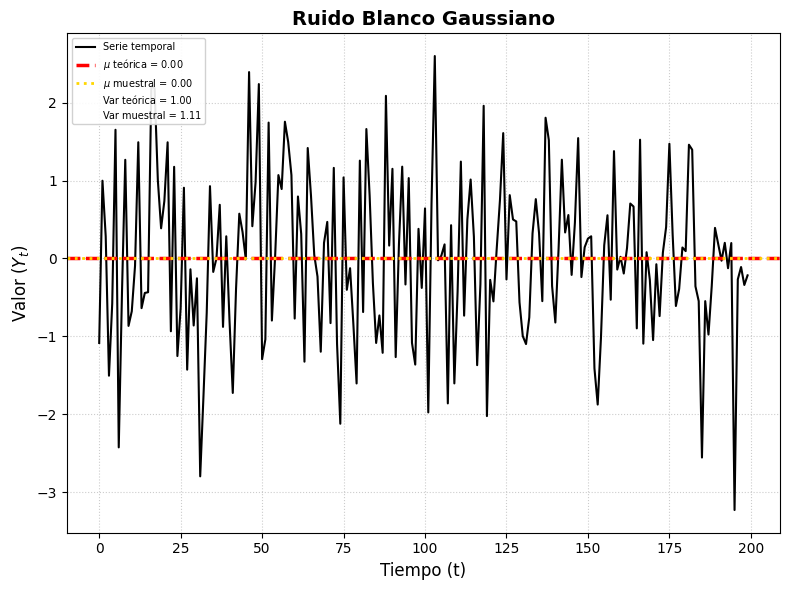
\includegraphics[width=\textwidth]{imagenes/Posibles img/Ruido Blanco.png}
        \caption{Serie Estacionaria ($\mu$ y $\sigma$ constantes)}
        \label{fig:estacionaria}
    \end{subfigure}
    \hfill
    \begin{subfigure}[b]{0.48\textwidth}
        \centering
        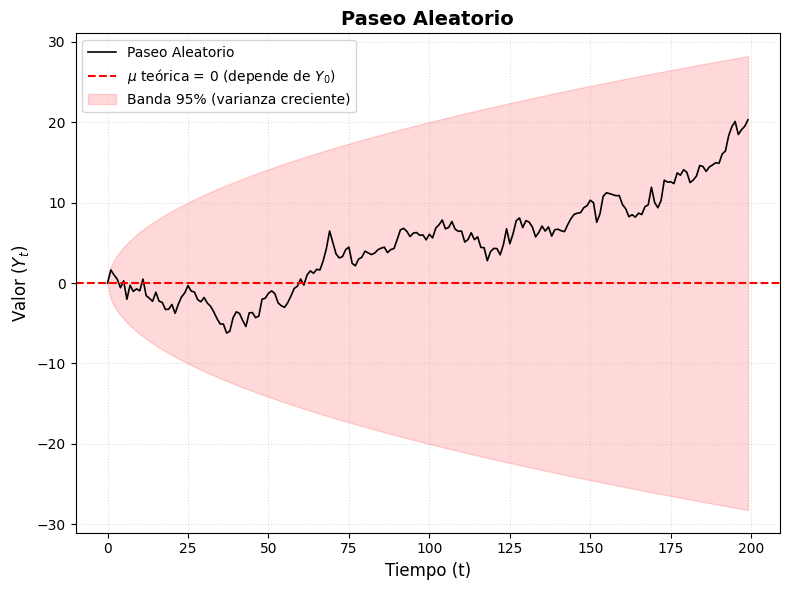
\includegraphics[width=\textwidth]{imagenes/Posibles img/Paseo Aleatorio.png}
        \caption{Serie No Estacionaria($\mu$ y $\sigma$ variables)}
        \label{fig:no_estacionaria}
    \end{subfigure}
    \caption{Ejemplificación de una serie estacionaria y una no estacionarias.}
    \label{fig:comparacion_series}
\end{figure}

\subsection{Estacionalidad múltiple}

Una serie temporal exhibe estacionalidad cuando presenta patrones que se repiten con una periodicidad fija $m$. En el contexto de series temporales de precios eléctricos, es habitual observar estacionalidad en múltiples escalas simultáneamente: un patrón diario de periodo $m_1=24$ horas, asociado al ciclo de demanda residencial e industrial, un patrón semanal de periodo $m_2=168$ horas, determinado por la diferencia entre días hábiles y fines de semana, y un patrón anual de periodo $m_3=8760$ horas, vinculado a la variación estacional de la radiación solar y la hidrología.

La manera natural de modelar esta estructura es mediante una descomposición aditiva:

\begin{equation}
    y_t = T_t + \sum_{j=1}^{J} S_t^{(j)} + \varepsilon_t\quad,
\end{equation}

donde $T_t$ es la componente de tendencia, $S_t^{(j)}$ es la $j$-ésima componente estacional de periodo $m_j$ y $\varepsilon_t \sim \mathcal{N}(0, \sigma^2)$ es el término de error. La idea de este modelo radica en el supuesto de que las fuentes de variación son conceptualmente separables y aditivas: la tendencia captura la dinámica de largo plazo del mercado, cada componente estacional captura un ciclo recurrente de distinta escala, y el residuo recoge la variabilidad no estructurada.

En el contexto de series temporales, una componente estacional $S_t^{(j)}$ de periodo $m$ es por definición una función periódica, por lo que puede representarse mediante una serie de Fourier truncada de orden $K_j$:

\begin{equation}
    S_t^{(j)} = \sum_{k=1}^{K_j} \left[ a_k^{(j)} \cos\left(\frac{2\pi k t}{m_j}\right) + b_k^{(j)} \sin\left(\frac{2\pi k t}{m_j}\right) \right]
    \label{eq:fourier_seasonality}
\end{equation}

donde los coeficientes $\{a_k^{(j)}, b_k^{(j)}\}$ son parámetros estimables. Esta representación viene de la teoría clásica de señales, donde cualquier función periódica de periodo $m$ que sea integrable puede aproximarse mediante sumas de senos y cosenos de frecuencias múltiplos de $\frac{1}{m}$.

Esta representación tiene tres ventajas que la hacen adecuada para su estimación mediante optimización:es diferenciable, lo que permite la optimización por descenso de gradiente, es flexible, pues puede aproximar estacionalidades de cualquier forma y no solo senoidales, y parsimoniosa, lo que permite capturar patrones complejos con pocos coeficientes. El orden $K_j$ controla la suavidad de la estacionalidad estimada: valores pequeños de $K_j$ producen componentes suaves, mientras que valores grandes permiten capturar formas más irregulares.

\begin{figure}[htbp]
    \centering
    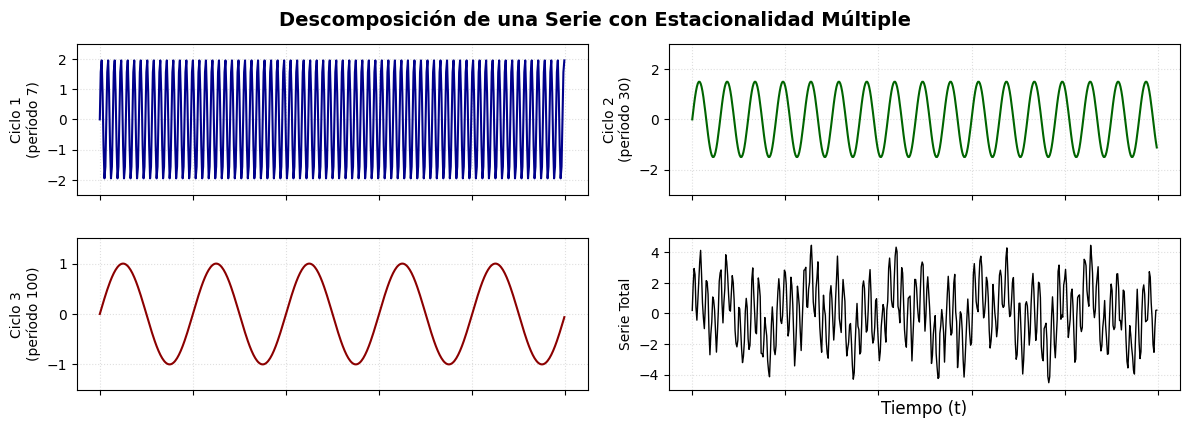
\includegraphics[width=0.9\linewidth]{imagenes/Posibles img/Estacionalidad.png}
    \caption{Visualización de una serie con estacionalidad múltiple descompuesta}
    \label{fig:placeholder}
\end{figure}

\subsection{Procesos no estacionarios y transformaciones}

Cuando una serie presenta tendencia, varianza no constante o cambios estructurales, es necesario aplicar transformaciones previas al entrenamiento para estabilizar sus propiedades estadísticas y mejorar la convergencia de los modelos. La transformación más utilizada en el contexto de modelos de aprendizaje profundo es la \textit{estandarización} o \textit{normalización z-score}, que transforma cada observación según:

\begin{equation}
    \tilde{y}_t = \frac{y_t - \hat{\mu}}{\hat{\sigma}}
\end{equation}

donde $\hat{\mu}$ y $\hat{\sigma}$ son la media y desviación estándar estimadas exclusivamente sobre el conjunto de entrenamiento. Esta transformación garantiza que la serie transformada tenga media cero y varianza unitaria, lo que estabiliza el gradiente durante el entrenamiento y hace que los parámetros del modelo sean comparables entre distintas barras y horizontes. Es fundamental que los parámetros $\hat{\mu}$ y $\hat{\sigma}$ se estimen solo sobre el conjunto de entrenamiento y se apliquen sin reestimación al conjunto de validación y prueba, evitando así la filtración de información futura o \textit{data leakage}. 

Otras transformaciones comunes en la literatura incluyen la diferenciación de orden $d$, que elimina tendencias polinomiales, y la transformación logarítmica, que estabiliza la varianza en series con heterocedasticidad multiplicativa. En este trabajo se adopta la estandarización z-score como transformación principal, aplicada de manera independiente a cada barra del SEN mediante \texttt{StandardScaler}.

\subsection{Horizonte de predicción y estrategia de forecasting multihorizonte}

El horizonte de predicción $h$ determina cuántos pasos adelante se desea predecir. En mercados eléctricos, el horizonte más relevante operacionalmente es el \textit{day-ahead}, es decir, $h=24$ horas, que corresponde al ciclo de programación del despacho en el SEN. En este trabajo se adopta un horizonte de $h=1$ hora, lo que corresponde a la predicción del costo marginal de la hora inmediata siguiente dado una ventana de predicción de longitud $L$. Formalmente, el problema de predicción se define como estimar:

\begin{equation}
    \hat{y}_{t+1} = f\left(y_{t-L+1:t},\, \mathbf{x}_{t-L+1:t+1}\right)
\end{equation}

donde $L$ es la longitud de la ventana de contexto y $\mathbf{x}_t$ denota el vector de covariables exógenas conocidas en el tiempo $t$, como temperatura, demanda o generación, y $f$ es el modelo de forecasting.

Aunque en este trabajo se considera $h=1$, vale la pena situar este caso dentro del marco general de estrategias de forecasting multihorizonte, dado que el TFT fue diseñado para el caso general $h \geq 1$. Las tres estrategias principales son: la estrategia \textit{recursiva}, que aplica iterativamente el modelo de un paso para generar predicciones de múltiples horizontes usando predicciones previas como entrada; la estrategia \textit{directa}, que entrena un modelo independiente para cada horizonte $h$, y la estrategia MIMO (\textit{Multiple Input Multiple Output}), que predice simultáneamente todos los horizontes con un único modelo, capturando las dependencias entre ellos. El TFT adopta la estrategia MIMO, lo que lo hace naturalmente extensible a horizontes mayores si el alcance del trabajo lo permite.

Un concepto distinto pero relacionado con el horizonte de predicción es la \textit{granularidad} o resolución temporal de la serie, es decir, el intervalo de muestreo entre observaciones consecutivas. Mientras el horizonte $h$ determina cuántos pasos futuros se predicen, la granularidad determina la duración real de cada paso: una serie horaria y una serie de 15 minutos pueden compartir el mismo horizonte $h=1$ en número de pasos, pero constituyen problemas de predicción distintos, con distinta cantidad de observaciones por unidad de tiempo y, potencialmente, distinta relación señal-ruido en la ventana de contexto $L$. El pipeline principal de este trabajo se construye sobre datos horarios, resolución que coincide con el ciclo de programación y liquidación del costo marginal en el SEN; el Capítulo 4 explora de manera preliminar el efecto de contrastar esta resolución con series diarias y de 15 minutos sobre el desempeño del modelo.

\subsection{Forecasting multivariado y estructura de barras}

En este trabajo el problema de forecasting no se limita a una única serie, sino que se extiende a $B = 8$ barras del SEN, cada una con su propia serie de costos marginales horarios$\{y_t^{(b)}\}_{t=1}^{T} \, \text{con} \quad b=1, ...,8$. Este escenario define un problema de forecasting multivariado, donde las series pueden presentar dependencias cruzadas, por ejemplo, barras eléctricamente contiguas tienden a exhibir costos marginales correlacionados, salvo en episodios de congestión de transmisión, donde los precios se desacoplan, generando heterogeneidad estructural entre barras. 

Esta correlación entre barras puede cuantificarse formalmente mediante una función de correlación cruzada, lo que en principio permitiría un enfoque de \textit{forecasting con dependencias espaciales}, donde la predicción para la barra $b$ incorpora información de las barras vecinas. Sin embargo, este enfoque requiere modelar explícitamente la topología de la red eléctrica y puede introducir complejidad adicional cuando las congestiones generan desacoplamientos no estacionarios entre barras.

La estrategia adoptada en este trabajo consiste en entrenar un modelo independiente por barra, lo cual simplifica el problema a costa de ignorar las dependencias cruzadas. Esta decisión se justifica por dos razones: las congestiones de transmisión en el SEN introducen heterogeneidad estructural entre barras que dificultaría el entrenamiento conjunto, y los modelos independientes son más interpretables y permiten identificar con claridad el comportamiento especifico de cada barra. La incorporación de dependencias espaciales mediante correlación cruzada queda propuesta como una extensión natural de este trabajo para investigación futura.

\section{Prophet}

Prophet es un modelo de \textit{forecasting} de series temporales desarrollado por Taylor y Letham (2018) en Meta \cite{Prophet}, diseñado para producir predicciones interpretables en series con patrones estacionales fuertes, valores faltantes (\textit{missing values}) y cambios de tendencia abruptos. A diferencia de los modelos estadísticos clásicos como ARIMA y sus variantes, Prophet no requiere que la serie sea estacionaria ni impone supuestos sobre la estructura de autocorrelación de los residuos. Su diseño está orientado a la estimación automática de componentes interpretables, lo que lo hace especialmente adecuado como componente de descomposición en arquitecturas híbridas.

Prophet formula el problema de forecasting como la estimación de un modelo aditivo de la forma:

\begin{equation}
\hat{y}_t^{Prophet} = T(t) + S(t) + H(t) + \varepsilon_t
\end{equation}

donde $T(t)$ es la componente de tendencia, $S(t)$ es la componente de estacionalidad, $H(t)$ captura el efecto de días festivos y eventos especiales, y $\varepsilon_t \sim \mathcal{N}(0, \sigma^2)$ es el término de error. Cada componente se estima de manera independiente, lo que otorga al modelo su interpretabilidad característica. La estimación de los parámetros se realiza mediante inferencia bayesiana con el software Stan, lo que permite incorporar incertidumbre en las predicciones de manera natural.

\subsection{Componente de tendencia}

Prophet ofrece dos especificaciones para la componente de tendencia $T(t)$. La primera es un \textit{modelo de crecimiento logístico}, adecuado para trabajar con series que tienen un capacidad máxima o saturación:

\begin{equation}
T(t) = \frac{C}{1 + e^{-k(t - m)}}
\end{equation}

donde $C$ es la capacidad de saturación, $k$ es la tasa de crecimiento y $m$ es el punto de inflexión. La segunda, y más utilizada en series de precios, es un \textit{modelo lineal por tramos} (\textit{piecewise linear}):

\begin{equation}
T(t) = (k + \mathbf{a}(t)^\top \boldsymbol{\delta})t + (m + \mathbf{a}(t)^\top \boldsymbol{\gamma})
\end{equation}

donde $k$ es la tasa de crecimiento global, $\boldsymbol{\delta} \in \mathbb{R}^S$ es el vector de cambios de pendiente en cada uno de los $S$ puntos de quiebre, $\mathbf{a}(t) \in \{0,1\}^S$ es un vector indicador que activa los cambios acumulados hasta el tiempo $t$, y $\boldsymbol{\gamma}$ ajusta el intercepto para garantizar continuidad en los puntos de quiebre. Los puntos de quiebre pueden especificarse manualmente o detectarse automáticamente por el modelo, lo que le permite adaptarse a cambios estructurales graduales como los que experimenta el costo marginal del SEN ante la incorporación continua de capacidad renovable.

La detección automática de los puntos de quiebre se realiza colocando una distribución a priori dispersa sobre los ajustes de pendiente $\boldsymbol{\delta} \sim \text{Laplace}(0, \tau)$, donde $\tau > 0$ controla la flexibilidad del modelo. Un prior disperso permite que Prophet proponga un gran número de puntos de quiebre candidatos, típicamente uno por mes en una historia de varios años, pero penaliza aquellos ajustes que no son necesarios para explicar los datos. Cuando $\tau \to 0$, el modelo reduce a una tendencia lineal o logística simple sin quiebres. Este mecanismo de regularización es especialmente relevante para las series de costos marginales del SEN, donde los cambios estructurales son graduales y difíciles de datar con precisión \cite{Prophet}.

\subsection{Componente de estacionalidad}

La componente estacional $S(t)$ se modela como la suma de las componentes de Fourier truncadas $S_t^{(j)}$ de la Ecuación \eqref{eq:fourier_seasonality} (Sección 2.1.2) sobre las $J$ escalas estacionales consideradas, $S(t) = \sum_{j=1}^{J} S_t^{(j)}$. El orden $K_j$ controla la flexibilidad de cada componente estacional: Prophet usa por defecto $K=10$ para la estacionalidad anual y $K=3$ para la semanal, valores que pueden ajustarse según la complejidad de los patrones observados. En este trabajo se consideran las estacionalidades diaria ($m_1 = 24$), semanal ($m_2 = 168$) y anual ($m_3 = 8760$), capturando los tres ciclos recurrentes identificados en la Sección 2.1.

\subsection{Componente de festividades y eventos especiales}

La componente $H(t)$ modela el efecto de días festivos y eventos especiales que producen desviaciones sistemáticas en la serie, no capturables por la estacionalidad regular. Prophet representa este efecto como:

\begin{equation}
H(t) = \mathbf{Z}(t)\boldsymbol{\kappa}
\end{equation}

donde $\mathbf{Z}(t) \in \{0,1\}^{L}$ es un vector indicador que activa el evento correspondiente al tiempo $t$, y $\boldsymbol{\kappa} \in \mathbb{R}^{L}$ es el vector de efectos estimados para cada uno de los $L$ eventos definidos. En este trabajo se incorporan los feriados nacionales del calendario chileno, dado que el consumo eléctrico y el despacho del SEN exhiben patrones sistemáticamente distintos en días festivos respecto a días hábiles.

\subsection{Estimación e inferencia}

Análogamente al prior sobre el cambio de tendencia $\boldsymbol{\delta}$ (Sección 2.2.1), los coeficientes estacionales reciben una distribución a priori $\boldsymbol{\beta} \sim \mathcal{N}(0, \sigma_s^2)$, donde $\sigma_s$ es el hiperparámetro \texttt{seasonality\_prior\_scale} que regula la flexibilidad de la estacionalidad, ajustado por barra junto con $\tau$ en la Sección 3.3.1. La inferencia se realiza mediante \textit{Maximum A Posteriori} (MAP), suficiente para los fines de este trabajo dado que la cuantificación de incertidumbre de las predicciones finales se aborda mediante el TFT y Conformal Prediction (Secciones 2.3.4 y 2.6), y no mediante los intervalos de credibilidad bayesianos de Prophet.

\subsection{Rol de Prophet en la arquitectura híbrida}

En el modelo propuesto en este trabajo, Prophet cumple el rol de componente de descomposición temporal. Dado que Prophet modela explícitamente la tendencia, la estacionalidad múltiple y los efectos de calendario, sus predicciones capturan la estructura sistemática de largo plazo de la serie. Los residuos de Prophet:

\begin{equation}
r_t = y_t - \hat{y}_t^{\text{Prophet}}
\end{equation}

representan la variabilidad no explicada por la estructura sistemática, episodios de sobreoferta renovable, congestiones de transmisión y fluctuaciones de corto plazo, que son precisamente las componentes que el TFT está mejor equipado para modelar. Esta separación de roles motiva el diseño de dos modelos TFT paralelos: uno entrenado sobre los residuos $\{r_t\}$ y otro entrenado directamente sobre la serie original $\{y_t\}$, las predicciones se combinan con las hechas por Prophet posteriormente mediante Stacking Optimization, como se detalla en la Sección 2.5.

Esta descripción corresponde específicamente a la rama \textbf{Prophet+Clima (P+C)} del modelo propuesto en este trabajo. La Sección 2.3.5 presenta el rol del TFT dentro de esta rama junto con el de la rama alternativa \textbf{Sol+Clima (S+C)}, que prescinde por completo de Prophet.

\section{Transformer y Temporal Fusion Transformer}

El mecanismo de atención y la arquitectura Transformer, introducidas por Vaswani et al. (2017) \cite{Vaswani2017Attention} revolucionaron el procesamiento secuencial de datos y el \textit{Deep Learning}. Hasta entonces, los dos paradigmas dominantes para el modelado de secuencias eran las arquitecturas recurrentes, en particular las \textit{Redes Neuronales Recurrentes} (RNN) y los modelos de \textit{Memoria Larga a Corto Plazo} (LSTM), y las arquitecturas convolucionales aplicadas a secuencias. Ambas familias presentaban limitaciones complementarias: las recurrentes procesaban la secuencia de forma inherentemente secuencial, lo que impedía su paralelización durante el entrenamiento, mientras que las convolucionales, aunque paralelizables, requerían apilar múltiples capas para capturar dependencias de largo alcance. El Transformer elimina simultáneamente la recurrencia y la convolución, reemplazándolas por un mecanismo de auto-atención que conecta cualquier par de posiciones de la secuencia en un número constante de operaciones, permitiendo tanto la paralelización completa del entrenamiento como el modelado directo de dependencias de largo alcance \cite{Vaswani2017Attention}. En esta sección se presenta primero el mecanismo de atención y la arquitectura Transformer clásica, para luego describir el \textit{Temporal Fusion Transformer} (TFT), la variante especializada para forecasting multihorizonte utilizada en este trabajo.

\subsection{Mecanismo de atención}

El mecanismo de atención permite que un modelo pondere diferencialmente la relevancia de distintas posiciones de una secuencia al producir una representación para cada posición. La idea central es que, al predecir el valor en el tiempo $t$, no todas las observaciones pasadas son igual de relevantes, algunas tienen mayor influencia que otras dependiendo del contexto.

Formalmente, el mecanismo de atención opera sobre tres matrices: las \textit{queries} $\mathbf{Q} \in \mathbb{R}^{n \times d_k}$, las \textit{keys} $\mathbf{K} \in \mathbb{R}^{m \times d_k}$ y los \textit{values} $\mathbf{V} \in \mathbb{R}^{m \times d_v}$, donde $n$ es el número de posiciones de consulta, $m$ el número de posiciones de referencia, $d_k$ la dimensión de las queries y keys, y $d_v$ la dimensión de los values. La salida del mecanismo de atención es:

\begin{equation}
\text{Attention}(\mathbf{Q}, \mathbf{K}, \mathbf{V}) = \text{softmax}\left(\frac{\mathbf{Q}\mathbf{K}^\top}{\sqrt{d_k}}\right)\mathbf{V}
\end{equation}

El término $\mathbf{Q}\mathbf{K}^\top \in \mathbb{R}^{n \times m}$ calcula los productos punto entre cada query y cada key, produciendo una matriz de \textit{scores} que mide la afinidad entre pares de posiciones. La división por $\sqrt{d_k}$ estabiliza los gradientes durante el entrenamiento: sin este factor, cuando $d_k$ es grande los productos punto crecen en magnitud y empujan a la función softmax hacia regiones de gradiente muy pequeño. La función softmax normaliza los \textit{scores} por filas, produciendo para cada posición una combinación convexa ponderada de los values de las posiciones de referencia. Este mecanismo se denomina \textit{scaled dot-product attention} y tiene complejidad computacional $\mathcal{O}(n \cdot m \cdot d_k)$ en tiempo y $\mathcal{O}(n \cdot m)$ en memoria, lo que puede ser restrictivo para secuencias largas.

\subsection{Atención multi-cabeza}

En la práctica, es beneficioso que el modelo pueda atender a distintos tipos de relaciones simultáneamente, por ejemplo, dependencias de corto plazo y de largo plazo al mismo tiempo. La \textit{atención multi-cabeza} (\textit{multi-head attention}) logra esto proyectando las queries, keys y values en $H$ subespacios distintos y calculando la atención en cada uno, de forma paralela:

\begin{equation}
\text{MultiHead}(\mathbf{Q}, \mathbf{K}, \mathbf{V}) = \text{Concat}(\text{head}_1, \ldots, \text{head}_H) \,\mathbf{W}^O
\end{equation}

donde cada cabeza se define como:

\begin{equation}
\text{head}_h = \text{Attention}(\mathbf{Q}\mathbf{W}_h^Q, \mathbf{K}\mathbf{W}_h^K, \mathbf{V}\mathbf{W}_h^V)
\end{equation}

con matrices de proyección $\mathbf{W}_h^Q \in \mathbb{R}^{d_{\text{model}} \times d_k}$, $ \mathbf{W}_h^K \in \mathbb{R}^{d_{\text{model}} \times d_k}$, $\mathbf{W}_h^V \in \mathbb{R}^{d_{\text{model}} \times d_v}$ y $\mathbf{W}^O \in \mathbb{R}^{H d_v \times d_{\text{model}}}$. Típicamente se fija $d_k = d_v = d_{\text{model}} / H$ para mantener el costo computacional equivalente al de una sola cabeza de dimensión completa.

\subsection{Arquitectura Transformer}

El Transformer completo apila $N$ bloques idénticos, alternando una capa de atención multi-cabeza y una red de alimentación directa (\textit{Feed-Forward Network}, FFN), ambas envueltas en conexiones residuales y normalización de capa, e incorpora una \textit{codificación posicional} (\textit{positional encoding}) senosoidal para inyectar el orden temporal de la secuencia, dado que el mecanismo de atención es en sí mismo invariante a permutaciones \cite{Vaswani2017Attention}. El Temporal Fusion Transformer, descrito en la Sección 2.3.4, se aparta de esta arquitectura genérica en dos aspectos centrales: reemplaza el bloque residual y la codificación posicional por una etapa de procesamiento secuencial local basada en LSTM (Sección 2.3.4.4), y sustituye la atención multi-cabeza estándar por un mecanismo de atención interpretable que comparte los values entre cabezas (Sección 2.3.4.6), conservando no obstante la formulación de \textit{queries}, \textit{keys} y \textit{values} presentada en esta sección.

\subsection{Temporal Fusion Transformer}

El Temporal Fusion Transformer (TFT), propuesto por Lim et al. (2021) \cite{TFT}, extiende la arquitectura Transformer para el problema específico de forecasting multihorizonte con covariables heterogéneas. A diferencia del Transformer clásico, el TFT incorpora mecanismos explícitos para el manejo de covariables estáticas, selección de variables relevantes, procesamiento secuencial local e interpretabilidad de las dependencias temporales aprendidas. La arquitectura se organiza en cinco componentes principales que se describen a continuación.

\subsubsection{Codificación de entradas y embeddings}

El TFT recibe tres tipos de entradas: covariables estáticas $\mathbf{s} \in \mathbb{R}^{d_s}$, que no varían en el tiempo, por ejemplo, el identificador de barra, covariables temporales pasadas conocidas $\mathbf{x}_{t-L:t} \in \mathbb{R}^{L \times d_x}$ y covariables temporales futuras conocidas $\mathbf{x}_{t:t+H} \in \mathbb{R}^{H \times d_x}$, por ejemplo, el día de la semana o el indicador de feriado. Cada variable es proyectada a un espacio de representación de dimensión $d_{\text{model}}$ mediante transformaciones lineales o embeddings aprendibles.

\subsubsection{Gated Residual Network}

El bloque fundamental del TFT es la \textit{Gated Residual Network} (GRN), que permite al modelo suprimir información irrelevante mediante una compuerta aprendible:

\begin{equation}
\text{GRN}(\mathbf{a}, \mathbf{c}) = \text{LayerNorm}\left(\mathbf{a} + \text{GLU}\left(\mathbf{W}_1 \, \text{ELU}(\mathbf{W}_2 \, \mathbf{a} + \mathbf{W}_3 \, \mathbf{c} + \mathbf{b}_2) + \mathbf{b}_1\right)\right)
\end{equation}

donde $\mathbf{a}$ es la entrada principal, $\mathbf{c}$ es un contexto opcional, ELU es la función de activación exponencial lineal, y GLU (\textit{Gated Linear Unit}) es el mecanismo de compuerta definido como:

\begin{equation}
\text{GLU}(\mathbf{h}) = \sigma(\mathbf{W}_4 \, \mathbf{h} + \mathbf{b}_3) \odot (\mathbf{W}_5 \, \mathbf{h} + \mathbf{b}_4)
\end{equation}

donde $\sigma$ es la función sigmoide y $\odot$ denota el producto de Hadamard. La compuerta $\sigma(\cdot)$ puede aprender a anular completamente la contribución del bloque cuando la entrada no es informativa, lo que dota al TFT de una capacidad de regularización adaptativa que el Transformer clásico no posee.

\subsubsection{Variable Selection Network}

La \textit{Variable Selection Network} (VSN) extiende la idea de la GRN para seleccionar, de manera suave y diferenciable, cuáles de las $m_\chi$ covariables disponibles son más relevantes para la predicción en cada paso temporal. Dada la concatenación $\Xi_t$ de las representaciones de todas las covariables en el tiempo $t$, la VSN genera pesos de selección mediante una GRN seguida de una función softmax:

\begin{equation}
\mathbf{v}_t^\chi = \text{Softmax}\left(\text{GRN}_{v_\chi}\left(\Xi_t, \, \mathbf{c}_s\right)\right)
\end{equation}
 
donde $\mathbf{c}_s$ es el vector de contexto derivado de las covariables estáticas mediante un encoder separado. Cada covariable $j$ es además procesada por su propia GRN antes de la ponderación:

\begin{equation}
\tilde{\xi}_t = \sum_{j=1}^{m_\chi} v^{(j)}_{\chi_t} \cdot \tilde{\xi}^{(j)}_t
\end{equation}

donde $v^{(j)}_{\chi_t}$ es el $j$-ésimo elemento del vector $\mathbf{v}^\chi_t$ y $\tilde{\xi}^{(j)}_t$ es la representación procesada de la covariable $j$ en el tiempo $t$. Los pesos $v^{(j)}_{\chi_t}$ son interpretables y permiten identificar qué variables exógenas contribuyen más a la predicción en cada instante.

\subsubsection{Procesamiento secuencial local}

Antes de aplicar la atención global, el TFT procesa la secuencia temporal mediante una capa sequence-to-sequence basada en LSTM para capturar dependencias locales de corto plazo. El diseño usa un LSTM encoder para las entradas pasadas y un LSTM decoder para las entradas futuras conocidas, ambos unidireccionales para preservar la causalidad:

\begin{align}
    \left[\mathbf{h}_{t-L}, \ldots, \mathbf{h}_t\right] &= \text{LSTM}_{\text{enc}}\left(\left[\tilde{\xi}_{t-L}, \ldots, \tilde{\xi}_t\right]\right) \\
    \left[\mathbf{h}_{t+1}, \ldots, \mathbf{h}_{t+H}\right] &= \text{LSTM}_{\text{dec}}\left(\left[\tilde{\xi}_{t+1}, \ldots, \tilde{\xi}_{t+H}\right]\right)
\end{align}

donde los estados iniciales del LSTM decoder se inicializan con vectores de contexto $\mathbf{c}_c$ y $\mathbf{c}_h$ derivados de las covariables estáticas, lo que permite que la información estática condicione el procesamiento local. Las salidas del LSTM se conectan al resto de la arquitectura mediante una conexión residual con compuerta (\textit{Gated Skip Connection}):

\begin{equation}
\tilde{\phi}(t, n) = \text{LayerNorm}\!\left(\tilde{\xi}_{t+n} + \text{GLU}_{\tilde{\phi}}\!\left(\phi(t, n)\right)\right)
\end{equation}

donde $\phi(t, n)$ es la salida del LSTM en la posición $n$ relativa al tiempo de forecast $t$. Esta conexión residual cumple un rol de regularización: si el procesamiento local no aporta información, la compuerta GLU puede suprimirlo completamente, permitiendo que el flujo de información saltee la capa y degradando el modelo graciosamente hacia una arquitectura más simple \cite{TFT}.
 
Dado que en este trabajo $H = 1$, la distinción encoder/decoder colapsa a una única pasada hacia adelante sobre la ventana de contexto, simplificando la notación a:

\begin{equation}
\left[\mathbf{h}_{t-L}, \ldots, \mathbf{h}_t\right] = \text{LSTM}\left(\left[\tilde{\xi}_{t-L}, \ldots, \tilde{\xi}_t\right]\right)
\end{equation}

Esta combinación de LSTM y Transformer permite al TFT capturar tanto dependencias locales, a través del LSTM, como dependencias de largo alcance, a través de la atención.

\subsubsection{Enriquecimiento estático}

Las covariables estáticas, como el identificador de barra en este trabajo, no solo actúan como contexto para la selección de variables: el TFT les dedica una capa explícita de \textit{enriquecimiento estático} que inyecta información estática directamente en las representaciones temporales antes de que estas entren al bloque de auto-atención. Formalmente, para cada posición $n$ de la secuencia, la capa aplica una GRN condicionada por el vector de contexto estático $\mathbf{c}_e$:
 
\begin{equation}
\theta(t, n) = \text{GRN}_\theta\!\left(\tilde{\phi}(t, n),\; \mathbf{c}_e\right)
\end{equation}
 
donde $\tilde{\phi}(t, n)$ es la representación local producida por la capa LSTM con su conexión residual y los pesos de la GRN son compartidos a lo largo de toda la secuencia. El efecto es que cada representación temporal queda condicionada por la identidad de la entidad, en este caso la barra eléctrica, permitiendo al modelo aprender dinámicas temporales distintas para cada nodo del sistema sin necesidad de entrenar instancias separadas \cite{TFT}.

\subsubsection{Atención temporal interpretable}

El TFT reemplaza la atención multi-cabeza estándar por una variante interpretable en la que todas las cabezas comparten la misma matriz de values:

\begin{equation}
\text{InterpretableAttention}(\mathbf{Q}, \mathbf{K}, \mathbf{V}) = \tilde{\mathbf{A}}\mathbf{V}\mathbf{W}_V
\end{equation}

\begin{equation}
\tilde{\mathbf{A}} = \frac{1}{H}\sum_{h=1}^{H} \text{softmax}\left(\frac{\mathbf{Q}\mathbf{W}_h^Q (\mathbf{K}\mathbf{W}_h^K)^\top}{\sqrt{d_k}}\right)
\end{equation}

Al compartir los values entre cabezas y promediar las matrices de atención, el TFT produce una única matriz $\tilde{\mathbf{A}}$ que puede visualizarse directamente para identificar qué instantes temporales del pasado son más relevantes para la predicción. Esta propiedad es especialmente valiosa en el contexto del SEN, donde identificar qué horas o días del pasado influyen más en el costo marginal tiene valor interpretativo directo para los operadores del sistema.

Un requisito fundamental en forecasting es que el modelo no pueda acceder a observaciones futuras al generar una predicción, es decir, que la atención respete la causalidad temporal. El TFT garantiza esto mediante \textit{enmascaramiento causal} (\textit{decoder masking}): en la matriz de scores $\mathbf{Q}\mathbf{W}_h^Q(\mathbf{K}\mathbf{W}_h^K)^\top$, todas las entradas que corresponden a posiciones futuras respecto al horizonte de predicción se fijan en $-\infty$ antes de aplicar la función softmax, lo que hace que sus pesos de atención sean exactamente cero tras la normalización \cite{Vaswani2017Attention, TFT}. Formalmente, el elemento $(i,j)$ de la matriz de atención satisface $\tilde{\mathbf{A}}_{ij} = 0$ para todo $j > i$. En el contexto de este trabajo, donde se predicen costos marginales horarios con datos del mercado eléctrico chileno, esta restricción no es solo una convención arquitectónica sino una condición de validez del modelo: permitir que la atención alcance instantes futuros equivaldría a filtración de información (\textit{data leakage}) y produciría métricas de evaluación artificialmente optimistas.

\subsubsection{Salidas cuantílicas}

A diferencia del Transformer clásico que produce predicciones puntuales, el TFT genera predicciones para múltiples cuantiles $q \in \mathcal{Q}$ simultáneamente mediante capas lineales independientes aplicadas a la representación final:

\begin{equation}
\hat{y}_t^{(q)} = \mathbf{W}_q \, \mathbf{h}_t + \mathbf{b}_q \quad \forall\, q \in \mathcal{Q}
\end{equation}

El modelo se entrena minimizando la pérdida de regresión cuantílica sumada sobre todos los cuantiles y horizontes:

\begin{equation}
\mathcal{L} = \sum_{q \in \mathcal{Q}} \sum_{t} \mathcal{L}_q\left(y_t, \, \hat{y}_t^{(q)}\right)
\label{eq:quantile_loss_sum}
\end{equation}

donde la pérdida cuantílica para el cuantil $q$ es:

\begin{equation}
\mathcal{L}_q(y, \hat{y}) = \max\left(q(y - \hat{y}), \, (q-1)(y - \hat{y})\right)
\end{equation}

Esta formulación garantiza que $\hat{y}_t^{(q)}$ converja al cuantil $q$ de la distribución condicional de $Y_t$, proporcionando intervalos de predicción sin supuestos distribucionales cuando el modelo se entrena con esta pérdida. En este trabajo, sin embargo, el TFT se entrena minimizando directamente el MAE de la predicción puntual, el caso particular de \eqref{eq:quantile_loss_sum} con un único cuantil $q=0.5$, lo que permite aplicar \textit{early stopping} directamente sobre la métrica objetivo del problema en lugar de sobre una suma de pérdidas cuantílicas. La cuantificación de incertidumbre no se delega, por lo tanto, a salidas cuantílicas del TFT, sino que se aborda íntegramente mediante Conformal Prediction (Sección 2.6), aplicado sobre la predicción puntual resultante.

\subsection{Rol del TFT en la arquitectura híbrida}

El TFT es el componente común a las dos estrategias de construcción de \textit{features} comparadas en este trabajo, P+C y S+C, pero su rol dentro de cada una difiere sustancialmente.

En la estrategia \textbf{P+C}, descrita en la Sección 2.2.6, se entrenan dos instancias del TFT en paralelo: una sobre los residuos de Prophet $\{r_t\}$ y otra directamente sobre la serie original $\{y_t\}$. La primera instancia captura la variabilidad de corto plazo no explicada por la descomposición sistemática de Prophet, mientras que la segunda modela la serie completa sin restricciones de descomposición. Ambas instancias se comparan mediante las mismas métricas de evaluación, y sus predicciones, junto con las de Prophet, se combinan posteriormente mediante Stacking Optimization, como se detalla en la Sección 2.5. Adicionalmente, las componentes descompuestas por Prophet, la tendencia $T(t)$, la estacionalidad $S(t)$ y el efecto de festividades $H(t)$, se incorporan como covariables exógenas conocidas en ambas instancias del TFT, permitiendo que el modelo de atención explote explícitamente la estructura temporal identificada por Prophet al construir sus representaciones.

En la estrategia \textbf{S+C}, en cambio, se entrena una única instancia del TFT directamente sobre la serie de precios $\{y_t\}$, sin residuos de Prophet ni ensamblaje posterior mediante Stacking. Las covariables conocidas dejan de ser las componentes de Prophet y pasan a ser variables de posición solar (elevación solar y horario de verano), calculadas de forma directa a partir de la geolocalización de cada barra en lugar de estimarse mediante un modelo de descomposición intermedio. La motivación y el detalle completo de ambas estrategias, incluyendo su construcción de \textit{features}, se presentan en la Sección 3.4.1; los resultados de su comparación empírica, en el Capítulo 4.

\section{Layer Normalization y Dynamic Tanh}
 
Las capas de normalización son uno de los componentes fundamentales de las redes neuronales profundas modernas. Su adopción masiva está impulsada por sus beneficios empíricos en la optimización: aceleran la convergencia, estabilizan el entrenamiento y reducen la sensibilidad a la inicialización de parámetros \cite{LNInTransformers}. En la arquitectura Transformer, y por extensión en el TFT, la normalización de capa o \textit{Layer Normalization} (LayerNorm) aparece en cada bloque de la red: dentro de las GRN, alrededor de las capas de atención y en las conexiones residuales. Su presencia es tan sistemática que ha llegado a considerarse indispensable. En este trabajo se reemplaza LayerNorm por \textit{Dynamic Tanh} (DyT) \cite{Zhu2025Transformers} en toda la arquitectura TFT, lo que constituye una de las contribuciones de diseño del modelo propuesto. En esta sección se presenta primero la formulación y propiedades de LayerNorm, luego se analiza el comportamiento empírico que motivó el desarrollo de DyT, y finalmente se describe DyT y se fundamenta su uso en el contexto de este trabajo.
 
\subsection{Layer Normalization}
 
La normalización de capa, propuesta por Ba et al. (2016) \cite{LNBa}, opera de manera independiente para cada token en cada muestra del \textit{batch}. Dado un vector de activaciones $\mathbf{x} \in \mathbb{R}^C$, donde $C$ es la dimensión del embedding, LayerNorm calcula la media $\mu$ y la varianza $\sigma^2$ sobre las $C$ dimensiones del propio vector y normaliza:
 
\begin{equation}
\text{LayerNorm}(\mathbf{x}) = \boldsymbol{\gamma} \cdot \frac{\mathbf{x} - \mu}{\sqrt{\sigma^2 + \epsilon}} + \boldsymbol{\beta}
\end{equation}
 
donde:
$$\mu = \frac{1}{C}\sum_{k=1}^{C} x_k, \qquad \sigma^2 = \frac{1}{C}\sum_{k=1}^{C}(x_k - \mu)^2
$$
 
y $\boldsymbol{\gamma}, \boldsymbol{\beta} \in \mathbb{R}^C$ son parámetros afines aprendibles, denominados, respectivamente, parámetros de escala y de desplazamiento, que permiten que la salida adopte cualquier rango. El término $\epsilon > 0$ es una constante pequeña para estabilidad numérica.
 
A diferencia de la normalización por \textit{batch} (\textit{Batch Normalization}), que calcula estadísticas a través de muestras del \textit{batch} y posiciones temporales, LayerNorm calcula las estadísticas de manera completamente local para cada token en cada muestra, lo que la hace independiente del tamaño del \textit{batch} y adecuada para secuencias de longitud variable. Esta propiedad es especialmente importante en el contexto del TFT, donde el tamaño del \textit{batch} puede variar y las secuencias temporales tienen estructura heterogénea.
 
El rol funcional de LayerNorm en el Transformer es doble. En primer lugar, centra y escala las activaciones para mantenerlas en un rango controlado, lo que estabiliza el flujo de gradientes a través de las capas profundas. En segundo lugar, al operar por token, introduce una no-linealidad implícita: aunque la operación de centrado y escalado es lineal para cada token individualmente, la diversidad de medias y varianzas entre tokens hace que la transformación completa sobre todas las activaciones del tensor sea no-lineal.
 
\subsection{Comportamiento empírico de LayerNorm: curvas tipo tanh}
 
Un resultado empírico central del trabajo de Zhu et al. (2025) \cite{Zhu2025Transformers} es que las capas LayerNorm en Transformers entrenados producen, de manera consistente y no trivial, mapeos entrada-salida con forma de curva en $S$, estadísticamente similares a la función $\tanh$. Este comportamiento fue documentado en tres arquitecturas Transformer de dominios distintos: Vision Transformer (ViT), modelos de habla (wav2vec 2.0) y modelos de difusión (DiT), observándose el mismo patrón en todos los casos para las capas más profundas de la red.

\vspace{0.5cm}
\begin{figure}[htbp]
    \centering
    \begin{subfigure}[b]{0.45\textwidth}
        \centering
        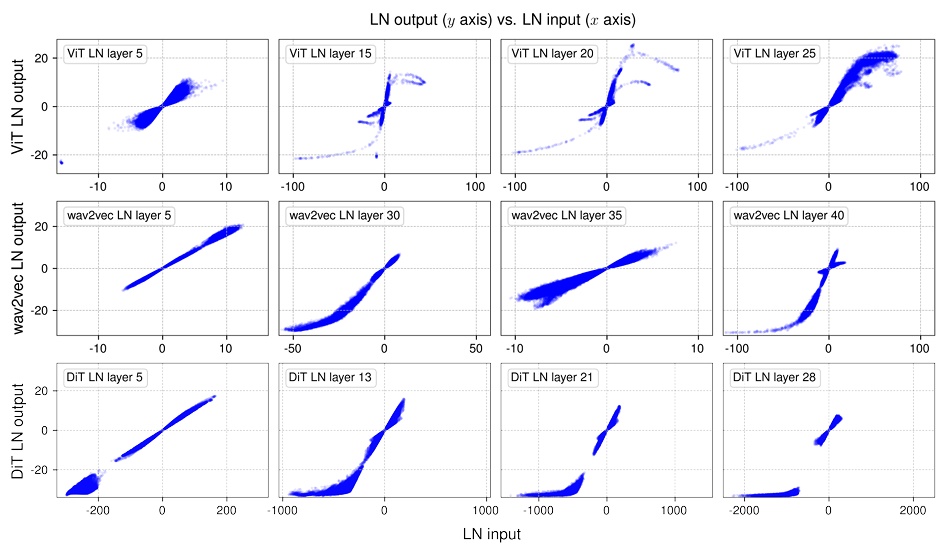
\includegraphics[width=\textwidth]{imagenes/Posibles img/LN en S.png}
        \caption{Entrada-salida producidas por LayerNorm.}
        \label{fig:ln_curva_s}
    \end{subfigure}
    \hfill
    \begin{subfigure}[b]{0.45\textwidth}
        \centering
        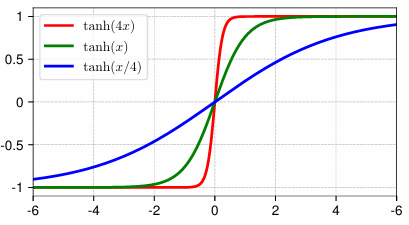
\includegraphics[width=\textwidth]{imagenes/Posibles img/Tanh.png}
        \caption{$\tanh(\alpha x)$ con tres valores diferentes de $\alpha$}
        \label{fig:tanh_alpha}
    \end{subfigure}
    \caption{Similitud entre los mapeos entrada-salida de LayerNorm y la función $\tanh$ escalada.}
    \label{fig:ln_vs_tanh}
\end{figure}
 
Para entender por qué emergen estas curvas, es útil notar que LayerNorm realiza una transformación lineal independiente para cada token. Dado el token $i$, todos sus elementos $x_{ik}$ se escalan por el mismo factor $1/\sigma_i$. Sin embargo, como cada token tiene una varianza distinta, las pendientes de estas transformaciones lineales son distintas entre sí. Cuando se visualizan en conjunto todas las activaciones del tensor, los segmentos de recta de distintas pendientes se ensamblan formando una curva en $S$ no-lineal. Las pocas activaciones con valores extremos, aquellas con $|x_{ik}|$ grande, son las más afectadas por la normalización, pues sus varianzas son altas y el factor $1/\sigma_i$ las comprime fuertemente. Este efecto de \textit{squashing} no-lineal sobre valores extremos es, según Zhu et al. (2025), la propiedad esencial de LayerNorm que explica su importancia en el entrenamiento de redes profundas.
 
Esta observación tiene una implicación directa: si el comportamiento funcional de LayerNorm es empíricamente similar al de una función $\tanh$ escalada, entonces una operación definida explícitamente como $\tanh(\alpha \mathbf{x})$ podría reproducir dicho comportamiento de manera más directa, sin necesidad de calcular estadísticas de activación.
 
\subsection{Dynamic Tanh (DyT)}
 
Inspirados por la similitud entre los mapeos de LayerNorm y la función $\tanh$, Zhu et al. (2025) \cite{Zhu2025Transformers} proponen \textit{Dynamic Tanh} (DyT) como un reemplazo directo (\textit{drop-in replacement}) de las capas de normalización en Transformers. Para un tensor de entrada $\mathbf{x}$, una capa DyT se define como:
 
\begin{equation}
\text{DyT}(\mathbf{x}) = \boldsymbol{\gamma} \cdot \tanh(\alpha \mathbf{x}) + \boldsymbol{\beta}
\end{equation}
 
donde $\alpha \in \mathbb{R}$ es un escalar aprendible que controla la escala de la entrada antes de la función $\tanh$, y $\boldsymbol{\gamma}, \boldsymbol{\beta} \in \mathbb{R}^C$ son parámetros afines aprendibles, análogos a los de LayerNorm. La operación es completamente \textit{elemento a elemento}: no requiere calcular ninguna estadística del tensor de entrada (media, varianza), lo que la distingue del resto de variantes de normalización.

\vspace{0.5cm}
\begin{figure}[htbp]
    \centering
    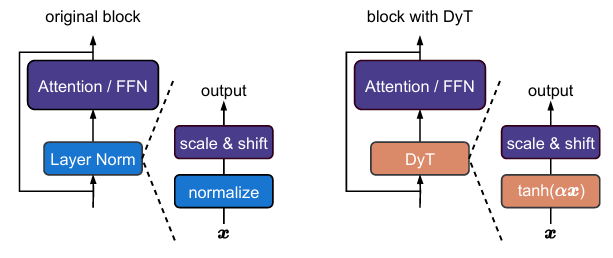
\includegraphics[width=0.5\textwidth]{imagenes/Posibles img/Posición DyT.png}
    \caption{Bloque Transformer original (Izquierda) y propuesta Transformer con DyT (Derecha). DyT reemplaza directamente a LayerNorm sin modificar el resto de la arquitectura \cite{Zhu2025Transformers}.}
    \label{fig:dyt_block}
\end{figure}
 
El parámetro $\alpha$ cumple un rol central. Al escalar la entrada antes de $\tanh$, controla la pendiente efectiva de la curva en $S$: valores grandes de $\alpha$ producen una saturación más rápida, es decir, una curva más abrupta, mientras que valores pequeños producen un comportamiento más lineal en el rango central. Durante el entrenamiento, $\alpha$ aprende a rastrear aproximadamente $1/\sigma$ de las activaciones de entrada, de manera análoga a cómo LayerNorm normaliza por la desviación estándar. Zhu et al. (2025) \cite{Zhu2025Transformers} verifican empíricamente esta correlación: los valores finales de $\alpha$ en redes entrenadas presentan una fuerte correlación positiva con $1/\sigma$ de las activaciones correspondientes.

Para entender por qué $\alpha$ converge a $1/\sigma$, es útil considerar el comportamiento de $\tanh$ en la región lineal. Para valores pequeños de $|\alpha x|$, la función $\tanh$ admite la aproximación de primer orden:

\begin{equation}
\tanh(\alpha x) \approx \alpha x, \qquad |\alpha x| \ll 1
\end{equation}

En esta región, DyT se comporta como una transformación lineal $\boldsymbol{\gamma} \cdot \alpha \mathbf{x} + \boldsymbol{\beta}$, estructuralmente análoga a la parte lineal de LayerNorm con factor de escala efectivo $\alpha$. Si la red aprende a minimizar la discrepancia entre el comportamiento de DyT y el de LayerNorm, el valor óptimo de $\alpha$ en la región central debe satisfacer $\alpha \approx 1/\sigma$, pues ese es el factor de escala que LayerNorm aplica. Fuera de la región lineal, la saturación de $\tanh$ comprime los valores extremos, replicando el efecto de \textit{squashing} de LayerNorm sobre activaciones con varianza alta. Este razonamiento conecta la observación empírica de Zhu et al. con la dinámica de optimización: $\alpha$ converge a $1/\sigma$ porque es el punto de equilibrio que minimiza la diferencia funcional entre DyT y LayerNorm para las activaciones de la red. A diferencia de LayerNorm, donde el factor de escala $1/\sigma$ se recalcula explícitamente en cada pasada hacia adelante a partir de las estadísticas del batch, en DyT este factor emerge de manera implícita como consecuencia del entrenamiento: la red aprende a normalizarse a sí misma sin requerir cómputo de estadísticas, lo que constituye una forma de normalización paramétrica en contraste con la normalización estadística de LayerNorm.

\vspace{0.5cm}
\begin{figure}[htbp]
    \centering
    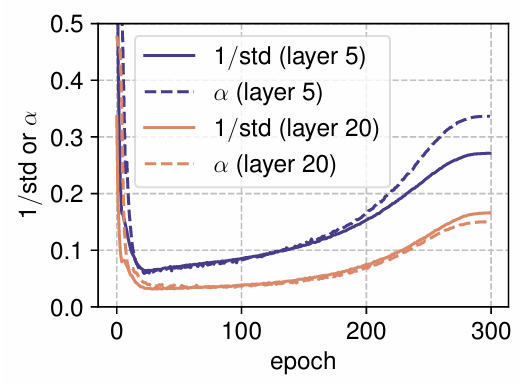
\includegraphics[width=0.4\textwidth]{imagenes/Posibles img/Sigma vs alpha.png}
    \caption{Seguimiento de $1/\sigma$ y $\alpha$ a final de cada época.}
    \label{fig:sigma_vs_alpha}
\end{figure}
 
La inicialización de $\alpha$ es relevante para la estabilidad del entrenamiento. Para modelos no-LLM, Zhu et al. (2025) \cite{Zhu2025Transformers} recomiendan $\alpha_0 = 0{.}5$ como valor por defecto, con $\boldsymbol{\gamma}$ inicializado en $\mathbf{1}$ y $\boldsymbol{\beta}$ en $\mathbf{0}$, en analogía directa con la inicialización estándar de LayerNorm. Con esta configuración, DyT produce curvas de convergencia prácticamente idénticas a las de LN sin necesidad de ajustar ningún otro hiperparámetro del modelo original.
 
\subsection{LayerNorm vs DyT}
 
La diferencia estructural más importante entre LayerNorm y DyT es la ausencia de cálculo de estadísticas en DyT. En LayerNorm, cada pasada hacia adelante requiere calcular $\mu$ y $\sigma^2$ sobre las $C$ dimensiones de cada token, lo que implica una operación de reducción (\textit{reduction}) que introduce dependencias entre elementos del tensor. DyT, al ser completamente elemento a elemento, elimina esta dependencia.
 
Las diferencias funcionales más sustanciales son las siguientes. LayerNorm normaliza \textit{por token}: cada token es escalado por su propia desviación estándar, lo que hace que la transformación sea adaptativa a las estadísticas locales de cada posición temporal. DyT, en cambio, aplica un único escalar global $\alpha$ a todas las posiciones, lo que equivale a una normalización colectiva del tensor completo. Esta distinción es relevante para series temporales con alta variabilidad entre pasos: LayerNorm se adapta localmente a cada paso, mientras que DyT aprende un comportamiento promedio. La segunda diferencia relevante es que LayerNorm centra las activaciones (resta la media), mientras que DyT no lo hace explícitamente. La función $\tanh$ es impar y centrada en cero, lo que introduce un sesgo implícito hacia el centrado, pero sin la garantía de media exactamente cero que provee LayerNorm.

Un aspecto adicional relevante es la elección de la función de \textit{squashing}. Zhu et al. (2025) evalúan alternativas a $\tanh$ en DyT: la función identidad (sin squashing), \textit{hardtanh} y sigmoide. 

\vspace{0.5cm}
\begin{figure}[htbp]
    \centering
    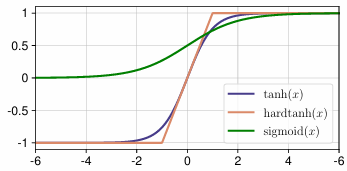
\includegraphics[width=0.4\textwidth]{imagenes/Posibles img/Tanh Hard Sigmoid.png}
    \caption{Curvas de tres funciones squashing: tanh, hardtanh y sigmoide.}
    \label{fig:squashing_functions}
\end{figure}

Los resultados muestran que la ausencia de squashing produce divergencia del entrenamiento, lo que confirma que el efecto de compresión de valores extremos es indispensable. Entre las funciones de squashing, $\tanh$ supera a las demás en rendimiento, lo que los autores atribuyen a dos propiedades: su \textit{suavidad} (es infinitamente diferenciable, a diferencia de \textit{hardtanh} que tiene discontinuidades en la derivada) y su \textit{simetría} respecto al cero (es una función impar, lo que favorece gradientes equilibrados durante el entrenamiento). Estas propiedades hacen que $\tanh$ sea la función de squashing más apta para reemplazar LayerNorm en Transformers.

\vspace{0.5cm}
\begin{figure}[htbp]
    \centering
    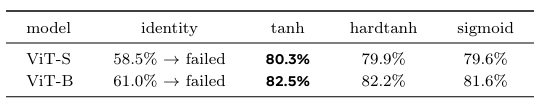
\includegraphics[width=0.5\textwidth]{imagenes/Posibles img/Resultados sigmoid.png}
    \caption{Accuracy de clasificación en ImageNet-1K con diferentes funciones de squashing}
    \label{fig:resultados_squashing_functions}
\end{figure}
 
En términos de rendimiento empírico, Zhu et al. (2025) reportan que DyT iguala o supera a LayerNorm en una amplia variedad de tareas y arquitecturas: clasificación de imágenes, aprendizaje auto-supervisado, modelos de difusión, modelos de lenguaje LLaMA (7B a 70B), habla y secuencias genómicas, entrenados con los mismos hiperparámetros del modelo original con LayerNorm y sin ajuste adicional, lo que respalda su uso como reemplazo directo también en el TFT de este trabajo.

\subsection{Uso de DyT en el TFT para predicción de costos marginales}
 
En el modelo propuesto en este trabajo, DyT reemplaza a LayerNorm en todos los puntos donde esta aparece en la arquitectura TFT: dentro de cada bloque GRN (en la conexión residual final), en las conexiones residuales con compuerta (\textit{gated skip connections}) de la capa LSTM, en la capa de enriquecimiento estático y en la capa de auto-atención interpretable. La sustitución es uniforme y directa: cada ocurrencia de $\text{LayerNorm}(\mathbf{a} + \text{GLU}(\cdot))$ en las ecuaciones de la Sección 2.3.4 se reemplaza por $\text{DyT}(\mathbf{a} + \text{GLU}(\cdot))$, manteniendo inalterada la estructura del bloque.

El parámetro $\alpha$ es independiente para cada capa DyT de la red, lo que significa que el TFT aprende factores de escala distintos para cada GRN, cada conexión residual del LSTM y cada capa de atención. Esta flexibilidad permite que la red calibre el grado de squashing de manera diferenciada según la variabilidad de las activaciones en cada módulo.
 
La motivación principal para adoptar DyT en este contexto es la naturaleza de las series de costo marginal en el Sistema Eléctrico Nacional (SEN). Los costos marginales horarios presentan una distribución fuertemente asimétrica con colas pesadas: en condiciones normales los valores se ubican en el rango de \$20 a \$80 USD/MWh, pero durante eventos de escasez hídrica, fallas de generación o congestiones de transmisión pueden producirse \textit{spikes} que superan los \$300 USD/MWh, valores que exceden en más de un orden de magnitud el rango habitual. En el contexto de la arquitectura TFT, estos valores extremos se propagan como activaciones de gran magnitud a través de los bloques GRN y las capas de atención. LayerNorm los comprime normalizando por la desviación estándar del token correspondiente, pero esta compresión depende de la estadística local de cada paso temporal, lo que puede generar gradientes inestables cuando un token aislado contiene un valor extremo rodeado de valores normales. DyT, al aplicar la saturación de $\tanh$ directamente sobre las activaciones mediante el escalar global $\alpha$, comprime los valores extremos de manera más uniforme e independiente de la estadística local, actuando como una forma de regularización implícita sobre los spikes del costo marginal.

Una segunda consideración es la interacción entre DyT y el mecanismo de atención interpretable del TFT. Dado que los pesos de atención $\tilde{\mathbf{A}}_{ij}$ se calculan sobre representaciones que ya han pasado por la capa de enriquecimiento estático con DyT, la compresión de activaciones extremas garantiza que los scores de atención no sean dominados por spikes temporales, lo que favorece la interpretabilidad: los instantes pasados más relevantes para la predicción reflejan patrones estructurales del mercado eléctrico y no artefactos de valores atípicos.
 
La inicialización de $\alpha$ sigue la recomendación de Zhu et al. (2025) para modelos no-LLM, fijando $\alpha_0 = 0{.}5$ con $\boldsymbol{\gamma} = \mathbf{1}$ y $\boldsymbol{\beta} = \mathbf{0}$. Con esta configuración, el TFT con DyT puede entrenarse directamente con los mismos hiperparámetros utilizados en la versión con LayerNorm, sin requerir ajuste adicional, lo que simplifica el proceso de búsqueda de hiperparámetros y hace la comparación entre ambas versiones directamente interpretable.

En el contexto del modelo híbrido propuesto, la elección de DyT tiene una implicancia adicional que va más allá del rendimiento individual del TFT. Dado que el esquema de Stacking Optimization descrito en la Sección 2.5 combina las predicciones del TFT con LayerNorm, el TFT con DyT y Prophet mediante una combinación lineal con pesos aprendidos, la diversidad entre los modelos base es un factor determinante de la calidad del ensamblaje: modelos que cometen errores distintos y poco correlacionados se complementan mejor que modelos similares. Al reemplazar LayerNorm por DyT se introduce una diferencia estructural en el mecanismo de normalización que, en presencia de spikes del costo marginal, puede producir distribuciones de error cualitativamente distintas entre ambas variantes del TFT. Esta diversidad estructural es precisamente lo que el Stacking Optimization puede explotar para mejorar la predicción conjunta, haciendo de la comparación LayerNorm versus DyT no solo un experimento de ablación sino un componente funcional del modelo híbrido.

\section{Stacking Optimization}

El \textit{Stacking}, también denominado \textit{stacked generalization}, es una técnica de ensamblaje de modelos introducida por Wolpert (1992) \cite{StackingWolpert} que combina las predicciones de múltiples modelos base mediante un metamodelo entrenado para minimizar el error de predicción conjunta. A diferencia de métodos de ensamblaje más simples como el promedio o el voto mayoritario, el Stacking aprende los pesos de combinación de forma supervisada, lo que le permite asignar mayor importancia a los modelos base que presentan menor error en las regiones del espacio de entrada donde los demás fallan.

La intuición central del Stacking es la siguiente: distintos modelos base capturan aspectos complementarios de la distribución de los datos, y el metamodelo puede explotar esta complementariedad combinando sus predicciones de manera que se cancelen los errores individuales. Para que esta cancelación sea efectiva, es necesario que los errores de los modelos base estén escasamente correlacionados, condición que se denomina \textit{diversidad del ensamble} \cite{Dietterich}.

\subsection{Formulación general y diversidad del ensamble}

Sea $\{M_k\}_{k=1}^K$ un conjunto de $K$ modelos base, donde cada modelo $M_k$ produce una predicción $\hat{y}_t^{(k)}$ para el instante $t$, concatenadas en el vector de meta-características $\tilde{\mathbf{z}}_t = (\hat{y}_t^{(1)}, \ldots, \hat{y}_t^{(K)})^\top \in \mathbb{R}^K$. El Stacking, en la forma lineal empleada en este trabajo, combina estas predicciones con pesos $\boldsymbol{\alpha} = (\alpha_1, \ldots, \alpha_K)^\top$:

\begin{equation}
    \hat{y}_t^{\text{stack}} = \sum_{k=1}^{K} \alpha_k\, \hat{y}_t^{(k)} = \boldsymbol{\alpha}^\top \tilde{\mathbf{z}}_t
    \label{eq:stacking_lineal}
\end{equation}

estimados minimizando el error cuadrático medio sobre un conjunto de validación:

\begin{equation}
    \hat{\boldsymbol{\alpha}} = \operatorname*{arg\,min}_{\boldsymbol{\alpha}} \sum_{t \in \mathcal{V}} \left(y_t - \boldsymbol{\alpha}^\top \tilde{\mathbf{z}}_t\right)^2
    \label{eq:stacking_opt}
\end{equation}

donde $\mathcal{V}$ denota el conjunto de índices de validación; en la práctica esta minimización se resuelve mediante métodos analíticos (mínimos cuadrados) o metaheurísticos (Sección 3.5.2).

La ganancia teórica del Stacking sobre cualquiera de los modelos base individuales depende de la diversidad de los errores de predicción. Si $\varepsilon_t^{(k)} = y_t - \hat{y}_t^{(k)}$ denota el error del modelo $k$ en el instante $t$, el error del ensamble es $\varepsilon_t^{\text{stack}} = \sum_{k=1}^K \alpha_k\, \varepsilon_t^{(k)}$ y, asumiendo $\sum_k \alpha_k = 1$, su varianza es:

\begin{equation}
    \text{Var}\!\left(\varepsilon_t^{\text{stack}}\right) = \boldsymbol{\alpha}^\top \boldsymbol{\Sigma}\, \boldsymbol{\alpha}
\end{equation}

donde $\boldsymbol{\Sigma} \in \mathbb{R}^{K \times K}$ es la matriz de covarianzas de los errores, con $\Sigma_{ij} = \text{Cov}(\varepsilon_t^{(i)}, \varepsilon_t^{(j)})$: esta varianza solo se reduce por debajo de la de los modelos base individuales cuando sus errores están poco correlacionados, y no se reduce en absoluto si están perfectamente correlacionados \cite{Dietterich}. Esta observación justifica la importancia de seleccionar modelos base estructuralmente distintos. Cuando los modelos base presentan predicciones muy correlacionadas, la matriz de diseño $\tilde{\mathbf{Z}} = (\tilde{\mathbf{z}}_t)_{t \in \mathcal{V}}$ puede ser casi singular, lo que hace preferible la estimación regularizada mediante regresión de Ridge:

\begin{equation}
    \hat{\boldsymbol{\alpha}} = \left(\tilde{\mathbf{Z}}^\top \tilde{\mathbf{Z}} + \lambda \mathbf{I}\right)^{-1} \tilde{\mathbf{Z}}^\top \mathbf{y}_\mathcal{V}
    \label{eq:stacking_ridge}
\end{equation}

donde $\lambda > 0$ es el parámetro de regularización y $\mathbf{y}_\mathcal{V}$ es el vector de valores observados en el conjunto de validación.

\subsection{Protocolo de entrenamiento y prevención de data leakage}

Un aspecto crítico del Stacking en el contexto de series temporales es la prevención del \textit{data leakage} al construir el conjunto de meta-características. En problemas de clasificación o regresión con datos i.i.d., el procedimiento estándar consiste en generar las predicciones de los modelos base mediante validación cruzada $k$-fold: cada modelo base se entrena en los $k-1$ folds restantes y produce predicciones fuera de muestra para el fold reservado, de modo que las meta-características $\tilde{\mathbf{z}}_t$ son siempre predicciones fuera de muestra \cite{StackingWolpert}. Este protocolo garantiza que el metamodelo se entrena sobre predicciones que no han visto los datos de entrenamiento de los modelos base, evitando sobreajuste.

En series temporales, la validación cruzada estándar no es aplicable porque viola el orden temporal de las observaciones: entrenar con datos futuros para predecir el pasado inflaría artificialmente el rendimiento de los modelos base y produciría meta-características con filtración de información. El protocolo correcto para series temporales es la \textit{validación cruzada con expansión temporal} (\textit{time series split}), ilustrada en la Figura \ref{fig:tss}:

\begin{enumerate}
    \item Se divide la serie en $K+1$ bloques cronológicos de igual tamaño.
    \item En la iteración $k \in \{1, \ldots, K\}$, los modelos base se entrenan sobre los primeros $k$ bloques y producen predicciones fuera de muestra sobre el bloque $k+1$.
    \item Las predicciones fuera de muestra de todos los modelos base para cada observación se concatenan para formar $\tilde{\mathbf{z}}_t$.
    \item El metamodelo se entrena sobre $\{\tilde{\mathbf{z}}_t, y_t\}_{t \in \mathcal{V}}$, donde $\mathcal{V}$ es el conjunto de validación final, cronológicamente posterior al período de entrenamiento de los modelos base.
\end{enumerate}

Este protocolo garantiza que en ningún punto se utilizan observaciones futuras para generar las meta-características, preservando la causalidad temporal del proceso de estimación.

\vspace{0.5cm}
\begin{figure}[htbp]
    \centering
    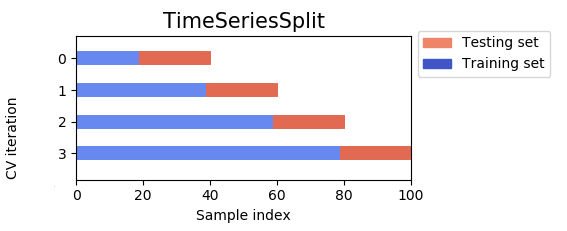
\includegraphics[width=0.5\textwidth]{imagenes/Posibles img/Time Series Split.png}
    \caption{Visualización de Time Series Split.}
    \label{fig:tss}
\end{figure}

El procedimiento de $K$ iteraciones descrito arriba resuelve un problema específico: cuando los modelos base deben reentrenarse en cada fold para que sus predicciones sobre ese fold sean genuinamente fuera de muestra, un único split no basta, porque el conjunto usado para ajustar cada modelo base cambiaría de tamaño y período de un fold a otro si no se repite el ajuste. En el modelo híbrido de este trabajo (Sección 2.5.3), en cambio, cada modelo base --Prophet, $\text{TFT}_\text{LN}$ y $\text{TFT}_\text{DyT}$-- se ajusta una única vez sobre el conjunto de entrenamiento (Sección 3.2), y sus predicciones sobre el conjunto de validación son, por construcción, siempre fuera de muestra: ninguna observación de validación participa del ajuste de ningún modelo base, sin necesidad de repetir el ajuste en múltiples folds para lograrlo. El Stacking Optimization aplicado en este trabajo (Sección 3.5.1) usa, por lo tanto, un único split cronológico train/validación/prueba en lugar de la validación cruzada con expansión temporal de $K$ iteraciones: ambos esquemas evitan la misma fuga de información --que el metamodelo vea predicciones de un modelo base sobre datos que ese modelo ya usó para entrenarse--, pero el split único es suficiente aquí porque esa condición ya se cumple sin necesidad de reajustar los modelos base repetidamente, y evita el costo computacional adicional de entrenar cada modelo base $K$ veces.

\subsection{Stacking Optimization en el modelo híbrido propuesto}

El modelo propuesto en este trabajo dispone de tres predicciones puntuales por barra: Prophet, el TFT con LayerNorm entrenado sobre los residuos de Prophet (denominado $\text{TFT}_\text{LN}$, en su versión de residuos o de precios directos) y el TFT con DyT sobre la serie original (denominado $\text{TFT}_\text{DyT}$). En vez de resolver un único problema de $K=3$ pesos simultáneos como en la formulación general de \eqref{eq:stacking_opt}, el Stacking Optimization aplicado en este trabajo evalúa, para cada barra y cada arquitectura (LN y DyT, por separado), varias combinaciones \textbf{de a lo más dos componentes} a la vez:

\begin{equation}
    \hat{y}_t^{(b),\,\text{Stack}} = w_1^{(b)}\,\hat{y}_t^{(b),\,(1)} + w_2^{(b)}\,\hat{y}_t^{(b),\,(2)}, \qquad w_1^{(b)} + w_2^{(b)} = 1,\;\; w_1^{(b)}, w_2^{(b)} \geq 0
    \label{eq:stacking_hibrido}
\end{equation}

donde el par $\big(\hat{y}^{(1)}, \hat{y}^{(2)}\big)$ instancia una de varias estrategias candidatas --desde un modelo base solo, sin combinar, hasta la combinación de Prophet con la predicción de precios o de residuos del TFT correspondiente-- detalladas junto con sus pesos fijos u optimizados en la Sección 3.5.1. La restricción a dos componentes por combinación, en lugar de una única combinación simultánea de los tres, permite aislar qué par de modelos aporta la mejor combinación por barra, en vez de forzar una única estructura de ensamble para las ocho barras del SEN. Los pesos $(w_1^{(b)}, w_2^{(b)})$ de cada estrategia se estiman por separado para cada barra, minimizando el \textbf{MAE} sobre el conjunto de validación --no el objetivo de mínimos cuadrados de \eqref{eq:stacking_opt}--, dado que el MAE es la métrica de referencia del resto de este trabajo y es más robusto a los \textit{outliers} de cola pesada del costo marginal que el error cuadrático. Al no admitir una solución cerrada como \eqref{eq:stacking_ridge}, la optimización se resuelve con métodos numéricos (búsqueda en grilla, optimización directa, búsqueda aleatoria), descritos junto con la regularización Ridge --incluida como una de las alternativas comparadas, no como el método adoptado-- en la Sección 3.5.2.

La motivación para incluir los tres modelos base como candidatos responde directamente al principio de diversidad discutido en la Sección 2.5.1. Prophet captura la estructura de largo plazo de la serie mediante descomposición aditiva interpretable, pero sus errores son sistemáticos en presencia de fluctuaciones no lineales de corto plazo. El $\text{TFT}_\text{LN}$ modela la variabilidad residual de corto plazo y hereda la estabilidad de LayerNorm frente a secuencias de amplitud moderada. El $\text{TFT}_\text{DyT}$, al operar sobre la serie completa con la compresión de $\tanh$, es más robusto frente a los \textit{spikes} del costo marginal descritos en la Sección 2.4.4, pero puede sobreajustar la tendencia en períodos de baja volatilidad. Esta heterogeneidad estructural en los patrones de error favorece covarianzas $\text{Cov}(\varepsilon^{(i)}, \varepsilon^{(j)})$ pequeñas en magnitud entre cualquier par de modelos base, lo que, por la descomposición de la varianza del ensamble de \eqref{eq:stacking_opt}, respalda que combinar dos de ellos pueda producir ganancias de predicción medibles respecto a cualquiera por separado.

Finalmente, la predicción puntual $\hat{y}_t^{(b),\,\text{Stack}}$ de la mejor estrategia por barra sirve como centro de los intervalos de predicción construidos mediante Conformal Prediction en la Sección 2.6.

\section{Conformal Prediction}

La \textit{Predicción Conforme} o \textit{Conformal Prediction} (CP) es un marco estadístico para construir intervalos de predicción con garantías de cobertura finita sin supuestos distribucionales sobre los datos, más allá de la intercambiabilidad \cite{VovkCP}. A diferencia de los métodos probabilísticos clásicos, cuyas garantías son asintóticas o requieren supuestos paramétricos sobre el modelo, CP produce intervalos válidos para cualquier algoritmo de predicción subyacente, incluyendo redes neuronales, modelos de ensamble y modelos híbridos como el propuesto en este trabajo.

Formalmente, dado un nivel de no-cobertura $\alpha \in (0,1)$ fijado por el usuario, el objetivo es construir un intervalo de predicción $C_{n,\alpha}(x_{n+1})$ tal que:

\begin{equation}
    \mathbb{P}\!\left\{Y_{n+1} \in C_{n,\alpha}(X_{n+1})\right\} \geq 1 - \alpha
    \label{eq:cp_coverage}
\end{equation}

Un intervalo que satisface \eqref{eq:cp_coverage} se denomina \textit{marginalmente válido}. Al mismo tiempo, se exige que el intervalo sea \textit{eficiente}, es decir, lo más estrecho posible: intervalos excesivamente anchos son válidos pero no informativos. El equilibrio entre validez y eficiencia es el criterio central para comparar las distintas variantes de CP \cite{ConformalPrediction}.

La propiedad de intercambiabilidad es el supuesto base de CP: una secuencia aleatoria $(Z_1, \ldots, Z_n)$ es intercambiable si su distribución conjunta es invariante bajo cualquier permutación de los índices. Este supuesto es más débil que la independencia e idéntica distribución (i.i.d.), pero excluye las series temporales, donde la dependencia temporal viola la intercambiabilidad. Esta limitación motiva las variantes adaptativas de CP descritas en las siguientes Secciones.

\subsection{Split Conformal Prediction (SCP)}

La \textit{Split Conformal Prediction} (SCP) es la variante más simple y computacionalmente eficiente de CP, introducida por Papadopoulos et al. (2002) y reformulada por Lei et al. (2018) \cite{LeiCP}. Su idea central es dividir el conjunto de entrenamiento en dos partes: un subconjunto de entrenamiento propio $\mathcal{T}r$ y un conjunto de calibración $\mathcal{C}al$, de modo que el modelo se ajusta solo sobre $\mathcal{T}r$ y los residuos sobre $\mathcal{C}al$ se usan para construir el intervalo.

Dado un modelo de predicción $\hat{\mu}$ ajustado sobre $\mathcal{T}r$, se define la \textit{puntuación de conformidad} (\textit{conformity score}) de cada punto de calibración como el residuo absoluto:

\begin{equation}
    S_i = \left|y_i - \hat{\mu}(x_i)\right|, \quad i \in \mathcal{C}al
    \label{eq:conformity_score}
\end{equation}

El conjunto de puntuaciones de calibración es $\mathcal{S} = \{S_i\}_{i \in \mathcal{C}al} \cup \{+\infty\}$, donde el valor $+\infty$ se añade para garantizar la validez de cobertura en muestra finita. Se calcula el cuantil corregido de nivel $1 - \alpha$ sobre $\mathcal{S}$:

\begin{equation}
    \hat{q}_{1-\alpha}(\mathcal{S}) = \text{Cuantil}\!\left(1 - \alpha;\, \mathcal{S}\right)
    \label{eq:quantile_scp}
\end{equation}

El intervalo de predicción para un nuevo punto $x_{n+1}$ es entonces:

\begin{equation}
    C_{n,\alpha}(x_{n+1}) = \left[\hat{\mu}(x_{n+1}) - \hat{q}_{1-\alpha}(\mathcal{S}),\; \hat{\mu}(x_{n+1}) + \hat{q}_{1-\alpha}(\mathcal{S})\right]
    \label{eq:scp_interval}
\end{equation}

\begin{teorema}[Validez marginal de SCP \cite{LeiCP}]

Si $(X_1, Y_1), \ldots, (X_n, Y_n), (X_{n+1}, Y_{n+1})$ son intercambiables y $\hat{\mu}$ es independiente del conjunto de calibración $\mathcal{C}al$, entonces el intervalo \eqref{eq:scp_interval} satisface:

\begin{equation}
    1 - \alpha \;\leq\; \mathbb{P}\!\left\{Y_{n+1} \in C_{n,\alpha}(X_{n+1})\right\} \;\leq\; 1 - \alpha + \frac{1}{|\mathcal{C}al| + 1}
    \label{eq:scp_validity}
\end{equation}
\end{teorema}

La cota superior en \eqref{eq:scp_validity} muestra que la cobertura excede el nivel nominal en a lo más $\frac{1}{|\mathcal{C}al|+1}$, un término que tiende a cero conforme crece el conjunto de calibración. En la práctica, mantener entre el 10\% y el 30\% del conjunto de entrenamiento para calibración es un compromiso adecuado entre el tamaño del conjunto de calibración y la precisión del modelo ajustado \cite{ConformalPrediction}.

La principal limitación de SCP es que produce intervalos de ancho constante, independiente de las covariables $x_{n+1}$: el cuantil $\hat{q}_{1-\alpha}(\mathcal{S})$ es un escalar global, lo que implica que el intervalo tendrá el mismo ancho para instantes con alta volatilidad que para instantes con precios estables. En el contexto del SEN, donde los spikes del costo marginal concentran la incertidumbre en regímenes específicos, esta rigidez reduce la eficiencia del intervalo. La segunda limitación, más fundamental para series temporales, es que la garantía \eqref{eq:scp_validity} requiere intercambiabilidad, supuesto que no se cumple en datos con dependencia temporal.

\subsection{Regresión Cuantílica Conformada (CQR)}

La \textit{Conformalized Quantile Regression} (CQR), propuesta por Romano et al. (2019) \cite{RomanoCQR}, aborda la limitación de ancho constante de SCP reemplazando el predictor puntual $\hat{\mu}$ por un par de modelos de regresión cuantílica, $\hat{q}_{\alpha/2}$ y $\hat{q}_{1-\alpha/2}$, ajustados de modo que el intervalo se adapte a la covariable $x$ desde el propio modelo base, sin requerir una estimación de escala externa.

Sobre el conjunto de calibración $\mathcal{C}al$, el \textit{score} de conformidad se define como la mayor violación observada de cualquiera de los dos cuantiles:

\begin{equation}
    S_i = \max\left\{\hat{q}_{\alpha/2}(x_i) - y_i,\; y_i - \hat{q}_{1-\alpha/2}(x_i)\right\}, \quad i \in \mathcal{C}al
    \label{eq:cqr_score}
\end{equation}

Un valor positivo de $S_i$ indica que el intervalo cuantílico no cubrió la observación $i$ (por abajo o por arriba); uno negativo indica que la cubrió con margen. El cuantil corregido $\hat{q}_{1-\alpha}(\mathcal{S})$ se calcula sobre estos scores con la misma corrección de muestra finita de \eqref{eq:quantile_scp}, y el intervalo final para un nuevo punto $x_{n+1}$ se obtiene expandiendo los cuantiles estimados en ese margen constante:

\begin{equation}
    C_{n,\alpha}(x_{n+1}) = \left[\hat{q}_{\alpha/2}(x_{n+1}) - \hat{q}_{1-\alpha}(\mathcal{S}),\; \hat{q}_{1-\alpha/2}(x_{n+1}) + \hat{q}_{1-\alpha}(\mathcal{S})\right]
    \label{eq:cqr_interval}
\end{equation}

A diferencia de SCP, donde el ancho del intervalo es un escalar fijo, en CQR el ancho $\hat{q}_{1-\alpha/2}(x) - \hat{q}_{\alpha/2}(x)$ varía con $x$ porque proviene directamente de los modelos cuantílicos; el término $\hat{q}_{1-\alpha}(\mathcal{S})$ solo corrige el sesgo de cobertura de esos cuantiles, preservando la garantía de validez marginal \eqref{eq:scp_validity} bajo el mismo supuesto de intercambiabilidad.

En la implementación utilizada en este trabajo, los modelos de regresión cuantílica son lineales con penalización $\ell_1$ y se ajustan sobre tres variables: la predicción puntual del TFT, $\hat{y}_t$, y las componentes seno y coseno de la hora del día, $\sin(2\pi h_t/24)$ y $\cos(2\pi h_t/24)$, de modo que CQR también incorpora, de forma paramétrica y continua, la heterocedasticidad horaria que motiva a LW Split CP y LW-ACP (Sección \ref{sec:lwacp}). La calibración se realiza mediante validación cruzada de $K$ pliegues sobre el conjunto de validación, sin mezclar el orden temporal (\textit{K-fold cross-conformal}), acumulando los scores de calibración de todos los pliegues antes de calcular $\hat{q}_{1-\alpha}(\mathcal{S})$, lo que evita la inestabilidad observada al calibrar sobre un único split temporal fijo. CQR se emplea en este trabajo como método de comparación externo a la familia de Conformal Prediction, evaluado, al igual que Split CP, ACI y las variantes ponderadas localmente (Sección \ref{sec:lwacp}), sobre las ocho barras del pipeline S+C descrito en el Capítulo 3.

\subsection{Conformal Prediction con Ensemble (EnbPI)}

\textit{Ensemble Prediction Interval} o \textit{EnbPI}, fue propuesto por Xu y Xie (2021) \cite{XuCP} como una adaptación de CP a series temporales mediante \textit{bootstrap} de un ensamble de modelos, cuyos residuos \textit{leave-one-out} se acumulan en una ventana deslizante de \textit{scores} de calibración que se actualiza secuencialmente sin reajustar el modelo subyacente. Xu y Xie (2021) proponen además la variante \textit{EnbPI V2} \cite{ConformalPrediction}, que agrega por media en todas las fases del procedimiento en lugar de mezclar media y cuantil, mejorando la cobertura empírica. Este trabajo no implementa EnbPI: su mecanismo de \textit{bootstrap} está diseñado para un modelo base entrenable con múltiples réplicas, mientras que S+C-LN, la estrategia de referencia adoptada (Sección 4.4.5), es una única predicción del TFT sin ensamble subyacente que bootstrapear.

\subsection{Adaptive Conformal Inference (ACI)}

La \textit{Adaptive Conformal Inference} (ACI) fue propuesta por Gibbs y Candès (2021) \cite{GibbsCP} para adaptarse a series temporales bajo cambios de distribución arbitrarios. La idea central de ACI es reemplazar el nivel de no-cobertura fijo $\alpha$ por un nivel efectivo $\alpha_t$ que se actualiza recursivamente en función del historial de cobertura:

\begin{equation}
    \alpha_{t+1} = \alpha_t + \gamma\left(\alpha - \mathbf{1}\!\left\{y_t \notin C_t(x_t)\right\}\right)
    \label{eq:aci_update}
\end{equation}

donde $\gamma > 0$ es un hiperparámetro de tasa de aprendizaje y $\mathbf{1}\{\cdot\}$ es la función indicadora. La lógica de la actualización \eqref{eq:aci_update} es la siguiente: si en el instante $t$ el intervalo no cubre el valor real ($y_t \notin C_t$), entonces $\alpha_{t+1} < \alpha_t$, lo que amplía el intervalo en la siguiente predicción; si cubre, $\alpha_{t+1} > \alpha_t$, reduciendo el intervalo. Inicialmente se fija $\alpha_1 = \alpha$.

El intervalo de predicción en el instante $t$ se construye con el nivel actualizado:

\begin{equation}
    C_t(x_t) = \left[\hat{\mu}_t(x_t) - \hat{q}_{1-\alpha_t}(\mathcal{S}_{\mathcal{C}al_t}),\; \hat{\mu}_t(x_t) + \hat{q}_{1-\alpha_t}(\mathcal{S}_{\mathcal{C}al_t})\right]
    \label{eq:aci_interval}
\end{equation}

donde $\hat{\mu}_t$ es el modelo reajustado en el instante $t$ sobre los $T_0$ puntos más recientes y $\mathcal{S}_{\mathcal{C}al_t}$ es el conjunto de scores del conjunto de calibración en el instante $t$.

La garantía de cobertura de ACI es asintótica: bajo cualquier distribución de los datos, la frecuencia de no-cobertura converge al nivel nominal \cite{GibbsCP}:

\begin{equation}
    \frac{1}{T_1}\sum_{t=T_0+1}^{T_0+T_1} \mathbf{1}\!\left\{y_t \notin C_t(x_t)\right\} \xrightarrow{a.s.} \alpha, \quad T_1 \to \infty
    \label{eq:aci_asymptotic}
\end{equation}

El parámetro $\gamma$ tiene un impacto crítico sobre la eficiencia de ACI. Zaffran et al. (2022) \cite{ZaffranICML2022} demuestran que en el caso intercambiable, la longitud esperada del intervalo crece linealmente con $\gamma$, mientras que en series con dependencia temporal de tipo AR(1), existe un $\gamma^* > 0$ que minimiza la longitud esperada. Este resultado ilustra el compromiso fundamental de ACI: un $\gamma$ pequeño produce intervalos eficientes cuando los datos son casi intercambiables, pero pierde cobertura cuando la dependencia temporal es fuerte; un $\gamma$ grande garantiza cobertura incluso bajo alta dependencia, pero a costa de generar intervalos ocasionalmente infinitos.

Este compromiso motiva a AgACI (\textit{Aggregated Adaptive Conformal Inference}, Zaffran et al., 2022 \cite{ZaffranICML2022}), una extensión de ACI que evita fijar un único $\gamma$ de antemano: en cada paso, AgACI entrena en paralelo un conjunto de instancias de ACI con distintos valores de $\gamma$ y agrega sus intervalos mediante un esquema de expertos \textit{online} (\textit{Bernstein Online Aggregation}) que pondera cada instancia según su desempeño reciente, heredando garantías de regret acotado de la literatura de agregación de expertos. Es, en ese sentido, el sucesor directo de ACI para el problema específico que este trabajo aborda al fijar $\gamma = 0.05$ de antemano (Sección \ref{sec:aci_metodologia}). Este trabajo no lo implementa por alcance: agregar $\gamma$ mediante expertos introduce un mecanismo adicional (la propia agregación) cuya interacción con la ponderación horaria de LW-ACP no está caracterizada en la literatura, y evaluarla de forma rigurosa, no solo como una variante más, excede el tiempo disponible; queda como comparación externa natural para trabajo futuro, señalada explícitamente aquí en vez de omitirse.

En su formulación original, ACI reajusta el modelo de predicción puntual $\hat{\mu}_t$ en cada instante $t$ sobre una ventana deslizante de observaciones recientes, lo que permite adaptarse a cambios de distribución en el modelo base y no solo en el nivel de cobertura. En este trabajo, en cambio, $\hat{\mu}_t$ es siempre la predicción puntual ya calculada de S+C-LN, fija durante todo el período de prueba: no se reajusta ningún modelo en cada paso, ni el de predicción puntual ni el conjunto de calibración, y el único componente que evoluciona en el tiempo es el nivel $\alpha_t$ (Sección \ref{sec:aci_metodologia}). Esta simplificación, que evita el costo computacional de reentrenar en cada paso, es posible porque S+C-LN no requiere un meta-modelo reentrenable como predictor puntual, a diferencia de formulaciones de ACI sobre un ensamble.

\subsection{CP ponderado localmente: LW Split CP y LW-ACP}
\label{sec:lwacp}

Todas las variantes anteriores comparten una limitación: el cuantil de no conformidad $q$ se calcula sobre un único conjunto de \textit{scores} de calibración, tratando la incertidumbre del modelo como homogénea a lo largo de todo el horizonte de predicción. En el SEN, sin embargo, el error del modelo no es homocedástico en el tiempo: la volatilidad del costo marginal se concentra sistemáticamente en las horas de transición solar (entrada y salida del bloque fotovoltaico), mientras que las horas de mediodía, con generación solar estable, presentan errores sustancialmente menores. Un intervalo de ancho fijo o adaptado únicamente al historial global de errores está necesariamente mal calibrado en algún subconjunto de horas: demasiado ancho cuando la volatilidad es baja, demasiado angosto cuando es alta.

Esta observación motiva la construcción de \textit{scores} de no conformidad \textit{normalizados}, una técnica clásica en la literatura de CP para producir intervalos adaptados a la heterocedasticidad de los datos \cite{VovkCP}. En lugar de calibrar directamente sobre el residuo absoluto $s_t = |y_t - \hat{y}_t|$, se normaliza cada score por una estimación local de la escala del error, $\hat{\sigma}(x_t)$, específica del contexto del punto $t$:

\begin{equation}
    \tilde{s}_t = \frac{|y_t - \hat{y}_t|}{\hat{\sigma}(x_t)}
    \label{eq:lw_score}
\end{equation}

El intervalo resultante, $C_t = [\hat{y}_t - q \cdot \hat{\sigma}(x_t),\; \hat{y}_t + q \cdot \hat{\sigma}(x_t)]$, con $q$ el cuantil de los scores normalizados $\{\tilde{s}_i\}$, se ensancha o contrae proporcionalmente a $\hat{\sigma}(x_t)$, en lugar de mantener un ancho fijo.

Para este trabajo se adopta como variable de contexto la hora del día $h(t) \in \{0, \ldots, 23\}$, dado que es la fuente de heterocedasticidad más sistemática y fácilmente estimable identificada en el análisis de errores del Capítulo 4. La escala local se estima como la desviación estándar de los residuos absolutos de calibración agrupados por hora:

\begin{equation}
    \hat{\sigma}_h = \begin{cases}
        \text{std}\!\left(\{s_i : i \in \mathcal{C}al,\ h(i) = h\}\right) & \text{si } \left|\{i \in \mathcal{C}al : h(i) = h\}\right| \geq 30 \\[4pt]
        \hat{\sigma}_{\text{global}} & \text{en otro caso}
    \end{cases}
    \label{eq:sigma_h}
\end{equation}

donde $\hat{\sigma}_{\text{global}} = \text{std}(\{s_i\}_{i \in \mathcal{C}al})$ actúa como respaldo para horas con pocas observaciones en calibración, evitando estimaciones inestables de $\hat{\sigma}_h$ con muestras pequeñas.

\paragraph{LW Split CP.} La variante \textit{Locally-Weighted Split CP} (LW Split CP) aplica la normalización \eqref{eq:lw_score} con $\hat{\sigma}(x_t) = \hat{\sigma}_{h(t)}$ dentro del esquema de Split CP descrito en la Sección 2.6.1: se calcula un único cuantil $q$ sobre los scores normalizados de calibración, con la misma corrección de muestra finita de \eqref{eq:quantile_scp}, y se reescala por $\hat{\sigma}_{h(t)}$ en cada instante de predicción. El resultado es un intervalo cuyo ancho varía determinísticamente según la hora del día, pero que permanece fijo en el tiempo para una misma hora: es la contraparte localmente ponderada de SCP, sin el componente adaptativo de ACI.

\paragraph{LW-ACP.} La \textit{Locally-Weighted Adaptive Conformal Prediction} (LW-ACP), propuesta en este trabajo como combinación de la ponderación local de \eqref{eq:lw_score}--\eqref{eq:sigma_h} con el mecanismo de adaptación online de ACI \eqref{eq:aci_update}, opera sobre el mismo conjunto de \textit{scores} normalizados de calibración $\{\tilde{s}_i\}_{i \in \mathcal{C}al}$, fijo y calculado una única vez, pero actualiza el nivel de cobertura efectivo $\alpha_t$ en cada paso de la misma forma que ACI online. En cada instante $t$ del conjunto de prueba:

\begin{equation}
    q_t = \hat{Q}_{1-\alpha_t}\!\left(\{\tilde{s}_i\}_{i \in \mathcal{C}al}\right), \qquad
    C_t = \left[\hat{y}_t - q_t\,\hat{\sigma}_{h(t)},\; \hat{y}_t + q_t\,\hat{\sigma}_{h(t)}\right]
    \label{eq:lwacp_interval}
\end{equation}

y $\alpha_{t+1}$ se actualiza según \eqref{eq:aci_update} en función de si $y_t \in C_t$. A diferencia de ACI \textit{online} (Sección 2.6.4), LW-ACP no reajusta el modelo de predicción puntual $\hat{\mu}$ ni el conjunto de calibración en cada paso: el único componente que evoluciona en el tiempo es el nivel $\alpha_t$, aplicado sobre un cuantil que ya incorpora la heterocedasticidad horaria a través de $\hat{\sigma}_{h(t)}$. Esto hace que LW-ACP sea computacionalmente más liviano que ACI online, no requiere reentrenar ningún modelo de meta-aprendizaje, mientras conserva su capacidad de autocorregir la cobertura empírica en línea. La combinación de ambos mecanismos, ponderación local por hora y adaptación online del nivel de cobertura, es el aporte metodológico central de este trabajo en Conformal Prediction, y sus resultados se presentan en la Sección 4.5.

\subsection{Métricas de evaluación de los intervalos de predicción}
\label{sec:metricas_cp}

Para comparar las cuatro variantes de CP implementadas sobre el pipeline S+C (Split CP, ACI, LW Split CP y LW-ACP), más CQR en su rol de método de comparación externo, se utilizan tres métricas complementarias. La primera es la \textit{cobertura empírica}, que mide la proporción de instantes del conjunto de prueba en que el valor real cae dentro del intervalo predicho:

\begin{equation}
    \widehat{\text{Cov}} = \frac{1}{T_1} \sum_{t=T_0+1}^{T_0+T_1} \mathbf{1}\!\left\{y_t \in C_t(x_t)\right\}
    \label{eq:empirical_coverage}
\end{equation}

Un método válido satisface $\widehat{\text{Cov}} \geq 1 - \alpha$ empíricamente. La segunda métrica es la \textit{longitud media del intervalo}:

\begin{equation}
    \bar{L} = \frac{1}{T_1} \sum_{t=T_0+1}^{T_0+T_1} \left|C_t(x_t)\right|
    \label{eq:mean_length}
\end{equation}

donde $|C_t(x_t)|$ denota la longitud del intervalo en el instante $t$. Un método eficiente minimiza $\bar{L}$ sujeto a que $\widehat{\text{Cov}} \geq 1 - \alpha$. La evaluación conjunta de cobertura y longitud media es el criterio estándar adoptado en Zaffran (2024) y permite identificar qué variante de CP ofrece el mejor equilibrio entre validez y eficiencia para la distribución específica de los costos marginales del SEN.

Cobertura y longitud media son, sin embargo, dos métricas separadas: nada impide que un método reduzca la longitud media a costa de fallar por un margen grande en los instantes que no cubre, sin que eso se refleje en $\widehat{\text{Cov}}$, que solo cuenta si el valor real cayó dentro o fuera del intervalo, no cuánto se alejó. El \textit{interval score} o \textit{score} de Winkler combina ambas dimensiones en una única cifra, penalizando la longitud del intervalo y, adicionalmente, la magnitud de la violación cuando el valor real queda fuera de él:

\begin{equation}
    IS_t(\alpha) = \left|C_t(x_t)\right| + \frac{2}{\alpha}\left(l_t - y_t\right)\mathbf{1}\{y_t < l_t\} + \frac{2}{\alpha}\left(y_t - u_t\right)\mathbf{1}\{y_t > u_t\}
    \label{eq:winkler_score}
\end{equation}

donde $C_t(x_t) = [l_t, u_t]$. Un intervalo que cubre $y_t$ solo aporta su longitud al puntaje; uno que no cubre suma además una penalización proporcional a la distancia entre $y_t$ y el límite violado, escalada por $2/\alpha$ para que la penalización sea comparable en magnitud al costo de ensanchar el intervalo lo suficiente como para haber evitado esa falla. Un puntaje de Winkler medio más bajo indica un mejor equilibrio conjunto entre eficiencia y calibración que comparar ancho y cobertura por separado, precisamente porque no permite que una mejora en una dimensión oculte un deterioro en la otra.
\chapter{Metodología}

\section{Datos}

\subsection{Fuente y descripción}

Los datos utilizados en este trabajo provienen del portal del Coordinador Eléctrico Nacional (CEN) de Chile. La variable objetivo es el costo marginal horario en ocho barras de 220 kV del sistema, cubriendo el período comprendido entre enero de 2020 y abril de 2026, lo que representa aproximadamente 55.000 observaciones por barra. Las ocho barras consideradas son Atacama, Cardones, Charrúa, Crucero, Pan de Azúcar, Puerto Montt, Quillota y Tarapacá, seleccionadas por su representatividad geográfica a lo largo del sistema: las barras del norte, Atacama, Cardones, Crucero, Pan de Azúcar y Tarapacá, concentran la generación solar del desierto de Atacama y la región de Antofagasta, y la generación eólica de la región de Coquimbo; la barra de Quillota, cercana a Valparaíso, refleja la demanda industrial y residencial de la zona central, y las barras del sur, Charrúa y Puerto Montt, capturan la dinámica de la generación hidroeléctrica de la zona centro-sur y sur del sistema. Esta distribución geográfica introduce heterogeneidad estructural entre barras, especialmente en episodios de congestión de transmisión donde los precios se desacoplan, lo que justifica la decisión de entrenar modelos independientes por barra descrita en la Sección 2.1.

El período 2020--2026 es especialmente relevante para el problema de forecasting porque concentra dos fenómenos estructurales de alto impacto en el SEN: la aceleración de la penetración de energías renovables no convencionales, que llevó la participación ERNC del 20\% al 40\% de la generación total, y los episodios de sobreoferta solar que generaron curtailments récord a partir de 2023. Ambos fenómenos introducen cambios estructurales graduales en la distribución del costo marginal que constituyen el principal desafío metodológico del problema.

\subsection{Estadísticas descriptivas y análisis exploratorio}

La Figura \ref{fig:series_barras} presenta las series de costo marginal horario para las ocho barras durante el período de estudio.

\begin{figure}[htbp]
    \centering
    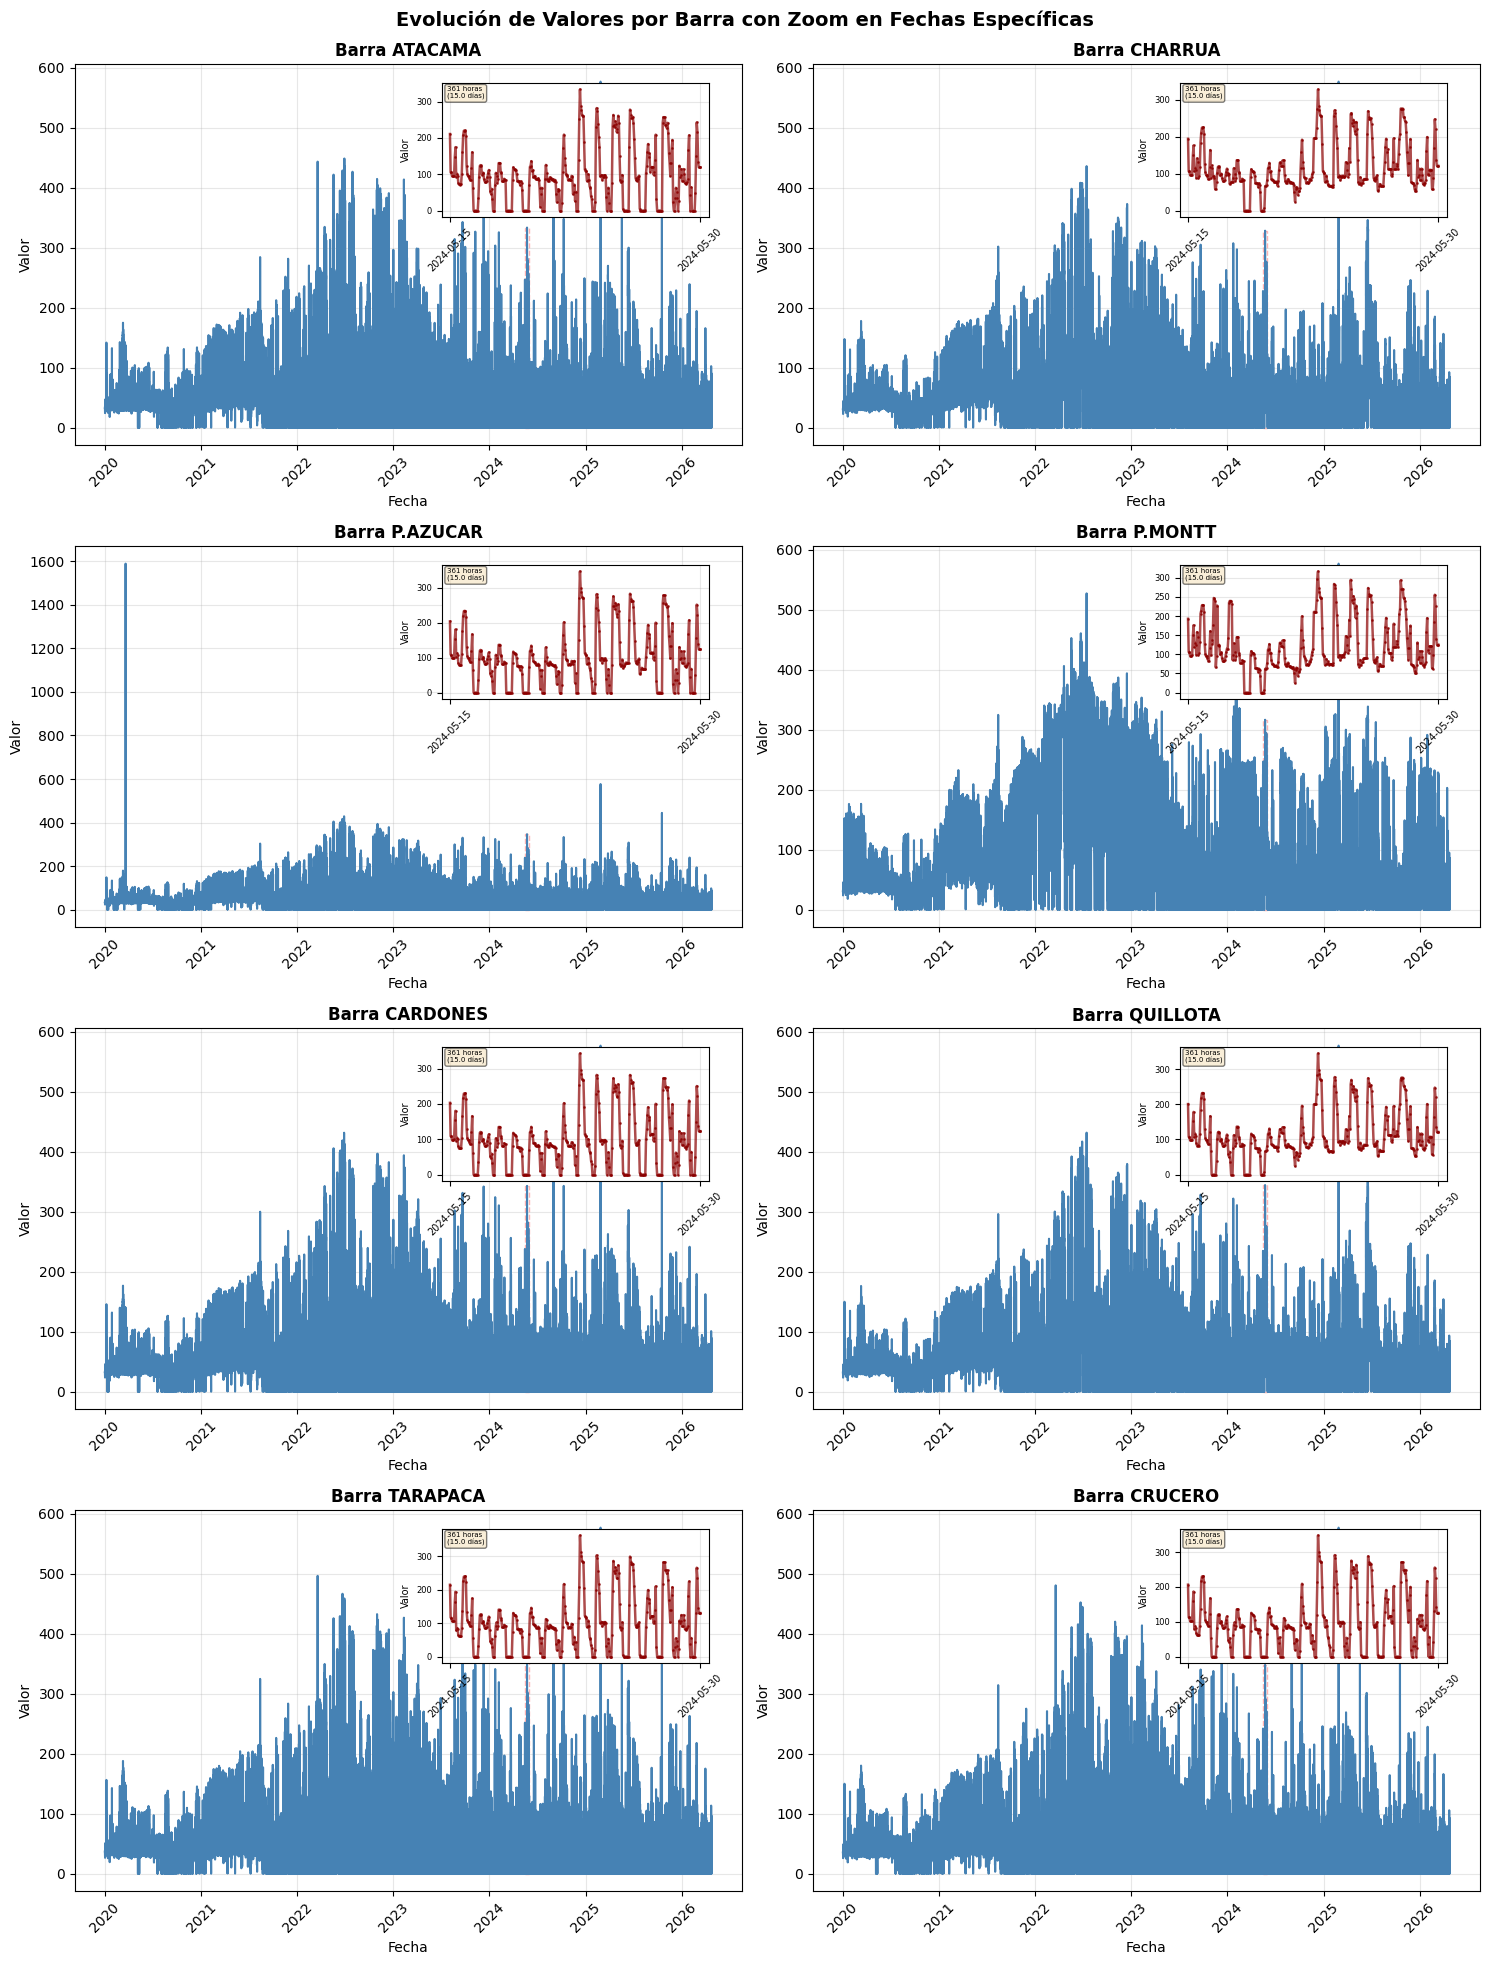
\includegraphics[width=0.9\linewidth]{imagenes/Posibles img/Serie Barras.png}
    \caption{Evolución del costo marginal horario para las ocho barras del SEN, período 2020--2026. Zoom en el período del 15/05/2024 - 30/05/2024}
    \label{fig:series_barras}
\end{figure}

Las series exhiben tres características estructurales relevantes. En primer lugar, presentan estacionalidad múltiple visible sobre todo a escala diaria y semanal, con un ciclo diario marcado por la caída del costo marginal durante el bloque solar y el alza en horas de menor radiación. En segundo lugar, se observan spikes de alta magnitud asociados a eventos de escasez hídrica, fallas de generación o congestiones de transmisión. En tercer lugar, se aprecia una tendencia decreciente en el nivel base del costo marginal a partir de 2022 en las barras del norte, consistente con la incorporación masiva de capacidad solar en esa zona del sistema.

La Tabla \ref{tab:estadisticas} resume las estadísticas descriptivas de cada barra. La heterogeneidad entre barras es marcada. Puerto Montt presenta la media más alta con 100.11 USD/MWh y la mayor desviación estándar con 94.05 USD/MWh, muy superior al resto de las barras, lo que refleja la influencia de la generación hidroeléctrica y su mayor variabilidad estacional asociada a los ciclos de precipitaciones. Las barras del norte, en cambio, presentan medias más bajas y medianas en el rango de \$54 a \$57 USD/MWh, coherente con la abundante generación solar que presiona el costo marginal hacia abajo durante el bloque diurno. El mínimo de 0.0 USD/MWh es común a todas las barras y corresponde a episodios de sobreoferta renovable donde el costo marginal colapsa. El caso más notable es la barra Pan de Azúcar, que registra un máximo de 1588.95 USD/MWh, considerablemente superior al máximo de 576.82 USD/MWh compartido por las demás barras, lo que refleja un evento extremo de congestión o escasez ocurrido cerca del año 2020, visible en la Figura \ref{fig:series_barras}. Este spike de magnitud excepcional constituye precisamente el tipo de evento que motiva el uso de DyT en la arquitectura TFT, por su capacidad de comprimir activaciones extremas de manera más robusta que LayerNorm, como se argumentó en la Sección 2.4.5.

\begin{table}[htbp]
    \centering
    \begin{tabular}{lrrrrr}
        \toprule
        Barra & Media & Desv. Est. & Mínimo & Mediana & Máximo \\
        \midrule
        Atacama       & 62.30  & 60.20 & 0.0 & 55.14 & 576.82   \\
        Cardones      & 62.37  & 59.75 & 0.0 & 55.01 & 576.82   \\
        Charrúa       & 66.21  & 58.87 & 0.0 & 57.35 & 576.82   \\
        Crucero       & 63.23  & 61.79 & 0.0 & 54.36 & 576.82   \\
        Pan de Azúcar & 63.26  & 60.32 & 0.0 & 56.40 & 1588.95 \\
        Puerto Montt  & 100.11 & 94.05 & 0.0 & 67.14 & 576.82   \\
        Quillota      & 66.74  & 58.79 & 0.0 & 59.09 & 576.82   \\
        Tarapacá      & 65.28  & 64.08 & 0.0 & 56.03 & 576.82   \\
        \bottomrule
    \end{tabular}
    \caption{Estadísticas descriptivas del costo marginal horario para las ocho barras del SEN, período 2020--2026.}
    \label{tab:estadisticas}
\end{table}

\subsection{Análisis de estacionariedad}

Para caracterizar formalmente las propiedades estadísticas de cada serie se aplican conjuntamente las pruebas ADF y KPSS descritas en la Sección 2.1.1. Los resultados se presentan en la Tabla \ref{tab:estacionariedad}.

\begin{table}[htbp]
    \centering
    \begin{tabular}{lcccc}
        \toprule
        Barra & Est. ADF & $p$-valor ADF & Est. KPSS & $p$-valor KPSS \\
        \midrule
        Atacama       & $-$13.2000 & $<0.001$ & 8.1252 & $<0.01$ \\
        Cardones      & $-$12.4464 & $<0.001$ & 8.1567 & $<0.01$ \\
        Charrúa       & $-$12.7728 & $<0.001$ & 8.4554 & $<0.01$ \\
        Crucero       & $-$12.6482 & $<0.001$ & 4.5352 & $<0.01$ \\
        Pan de Azúcar & $-$12.6063 & $<0.001$ & 7.2476 & $<0.01$ \\
        Puerto Montt  & $-$11.6217 & $<0.001$ & 4.8858 & $<0.01$ \\
        Quillota      & $-$12.7277 & $<0.001$ & 4.5890 & $<0.01$ \\
        Tarapacá      & $-$12.8396 & $<0.001$ & 8.2951 & $<0.01$ \\
        \bottomrule
    \end{tabular}
    \caption{Resultados de las pruebas de estacionariedad ADF y KPSS para las ocho barras.}
    \label{tab:estacionariedad}
\end{table}

El patrón es consistente en todas las barras: la prueba ADF rechaza la hipótesis nula de raíz unitaria con $p < 0.001$, evidencia de que las series no son paseos aleatorios puros y exhiben reversión a la media en el largo plazo. La prueba KPSS, en cambio, rechaza su hipótesis nula de estacionariedad en sentido débil con $p < 0.01$ (reportado en su valor límite inferior, dado que los estadísticos superan ampliamente los umbrales críticos de la librería). Esta combinación --rechazo simultáneo de ambas hipótesis nulas-- no es contradictoria, sino un patrón conocido en presencia de quiebres estructurales: el estadístico KPSS asume una serie que fluctúa en torno a un nivel (o tendencia) determinístico fijo, y tiende a rechazar la estacionariedad incluso cuando no existe una raíz unitaria genuina si ese nivel se desplaza gradualmente en el tiempo, como es esperable dada la incorporación continua de capacidad renovable al SEN durante el período de datos (Sección 3.1). En conjunto, ambas pruebas son consistentes con series que revierten a la media en el largo plazo (sin raíz unitaria, según ADF) pero cuyo nivel base no es fijo sino que se desplaza gradualmente (lo que basta para que KPSS rechace la estacionariedad, sin que esto implique nada directamente sobre la varianza de la serie). Esta caracterización, centrada en el nivel de la serie más que en su varianza, justifica específicamente el uso de Prophet con detección automática de puntos de quiebre, que modela explícitamente esos desplazamientos graduales de nivel. La heterocedasticidad asociada a los \textit{spikes} de alta magnitud, visible en las estadísticas descriptivas de la Tabla \ref{tab:estadisticas}, es una propiedad adicional de la serie --no algo que ADF o KPSS, ambas centradas en la dinámica del nivel, permitan concluir por sí solas-- y es la que motiva, de forma independiente, la estandarización z-score como transformación de preprocesamiento.

\section{Preprocesamiento}

El preprocesamiento de los datos se realiza en dos etapas diferenciadas según el modelo destino, dado que Prophet y el TFT tienen requisitos distintos respecto a la escala de los datos.

\subsection{Limpieza y tratamiento de valores atípicos}

En primer lugar se verifica la integridad de la serie temporal. Los datos del CEN no presentan valores faltantes en el período estudiado; no obstante, el pipeline contempla interpolación lineal como mecanismo de contingencia ante eventuales ausencias puntuales, preservando así la continuidad temporal de la serie sin introducir sesgos hacia valores futuros.

En segundo lugar se tratan los outliers. Dado que las series de costo marginal presentan spikes de alta magnitud asociados a eventos excepcionales, se aplica un umbral de 4 desviaciones estándar calculadas sobre el conjunto de entrenamiento: las observaciones que superan $\hat{\mu} + 4\hat{\sigma}$ se reemplazan mediante interpolación lineal entre los valores adyacentes. Este umbral es suficientemente amplio para preservar los spikes estructurales del mercado, como los episodios de escasez hídrica o congestión de transmisión, que son parte de la dinámica real del sistema y deben ser aprendidos por el modelo, mientras elimina únicamente los valores de magnitud excepcional que podrían distorsionar el entrenamiento, como el spike de 1.588,95 USD/MWh registrado en la barra Pan de Azúcar. El umbral se estima exclusivamente sobre el conjunto de entrenamiento y se aplica sin reestimación al resto de los conjuntos, evitando data leakage.

\subsection{División temporal de los datos}

Los datos se dividen en tres conjuntos cronológicamente ordenados, respetando estrictamente la causalidad temporal: ningún conjunto contiene observaciones posteriores a las del conjunto siguiente. La división adoptada es 70\% entrenamiento, 15\% validación y 15\% test, que corresponde a los siguientes períodos:

\begin{table}[htbp]
    \centering
    \begin{tabular}{llll}
        \toprule
        Conjunto & Inicio & Término & Proporción \\
        \midrule
        Entrenamiento & 2020-01-01 01:00 & 2024-06-01 12:00 & 70\% \\
        Validación    & 2024-06-01 13:00 & 2025-05-13 06:00 & 15\% \\
        Test          & 2025-05-13 07:00 & 2026-04-24 00:00 & 15\% \\
        \bottomrule
    \end{tabular}
    \caption{División temporal de los datos por conjunto.}
    \label{tab:division}
\end{table}

El conjunto de entrenamiento cubre el período 2020--2024, que incluye la transición energética acelerada y los episodios de sobreoferta solar de los primeros años. El conjunto de validación, comprendido entre junio de 2024 y mayo de 2025, se utiliza para la optimización de hiperparámetros de Prophet, la selección del mejor ensamble en el Stacking Optimization y el ajuste de los pesos de combinación. El conjunto de prueba, de mayo de 2025 a abril de 2026, se reserva exclusivamente para la evaluación final del modelo y la construcción de los intervalos de Conformal Prediction, y no es accedido en ninguna etapa del entrenamiento ni de la selección de modelos.

\subsection{Normalización}

La normalización se aplica de manera diferenciada según el modelo. Prophet opera directamente sobre los valores originales del costo marginal en USD/MWh, dado que su formulación aditiva es interpretable en la escala original y sus componentes de tendencia y estacionalidad tienen significado físico directo en esa escala.

Para el TFT, en cambio, se aplica estandarización z-score independientemente para cada barra:

\begin{equation}
    \tilde{y}_t^{(b)} = \frac{y_t^{(b)} - \hat{\mu}^{(b)}}{\hat{\sigma}^{(b)}}
\end{equation}

donde $\hat{\mu}^{(b)}$ y $\hat{\sigma}^{(b)}$ son la media y desviación estándar estimadas exclusivamente sobre el conjunto de entrenamiento de la barra $b$. La normalización independiente por barra es necesaria porque las series presentan niveles y variabilidades distintas, como se evidencia en la Tabla \ref{tab:estadisticas}, donde Puerto Montt tiene una media de 100.11 USD/MWh frente a las barras del norte con medias en torno a 62--66 USD/MWh. Aplicar una normalización conjunta introduciría un sesgo sistemático en las barras con niveles más extremos. Los parámetros $\hat{\mu}^{(b)}$ y $\hat{\sigma}^{(b)}$ se aplican sin reestimación a los conjuntos de validación y prueba, preservando la integridad de la evaluación fuera de muestra.

\section{Modelo Prophet}

\subsection{Configuración y optimización de hiperparámetros}

Prophet se entrena sin transformación previa, sobre los valores originales del costo marginal en USD/MWh (Sección 3.2.3). Se incorporan los feriados nacionales del calendario chileno como variable exógena mediante el argumento \texttt{holidays}, capturando el efecto sistemático de los días festivos sobre el despacho del SEN descrito en la Sección 2.2.3. Las estacionalidades diaria, semanal y anual se activan explícitamente. El tipo de tendencia se fija como lineal por tramos (\texttt{growth='linear'}), adecuado para series de precios que no tienen una capacidad de saturación definida. Además, esta decisión de diseño está motivada por las dificultades prácticas en la implementación del modo multiplicativo: Prophet requiere la especificación explícita de valores de techo y piso para ese modo, parámetros que no tienen una interpretación directa en series de costos marginales sin capacidad de saturación definida, y el entrenamiento con modo multiplicativo presentó tiempos de cómputo significativamente mayores sin mejoras observables en validación preliminar. La búsqueda se realiza mediante grid search minimizando el MAE sobre el conjunto de validación, preservando la causalidad temporal.

Los hiperparámetros optimizados son \texttt{changepoint\_prior\_scale} (CPS), que controla la flexibilidad de la tendencia lineal por tramos, y \texttt{seasonality\_prior\_scale} (SPS), que controla la flexibilidad de las componentes estacionales, ambos descritos en la Sección 2.2. La Tabla~\ref{tab:prophet_params} presenta los hiperparámetros óptimos encontrados para cada barra.

\begin{table}[htbp]
    \centering
    \begin{tabular}{lccc}
        \toprule
        Barra & CPS & SPS & MAE val. \\
        \midrule
        Atacama       & 0.02 & 0.2   & 21.54 \\
        Cardones      & 0.05 & 5.0   & 21.89 \\
        Charrúa       & 0.02 & 0.01  & 24.30 \\
        Crucero       & 0.05 & 0.007 & 22.25 \\
        Pan de Azúcar & 0.05 & 0.007 & 22.66 \\
        Puerto Montt  & 0.05 & 0.01  & 46.01 \\
        Quillota      & 0.02 & 1.0   & 23.77 \\
        Tarapacá      & 0.05 & 0.01  & 23.09 \\
        \bottomrule
    \end{tabular}
    \vspace{0.2cm}
    \caption{Hiperparámetros óptimos de Prophet por barra. MAE en conjunto de validación (USD/MWh).}
    \label{tab:prophet_params}
\end{table}

Dos patrones emergen de los resultados. Primero, los valores de CPS son bajos en todas las barras (0.02--0.05), indicando que Prophet prefiere tendencias suaves con pocos cambios abruptos, consistente con los cambios estructurales graduales del mercado descritos en la Sección 3.1. Segundo, los valores de SPS son notablemente bajos en la mayoría de las barras (0.007--0.01), lo que indica que con datos horarios Prophet prefiere estacionalidades rígidas, posiblemente porque la alta densidad temporal de las observaciones ya provee suficiente información para estimar los patrones estacionales sin necesidad de flexibilidad adicional. Las excepciones son Cardones (SPS=5.0) y Quillota (SPS=1.0), cuyas estacionalidades requieren mayor adaptabilidad, y Atacama (SPS=0.2), que ocupa una posición intermedia.

\subsection{Componentes de tendencia y estacionalidad anual}

La Figura \ref{fig:prophet_trend_yearly} presenta las componentes de tendencia y de estacionalidad anual estimadas por Prophet para las ocho barras, período 2020--2026.

\begin{figure}[htbp]
    \centering
    \begin{minipage}[t]{0.48\textwidth}
        \centering
        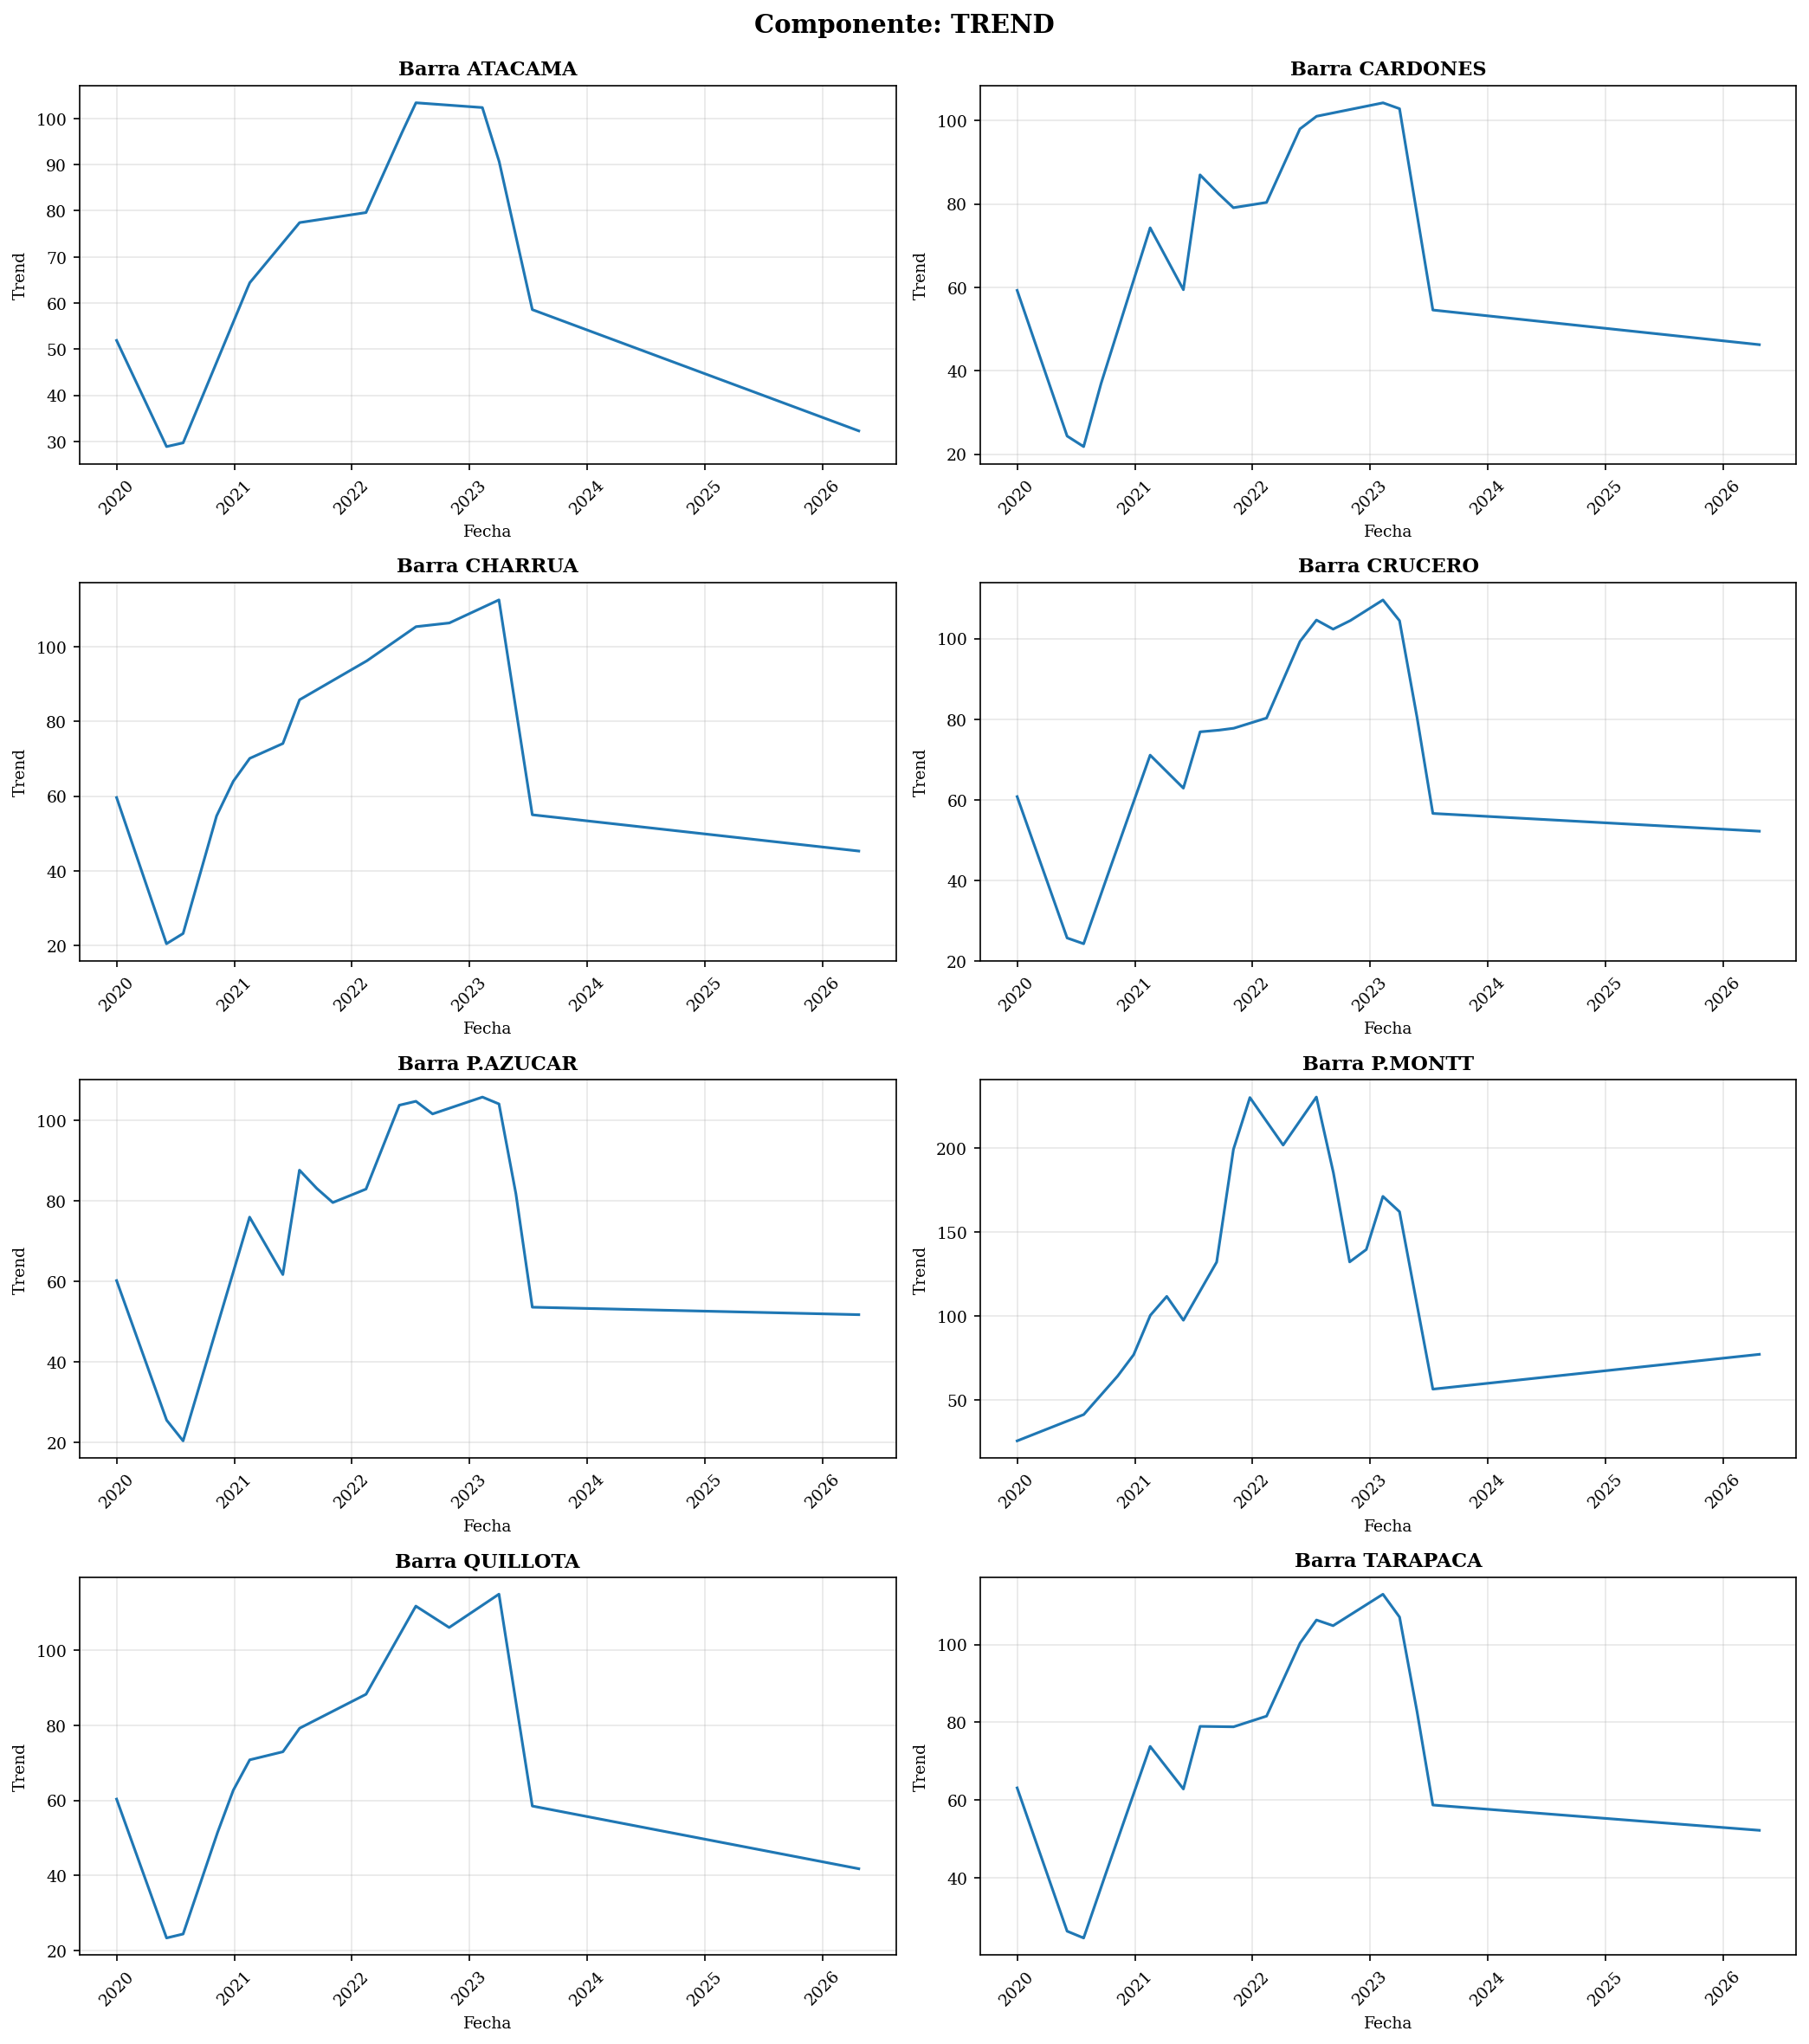
\includegraphics[width=\textwidth]{imagenes/Posibles img/Componente Trend.png}
        \caption*{Tendencia}
    \end{minipage}
    \hfill
    \begin{minipage}[t]{0.48\textwidth}
        \centering
        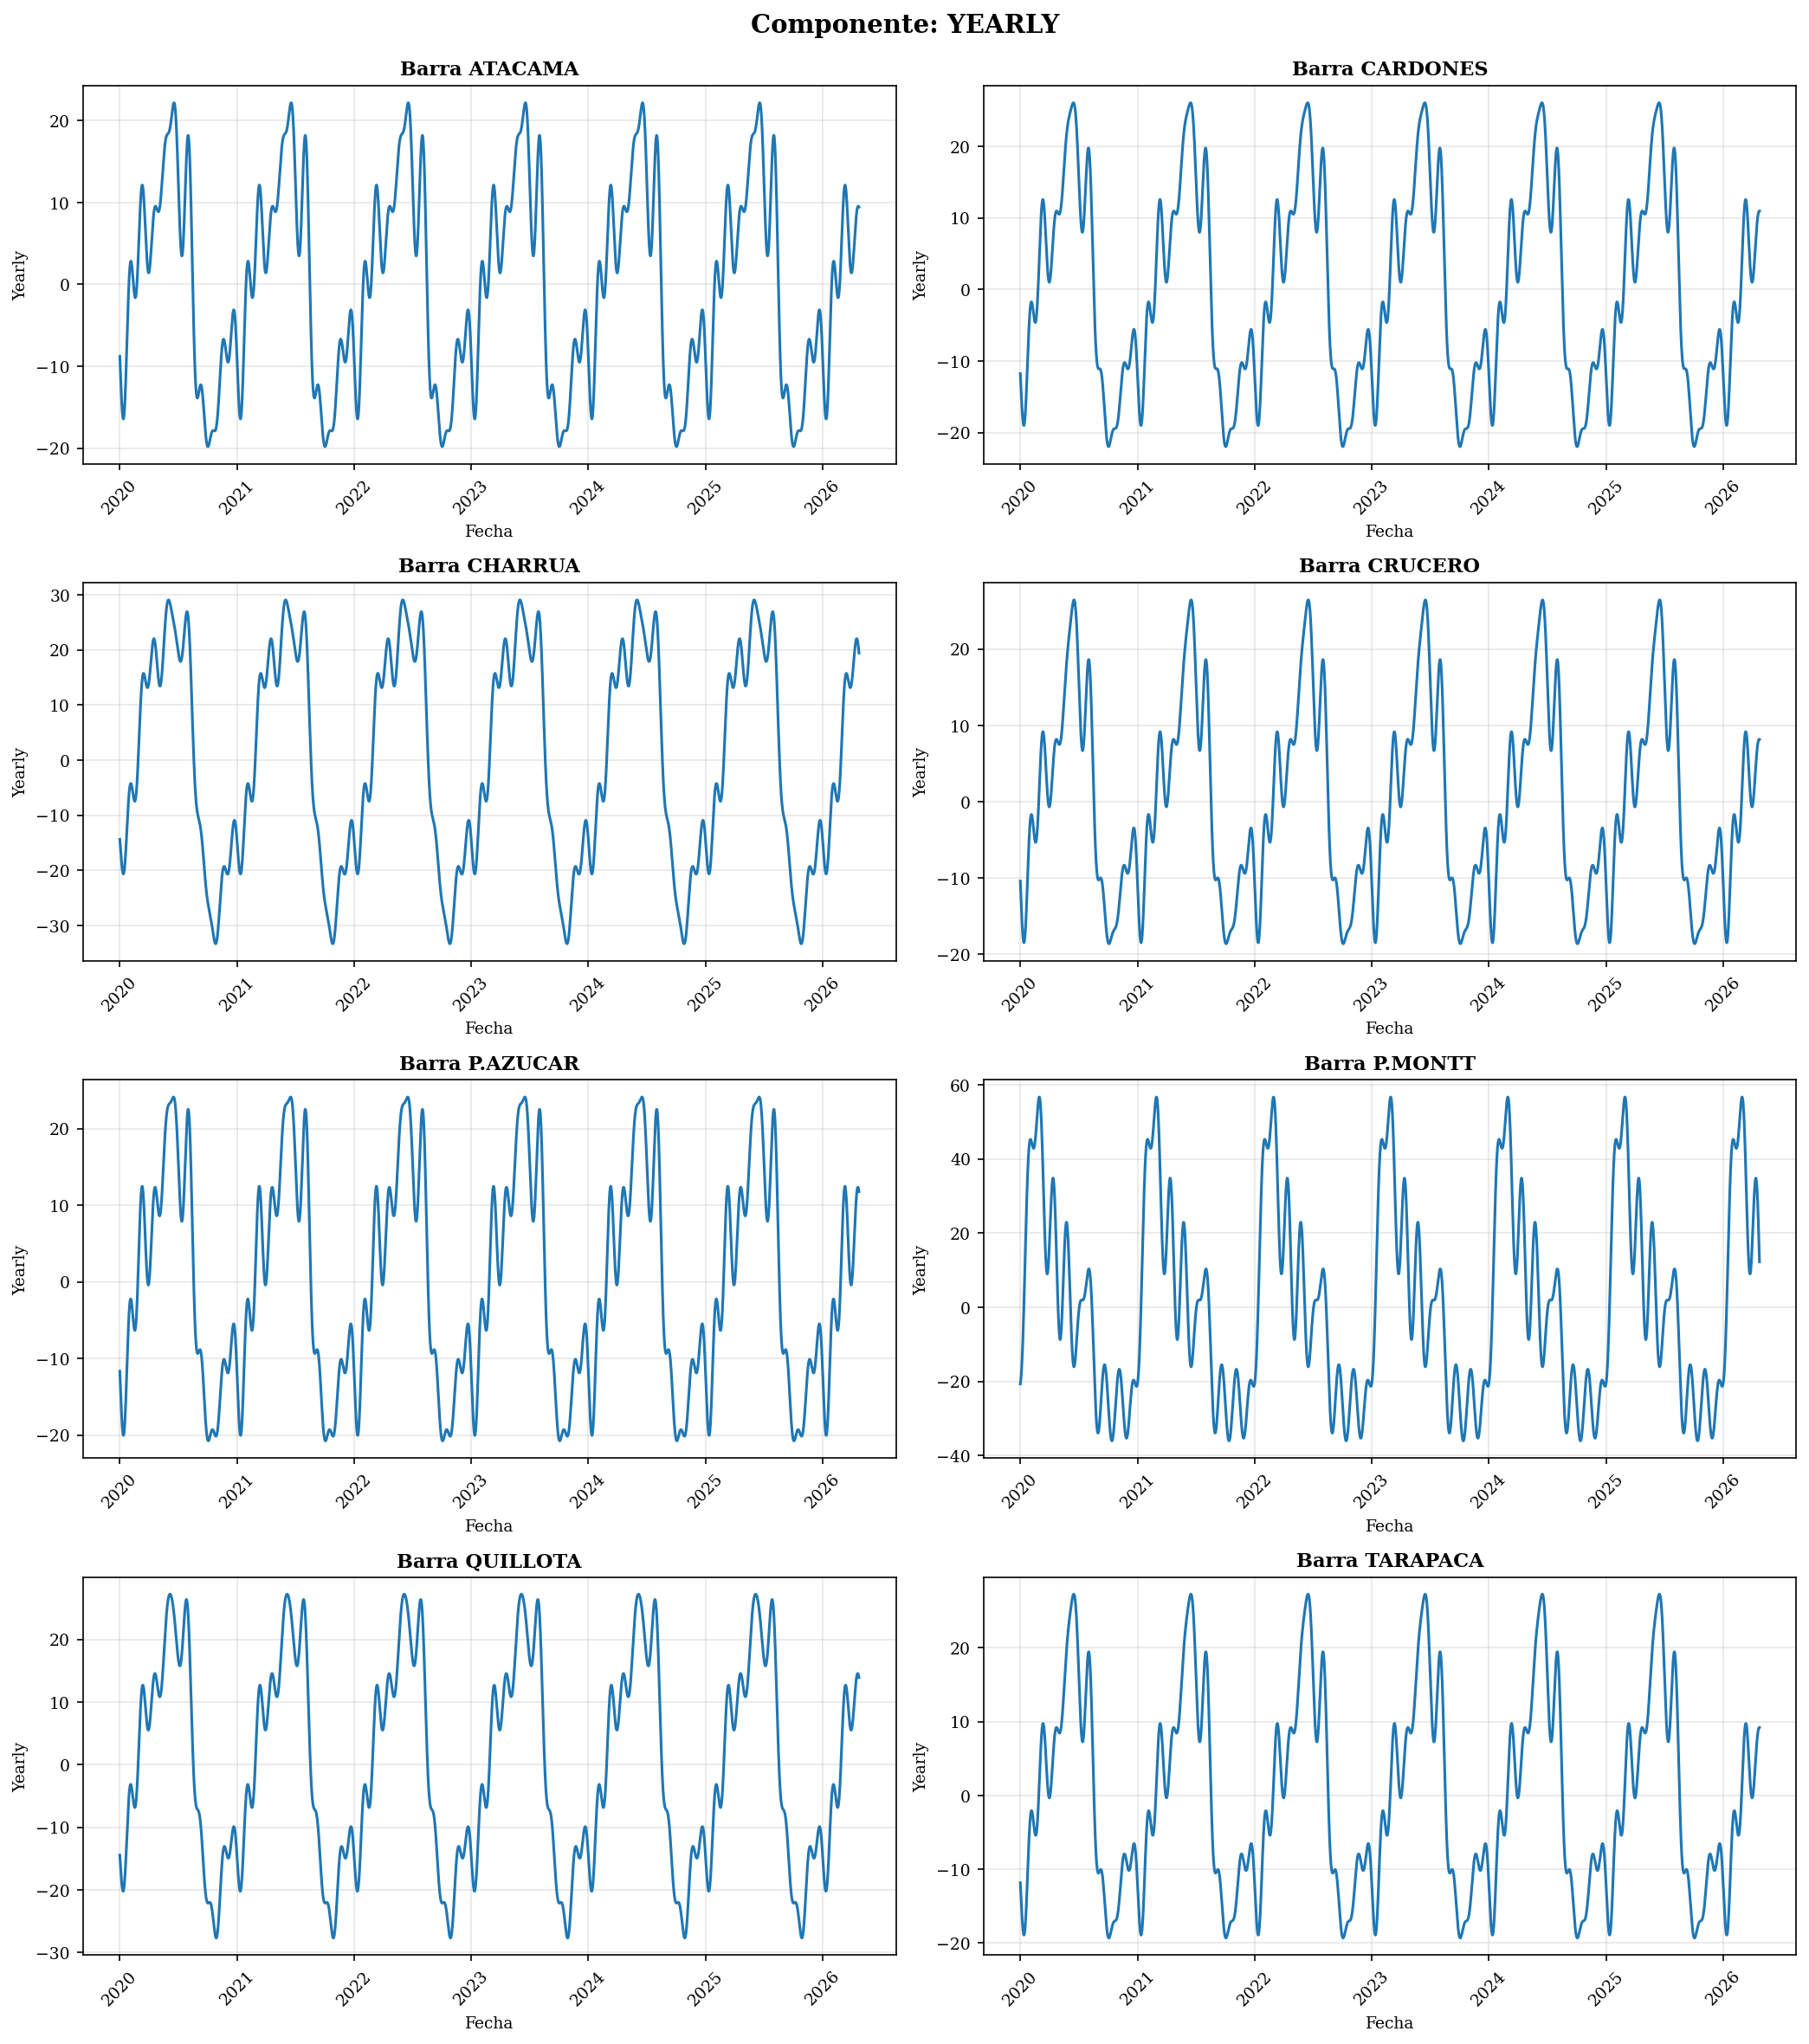
\includegraphics[width=\textwidth]{imagenes/Posibles img/Componente Yearly.png}
        \caption*{Estacionalidad anual}
    \end{minipage}
    \caption{Componentes de tendencia y de estacionalidad anual estimadas por Prophet para las ocho barras del SEN, período 2020--2026.}
    \label{fig:prophet_trend_yearly}
\end{figure}

La tendencia revela un patrón común a todas las barras: una fase de alza sostenida entre 2020 y 2022--2023, consistente con la recuperación post-pandemia y la alta demanda de ese período, seguida de una caída pronunciada desde 2024 que refleja la incorporación masiva de capacidad solar y eólica. La componente anual, por su parte, muestra una amplitud moderada de $\pm$20--30 USD/MWh en las barras del norte, asociada al ciclo estacional de la radiación solar. Puerto Montt es la excepción en ambas componentes: una tendencia con niveles muy superiores (en torno a 200 USD/MWh en el peak de 2022--2023) y una caída más abrupta, y la mayor amplitud anual del grupo ($\pm$60 USD/MWh), consistentes con la dependencia de los ciclos hidrológicos de deshielo y precipitaciones que rigen la generación hidroeléctrica del sur.

\subsection{Predicciones a 48 horas}

La Figura \ref{fig:prophet_pred48} ilustra las predicciones de Prophet para un horizonte de 48 horas a partir del último instante del conjunto de prueba, mostrando el histórico reciente y la proyección para cada barra.

\begin{figure}[htbp]
    \centering
    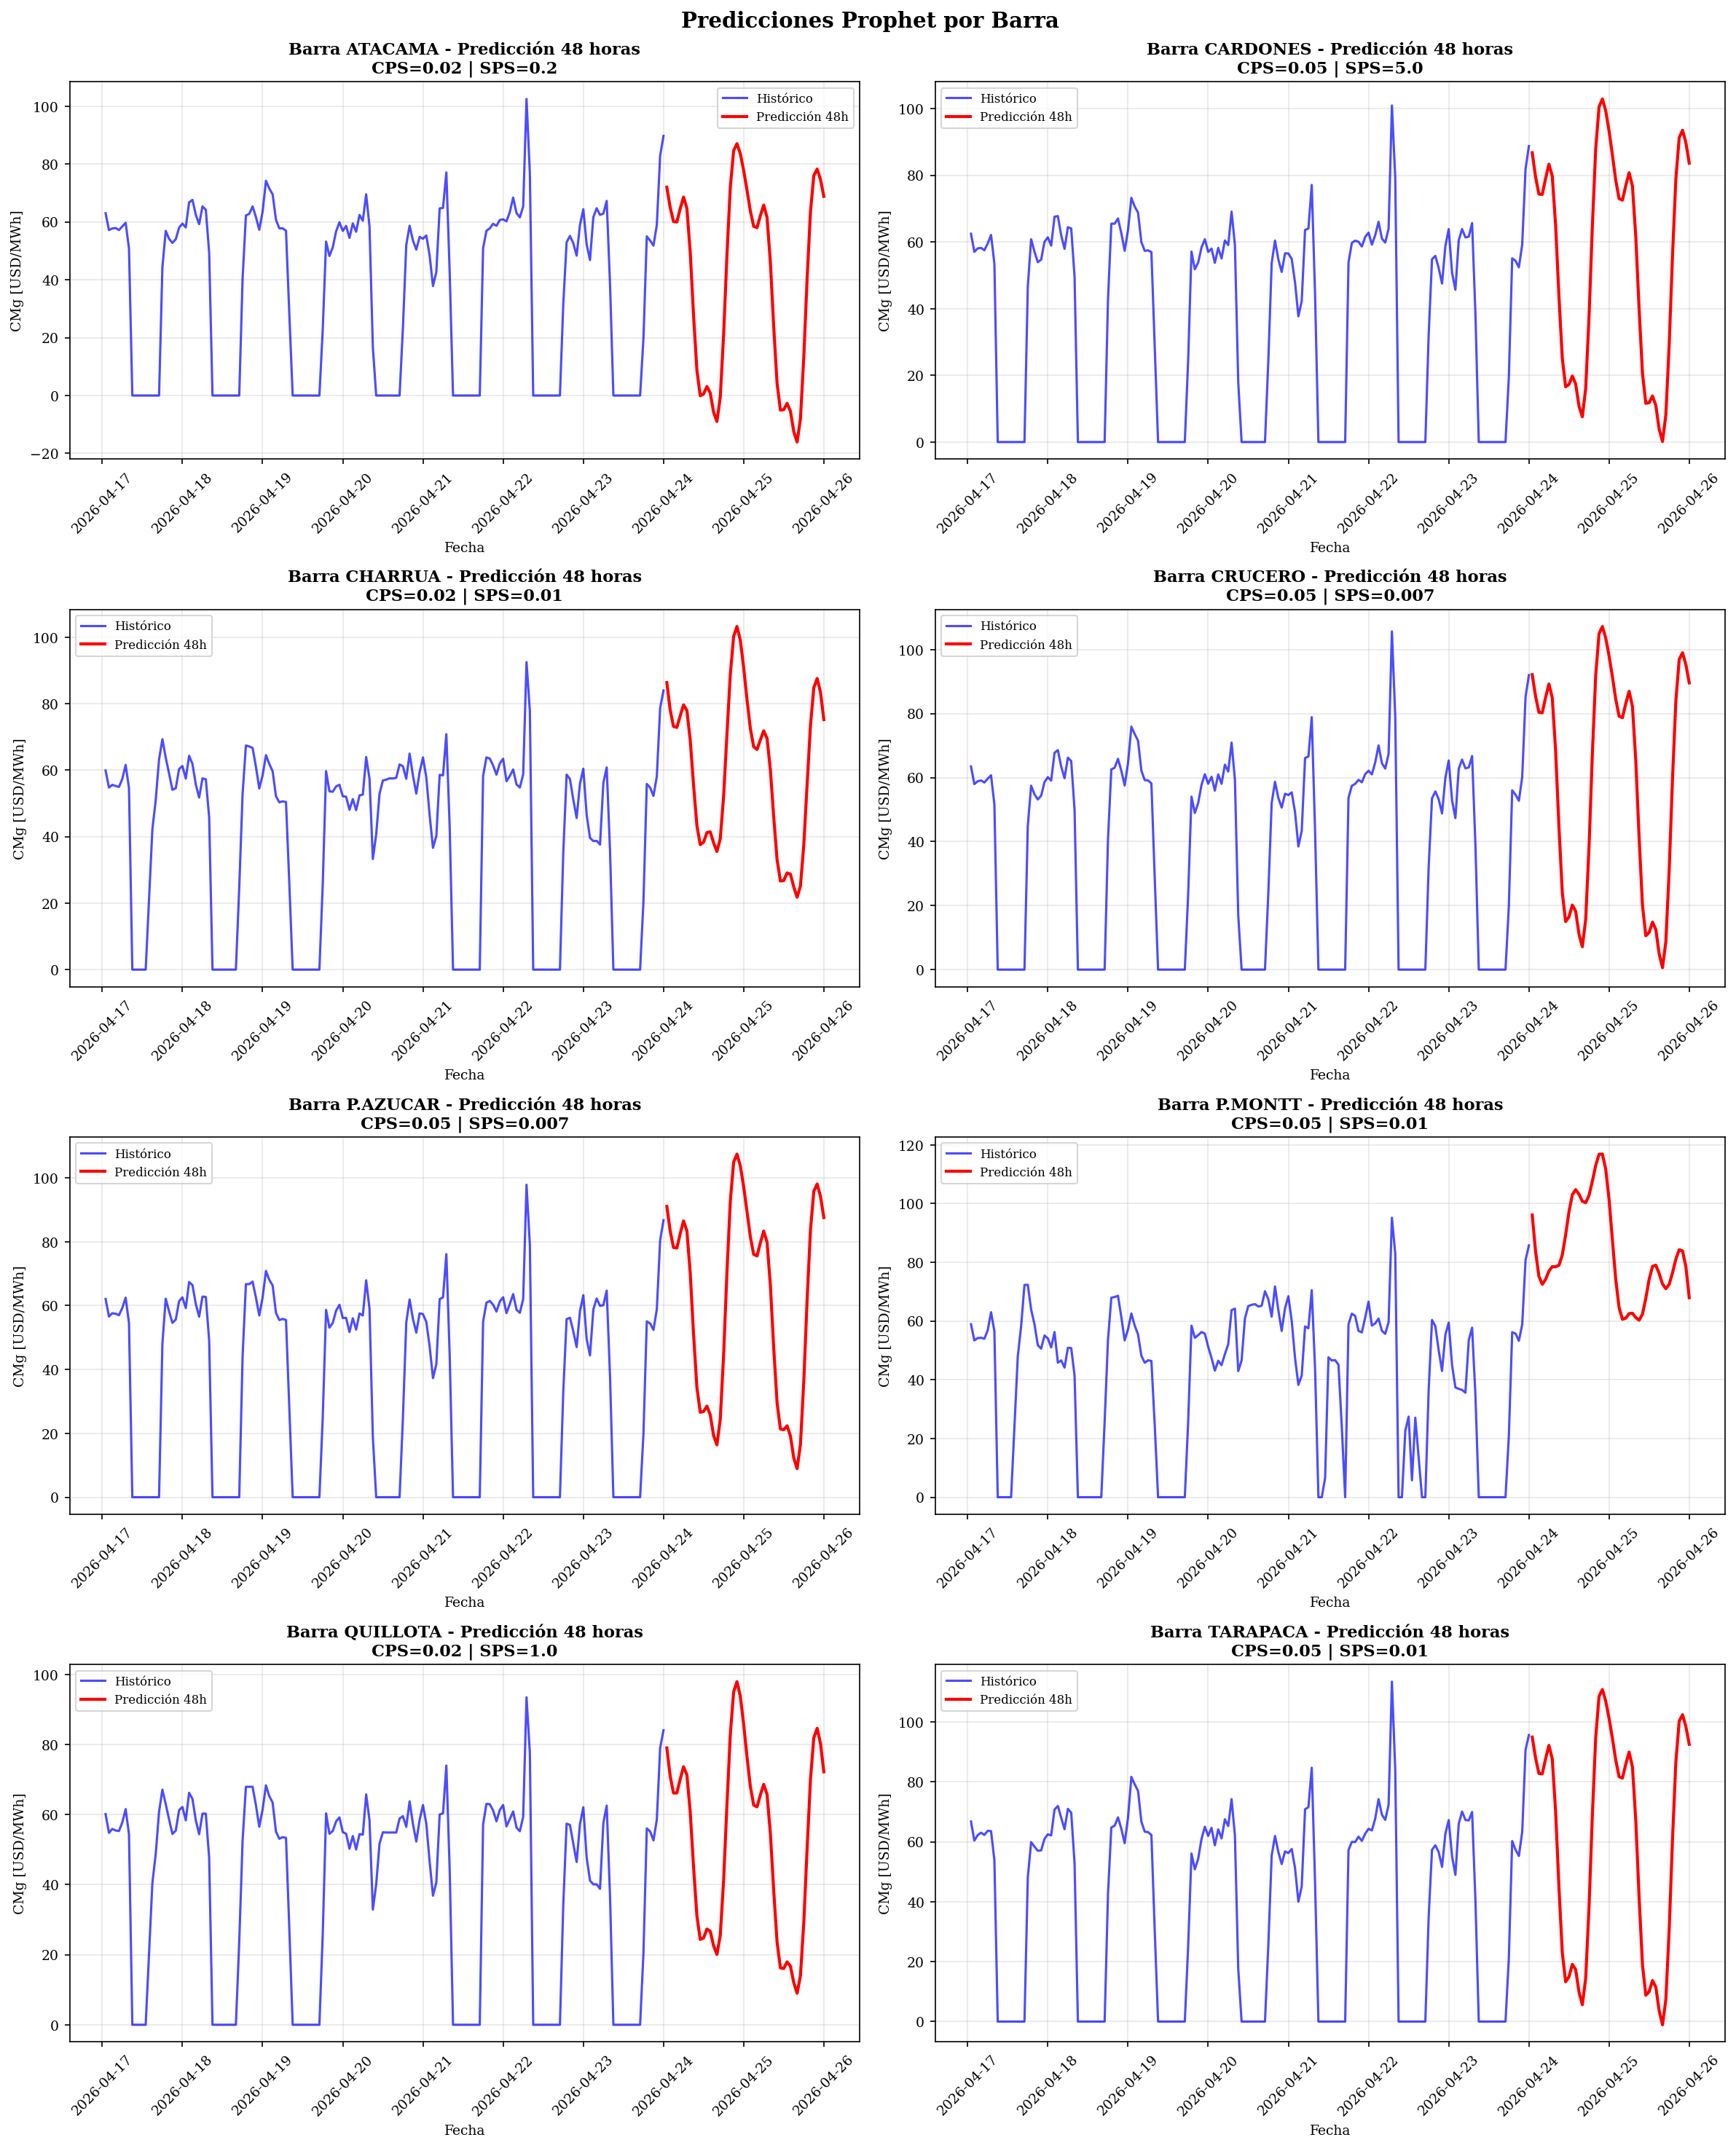
\includegraphics[width=0.95\textwidth]{imagenes/Posibles img/Predicciones por Barra.png}
    \caption{Predicciones de Prophet a 48 horas para las ocho barras del SEN, mostrando el histórico reciente (azul) y la proyección (rojo). Se aprecia el ciclo diario capturado por el modelo, con la caída característica durante el bloque solar y el alza en horas nocturnas.}
    \label{fig:prophet_pred48}
\end{figure}

Las predicciones a 48 horas confirman que Prophet captura correctamente la estructura del ciclo diario, reproduciendo la caída característica durante el bloque solar y el alza en horas de menor generación renovable. Sin embargo, se observa que en algunas barras la predicción alcanza valores negativos, lo que constituye una limitación física del modelo: el costo marginal no puede ser negativo en el SEN, pero Prophet, al ser un modelo de descomposición aditiva sin restricciones de dominio, puede extrapolar fuera del rango físicamente válido cuando la componente estacional supera a la tendencia. Esta limitación es inherente a la formulación de Prophet y refuerza la necesidad del TFT como componente complementario, cuya arquitectura de red neuronal le permite aprender implícitamente los límites del rango observado. Las predicciones de Prophet reportadas en el Capítulo 4 se truncan en 0 USD/MWh para evitar que esta limitación degrade artificialmente sus métricas de evaluación (Sección \ref{sec:modelo_prophet}); el residuo que consume $\text{TFT}_\text{LN}$ en la rama P+C, en cambio, se calcula sobre la predicción sin truncar, dado que truncarlo exigiría reentrenar el modelo de residuos sobre el nuevo objetivo.

\section{Temporal Fusion Transformer}

\subsection{Construcción de features y dataloaders}

El TFT recibe los datos estandarizados, según la transformación descrita en la Sección 3.2, junto con un conjunto de features organizadas en tres grupos según la taxonomía del TFT descrita en la Sección 2.3.4: covariables estáticas, covariables temporales conocidas (\texttt{known\_reals}) y covariables temporales desconocidas (\texttt{unknown\_reals}).

Se comparan dos estrategias de construcción de \texttt{known\_reals}, que constituyen las dos ramas metodológicas centrales evaluadas en este trabajo:

\begin{itemize}
    \item \textbf{Prophet + Clima (P+C):} las \texttt{known\_reals} corresponden a las cuatro componentes descompuestas por Prophet, tendencia (\texttt{trend}), estacionalidad anual (\texttt{yearly}), semanal (\texttt{weekly}) y diaria (\texttt{daily}), más un indicador binario de feriado nacional (\texttt{is\_holiday}). Es la estrategia originalmente adoptada en el diseño del modelo híbrido, dado que motiva directamente el esquema de ensamblaje Prophet-TFT descrito en la Sección 3.5.
    \item \textbf{Sol + Clima (S+C):} las \texttt{known\_reals} se reemplazan por tres variables de posición solar calculadas directamente mediante la librería \texttt{pvlib}: un indicador binario de horario de verano (\texttt{es\_horario\_verano}), el ángulo de elevación solar (\texttt{elevacion\_solar}) y su coseno (\texttt{cos\_elevacion}). El ángulo de elevación se obtiene mediante la función \texttt{get\_solarposition} del módulo \texttt{solarposition} de \texttt{pvlib}, aplicada sobre la marca temporal en UTC, calculada a partir de la hora local chilena considerando explícitamente los cambios de huso horario de verano/invierno, que en Chile no siguen una regla fija de calendario sino fechas específicas determinadas por decreto cada año; las coordenadas geográficas usadas para cada barra se detallan más adelante en esta subsección, junto con las variables climáticas.
\end{itemize}

La motivación de la rama S+C es evitar la dependencia de un modelo de descomposición intermedio para representar el ciclo diario y anual del costo marginal: la elevación solar es una variable física directamente observable que captura ambos ciclos de forma más directa que las componentes estimadas por Prophet, sin requerir un proceso de ajuste propio ni estar sujeta a los supuestos de la descomposición aditiva. Ambas ramas se evalúan de forma independiente (Prophet cuando corresponde, TFT de precios y de residuos, Stacking Optimization, TFT con DyT y Conformal Prediction) y se comparan empíricamente en el Capítulo 4.

Las \textit{covariables estáticas} incluyen, en ambas ramas, el identificador de barra (\texttt{serie\_id}), que permite al modelo aprender dinámicas temporales distintas para cada nodo del sistema sin necesidad de entrenar instancias separadas, tal como se describió en la Sección 2.3.4.

Las \textit{covariables temporales desconocidas} (\texttt{unknown\_reals}) son las mismas en ambas ramas. Para el TFT de precios corresponden a la serie estandarizada (\texttt{y\_real}) más las cinco variables climáticas horarias. Para el TFT de residuos, utilizado únicamente en la rama P+C dado que la rama S+C no calcula residuos de Prophet, corresponden al residuo estandarizado (\texttt{residuo}) más las mismas cinco variables climáticas. Deliberadamente no se incluyen lags manuales (por ejemplo, de 1, 24 o 168 horas) ni estadísticos móviles (medias o desviaciones estándar sobre ventanas de 24 o 168 horas): estas dependencias de corto y largo plazo se delegan íntegramente al mecanismo de atención y a las capas LSTM del encoder de 168 horas descrito a continuación, evitando representar explícitamente una estructura temporal que el modelo ya captura internamente.

Las variables climáticas corresponden a temperatura a 2 metros (\texttt{temperatura}), humedad relativa (\texttt{humedad}), velocidad del viento a 10 metros (\texttt{velocidad\_viento}), precipitación (\texttt{precipitacion}) y nubosidad (\texttt{nubosidad}), obtenidas con resolución horaria desde la API de archivo de Open-Meteo (\texttt{archive-api.open-meteo.com}), que provee datos de reanálisis ERA5 del Centro Europeo de Predicción Meteorológica a Medio Plazo (ECMWF). Los datos se obtienen para las coordenadas geográficas de la ciudad más representativa de cada barra: Iquique para Tarapacá, Antofagasta para Crucero, Copiapó para Cardones, Vallenar para Atacama, La Serena para Pan de Azúcar, Valparaíso para Quillota, Concepción para Charrúa y Puerto Montt para la barra homónima.

Cabe declarar una limitación de viabilidad operacional de esta fuente de datos, independiente de la validez causal del esquema \texttt{unknown\_reals}: ERA5 es un producto de reanálisis, no una observación en tiempo real, y se publica con un rezago del orden de días respecto de la fecha a la que corresponde. Esto significa que, aunque el modelo nunca recibe clima de horas futuras a la que predice --las cinco variables entran como \texttt{unknown\_reals}, solo disponibles para el encoder, nunca para el paso del decoder-- ni siquiera el clima de las horas más recientes de la propia ventana de encoder estaría disponible en operación real al momento de generar una predicción, porque ERA5 para esos días recientes todavía no ha sido publicado. El pipeline evaluado en este trabajo es, por lo tanto, causalmente correcto pero no directamente desplegable tal cual: una implementación operacional requeriría sustituir ERA5 por un producto de pronóstico meteorológico a corto plazo (por ejemplo, GFS o el pronóstico operacional de ECMWF) para las horas más recientes de la ventana de encoder, cuyo error de pronóstico degradaría en algún grado el desempeño reportado en el Capítulo 4. Evaluar esa degradación queda fuera del alcance de este trabajo.

La ventana de contexto se fija en $L = 168$ horas, equivalente a una semana completa, lo que permite al TFT acceder a un ciclo semanal completo de historia al realizar cada predicción. El horizonte de predicción es $h = 1$ hora, consistente con el objetivo de forecasting definido en la Sección 2.1.4. Para cada instante de predicción, el encoder mínimo se fija en $L/2 = 84$ horas para garantizar que todas las ventanas de entrenamiento tengan contexto suficiente. PyTorch Forecasting agrega automáticamente el índice de tiempo relativo (\texttt{add\_relative\_time\_idx}) y las escalas del target (\texttt{add\_target\_scales}) como features adicionales. Una ventana de contexto de dos semanas ($L = 336$ horas) y de 10 días ($L = 240$ horas) fue evaluada preliminarmente: el entrenamiento no fallaba de inmediato, pero colapsaba por falta de memoria hacia las épocas 10--15, y si bien hubiese sido posible reanudar el entrenamiento desde el último checkpoint guardado, el tiempo adicional requerido para completar las 100 épocas de esta forma no era viable dentro del presupuesto computacional del trabajo. Por lo tanto, $L = 168$ horas constituye el máximo viable bajo las restricciones computacionales del trabajo.

Los dataloaders se construyen de manera que el conjunto de validación incluye el período de entrenamiento más el de validación, y el conjunto de prueba incluye los tres períodos concatenados, preservando la continuidad del índice temporal (\texttt{time\_idx}) en todo momento. Se verifica explícitamente que el índice sea monótonamente creciente en cada conjunto para garantizar la causalidad temporal.

\subsection{Arquitectura y entrenamiento}

Los hiperparámetros del TFT se presentan en la Tabla \ref{tab:tft_config}. En la rama P+C se entrenan dos instancias del TFT con la misma configuración: una sobre la serie estandarizada de precios ($\text{TFT}_\text{LN}$ precios) y otra sobre los residuos de Prophet ($\text{TFT}_\text{LN}$ residuos); en la rama S+C se entrena únicamente la instancia de precios, dado que no existe un residuo de Prophet que modelar.

\begin{table}[htbp]
    \centering
    \begin{tabular}{ll}
        \toprule
        Hiperparámetro & Valor \\
        \midrule
        Learning rate inicial         & 0.001 \\
        Hidden size                   & 32 \\
        Attention heads               & 4 \\
        Dropout                       & 0.2 \\
        Hidden continuous size        & 8 \\
        Función de pérdida            & MAE \\
        Épocas máximas                & 100 \\
        Early stopping patience       & 15 épocas \\
        Reduce LR on plateau patience & 5 épocas \\
        Gradient clipping             & 0.1 \\
        Ventana de contexto $L$       & 168 horas \\
        Horizonte $h$                 & 1 hora \\
        \bottomrule
    \end{tabular}
    \caption{Hiperparámetros del TFT con LayerNorm.}
    \label{tab:tft_config}
\end{table}

A diferencia de la pérdida cuantílica general del TFT (Sección 2.3.4.7), en este trabajo el modelo se entrena minimizando directamente el MAE de la predicción puntual, lo que permite aplicar \textit{early stopping} sobre la misma métrica objetivo del problema; la cuantificación de incertidumbre se aborda por separado mediante Conformal Prediction (Sección 3.7), no mediante salidas cuantílicas del TFT.

El modelo se optimiza mediante Adam con tasa de aprendizaje inicial de 0.001, reducida automáticamente por un factor cuando la pérdida de validación no mejora durante 5 épocas consecutivas (\texttt{ReduceLROnPlateau}). El entrenamiento se detiene anticipadamente si la pérdida de validación no mejora en más de $10^{-4}$ durante 15 épocas consecutivas. El gradiente se recorta a 0.1 para estabilizar el entrenamiento en presencia de los spikes del costo marginal. El tiempo de entrenamiento de cada modelo por barra es de aproximadamente 12 horas en un PC de trabajo y aproximadamente 3:30 horas en el cluster del NLHPC.

Esta restricción de cómputo --entrenar un único TFT ya toma horas, frente a segundos por combinación de hiperparámetros en Prophet-- es la razón por la que los hiperparámetros del TFT (Tabla \ref{tab:tft_config}) se fijan de antemano en vez de buscarse por barra, a diferencia de Prophet, cuyo \texttt{changepoint\_prior\_scale} y \texttt{seasonality\_prior\_scale} sí se optimizan mediante una grilla específica para cada una de las ocho barras (Tabla \ref{tab:prophet_params}). Esto constituye una limitación explícita, no solo un dato operativo: introduce un esfuerzo de ajuste asimétrico entre ambos modelos, que afecta potencialmente a dos comparaciones distintas de este trabajo. Primero, a la comparación entre S+C (o P+C) y Prophet solo (Sección \ref{sec:modelo_prophet}): un TFT con hiperparámetros optimizados por barra podría, en principio, ampliar aún más su ventaja sobre Prophet, o reducirla si los valores fijos usados ya están cerca del óptimo; este trabajo no puede distinguir entre ambos escenarios. Segundo, y de forma más directa, a la comparación entre $\text{TFT}_\text{LN}$ y $\text{TFT}_\text{DyT}$ (Sección \ref{sec:ln_vs_dyt}): ambas arquitecturas se evalúan bajo la misma configuración de hiperparámetros, que no fue optimizada específicamente para ninguna de las dos, por lo que la ventaja sistemática mostrada por LayerNorm podría no sostenerse, o podría ampliarse, bajo una búsqueda de hiperparámetros independiente para cada arquitectura.

El TFT se entrena, en el resto de este trabajo, sin fijar una semilla aleatoria para el generador de números de PyTorch, de modo que la comparación entre $\text{TFT}_\text{LN}$ y $\text{TFT}_\text{DyT}$ (Sección \ref{sec:ln_vs_dyt}) podría, en principio, reflejar variabilidad de inicialización más que una diferencia sistemática entre arquitecturas. Para acotar esta posibilidad, se repite el entrenamiento de S+C con 5 semillas distintas (fijadas mediante \texttt{pl.seed\_everything}, no utilizado en el resto del pipeline) para tres barras piloto (Atacama, Charrúa, Puerto Montt) y ambas arquitecturas, manteniendo el resto de la configuración de la Tabla \ref{tab:tft_config} sin cambios, y se reporta la media y desviación estándar del MAE de prueba sobre las 5 réplicas (Sección \ref{sec:seeds_ln_dyt}).

\subsection{Curvas de aprendizaje}

La Figura \ref{fig:tft_learning_curves} presenta las curvas de aprendizaje para las ocho barras del SEN, mostrando la pérdida (MAE) en los conjuntos de entrenamiento y validación para ambos modelos.

\begin{figure}[htbp]
    \centering
    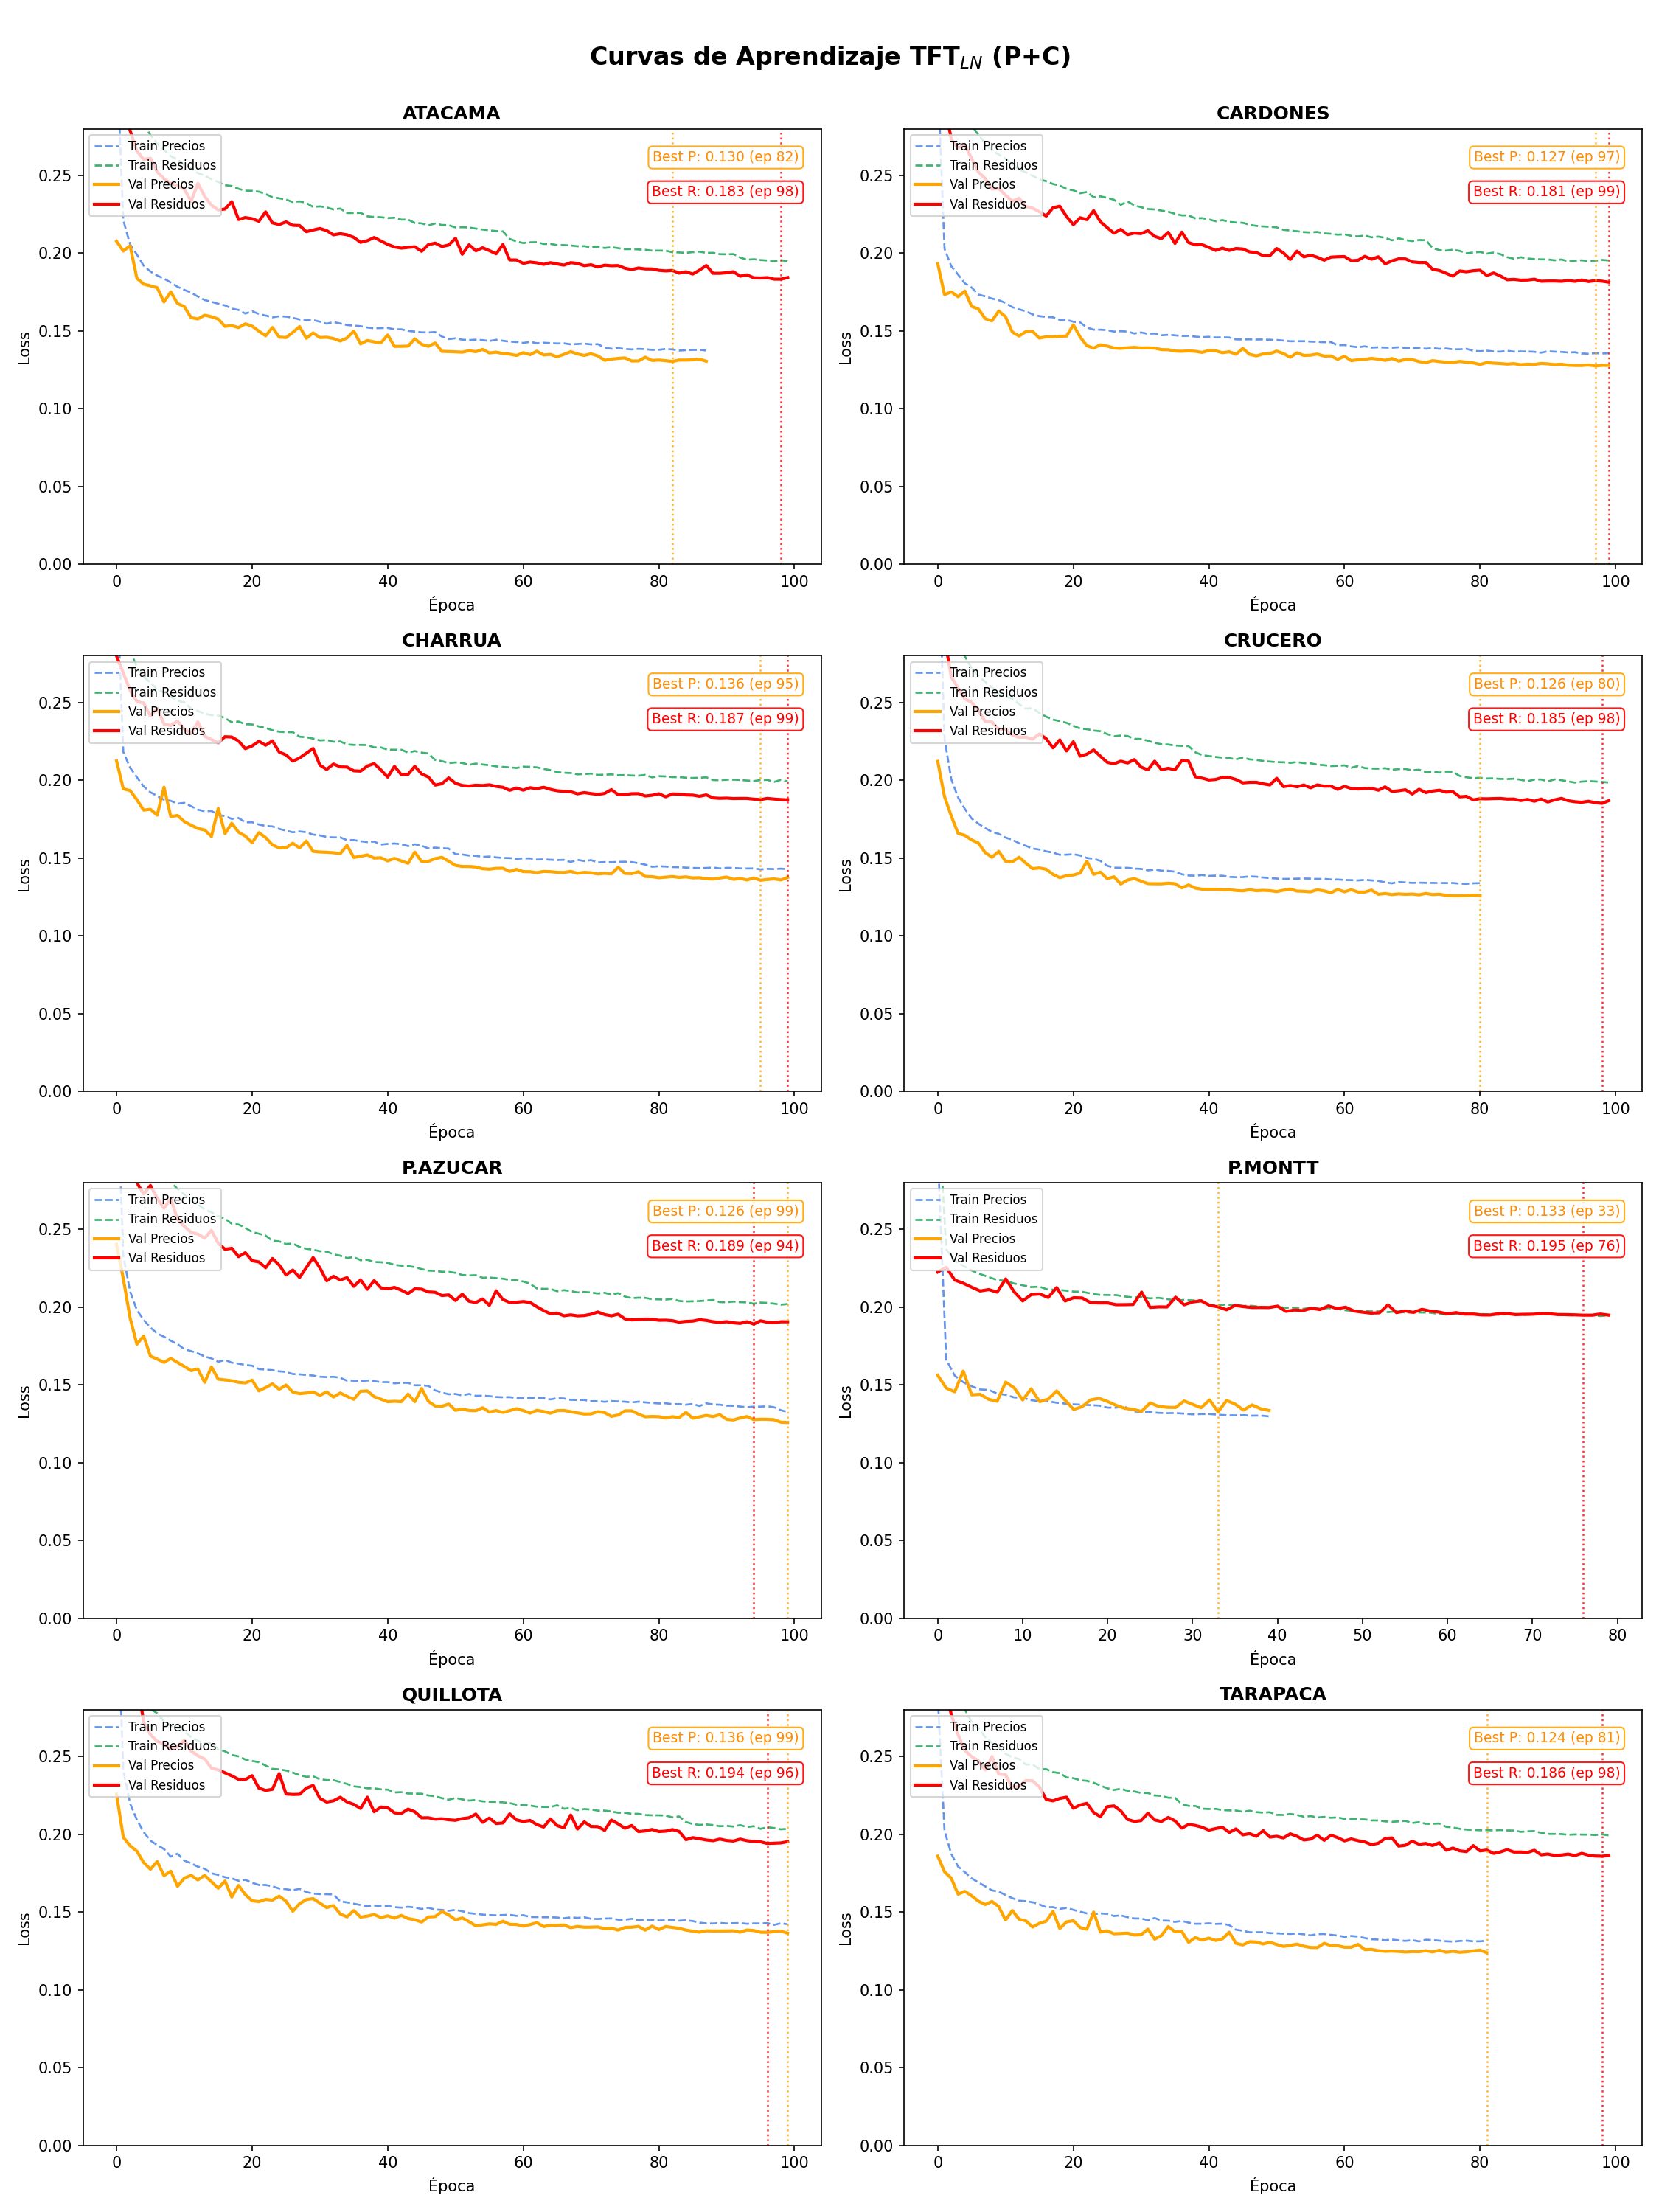
\includegraphics[width=0.95\textwidth]{imagenes/Posibles img/Curvas Aprendizaje LN.png}
    \caption{Curvas de aprendizaje del TFT con LayerNorm para las ocho barras del SEN. Se muestran la pérdida (MAE) de entrenamiento y validación para los modelos de precios y residuos. Las líneas verticales indican la época de mejor desempeño en validación.}
    \label{fig:tft_learning_curves}
\end{figure}

Las curvas muestran convergencia estable en la mayoría de las barras sin señales de sobreajuste severo. La pérdida de validación del modelo de precios converge en torno a 0.124--0.136, mientras que la del modelo de residuos se estabiliza alrededor de 0.181--0.195, lo que es esperable dado que los residuos de Prophet son intrínsecamente más difíciles de predecir que la serie original al haber eliminado la estructura sistemática de largo plazo. La mayoría de los modelos alcanza su mejor desempeño en épocas avanzadas del entrenamiento (entre las épocas 80 y 99), lo que indica que el límite de 100 épocas es adecuado y que el early stopping no se activa prematuramente; Puerto Montt es la excepción, con el modelo de precios deteniéndose de forma más temprana (mejor época 33), consistente con la mayor volatilidad estructural de esta barra ya documentada en la Sección 3.1.

\section{Stacking Optimization}

\subsection{Estrategias de ensamblaje}

El Stacking Optimization combina las predicciones de Prophet y las dos instancias del TFT mediante una combinación lineal convexa con pesos aprendidos sobre el conjunto de validación, siguiendo el marco descrito en la Sección 2.5. Se evalúan seis estrategias de ensamblaje que cubren desde los modelos base individuales hasta combinaciones progresivamente más complejas:

\begin{enumerate}
    \item \textbf{Prophet solo:} predicción directa de Prophet sin combinación.
    \item \textbf{$\text{TFT}_\text{LN}$ precios solo:} predicción directa del TFT entrenado sobre la serie de precios.
    \item \textbf{Prophet $+$ $\text{TFT}_\text{LN}$ precios:} combinación convexa $\hat{y} = w_1 \hat{y}^{\text{Prophet}} + w_2 \hat{y}^{\text{TFT}_\text{P}}$.
    \item \textbf{Prophet $+$ $\text{TFT}_\text{LN}$ residuos (D):} suma directa $\hat{y} = \hat{y}^{\text{Prophet}} + \hat{r}^{\text{TFT}_\text{R}}$ con pesos fijos $w_1 = w_2 = 1$.
    \item \textbf{Prophet $+$ $\text{TFT}_\text{LN}$ residuos (Opt):} combinación convexa $\hat{y} = w_1 \hat{y}^{\text{Prophet}} + w_2 \hat{r}^{\text{TFT}_\text{R}}$ con pesos optimizados.
    \item \textbf{(Prophet $+$ residuos) $+$ $\text{TFT}_\text{LN}$ precios (opt):} combinación convexa entre la predicción híbrida Prophet-residuos con suma directa y el $\text{TFT}_\text{LN}$ de precios, $\hat{y} = w_1 (\hat{y}^{\text{Prophet}} + \hat{r}^{\text{TFT}_\text{R}}) + w_2 \hat{y}^{\text{TFT}_\text{P}}$, con pesos optimizados.
\end{enumerate}

En todas las estrategias con optimización de pesos se impone la restricción de combinación convexa $w_1 + w_2 = 1$ con $w_1, w_2 \geq 0$, de modo que los pesos son interpretables como cuotas de participación de cada componente. Los pesos se estiman minimizando el MAE sobre el conjunto de validación y se aplican sin reestimación al conjunto de prueba.

\subsection{Métodos de optimización de pesos}

Para las estrategias que requieren optimización de pesos se comparan ocho métodos numéricos sobre el mismo problema de un grado de libertad ($w_1$, con $w_2 = 1 - w_1$): búsqueda en grilla con resoluciones de 21, 41 y 101 puntos (\textit{Grid\_21}, \textit{Grid\_41}, \textit{Grid\_101}), Nelder-Mead, SLSQP, L-BFGS-B, Evolución Diferencial y búsqueda aleatoria con 1.000 iteraciones (\textit{Random\_1000}), más Regresión Ridge ($\alpha = 0.01$) como comparación aparte: Ridge no optimiza la misma función objetivo MAE, sino que resuelve en forma cerrada un problema distinto (mínimos cuadrados con penalización $\ell_2$), por lo que se incluye para verificar que un estimador de uso común no se aleja del óptimo de los ocho anteriores, no como un noveno método sobre el mismo problema. Todos optimizan sobre el conjunto de validación y los pesos resultantes se evalúan en prueba sin reajuste.

Como se muestra en la Sección 4.3.1, la elección de método resulta irrelevante para la calidad del resultado final: al ser la función objetivo MAE convexa y unimodal en una variable, los ocho métodos numéricos convergen esencialmente al mismo mínimo, con diferencias inferiores al 0.1\%, y Ridge tampoco se aparta de ese óptimo de forma apreciable pese a resolver un problema distinto. La diferencia práctica entre métodos es el tiempo de cómputo, irrelevante a esta escala (SLSQP y Ridge bajo 0.05\,s en la mayoría de las barras; la búsqueda aleatoria, la más lenta, 0.5--1.2\,s); los resultados reportados en el resto de este trabajo emplean indistintamente el método con menor MAE de cada barra y estrategia.

\section{TFT con Dynamic Tanh}

El $\text{TFT}_\text{DyT}$ es una variante del TFT con LayerNorm descrito en la Sección 3.4 en la que todas las capas LayerNorm de la arquitectura son reemplazadas por capas Dynamic Tanh (DyT), siguiendo la sustitución uniforme descrita en la Sección 2.4.5. La configuración de features, dataloaders, hiperparámetros y protocolo de entrenamiento es idéntica a la del $\text{TFT}_\text{LN}$, con la única diferencia en el mecanismo de normalización. El parámetro $\alpha$ de cada capa DyT se inicializa en $\alpha_0 = 0.5$ con $\boldsymbol{\gamma} = \mathbf{1}$ y $\boldsymbol{\beta} = \mathbf{0}$, siguiendo la recomendación de Zhu et al. (2025) para modelos no-LLM descrita en la Sección 2.4.3. El mismo esquema de Stacking Optimization descrito en la Sección 3.5, con las seis estrategias de ensamblaje y los ocho métodos numéricos de optimización de pesos más Ridge, se aplica de forma idéntica sobre las predicciones del $\text{TFT}_\text{DyT}$, sustituyendo únicamente las predicciones puntuales de entrada por las del modelo con DyT.

\subsection{Curvas de aprendizaje}

La Figura \ref{fig:dyt_learning_curves} presenta las curvas de aprendizaje del $\text{TFT}_\text{DyT}$ para las ocho barras del SEN.

\begin{figure}[htbp]
    \centering
    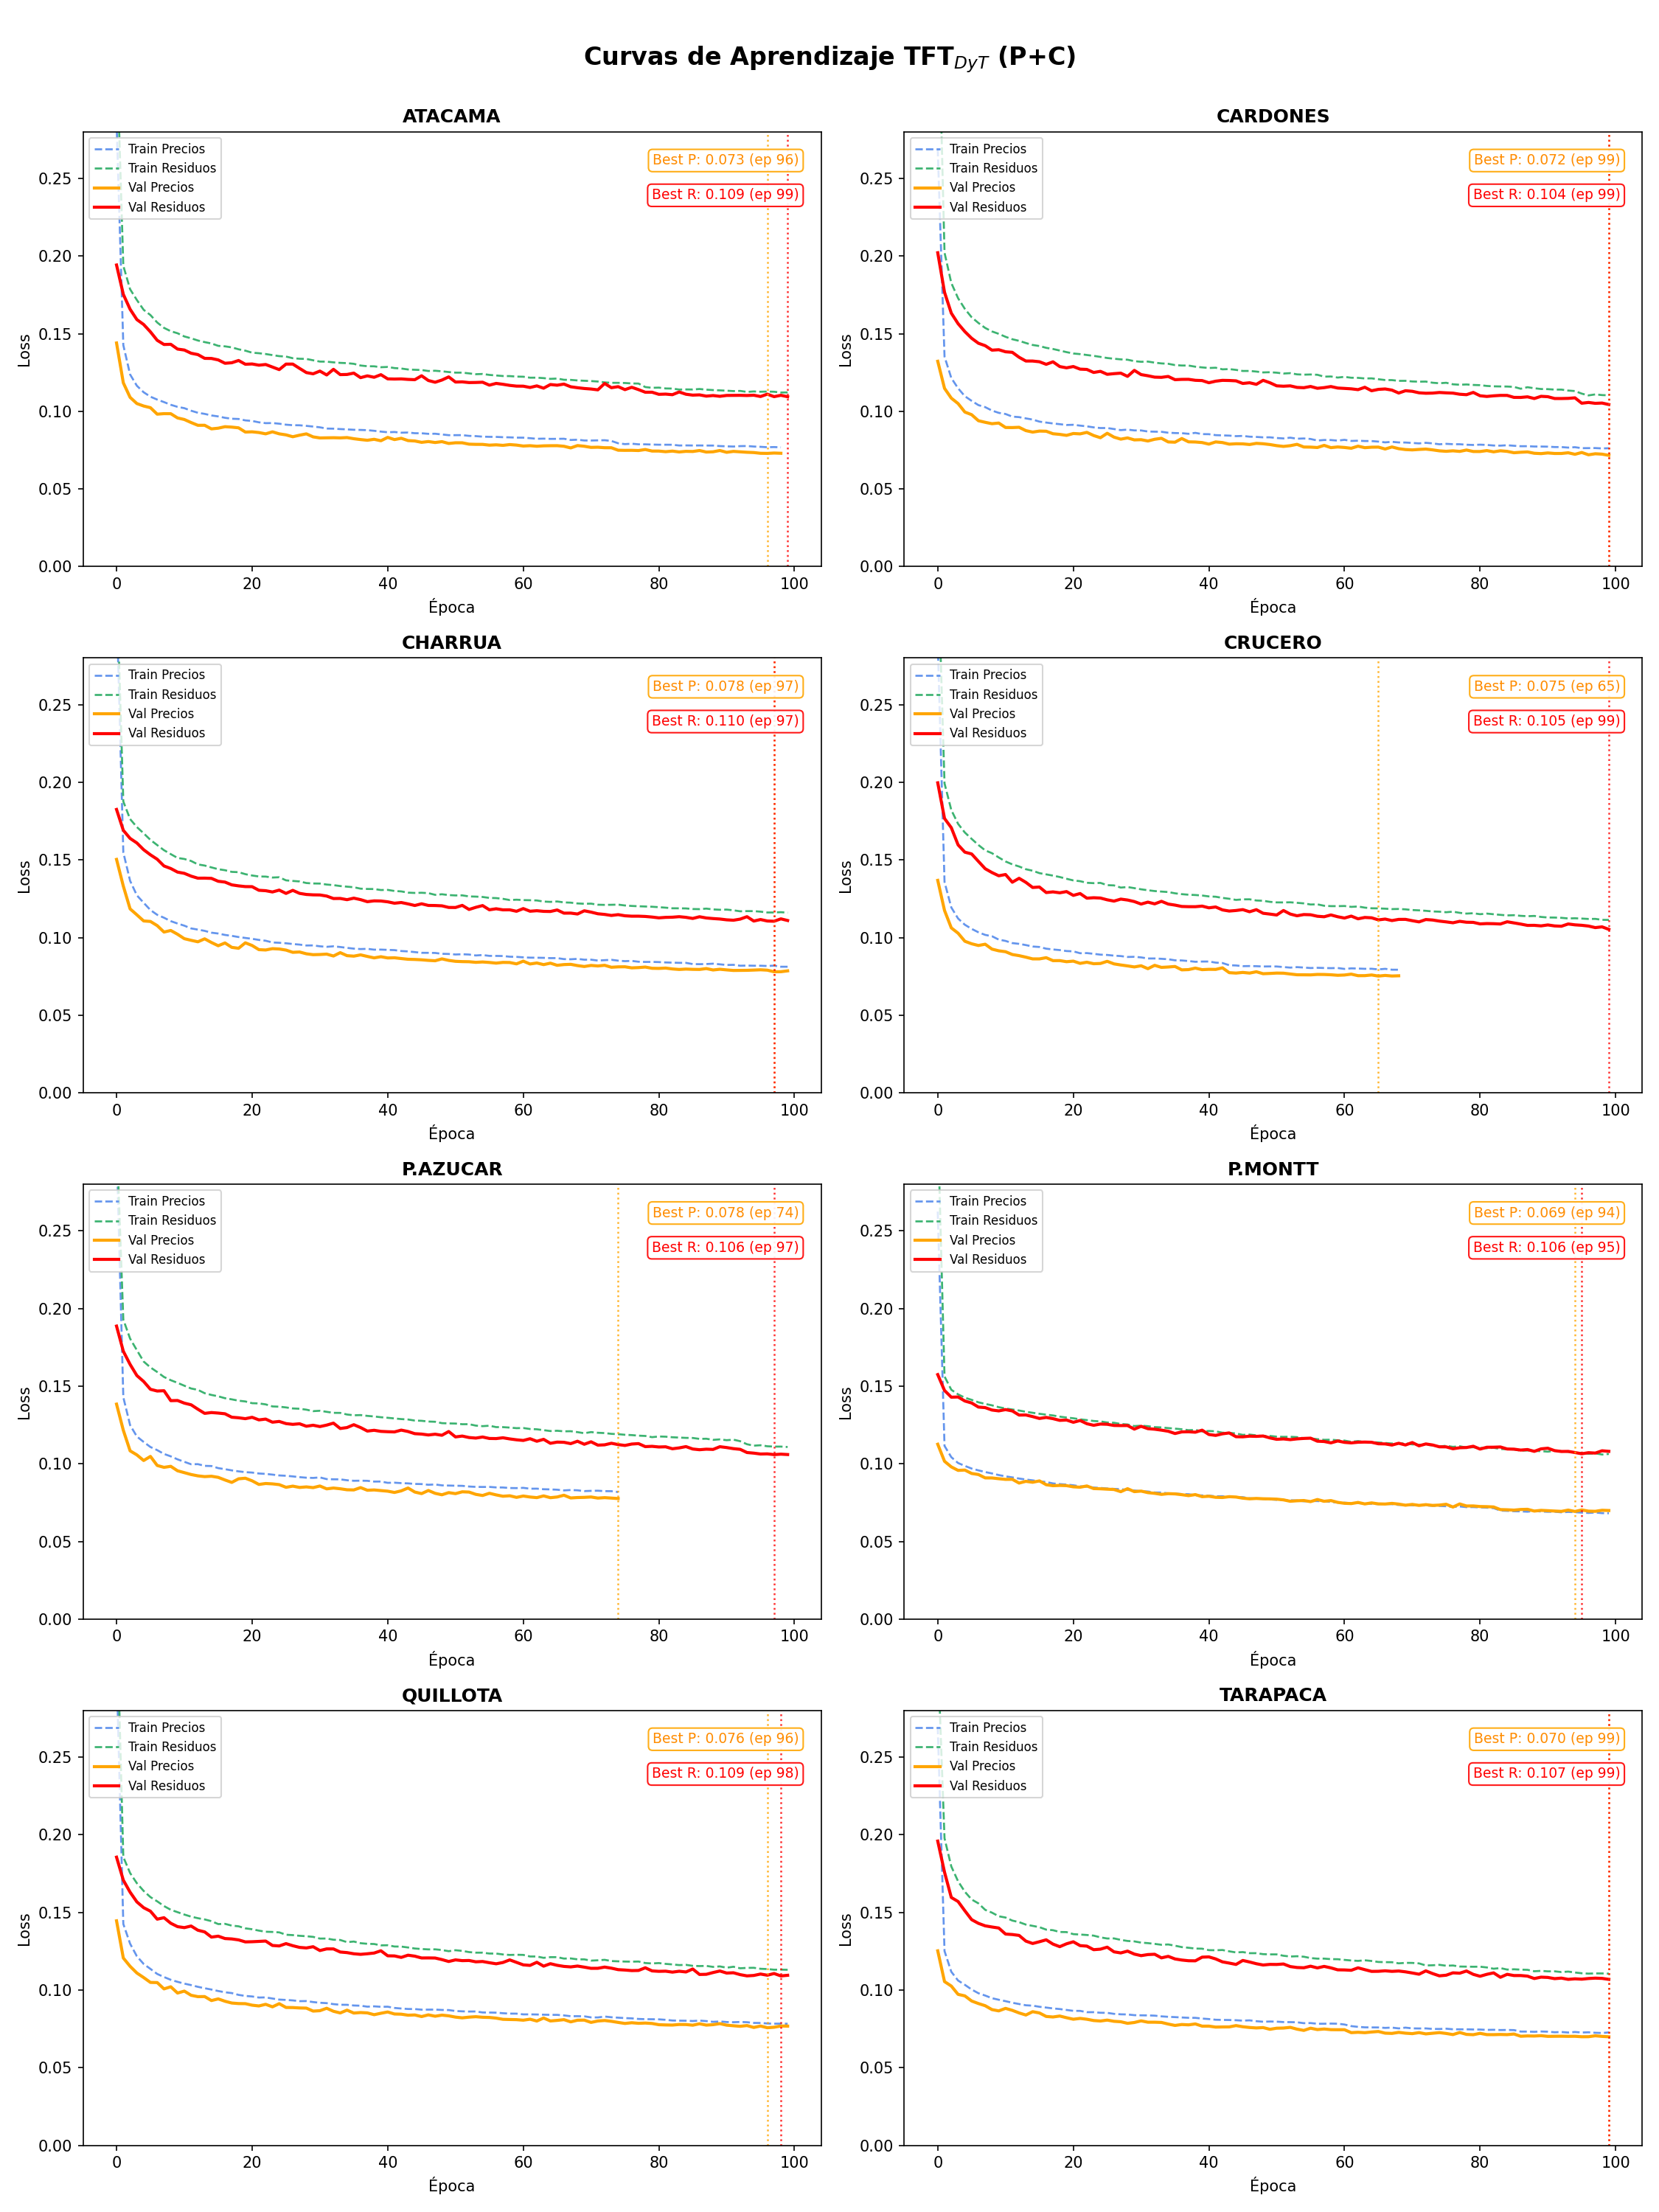
\includegraphics[width=0.95\textwidth]{imagenes/Posibles img/Curvas Aprendizaje DyT.png}
    \caption{Curvas de aprendizaje del TFT con DyT para las ocho barras del SEN. Se muestran la pérdida (MAE) de entrenamiento y validación para los modelos de precios y residuos. Las líneas verticales indican la época de mejor desempeño en validación.}
    \label{fig:dyt_learning_curves}
\end{figure}

Al igual que con $\text{TFT}_\text{LN}$, las curvas muestran una convergencia estable sin señales de sobreajuste severo: la pérdida de entrenamiento y de validación decrecen de forma conjunta y se estabilizan hacia el final del entrenamiento, sin la divergencia creciente entre ambas que caracterizaría al sobreajuste. La pérdida de validación del modelo de precios converge en torno a 0.069--0.078, y la del modelo de residuos alrededor de 0.104--0.110. La mayoría de los modelos alcanza su mejor desempeño en épocas avanzadas del entrenamiento, mayoritariamente entre las épocas 94 y 99, con algunas excepciones que se estabilizan algo antes (Crucero, precios, época 65).

\subsection{\texorpdfstring{Análisis del parámetro $\alpha$ aprendido}{Análisis del parámetro alfa aprendido}}

La Figura \ref{fig:alpha_dyt} presenta los valores del parámetro $\alpha$ aprendido por cada capa DyT del $\text{TFT}_\text{DyT}$, agrupados por módulo de la arquitectura. La línea roja punteada indica el valor de inicialización $\alpha_0 = 0.5$.

\begin{figure}[htbp]
    \centering
    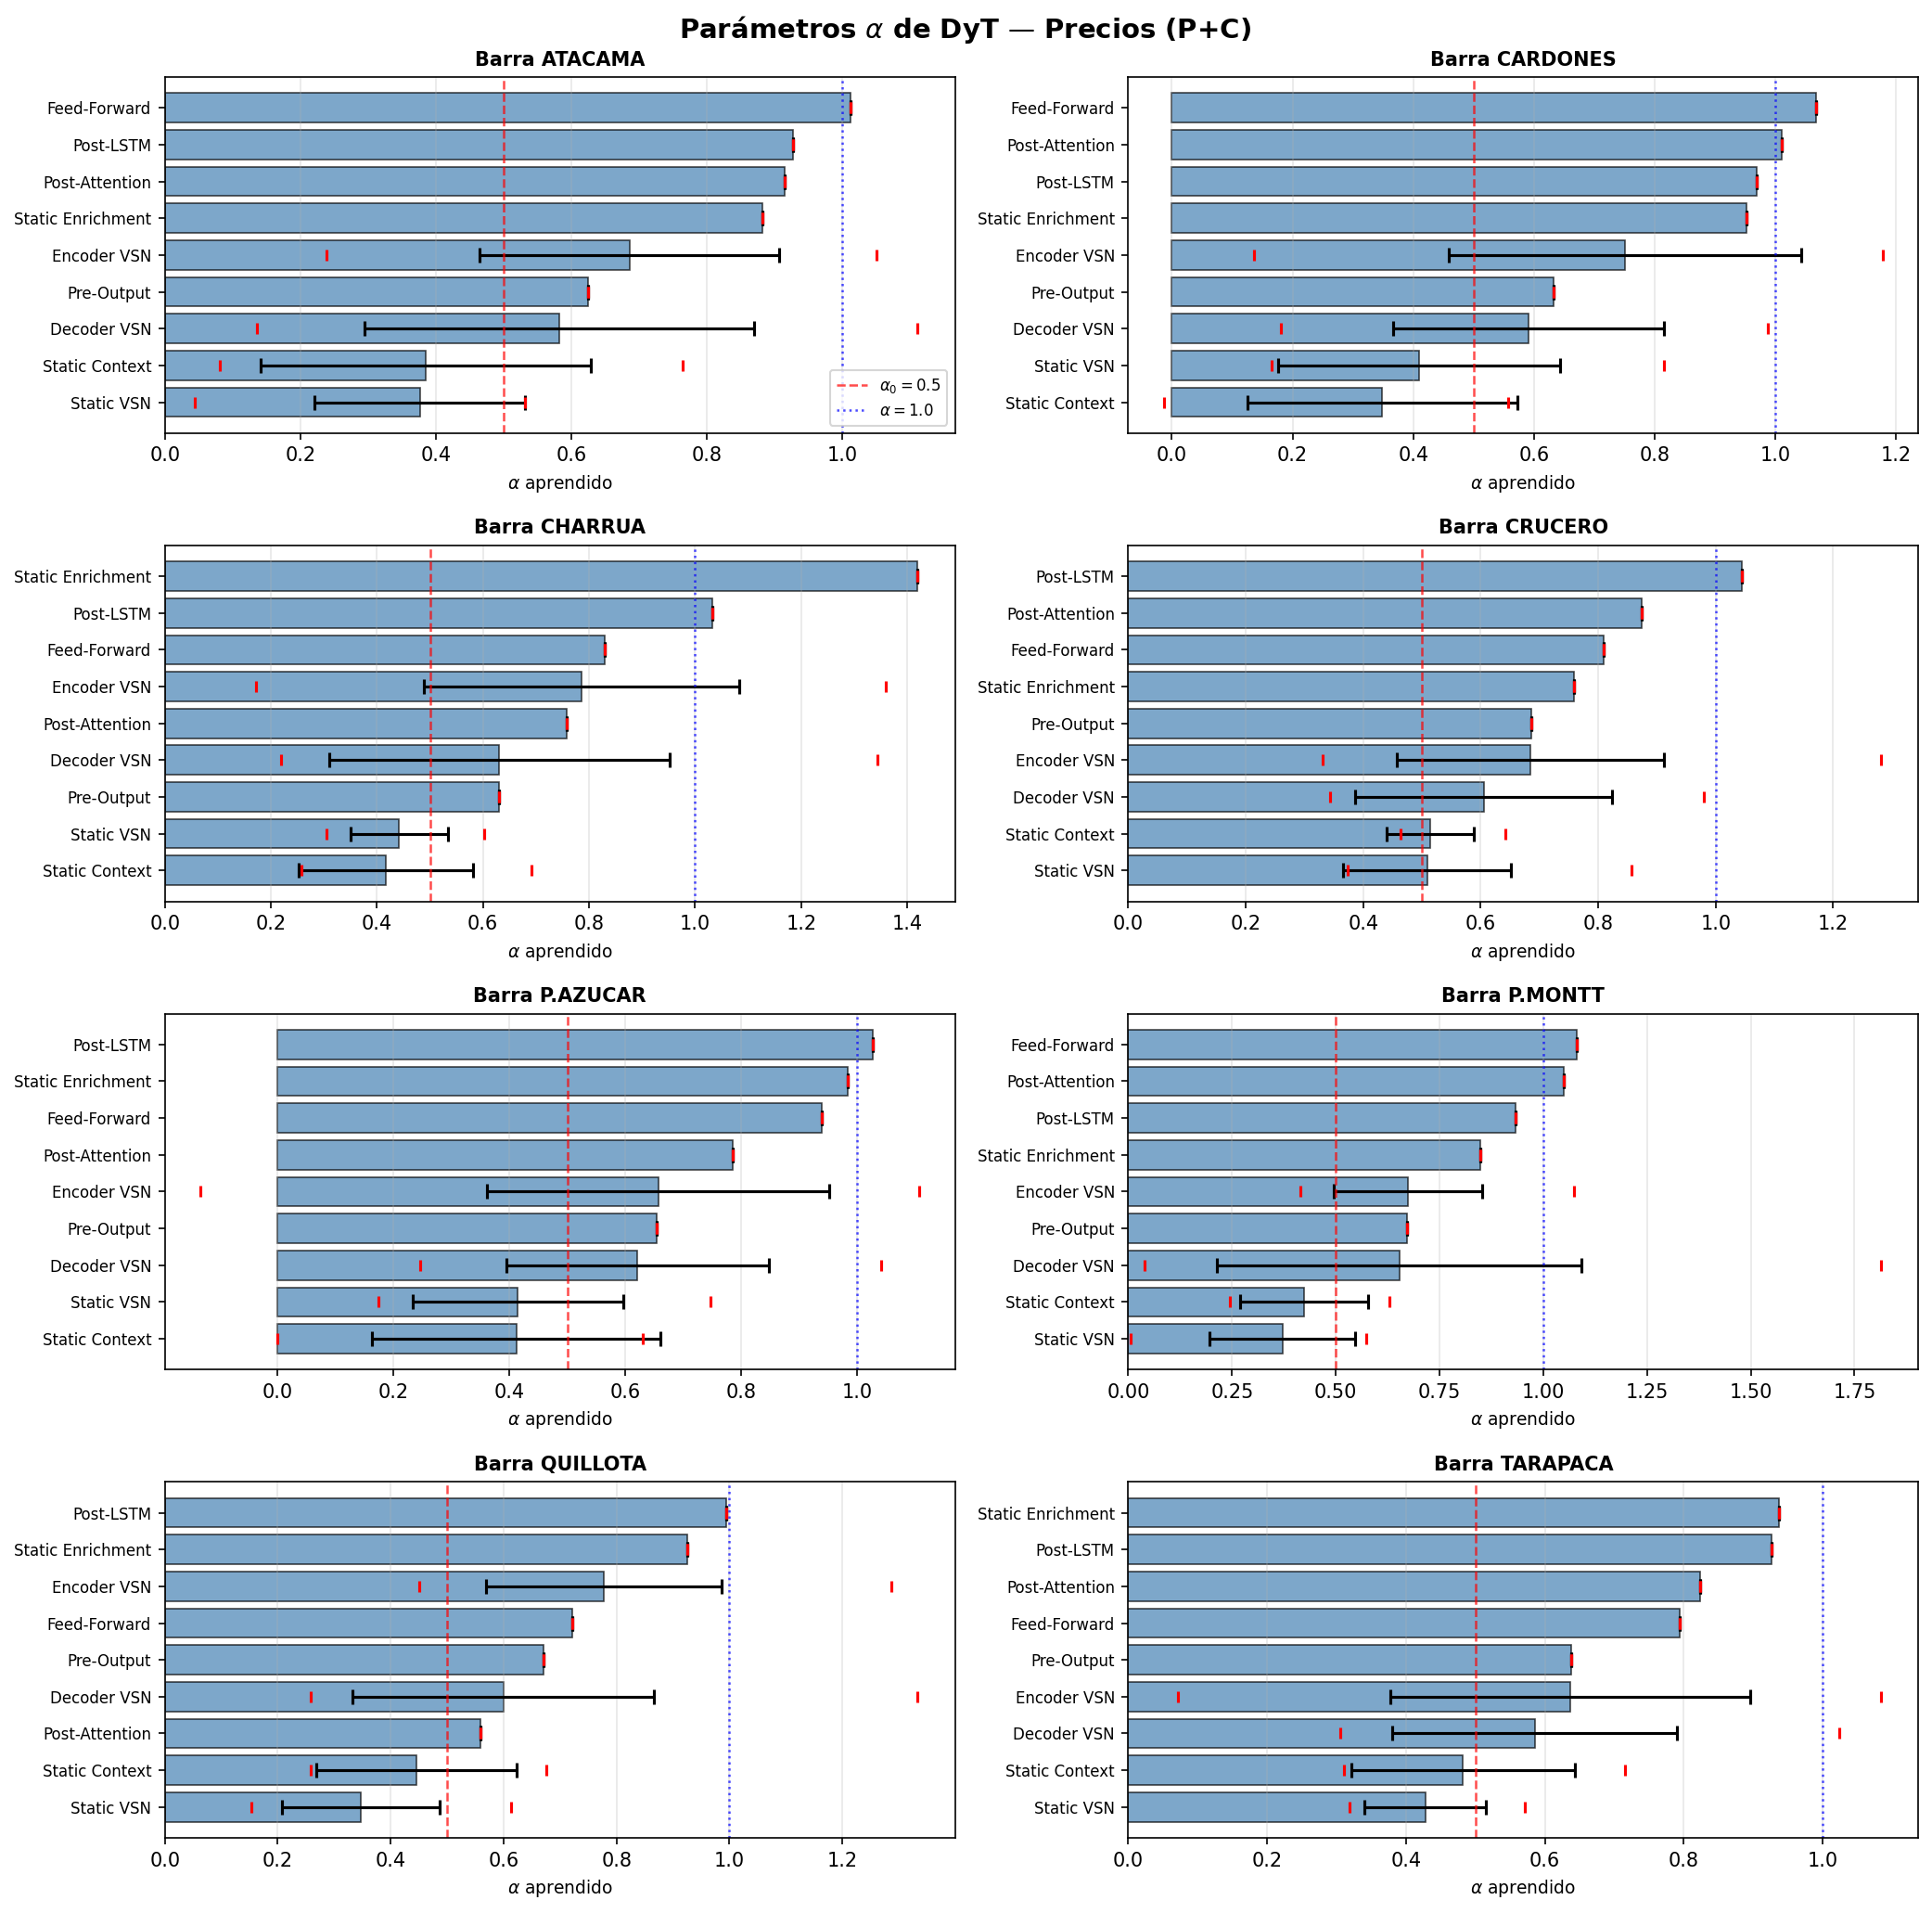
\includegraphics[width=0.85\textwidth]{imagenes/Posibles img/Alphas Aprendidos Precios.png}
    \caption{Valores del parámetro $\alpha$ aprendido por las capas DyT del $\text{TFT}_\text{DyT}$ para las ocho barras del SEN, agrupados por módulo de la arquitectura. Las barras muestran la media por módulo, las líneas de error la desviación estándar, y los marcadores rojos el mínimo y máximo. La línea roja punteada indica el valor de inicialización $\alpha_0 = 0.5$.}
    \label{fig:alpha_dyt}
\end{figure}

El resultado central de este análisis es que los valores de $\alpha$ se dispersaron significativamente desde el valor de inicialización $\alpha_0 = 0.5$, cubriendo un rango de $-0.13$ a $1.81$ al final del entrenamiento, con algunas capas individuales incluso aprendiendo valores levemente negativos lo que sigue siendo una transformación válida, dado que $\tanh$ es una función impar y un $\alpha$ negativo solo invierte la polaridad de esa unidad de squashing. Esto confirma que DyT efectivamente aprendió a normalizar de manera adaptativa durante el entrenamiento, en lugar de mantener una compresión fija, tal como predice la teoría de Zhu et al. (2025). Los módulos de selección de variables, Encoder VSN, Decoder VSN y Static VSN, presentan mayor dispersión entre capas que los módulos de más alto nivel como Feed-Forward y Post-LSTM, lo que refleja la heterogeneidad entre las features procesadas en cada módulo.

\subsection{Curvas de aprendizaje de S+C}

La Figura \ref{fig:sc_learning_curves} presenta las curvas de aprendizaje de la rama S+C para las ocho barras del SEN, comparando directamente $\text{TFT}_\text{LN}$ y $\text{TFT}_\text{DyT}$ sobre el único modelo que entrena esta rama, sin residuos de Prophet (Sección 3.4.1).

\begin{figure}[htbp]
    \centering
    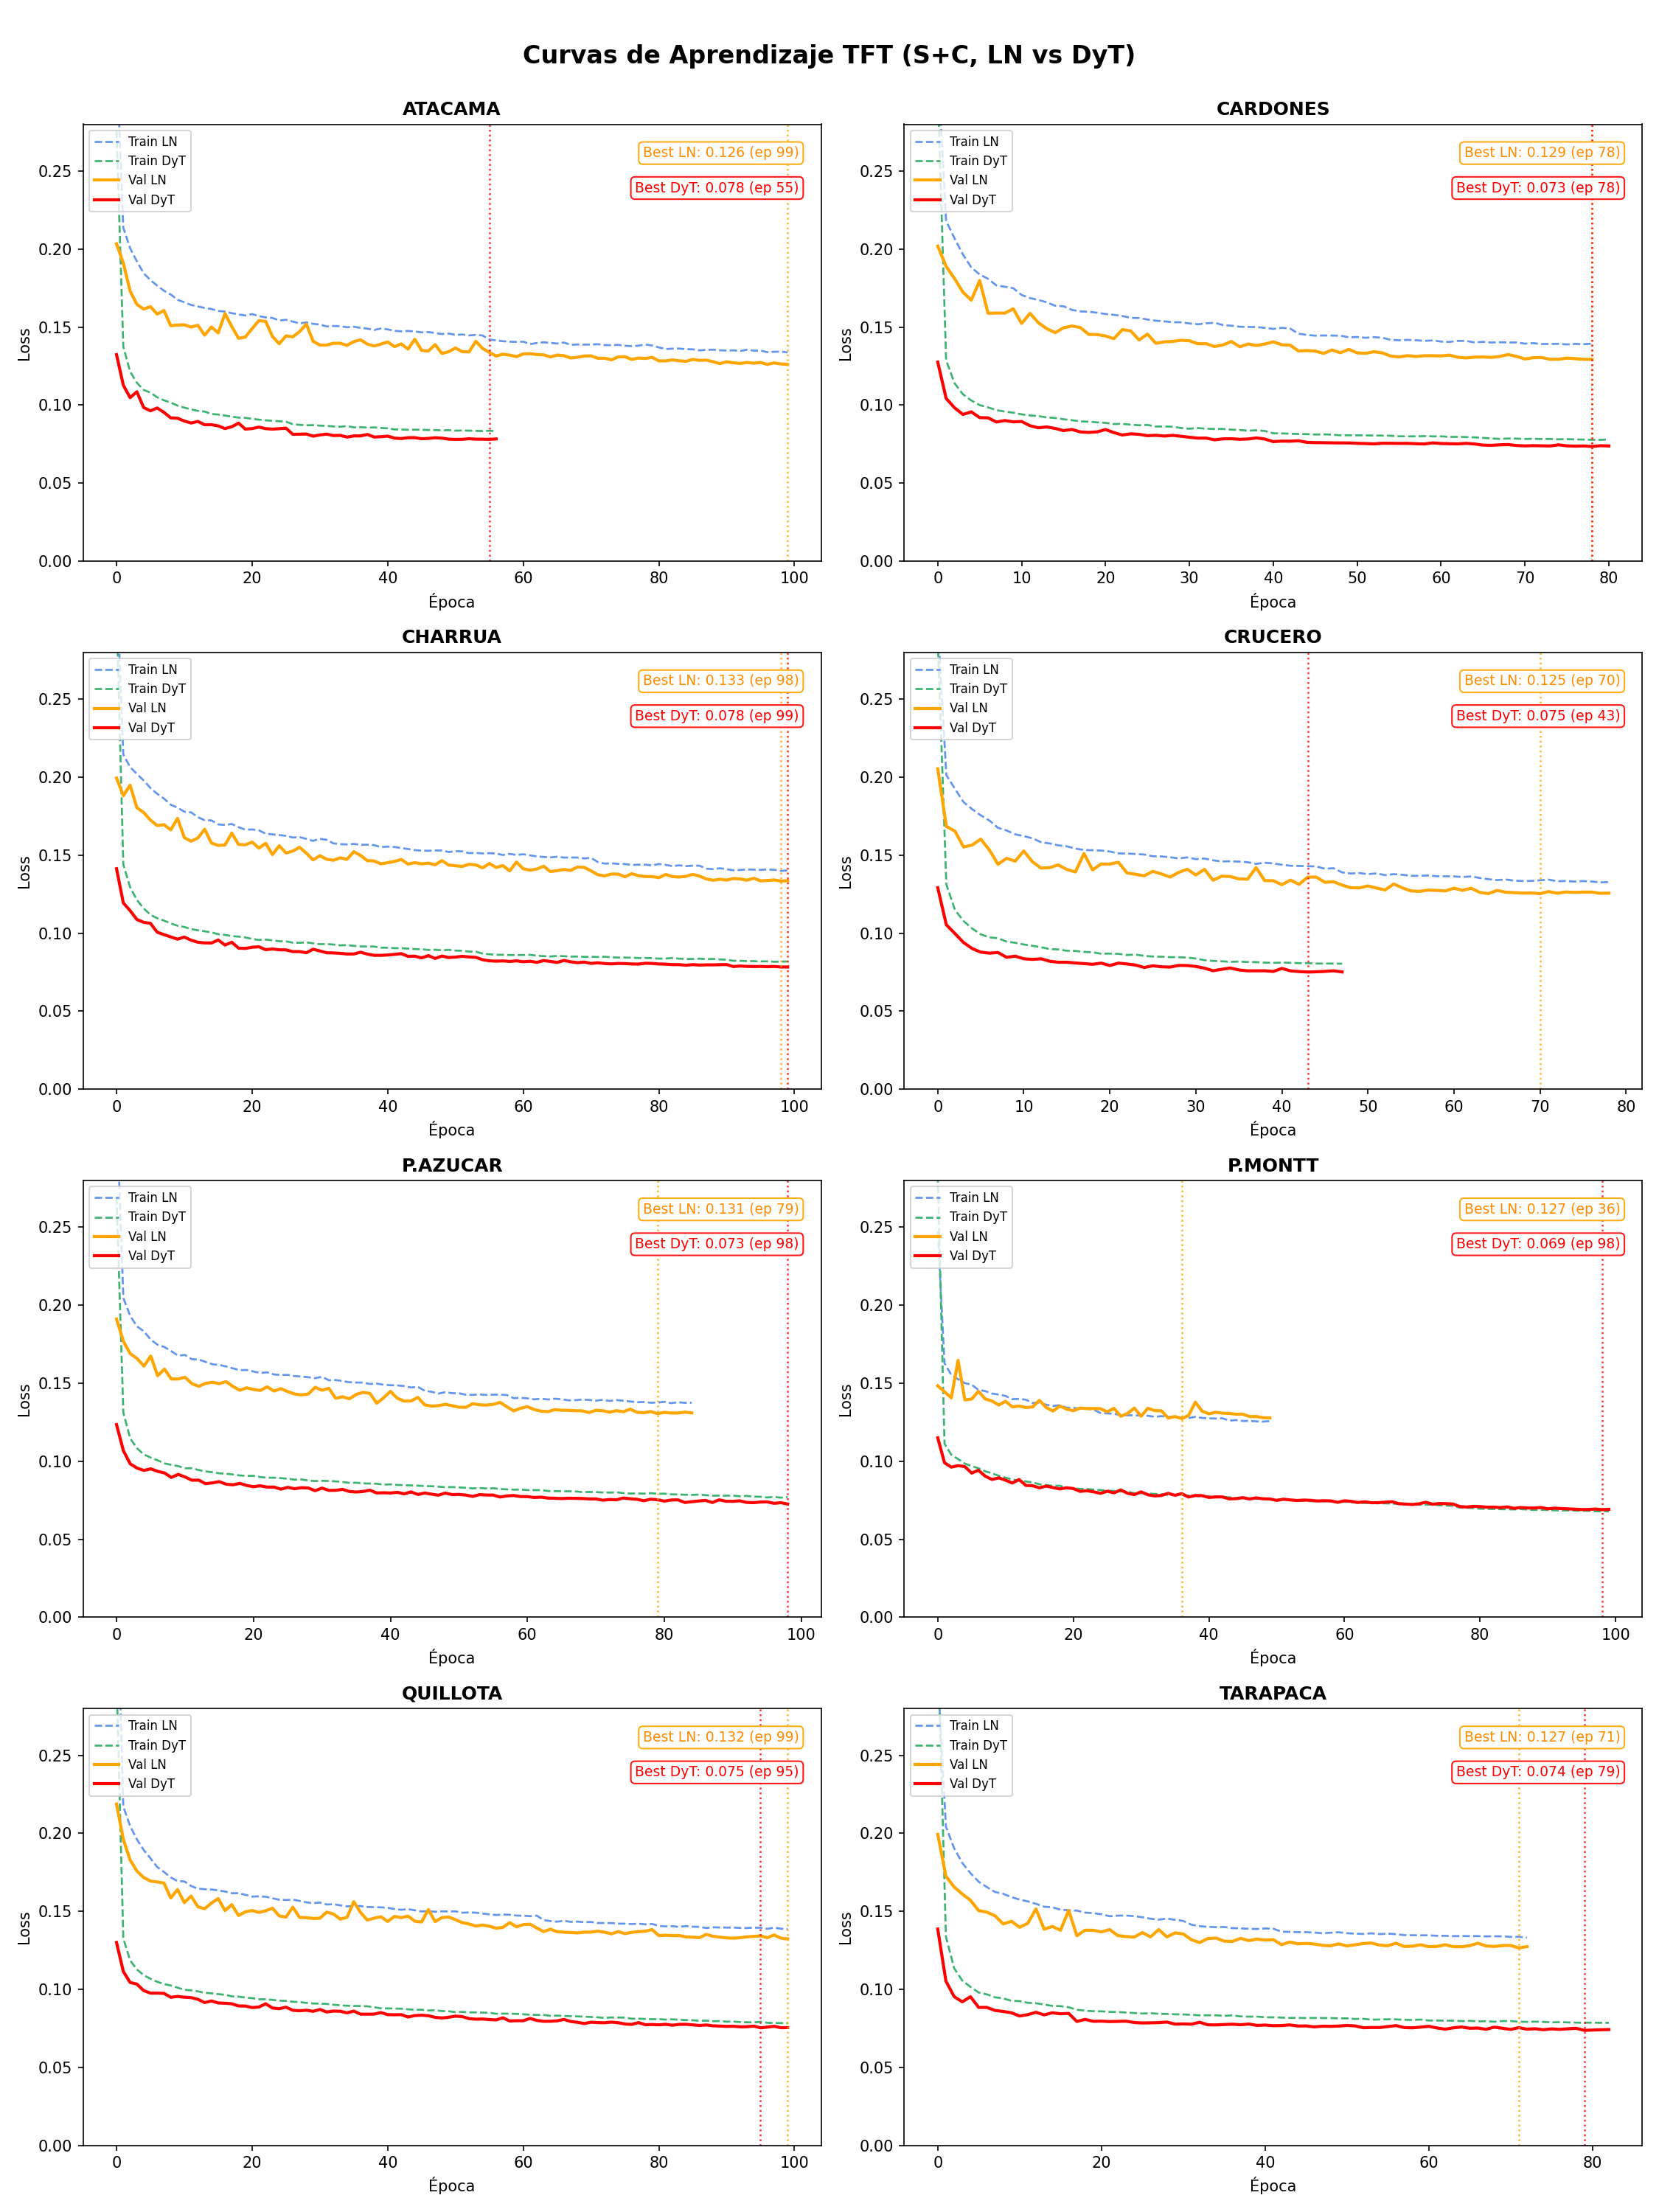
\includegraphics[width=0.95\textwidth]{imagenes/Posibles img/Curvas Aprendizaje SC.png}
    \caption{Curvas de aprendizaje de la rama S+C para las ocho barras del SEN, comparando $\text{TFT}_\text{LN}$ y $\text{TFT}_\text{DyT}$. Se muestra la pérdida (MAE) de entrenamiento y validación. Las líneas verticales indican la época de mejor desempeño en validación.}
    \label{fig:sc_learning_curves}
\end{figure}

Al igual que en P+C, ambas arquitecturas muestran convergencia estable sin señales de sobreajuste en S+C. La pérdida de validación de $\text{TFT}_\text{LN}$ converge en torno a 0.125--0.133, y la de $\text{TFT}_\text{DyT}$ alrededor de 0.069--0.078, magnitudes consistentes con las observadas en P+C (Secciones 3.4.3 y 3.6.1) para cada arquitectura respectivamente. La mayoría de los modelos alcanza su mejor desempeño en épocas avanzadas del entrenamiento, aunque con mayor variabilidad entre barras que en P+C; Puerto Montt es nuevamente el caso más temprano ($\text{TFT}_\text{LN}$, época 36), consistente con su mayor volatilidad estructural ya documentada en la Sección 3.1.

\section{Conformal Prediction}

La Predicción Conforme se aplica sobre la predicción puntual de S+C-LN, la estrategia de referencia seleccionada en la Sección 4.4.5, con el objetivo de construir intervalos de cobertura garantizada para cada barra. En esta sección se describe la configuración del esquema de calibración y las cinco variantes implementadas sobre S+C-LN, más CQR como comparación externa; los resultados se presentan en el Capítulo 4.

\subsection{Configuración general}
\label{sec:cp_configuracion_general}

Todas las variantes se evalúan con nivel de cobertura nominal $1 - \alpha = 0.95$ y operan sobre la escala original de los costos marginales en USD/MWh. El conjunto de calibración es el conjunto de validación descrito en la Tabla \ref{tab:division}, que cubre el período junio 2024--mayo 2025 con $n_{\text{cal}} = 8\,298$ observaciones por barra; el conjunto de evaluación es el conjunto de prueba, con $n_{\text{test}} = 8\,298$ observaciones horarias por barra, cubriendo mayo 2025--abril 2026. Se excluye del conjunto de calibración una ventana de 11 horas (25--26 de febrero de 2025) en la que las ocho barras registraron simultáneamente el mismo valor exacto (576.82\,USD/MWh): un precio de falla administrativo aplicado uniformemente a todo el sistema, no un precio de mercado dependiente de las variables que el modelo puntual utiliza como predictores (Sección \ref{sec:split_cp_clasico}). El límite inferior de todos los intervalos, sin excepción, se trunca en 0 USD/MWh para respetar el dominio físico del costo marginal; el truncamiento no altera la cobertura empírica reportada, solo reduce el ancho medio en la magnitud correspondiente a la porción del intervalo que caía por debajo de 0 antes de truncar (Sección \ref{sec:split_cp_clasico}).

Los \textit{scores} de no conformidad utilizados en todas las variantes son los residuos absolutos del modelo de predicción puntual:

\begin{equation}
    s_t = \lvert y_t - \hat{y}_t \rvert,
    \label{eq:nonconformity}
\end{equation}

donde $\hat{y}_t$ es la predicción puntual cruda de S+C-LN para la barra correspondiente, la misma para las cinco variantes implementadas: usar un único predictor puntual es necesario para que el ancho de intervalo resultante sea comparable entre métodos (Sección \ref{sec:lwacp_comparativa}), ya que cambiar el modelo base de un método a otro confundiría el efecto propio de cada mecanismo de calibración con el efecto de un predictor distinto. Los intervalos resultantes son simétricos alrededor de $\hat{y}_t$:

\begin{equation}
    C_t = \bigl[\,\hat{y}_t - q_t,\; \hat{y}_t + q_t\,\bigr],
    \label{eq:interval}
\end{equation}

donde $q_t$ es el cuantil adaptado por cada método en el instante $t$. Las métricas de evaluación son la cobertura empírica (\textit{Coverage}), el ancho medio del intervalo (\textit{Width}) y el MAE de la predicción puntual subyacente.

Cabe señalar una limitación metodológica del esquema de calibración adoptado. El conjunto de validación cumple un doble rol: primero, participa en la selección del punto de early-stopping del entrenamiento del TFT (Sección 3.4.2); segundo, se utiliza como conjunto de calibración para estimar el cuantil de no conformidad. Esto puede producir un cuantil $q$ ligeramente subestimado respecto al que se obtendría sobre datos completamente independientes, ya que el modelo fue implícitamente seleccionado para desempeñarse bien sobre ese mismo conjunto. La solución ideal sería un tercer conjunto dedicado exclusivamente a calibración, pero con datos de series de tiempo esto reduce el tamaño de calibración disponible. Con $n_{\text{cal}} = 8\,298$ observaciones el sesgo es probablemente pequeño dado el tamaño del conjunto, y se reporta como limitación del diseño experimental.

\subsection{Split CP clásico}

El Split CP clásico, descrito en la Sección 2.6.1, calcula un cuantil fijo $q$ a partir del conjunto de calibración y lo aplica sin cambios a todo el período de prueba. Formalmente, dados los \textit{scores} de calibración $\{s_i\}_{i=1}^{n_{\text{cal}}}$ definidos en \eqref{eq:nonconformity}, el cuantil se obtiene como

\begin{equation}
    q = \hat{Q}_{1-\alpha}\!\left(\{s_i\}_{i=1}^{n_{\text{cal}}}\right),
    \quad
    \text{con nivel ajustado }
    \frac{\lceil (1-\alpha)(n_{\text{cal}}+1)\rceil}{n_{\text{cal}}+1},
    \label{eq:scp_quantile}
\end{equation}

garantizando cobertura marginal finita cuando las observaciones son intercambiables (Vovk et al., 2005) \cite{VovkCP}.

\subsection{ACI}
\label{sec:aci_metodologia}

La \textit{Adaptive Conformal Inference} (ACI), propuesta por Gibbs y Candès (2021) y descrita en la Sección 2.6.4, adapta el nivel de cobertura efectivo $\alpha_t$ en cada instante según la historia reciente de errores de cobertura, sin modificar el \textit{score} de no conformidad ni el modelo de predicción puntual, que es el mismo $\hat{y}_t$ de S+C-LN usado por Split CP, LW Split CP y LW-ACP. El nivel evoluciona según la regla de actualización

\begin{equation}
    \alpha_{t+1} = \alpha_t + \gamma\,(\alpha - \mathbf{1}_{\{y_t \notin C_t\}}),
    \label{eq:aci_update_metodologia}
\end{equation}

donde $\gamma = 0.05$, fijado de antemano e igual al usado en LW-ACP (Sección \ref{sec:lwacp}), en vez de compararse varios valores de $\gamma$ y reportar el de mejor desempeño en el conjunto de prueba; $\alpha = 0.05$ es el nivel nominal. Formalmente, en cada paso $t$ del conjunto de prueba: se calcula el cuantil $q_t$ de los \textit{scores} de calibración con nivel $1-\alpha_t$, se construye $C_t = [\hat{y}_t - q_t,\, \hat{y}_t + q_t]$, se observa $y_t$ y se actualiza $\alpha_{t+1}$ según \eqref{eq:aci_update_metodologia}. Al no reajustarse ningún modelo de predicción en cada paso --solo el escalar $\alpha_t$--, ACI no distingue entre una variante \textit{offline} y una \textit{online} como en formulaciones que sí incorporan un modelo auxiliar reentrenable: es un único método, con un costo computacional equivalente al de Split CP más la actualización escalar de $\alpha_t$ en cada instante.

\subsection{LW Split CP}

La \textit{Locally-Weighted Split CP} (LW Split CP), descrita en la Sección \ref{sec:lwacp}, reemplaza el score de no conformidad absoluto \eqref{eq:nonconformity} por su versión normalizada por hora del día:

\begin{equation}
    \tilde{s}_i = \frac{s_i}{\hat{\sigma}_{h(i)}}, \qquad i \in \mathcal{C}al
    \label{eq:lw_score_metodologia}
\end{equation}

donde $\hat{\sigma}_h$ es la desviación estándar de los residuos absolutos de calibración de la hora $h$, estimada según \eqref{eq:sigma_h} con un mínimo de 30 observaciones por hora; si alguna hora no alcanza ese mínimo, se usa la desviación estándar global de calibración como respaldo. Con $n_{\text{cal}} = 8\,298$ observaciones repartidas en 24 horas, cada hora dispone en promedio de $346$ observaciones, muy por sobre el umbral mínimo. Adicionalmente, $\hat{\sigma}_h$ se acota inferiormente por la desviación estándar global de calibración ($\hat{\sigma}_h \geq \hat{\sigma}_{\text{global}}$): sin este piso, en horas de variabilidad intrínsecamente baja un único \textit{score} de calibración inusualmente grande, al normalizarse por un $\hat{\sigma}_h$ casi nulo, produce un \textit{score} normalizado extremo que infla el cuantil $q$ para todas las horas, no solo la afectada --efecto verificado empíricamente en dos de las ocho barras (Sección \ref{sec:lw_split_cp})--. El cuantil $q$ se calcula sobre los scores normalizados $\{\tilde{s}_i\}$ con la misma corrección de muestra finita de \eqref{eq:scp_quantile}, y el intervalo en cada instante de prueba se reescala por la desviación local de esa hora: $C_t = [\hat{y}_t - q\,\hat{\sigma}_{h(t)},\; \hat{y}_t + q\,\hat{\sigma}_{h(t)}]$.

\subsection{LW-ACP Online}

La \textit{Locally-Weighted Adaptive Conformal Prediction} (LW-ACP), descrita en la Sección \ref{sec:lwacp}, combina la normalización por hora de \eqref{eq:lw_score_metodologia} con la actualización online del nivel de cobertura de ACI \eqref{eq:aci_update_metodologia}. El conjunto de scores normalizados de calibración $\{\tilde{s}_i\}_{i \in \mathcal{C}al}$ se calcula una única vez, igual que en LW Split CP; lo que varía en cada paso $t$ del conjunto de prueba es el nivel de cobertura efectivo $\alpha_t$, que determina un cuantil distinto en cada instante:

\begin{equation}
    q_t = \hat{Q}_{1-\alpha_t}\!\left(\{\tilde{s}_i\}_{i \in \mathcal{C}al}\right), \qquad
    C_t = \left[\hat{y}_t - q_t\,\hat{\sigma}_{h(t)},\; \hat{y}_t + q_t\,\hat{\sigma}_{h(t)}\right]
\end{equation}

Tras observar $y_t$, se actualiza $\alpha_{t+1} = \alpha_t + \gamma\,(\alpha - \mathbf{1}_{\{y_t \notin C_t\}})$, con $\alpha_{t+1}$ acotado al intervalo $[0.001,\, 0.999]$ para evitar niveles degenerados. Se utiliza $\gamma = 0.05$, fijado de antemano e igual al usado en ACI (Sección \ref{sec:aci_metodologia}), en vez de compararse varios valores de $\gamma$ y reportar el de mejor desempeño en el conjunto de prueba. Al igual que ACI, LW-ACP no reajusta ningún modelo de predicción en cada paso: el modelo puntual $\hat{y}_t$ es la predicción cruda de S+C-LN, ya calculada y fija durante todo el período de prueba, y el conjunto de calibración tampoco se actualiza. El único componente dinámico es $\alpha_t$; la diferencia entre ambos métodos es exclusivamente la normalización por hora del \textit{score} de no conformidad \eqref{eq:lw_score_metodologia}, presente en LW-ACP y ausente en ACI.

\subsection{CQR (Regresión Cuantílica Conformada)}

CQR (Sección 2.6.2) se emplea en este trabajo como método de comparación externo a la familia de Conformal Prediction, evaluado, al igual que las cinco variantes anteriores, sobre las ocho barras de S+C-LN, usando en cada caso la predicción puntual de S+C-LN como $\hat{y}_t$.

Los cuantiles $\hat{q}_{\alpha/2}$ y $\hat{q}_{1-\alpha/2}$ de la Sección 2.6.2 se estiman mediante \texttt{QuantileRegressor} de \texttt{scikit-learn} (regresión lineal con penalización $\ell_1$, $\lambda = 0.01$), ajustados sobre tres \textit{features}: la predicción puntual $\hat{y}_t$ y las componentes $\sin(2\pi h_t/24)$, $\cos(2\pi h_t/24)$ de la hora del día. La calibración se realiza sobre el conjunto de validación mediante \textit{K-fold cross-conformal} con $K=5$ pliegues sin mezclar el orden temporal: en cada pliegue se ajustan los modelos cuantílicos sobre los $K-1$ pliegues restantes y se calculan los \textit{scores} \eqref{eq:cqr_score} sobre el pliegue retenido; los scores de los cinco pliegues se acumulan antes de calcular el cuantil corregido $\hat{q}_{1-\alpha}(\mathcal{S})$ con la misma corrección de muestra finita de \eqref{eq:scp_quantile}. Esta variante cross-conformal se prefirió sobre un único split temporal fijo dentro de la validación porque, en pruebas preliminares, el desfase de distribución entre la primera y la segunda mitad del conjunto de validación inflaba artificialmente $\hat{q}_{1-\alpha}(\mathcal{S})$; acumular scores de los cinco pliegues produce una estimación más estable de la calibración. Los modelos cuantílicos finales, usados para predecir sobre el conjunto de prueba en \eqref{eq:cqr_interval}, se reajustan sobre el conjunto de validación completo. El límite inferior del intervalo se trunca en 0 USD/MWh, igual que en las demás variantes de CP (Sección \ref{sec:cp_configuracion_general}), y se corrige el orden de los límites en los casos infrecuentes en que el límite inferior supera al superior.

\section{Extensiones y análisis complementarios}

Además de la comparación central entre las estrategias P+C y S+C, se realizan los siguientes análisis complementarios: un tratamiento diferenciado de Puerto Montt con features hídricas propias, una comparación contra el costo marginal programado del CEN, una evaluación de sensibilidad frente a una función de pérdida asimétrica, un estudio preliminar del efecto de la granularidad temporal, un estudio de ablación de features, un piloto de entrenamiento sin recorte de outliers, una evaluación a horizonte \textit{day-ahead} ($h=24$), y una comparación con resultados reportados en la literatura reciente para las barras Crucero y Puerto Montt. Los resultados de estas extensiones se presentan en el Capítulo 4.

\subsection{Puerto Montt: features hídricas (H+C y S+H+C)}

Puerto Montt exhibe sistemáticamente el peor desempeño del sistema bajo P+C y S+C, consistente con su mayor media y desviación estándar de costo marginal (Tabla \ref{tab:estadisticas}). Para evaluar si esto se debe a la ausencia de una señal específica de la dinámica hidroeléctrica de la zona centro-sur, se entrenan dos estrategias adicionales exclusivamente para esta barra.

\textbf{H+C (Hídrico + Clima):} sin \texttt{known\_reals} (ni componentes de Prophet ni posición solar), con \texttt{unknown\_reals} compuestas por las cinco variables climáticas ya descritas (Sección 3.4.1) más dos variables hídricas propias de la cuenca que alimenta Canutillar, la principal central hidroeléctrica que abastece esta barra: \texttt{cota\_chapo}, la cota del embalse Lago Chapo en metros sobre el nivel del mar, y \texttt{agua\_caida\_hora}, el agua caída diaria del sistema Canutillar en milímetros. Ambas variables se obtienen originalmente a frecuencia diaria (la cota como promedio diario de lecturas horarias, el agua caída como medición diaria directa) y se expanden a resolución horaria repitiendo el valor del día correspondiente en sus 24 horas, dado que ambas evolucionan en escalas de tiempo mucho más lentas que el costo marginal horario. Esta expansión introduce la misma limitación de viabilidad operacional señalada para las variables climáticas (Sección 3.4.1): si el valor diario de \texttt{agua\_caida\_hora} corresponde a una medición o acumulado cerrado al final del día $d$, repetirlo desde las 00:00 de $d$ supone disponer, en la hora 00:00, de información que en la práctica solo se conoce al término de ese mismo día. El esquema es internamente consistente para el entrenamiento y la evaluación --el valor diario ya observado se usa igual en todas las horas de ese día, sin mirar días futuros--, pero un despliegue operacional en tiempo real requeriría, análogamente al caso climático, sustituir el valor diario cerrado por una estimación disponible a esa hora (por ejemplo, el último valor diario ya cerrado, con un día de rezago, en vez del valor del día en curso).

\textbf{S+H+C (Sol + Hídrico + Clima):} idéntica a H+C, pero agregando las tres variables solares \texttt{known\_reals} de S+C (Sección 3.4.1). Esta variante se introduce para evaluar si la ausencia de una señal cíclica explícita que H+C no tiene, a diferencia de P+C y S+C explica su desempeño.

Ambas estrategias entrenan una única instancia del TFT (sin residuos de Prophet ni Stacking Optimization posterior), con los mismos hiperparámetros, ventana de contexto y horizonte que el resto del pipeline (Tabla \ref{tab:tft_config}), y se comparan contra P+C (mejor estrategia de Stacking Optimization para P.Montt, Sección 3.5) y S+C (TFT de precios solo) mediante MAE/RMSE/R² y el test de Diebold-Mariano (1995) sobre los errores absolutos horarios pareados, con la varianza de la diferencia de pérdidas estimada vía Newey-West para tolerar la autocorrelación serial del error horario, para determinar si las diferencias observadas son estadísticamente significativas.

\subsection{Comparación contra el costo marginal programado del CEN}

Se incorpora además una línea base institucional: el \textit{costo marginal programado} que el CEN publica operacionalmente como resultado de la Programación de la Operación, obtenido sobre las 8\,298 horas del conjunto de prueba mediante la API pública del Sistema de Información Pública del CEN (\texttt{sipub.coordinador.cl}), identificando cada nodo mediante su mnemotécnico de barra en el catálogo de la API (por ejemplo, \texttt{BA01T0002SE031T0002} para Puerto Montt, S/E Puerto Montt 220kV BP2) y agregando los registros de 15 minutos u horarios disponibles a resolución horaria. El mnemotécnico correcto se logró identificar, probando las variantes de voltaje y sección de barra disponibles en el catálogo, para seis de las ocho barras: Puerto Montt, Cardones, Charrúa, Crucero, Pan de Azúcar y Quillota. Para Atacama y Tarapacá no se encontró ningún mnemotécnico de barra 220kV con datos disponibles en este recurso de la API, en ningún período consultado.

\subsection{Sensibilidad a una función de pérdida asimétrica}

Como cierre aplicado, se evalúa si la ventaja de S+C-LN sobre la línea base de persistencia (Sección 4.1) se sostiene bajo una función de pérdida asimétrica, en vez de las métricas simétricas (MAE, RMSE) usadas en el resto de este trabajo. Se emplea la pérdida lineal-lineal (\textit{linlin} o \textit{pinball}) con parámetro $\tau \in (0,1)$, $L_\tau(e) = \tau \max(e,0) + (1-\tau)\max(-e,0)$ con $e = y_t - \hat{y}_t$, que penaliza la subestimación del precio ($e>0$) con peso $\tau$ y la sobreestimación ($e<0$) con peso $1-\tau$; $\tau=0.5$ recupera el caso simétrico. Se calcula $L_\tau$ para S+C-LN y para la persistencia (Sección 4.1) sobre el conjunto de prueba de las ocho barras, para $\tau \in \{0.2, 0.35, 0.5, 0.65, 0.8\}$, y se reporta el \textit{skill score} $1 - L_\tau(\text{S+C-LN})/L_\tau(\text{persistencia})$ para cada valor de $\tau$.

\subsection{Estudio de granularidad temporal}

Para explorar si una resolución temporal distinta a la horaria mejora la capacidad predictiva del modelo, se reentrena la estrategia ganadora S+C a dos resoluciones adicionales para tres barras piloto (Atacama, Cardones, P.Montt) y ambas arquitecturas (LN, DyT): \textbf{Día}, agregando el costo marginal horario a promedio diario, y \textbf{15 minutos}, usando el costo marginal a resolución nativa de 15 minutos del CEN. En ambos casos se mantiene la misma arquitectura, hiperparámetros y proporción de encoder/predicción (168 pasos de contexto, horizonte de 1 paso), reinterpretando la unidad temporal según la granularidad: 168 días de contexto para Día, 168 intervalos de 15 minutos (42 horas) para 15 minutos.

Esta comparación tiene una limitación metodológica relevante: los tres experimentos cubren períodos históricos distintos y no completamente superpuestos, dado que la disponibilidad de datos crudos difiere por granularidad (Día: 2020--2025; Horario: 2020--2026; 15 minutos: solo ~2024--2026, con datos de 15 minutos disponibles a partir de mediados de 2024). Para aislar el efecto de la resolución del efecto del período histórico, se entrena un cuarto modelo adicional: \textbf{Horario restringido a la ventana calendario del piloto de 15 minutos} (train/val hasta el 16 de marzo de 2026, test entre el 16 de marzo y el 24 de abril de 2026, truncado por la disponibilidad de datos crudos de precio), que permite comparar Horario y 15 minutos sobre exactamente el mismo período, recortando también el test del piloto de 15 minutos original a esa misma ventana.

\subsection{Ablación de features}

Para aislar cuánto aporta la información exógena (posición solar y clima) por sobre la autocorrelación de la propia serie, se entrena una variante "solo precios" del TFT (sin ningún \texttt{known\_real} ni variable climática, únicamente la serie de costo marginal estandarizada como \texttt{unknown\_real}) para cuatro barras (Atacama, Cardones, P.Montt, Tarapaca), usando el mismo período histórico y las mismas fechas de corte train/val/test que el pipeline principal (Tabla \ref{tab:division}), de modo que la única diferencia respecto de S+C sea la presencia o ausencia de las features exógenas.

\subsection{Piloto: entrenamiento sin recorte de outliers}
\label{sec:piloto_outliers_meta}

El recorte automático de outliers descrito en la Sección 3.2.1 (umbral de 4 desviaciones estándar sobre el conjunto de entrenamiento) se diseñó para eliminar valores de magnitud excepcional sin afectar los \textit{spikes} estructurales del mercado. Una inspección posterior del conjunto de entrenamiento sugirió que, en varias barras, ese umbral recorta no solo eventos aislados sino un patrón sostenido en el tiempo, concentrado en el invierno de 2022 --varias semanas de precios altos, no observaciones puntuales--, lo que plantea la posibilidad de que parte de la señal removida sea información legítima sobre el régimen de precios altos y no ruido de medición.

Para evaluar esta hipótesis se entrena un piloto de S+C-LN sin el recorte automático de outliers en el conjunto de entrenamiento --Validación y Prueba ya se evaluaban contra la serie cruda desde el pipeline principal (Sección \ref{sec:baselines})--, para cuatro barras (Atacama, Charrúa, Pan de Azúcar, Tarapacá). La única exclusión manual retenida corresponde a tres horas de Pan de Azúcar (19 de marzo de 2020, 17--19h, valores entre 860 y 1589 USD/MWh frente a una media de la barra de aproximadamente 71 USD/MWh), un error de medición aislado y verificable, no un patrón de mercado. El modelo Prophet de la rama P+C se reentrena también con este nuevo conjunto de entrenamiento para las mismas cuatro barras; el resto del pipeline (clima, posición solar, hiperparámetros) permanece idéntico al modelo principal.

El piloto se evalúa a $h=1$ (idéntico al pipeline principal) y a $h=24$ (idéntico a la Sección \ref{sec:h24_dayahead}), para determinar si el efecto del recorte de outliers depende del horizonte de predicción. Además del MAE general de prueba, se reporta el MAE condicional al régimen de precio alto (percentil 95 o superior de la serie cruda de prueba), el régimen que la hipótesis del recorte sistemático busca capturar mejor.

\subsection{Evaluación a horizonte \textit{day-ahead} ($h=24$)}
\label{sec:h24_dayahead_meta}

El pipeline principal de este trabajo adopta un horizonte $h=1$ hora (Sección 3.4.2), pero el horizonte operacionalmente más relevante en mercados eléctricos es el \textit{day-ahead} ($h=24$, Sección 2.3.3). Para evaluar si S+C-LN generaliza a ese horizonte sin modificaciones adicionales al pipeline, se reentrena con \texttt{max\_prediction\_length=24} (estrategia MIMO, Sección 2.3.3), reutilizando el mismo \texttt{datasets\_norm} y \texttt{scalers} ya calculados para $h=1$ sin recomputar features climáticas ni solares, para cinco barras (Atacama, Charrúa, Pan de Azúcar, Puerto Montt, Tarapacá) y ambas arquitecturas, manteniendo el resto de los hiperparámetros de la Tabla \ref{tab:tft_config} sin cambios --ninguno de ellos se reoptimiza específicamente para este horizonte, la misma limitación de esfuerzo de ajuste asimétrico señalada en la Sección \ref{sec:ln_vs_dyt}--.

Cada uno de los 24 pasos del horizonte se extrae de una única pasada de inferencia sobre el conjunto de prueba y se compara contra una línea base de persistencia estacional de 24 horas (el mismo valor observado 24 horas antes, Sección \ref{sec:baselines}), reportando MASE y \textit{skill score} promediados sobre los 24 pasos, además de la degradación del MAE entre el primer y el último paso del horizonte.

Como seguimiento acotado a este resultado, se evalúa además si aumentar la capacidad del modelo --duplicando \texttt{hidden\_size} (32→64) y \texttt{hidden\_continuous\_size} (8→16), sin modificar ningún otro hiperparámetro-- atenúa la degradación observada, para dos barras (Atacama y Puerto Montt, la de mejor y peor desempeño del pipeline principal, respectivamente), dado el costo computacional de este experimento adicional (aproximadamente 4 horas por barra en GPU para el modelo de mayor capacidad, medido directamente).

\subsection{Comparación con la literatura: Crucero y P.Montt 2024}

León et al. (2026) \cite{LeonSMPChile}, ya presentado en la Sección 1.1, comparan modelos de \textit{machine learning} clásico para predecir el costo marginal horario del SEN en tres barras representativas, usando datos de 2024 y evaluación \textit{holdout} sobre enero y julio. Para una comparación aproximada con ese trabajo, se entrenan dos modelos S+C adicionales restringidos a datos de 2024, para las barras Crucero y P.Montt, dos de las tres barras representativas de León et al., y ambas también estudiadas en profundidad en este trabajo (Sección 3.8.1), cada una con un split cronológico propio 70/15/15 (en vez de las fechas de corte de la Tabla \ref{tab:division}, que exceden el rango de un año), manteniendo el resto de la configuración idéntica al pipeline principal.
\chapter{Resultados y Análisis}

Este capítulo presenta los resultados de evaluación del modelo híbrido propuesto, organizados siguiendo el orden de la arquitectura descrita en el Capítulo 3: primero los modelos base individuales (Prophet y TFT), luego el Stacking Optimization, y finalmente los intervalos de Conformal Prediction. Para cada componente se reportan las métricas en los conjuntos de validación y prueba, y se identifican los patrones transversales entre barras. Las comparativas entre arquitecturas ($\text{TFT}_\text{LN}$ vs.\ $\text{TFT}_\text{DyT}$) y entre métodos de CP se presentan al final de cada sección correspondiente.

\section{Líneas base ingenuas}
\label{sec:baselines}

Antes de presentar los modelos propuestos, se establecen líneas base ingenuas sobre la misma serie cruda y el mismo conjunto de prueba usado en el resto del capítulo, para poder interpretar las cifras de error absolutas que siguen. Se evalúan cinco referencias por barra: persistencia (predecir el valor de la hora anterior, $\hat{y}_t = y_{t-1}$), naive estacional a un día ($\hat{y}_t = y_{t-24}$) y a una semana ($\hat{y}_t = y_{t-168}$), y dos modelos autorregresivos AR(24) y AR(168) ajustados por mínimos cuadrados ordinarios (OLS) sobre el conjunto de entrenamiento, de la forma $\hat{y}_t = a\,y_{t-\ell} + b$ con $\ell \in \{24, 168\}$. Ninguna de estas referencias requiere entrenar el TFT ni ningún otro componente del \textit{pipeline}. La Tabla \ref{tab:baselines_naive} presenta los resultados.

\begin{table}[htbp]
    \centering
    \small
    \begin{tabular}{lrrrrr}
        \toprule
        Barra & Persistencia & Naive-24h & Naive-168h & AR(24) & AR(168) \\
        \midrule
        Atacama       & 10.35 & 12.35 & 15.07 & 16.21 & 20.29 \\
        Cardones      & 10.34 & 12.77 & 15.71 & 16.39 & 20.63 \\
        Charrúa       & 10.28 & 19.14 & 22.96 & 21.35 & 25.52 \\
        Crucero       & 10.43 & 12.48 & 15.22 & 16.16 & 20.19 \\
        Pan de Azúcar & 10.38 & 13.16 & 16.22 & 17.65 & 22.19 \\
        Puerto Montt  & 14.20 & 37.33 & 43.89 & 39.25 & 46.18 \\
        Quillota      & 10.40 & 19.18 & 22.83 & 21.20 & 25.27 \\
        Tarapacá      & 11.06 & 13.08 & 15.99 & 16.88 & 21.13 \\
        \bottomrule
    \end{tabular}
    \caption{MAE (USD/MWh) de las líneas base ingenuas sobre la serie cruda, evaluadas en el mismo conjunto de prueba que el resto del capítulo, las ocho barras del SEN.}
    \label{tab:baselines_naive}
\end{table}

La persistencia de un paso es, en las ocho barras, la línea base más difícil de superar: a resolución horaria, el precio de la hora inmediatamente anterior es más informativo que el mismo momento del día anterior o de la semana anterior, y también más informativo que los modelos AR(24) y AR(168) ajustados por OLS, que resultan sistemáticamente peores que el naive del que parten. Esto se explica porque el ajuste por mínimos cuadrados minimiza el error cuadrático, lo que produce coeficientes menores a uno y un intercepto positivo que suaviza la predicción hacia la media --óptimo para el error cuadrático, pero no para el error absoluto sobre una serie con una masa puntual considerable en cero y una cola derecha pesada--. Por este motivo, se adopta la persistencia de un paso como referencia para el \textit{skill score} y el MASE (\textit{Mean Absolute Scaled Error}, Hyndman y Koehler, 2006) reportados junto al modelo de referencia S+C-LN en la Tabla \ref{tab:tft_sc_ln_resultados}: $\text{MASE} = \text{MAE}_{\text{modelo}} / \text{MAE}_{\text{persistencia}}$, y $\text{skill score} = 1 - \text{MASE}$.

\section{Modelo Prophet}
\label{sec:modelo_prophet}

\subsection{Desempeño por barra}

La Figura \ref{fig:prophet_comparativa} presenta la comparativa entre los valores reales y las predicciones de Prophet para las ocho barras sobre el período completo de estudio.

\begin{figure}[htbp]
    \centering
    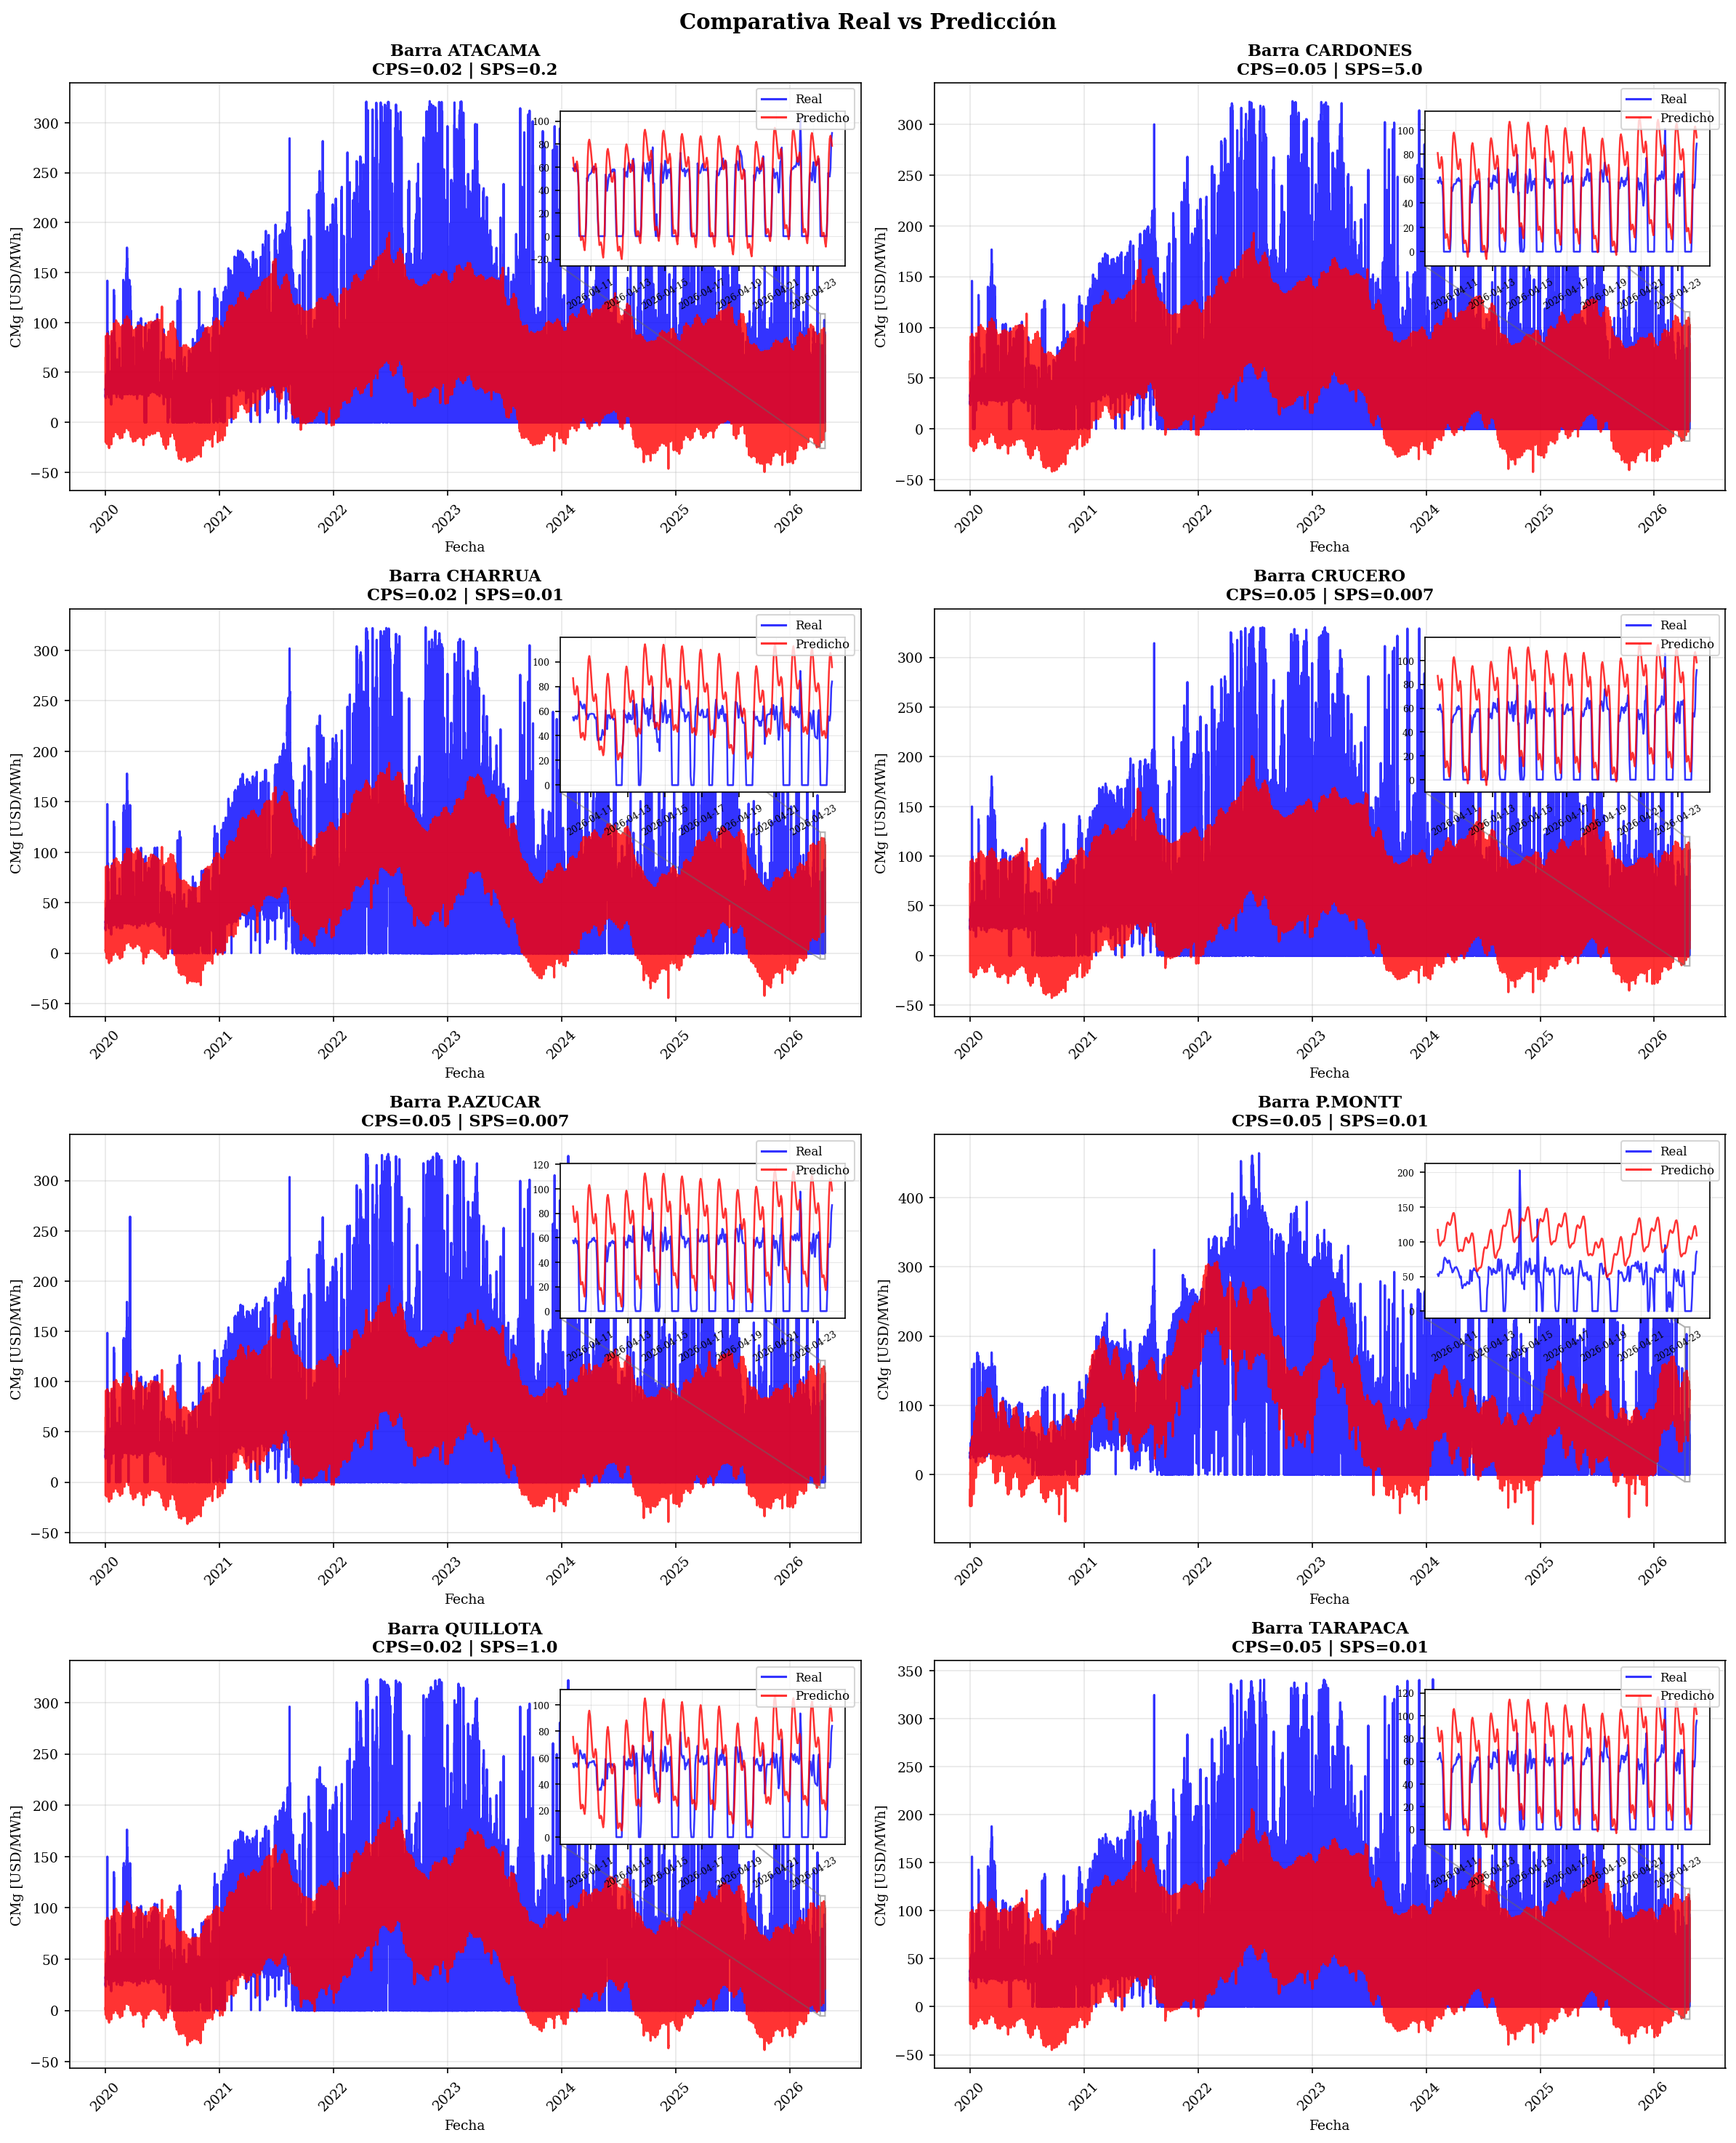
\includegraphics[width=0.95\textwidth]{imagenes/Posibles img/Comparativa Real vs Predicho.png}
    \caption{Comparativa entre valores reales (azul) y predicciones de Prophet (rojo) para las ocho barras del SEN, período 2020--2026.}
    \label{fig:prophet_comparativa}
\end{figure}

La figura ilustra visualmente el comportamiento característico de Prophet como modelo de descomposición: captura adecuadamente la envolvente de la serie, siguiendo la tendencia de largo plazo y los ciclos estacionales, pero suaviza los spikes de alta magnitud que corresponden a eventos extremos del mercado. Este comportamiento es esperable dado que Prophet modela la estructura sistemática de la serie y no está diseñado para capturar fluctuaciones no lineales de corto plazo, rol que corresponde al TFT en la arquitectura híbrida propuesta. Puerto Montt exhibe el mayor desajuste visual, con la predicción incapaz de seguir la alta variabilidad de la serie real durante el período 2022--2023.

La Tabla \ref{tab:prophet_resultados} presenta los resultados numéricos de evaluación de Prophet en los conjuntos de entrenamiento, validación y prueba para las ocho barras.

\begin{table}[htbp]
    \centering
    \small
    \begin{tabular}{llrrrr}
        \toprule
        Barra & Conjunto & MAE & RMSE & MSE & R$^2$ \\
        \midrule
        \multirow{3}{*}{Atacama}
            & Train & 30.40 & 41.05 & 1684.75 &  0.5228 \\
            & Val   & 21.34 & 42.29 & 1788.58 &  0.4023 \\
            & Test  & 16.39 & 28.69 &  823.05 &  0.5264 \\
        \midrule
        \multirow{3}{*}{Cardones}
            & Train & 30.32 & 40.92 & 1674.47 &  0.5314 \\
            & Val   & 21.60 & 37.21 & 1384.42 &  0.4491 \\
            & Test  & 19.95 & 30.09 &  905.28 &  0.4710 \\
        \midrule
        \multirow{3}{*}{Charrúa}
            & Train & 31.58 & 43.61 & 1901.89 &  0.4688 \\
            & Val   & 24.34 & 37.59 & 1412.72 &  0.3225 \\
            & Test  & 24.51 & 37.02 & 1370.68 &  0.3013 \\
        \midrule
        \multirow{3}{*}{Crucero}
            & Train & 30.46 & 41.23 & 1699.97 &  0.5502 \\
            & Val   & 22.83 & 42.13 & 1774.64 &  0.4167 \\
            & Test  & 22.10 & 31.94 & 1019.93 &  0.4238 \\
        \midrule
        \multirow{3}{*}{Pan de Azúcar}
            & Train & 30.83 & 41.98 & 1762.61 &  0.5137 \\
            & Val   & 22.73 & 37.21 & 1384.72 &  0.4161 \\
            & Test  & 22.44 & 31.79 & 1010.37 &  0.4137 \\
        \midrule
        \multirow{3}{*}{Puerto Montt}
            & Train & 50.44 & 67.62 & 4572.02 &  0.5516 \\
            & Val   & 46.00 & 62.88 & 3953.91 &  0.2221 \\
            & Test  & 47.89 & 61.71 & 3808.69 & $-$0.0106 \\
        \midrule
        \multirow{3}{*}{Quillota}
            & Train & 31.24 & 42.88 & 1838.39 &  0.4827 \\
            & Val   & 23.87 & 37.64 & 1416.80 &  0.3401 \\
            & Test  & 23.22 & 36.82 & 1355.75 &  0.3297 \\
        \midrule
        \multirow{3}{*}{Tarapacá}
            & Train & 31.18 & 42.20 & 1780.62 &  0.5568 \\
            & Val   & 23.61 & 43.97 & 1933.03 &  0.4355 \\
            & Test  & 21.86 & 32.88 & 1080.87 &  0.4692 \\
        \bottomrule
    \end{tabular}
    \vspace{0.2cm}
    \caption{Resultados de evaluación de Prophet por barra y conjunto, con las predicciones truncadas en 0 USD/MWh y validación/prueba evaluadas contra la serie cruda. MAE y RMSE en USD/MWh, MSE en (USD/MWh)$^2$.}
    \label{tab:prophet_resultados}
\end{table}

Los resultados muestran un desempeño heterogéneo entre barras. Las barras del norte presentan los mejores indicadores, con R$^2$ en el conjunto de prueba entre 0.41 y 0.53, lo que refleja que Prophet captura adecuadamente la estructura estacional y la tendencia decreciente asociada a la incorporación solar. Quillota y Charrúa muestran un desempeño moderado con R$^2$ de 0.33 y 0.30 respectivamente en prueba, sugiriendo que sus dinámicas de corto plazo son más difíciles de capturar con un modelo de descomposición aditiva. El caso más notable es Puerto Montt, que presenta un R$^2$ negativo de $-0.011$ en el conjunto de prueba, indicando que Prophet es peor que un predictor constante igual a la media para esta barra en el período 2025--2026. Este resultado es consistente con la naturaleza de la generación hidroeléctrica del sur, cuya variabilidad está determinada por ciclos de precipitaciones de baja frecuencia que no siguen patrones estacionales regulares. Este resultado motiva directamente la incorporación del TFT como componente complementario en el ensamble.

Las predicciones de Prophet se truncan en 0 USD/MWh antes de calcular estas métricas, dado que el costo marginal no puede ser negativo (Sección 3.3.3) y Prophet, como modelo de descomposición aditiva sin restricción de dominio, predice valores negativos con frecuencia no despreciable: 29\,346 de las 442\,560 predicciones evaluadas (6.6\%, sumando entrenamiento, validación y prueba en las ocho barras) son negativas antes de truncar. El efecto sobre las métricas es sistemático y no trivial --el MAE de prueba se reduce entre 0.3 (Puerto Montt) y 3.5\,USD/MWh (Atacama), y el R$^2$ de prueba mejora en las ocho barras, con la mayor ganancia en Atacama (0.484 a 0.526)--, consistente con que una fracción relevante de esas predicciones negativas ocurre en las horas de precio real cercano a 0 USD/MWh, donde el error absoluto de una predicción negativa es, por construcción, mayor que el de una predicción truncada en 0. Este truncamiento se aplica únicamente a las métricas de Prophet reportadas en esta sección; no se propaga al residuo que consume $\text{TFT}_\text{LN}$ en la rama P+C, dado que corregir ese residuo exige reentrenar el modelo de residuos sobre el nuevo objetivo, fuera del alcance de esta corrección puntual.

Se observa además una degradación consistente del R$^2$ entre entrenamiento y prueba en todas las barras, lo que es esperable dado el cambio estructural en el mercado eléctrico chileno durante el período de prueba 2025--2026, caracterizado por una mayor penetración renovable y episodios de curtailment más frecuentes que los observados durante el entrenamiento.

\section{Temporal Fusion Transformer con LayerNorm}
 
\subsection{Desempeño por barra}
 
Las Tablas \ref{tab:tft_precios_resultados} y \ref{tab:tft_residuos_resultados} presentan los resultados de evaluación del $\text{TFT}_\text{LN}$ para todas las barras, separados por modelo de precios y de residuos respectivamente.
 
\begin{table}[htbp]
    \centering
    \small
    \begin{tabular}{llrrr}
        \toprule
        Barra & Conjunto & MAE & RMSE & R$^2$ \\
        \midrule
        \multirow{3}{*}{Atacama}
            & Train & 7.81 & 16.30 & 0.925 \\
            & Val   & 8.95 & 29.32 & 0.713 \\
            & Test  & 6.95 & 16.93 & 0.835 \\
        \midrule
        \multirow{3}{*}{Cardones}
            & Train & 7.70 & 16.24 & 0.926 \\
            & Val   & 8.15 & 24.08 & 0.769 \\
            & Test  & 7.02 & 16.11 & 0.848 \\
        \midrule
        \multirow{3}{*}{Charrúa}
            & Train & 8.12 & 16.77 & 0.922 \\
            & Val   & 8.83 & 23.61 & 0.733 \\
            & Test  & 8.52 & 16.12 & 0.868 \\
        \midrule
        \multirow{3}{*}{Crucero}
            & Train & 7.80 & 16.34 & 0.930 \\
            & Val   & 8.80 & 28.50 & 0.733 \\
            & Test  & 7.06 & 16.92 & 0.838 \\
        \midrule
        \multirow{3}{*}{Pan de Azúcar}
            & Train & 7.57 & 15.80 & 0.931 \\
            & Val   & 8.36 & 23.26 & 0.772 \\
            & Test  & 7.17 & 15.33 & 0.864 \\
        \midrule
        \multirow{3}{*}{Puerto Montt}
            & Train & 13.01 & 29.70 & 0.914 \\
            & Val   & 15.80 & 33.19 & 0.783 \\
            & Test  & 13.94 & 25.98 & 0.821 \\
        \midrule
        \multirow{3}{*}{Quillota}
            & Train & 8.10 & 16.66 & 0.922 \\
            & Val   & 8.99 & 23.82 & 0.736 \\
            & Test  & 8.70 & 16.54 & 0.865 \\
        \midrule
        \multirow{3}{*}{Tarapacá}
            & Train & 7.91 & 16.63 & 0.931 \\
            & Val   & 9.17 & 31.08 & 0.718 \\
            & Test  & 7.14 & 17.90 & 0.843 \\
        \bottomrule
    \end{tabular}
    \vspace{0.2cm}
    \caption{Resultados de evaluación del $\text{TFT}_\text{LN}$, modelo de precios (rama P+C), por barra y conjunto, evaluado contra la serie cruda (Val y Test; Train se limpia igual que antes, Sección \ref{sec:baselines}). MAE y RMSE en USD/MWh.}
    \label{tab:tft_precios_resultados}
\end{table}
 
\begin{table}[htbp]
    \centering
    \small
    \begin{tabular}{llrrr}
        \toprule
        Barra & Conjunto & MAE & RMSE & R$^2$ \\
        \midrule
        \multirow{3}{*}{Atacama}
            & Train & 7.61 & 15.65 & 0.857 \\
            & Val   & 8.98 & 28.50 & 0.544 \\
            & Test  & 7.50 & 16.97 & 0.672 \\
        \midrule
        \multirow{3}{*}{Cardones}
            & Train & 7.55 & 15.48 & 0.860 \\
            & Val   & 8.10 & 23.66 & 0.600 \\
            & Test  & 6.80 & 15.39 & 0.736 \\
        \midrule
        \multirow{3}{*}{Charrúa}
            & Train & 8.21 & 16.66 & 0.855 \\
            & Val   & 8.81 & 23.29 & 0.618 \\
            & Test  & 8.46 & 15.62 & 0.823 \\
        \midrule
        \multirow{3}{*}{Crucero}
            & Train & 7.75 & 15.83 & 0.856 \\
            & Val   & 8.99 & 28.62 & 0.540 \\
            & Test  & 7.05 & 16.82 & 0.686 \\
        \midrule
        \multirow{3}{*}{Pan de Azúcar}
            & Train & 8.04 & 16.31 & 0.851 \\
            & Val   & 8.55 & 23.20 & 0.612 \\
            & Test  & 7.22 & 14.92 & 0.757 \\
        \midrule
        \multirow{3}{*}{Puerto Montt}
            & Train & 12.73 & 29.52 & 0.811 \\
            & Val   & 16.08 & 33.28 & 0.718 \\
            & Test  & 14.31 & 26.07 & 0.822 \\
        \midrule
        \multirow{3}{*}{Quillota}
            & Train & 8.28 & 16.60 & 0.851 \\
            & Val   & 9.38 & 23.85 & 0.600 \\
            & Test  & 8.95 & 16.56 & 0.795 \\
        \midrule
        \multirow{3}{*}{Tarapacá}
            & Train & 7.99 & 16.35 & 0.853 \\
            & Val   & 9.31 & 30.39 & 0.526 \\
            & Test  & 7.25 & 17.68 & 0.690 \\
        \bottomrule
    \end{tabular}
    \vspace{0.2cm}
    \caption{Resultados de evaluación del $\text{TFT}_\text{LN}$, modelo de residuos (rama P+C), por barra y conjunto, evaluado contra el residuo reconstruido a partir de la serie cruda (Val y Test; Train se limpia igual que antes, Sección \ref{sec:baselines}). MAE y RMSE en USD/MWh.}
    \label{tab:tft_residuos_resultados}
\end{table}
 
Los resultados muestran una mejora sustancial respecto a Prophet en todas las barras y métricas, evaluados contra la serie cruda (Sección \ref{sec:baselines}). En el $\text{TFT}_\text{LN}$ de precios, el R$^2$ en test oscila entre $0.821$ (Puerto Montt) y $0.868$ (Charrúa), frente a valores de Prophet que iban de $-0.016$ a $0.519$. Para Atacama, el R$^2$ sube de $0.519$ con Prophet a $0.835$ con el modelo de precios. El salto es especialmente pronunciado en Charrúa, de $0.302$ con Prophet a $0.868$ con el $\text{TFT}_\text{LN}$ de precios, y en Puerto Montt, de $-0.016$ a $0.821$, las dos barras con peor desempeño de Prophet, lo que confirma que el TFT es capaz de capturar las dinámicas no lineales de corto plazo que la descomposición aditiva de Prophet no puede representar.

Siete de las ocho barras presentan un MAE en test inferior a 9\,USD/MWh en el modelo de precios, con valores entre 6.95\,USD/MWh (Atacama) y 8.70\,USD/MWh (Quillota). Puerto Montt es la excepción, con un MAE de 13.94\,USD/MWh en test, consistente con la mayor variabilidad estructural de la generación hidroeléctrica del sur que ya se observaba en los resultados de Prophet. Aun así, el R$^2$ de $0.821$ en prueba indica que el $\text{TFT}_\text{LN}$ logra capturar una fracción importante de la dinámica de esta barra, a diferencia de Prophet que resultaba peor que un predictor constante.

El modelo de residuos presenta un R$^2$ en test entre $0.672$ (Atacama) y $0.823$ (Charrúa), sistemáticamente inferior al del modelo de precios en todas las barras, lo que es esperable: al operar sobre los residuos de Prophet, $\text{TFT}_\text{LN}$ modela una señal de menor amplitud y mayor irregularidad relativa.\footnote{Un bug en \texttt{Modulos/Stacking\_Optimization\_TFT.py} hacía que el cálculo de esta métrica comparara la predicción en escala de residuo contra el precio real en vez del residuo real, produciendo cifras no interpretables (MAE $\approx$ 44, R$^2$ negativo) al recalcularla sobre la corrida vigente del pipeline. El bug no afectaba a las estrategias de Stacking, que sí reconstruyen el precio completo (Tabla \ref{tab:mejores_estrategias}) y usan el residuo real correctamente en el resto del código; fue corregido, y las cifras de esta tabla se recalcularon directamente a partir de las predicciones y los residuos reales ya almacenados por el pipeline, sin necesidad de reentrenar ni re-ejecutar la optimización de Stacking completa. Posteriormente, para corregir el recorte de outliers (Sección \ref{sec:baselines}), el residuo real de val/test se reconstruyó restando la predicción de Prophet a la serie de precios cruda, en vez de usar el residuo ya recortado que almacenaba el pipeline.} Las métricas de error absoluto reportadas son comparables entre ambos modelos, con diferencias en MAE menores a 1.5\,USD/MWh en la mayoría de las barras, lo que indica que ambas instancias del Transformer aportan información complementaria al ensamble y justifica su inclusión conjunta en el Stacking Optimization.

\subsection{Sol+Clima (S+C)}

La rama S+C, descrita en la Sección 3.4.1, reemplaza las componentes de Prophet por variables de posición solar y prescinde tanto de Prophet como del modelo de residuos: se entrena una única instancia del TFT sobre la serie de precios. La Tabla \ref{tab:tft_sc_ln_resultados} presenta sus resultados para $\text{TFT}_\text{LN}$.

\begin{table}[htbp]
    \centering
    \small
    \begin{tabular}{llrrrrr}
        \toprule
        Barra & Conjunto & MAE & RMSE & R$^2$ & MASE & Skill \\
        \midrule
        \multirow{3}{*}{Atacama}
            & Train & 7.63 & 16.02 & 0.927 & & \\
            & Val   & 8.32 & 27.65 & 0.745 & & \\
            & Test  & 6.70 & 16.52 & 0.843 & 0.648 & 0.352 \\
        \midrule
        \multirow{3}{*}{Cardones}
            & Train & 7.92 & 16.48 & 0.924 & & \\
            & Val   & 7.73 & 23.17 & 0.786 & & \\
            & Test  & 6.63 & 15.61 & 0.858 & 0.641 & 0.359 \\
        \midrule
        \multirow{3}{*}{Charrúa}
            & Train & 8.04 & 16.56 & 0.923 & & \\
            & Val   & 8.43 & 23.17 & 0.743 & & \\
            & Test  & 7.98 & 15.32 & 0.880 & 0.776 & 0.224 \\
        \midrule
        \multirow{3}{*}{Crucero}
            & Train & 7.88 & 16.31 & 0.930 & & \\
            & Val   & 8.33 & 27.52 & 0.751 & & \\
            & Test  & 6.74 & 16.64 & 0.844 & 0.647 & 0.353 \\
        \midrule
        \multirow{3}{*}{Pan de Azúcar}
            & Train & 7.97 & 16.50 & 0.925 & & \\
            & Val   & 8.10 & 22.94 & 0.778 & & \\
            & Test  & 6.93 & 15.09 & 0.868 & 0.667 & 0.333 \\
        \midrule
        \multirow{3}{*}{Puerto Montt}
            & Train & 12.43 & 29.06 & 0.917 & & \\
            & Val   & 15.46 & 32.93 & 0.787 & & \\
            & Test  & 13.68 & 25.80 & 0.823 & 0.964 & 0.036 \\
        \midrule
        \multirow{3}{*}{Quillota}
            & Train & 7.89 & 16.35 & 0.925 & & \\
            & Val   & 8.63 & 23.48 & 0.743 & & \\
            & Test  & 8.26 & 15.90 & 0.875 & 0.794 & 0.206 \\
        \midrule
        \multirow{3}{*}{Tarapacá}
            & Train & 8.17 & 16.89 & 0.929 & & \\
            & Val   & 8.94 & 30.14 & 0.735 & & \\
            & Test  & 7.11 & 17.77 & 0.845 & 0.643 & 0.357 \\
        \bottomrule
    \end{tabular}
    \vspace{0.2cm}
    \caption{Resultados de evaluación del $\text{TFT}_\text{LN}$, rama S+C (única instancia, sin residuos), por barra y conjunto, evaluados contra la serie cruda sin recorte de outliers (Val y Test; Train se limpia igual que antes para estabilizar el entrenamiento, Sección \ref{sec:baselines}). MAE y RMSE en USD/MWh. MASE y Skill score respecto a la persistencia de un paso (Tabla \ref{tab:baselines_naive}), reportados solo para Test.}
    \label{tab:tft_sc_ln_resultados}
\end{table}

Comparando directamente contra el $\text{TFT}_\text{LN}$ de precios de la rama P+C (Tabla \ref{tab:tft_precios_resultados}), S+C obtiene menor MAE en test en las ocho barras, con mejoras de entre 0.4\% (Tarapacá, un margen mínimo) y 6.3\% (Charrúa). Esto ocurre pese a que S+C es, por diseño, un modelo más simple: no requiere ajustar Prophet ni entrenar una segunda instancia del TFT sobre residuos. La Sección \ref{sec:pc_vs_sc} retoma esta comparación de forma sistemática, incluyendo las estrategias de Stacking de P+C, que sí logran superar a S+C en algunos casos puntuales.

\section{Stacking Optimization}

\subsection{Selección del mejor método de optimización}

Se compararon ocho métodos numéricos (\textit{Grid Search} con 21, 41 y 101 puntos, \textit{Differential Evolution}, L-BFGS-B, Nelder-Mead, \textit{Random Search} con 1\,000 muestras, y SLSQP) para el mismo problema de un grado de libertad ($w_1$, con $w_2=1-w_1$) sobre la función objetivo MAE, más Ridge como comparación aparte: Ridge no optimiza ese mismo objetivo, sino que resuelve en forma cerrada un problema distinto (mínimos cuadrados con penalización $\ell_2$), por lo que se incluyó para verificar que un estimador de uso común no se aleja del resultado de los ocho anteriores, no como un noveno optimizador del mismo problema. Al ser MAE convexa y unimodal en una variable, era esperable que los ocho métodos numéricos convergieran al mismo mínimo, y en efecto lo hacen: las diferencias de MAE entre métodos son inferiores al 0.1\% en las 24 combinaciones de barra y estrategia evaluadas, y Ridge no se aparta de ese mismo óptimo de forma apreciable pese a resolver un problema distinto. La única diferencia práctica es el tiempo de cómputo (\textit{Random Search} el más lento, 0.6--1.2\,s; SLSQP y Ridge los más rápidos, bajo 0.05\,s en la mayoría de las barras), irrelevante a esta escala. Dado que la elección de método no afecta la calidad del ensamble, los resultados reportados en el resto de esta sección emplean indistintamente el método con menor MAE de cada barra y estrategia.

\subsection{Selección de la mejor estrategia}

La Tabla \ref{tab:mejores_estrategias} presenta la mejor estrategia por barra según el MAE en \textbf{validación} (Sección \ref{sec:baselines}), incluyendo los pesos aprendidos y la mejora porcentual en el conjunto de prueba, evaluado contra la serie cruda, respecto a Prophet solo y al $\text{TFT}_\text{LN}$ de precios solo.

\begin{table}[htbp]
    \centering
    \small
    \begin{tabular}{llllrr}
        \toprule
        Barra & Mejor estrategia & Pesos & MAE & $\Delta$Prophet & $\Delta$TFT \\
        \midrule
        Atacama        & (P$+$R) $+$ TFT precios  & $w_1{=}0.623,\,w_2{=}0.377$ & 7.10  & 64.27\% & $-2.17\%$ \\
        Cardones       & (P$+$R) $+$ TFT precios  & $w_1{=}0.598,\,w_2{=}0.402$ & 6.73  & 68.65\% & 4.14\% \\
        Charrúa        & (P$+$R) $+$ TFT precios  & $w_1{=}0.427,\,w_2{=}0.573$ & 8.32  & 67.19\% & 2.43\% \\
        Crucero        & (P$+$R) $+$ TFT precios  & $w_1{=}0.549,\,w_2{=}0.451$ & 6.86  & 70.27\% & 2.87\% \\
        Pan de Azúcar  & (P$+$R) $+$ TFT precios  & $w_1{=}0.206,\,w_2{=}0.794$ & 7.05  & 69.49\% & 1.76\% \\
        Puerto Montt   & TFT precios solo         & ---                         & 13.94 & 71.05\% & 0.00\%   \\
        Quillota       & (P$+$R) $+$ TFT precios  & $w_1{=}0.402,\,w_2{=}0.598$ & 8.62  & 64.52\% & 1.00\% \\
        Tarapacá       & (P$+$R) $+$ TFT precios  & $w_1{=}0.427,\,w_2{=}0.573$ & 7.06  & 69.56\% & 1.17\% \\
        \bottomrule
    \end{tabular}
    \vspace{0.2cm}
    \caption{Mejor estrategia de ensamblaje con $\text{TFT}_\text{LN}$ por barra, seleccionada por MAE en validación y evaluada contra la serie cruda. (P$+$R): Prophet$+$residuos; $w_1$ es el peso de (P$+$R), $w_2$ el del TFT de precios. MAE en USD/MWh. $\Delta$Prophet y $\Delta$TFT indican la mejora porcentual en MAE de prueba respecto a Prophet solo y al $\text{TFT}_\text{LN}$ de precios solo respectivamente; un valor negativo indica que la estrategia elegida en validación resulta, por azar, ligeramente peor en prueba que la alternativa más simple.}
    \label{tab:mejores_estrategias}
\end{table}

Los resultados revelan patrones similares a los de una selección por test, con una diferencia importante. Primero, el ensamble supera a Prophet en las ocho barras con mejoras de entre el 64.3\% (Atacama) y el 71.1\% (Puerto Montt) en MAE, confirmando que la combinación de modelos aporta valor significativo respecto a la descomposición temporal por sí sola. Segundo, en Puerto Montt la mejor estrategia es el $\text{TFT}_\text{LN}$ de precios solo; en las siete barras restantes gana (Prophet $+$ residuos) $+$ TFT precios, con mejoras de hasta 4.1\% (Cardones) respecto al TFT solo. Tercero, y a diferencia de una selección por test --que por construcción nunca puede rendir peor que la alternativa más simple--, en Atacama la estrategia elegida en validación resulta 2.2\% \emph{peor} que el TFT solo una vez evaluada en prueba: es el costo esperable de seleccionar sin mirar el conjunto de evaluación, y una ilustración directa de por qué la selección en test inflaba artificialmente estos números en la versión anterior de esta tabla.

Cabe destacar que la estrategia Prophet$+$residuos optimizada presenta un MAE significativamente mayor que las demás estrategias en todas las barras (14--36\,USD/MWh frente a 6--14\,USD/MWh), lo que sugiere que los residuos del TFT por sí solos, sin el anclaje del TFT de precios, no constituyen una señal suficientemente informativa para el ensamble. Esta observación refuerza el rol del $\text{TFT}_\text{LN}$ de precios como componente dominante del modelo híbrido.

\section{Temporal Fusion Transformer con Dynamic Tanh}

\subsection{Desempeño por barra}

Las Tablas \ref{tab:tft_dyt_precios_resultados} y \ref{tab:tft_dyt_residuos_resultados} presentan los resultados de evaluación del $\text{TFT}_\text{DyT}$ para todas las barras, separados por modelo de precios y de residuos respectivamente.

\begin{table}[htbp]
    \centering
    \small
    \begin{tabular}{llrrr}
        \toprule
        Barra & Conjunto & MAE & RMSE & R$^2$ \\
        \midrule
        \multirow{3}{*}{Atacama}
            & Train & 7.49 & 14.79 & 0.938 \\
            & Val   & 9.05 & 28.67 & 0.725 \\
            & Test  & 7.25 & 17.14 & 0.831 \\
        \midrule
        \multirow{3}{*}{Cardones}
            & Train & 7.49 & 14.62 & 0.940 \\
            & Val   & 8.25 & 23.99 & 0.771 \\
            & Test  & 7.11 & 16.31 & 0.845 \\
        \midrule
        \multirow{3}{*}{Charrúa}
            & Train & 7.91 & 15.09 & 0.936 \\
            & Val   & 9.14 & 23.72 & 0.730 \\
            & Test  & 8.73 & 15.97 & 0.870 \\
        \midrule
        \multirow{3}{*}{Crucero}
            & Train & 7.96 & 15.82 & 0.934 \\
            & Val   & 9.00 & 28.47 & 0.734 \\
            & Test  & 7.21 & 17.09 & 0.835 \\
        \midrule
        \multirow{3}{*}{Pan de Azúcar}
            & Train & 8.16 & 15.72 & 0.932 \\
            & Val   & 8.65 & 23.35 & 0.770 \\
            & Test  & 7.31 & 15.33 & 0.864 \\
        \midrule
        \multirow{3}{*}{Puerto Montt}
            & Train & 10.63 & 24.19 & 0.943 \\
            & Val   & 15.77 & 32.43 & 0.793 \\
            & Test  & 13.97 & 25.51 & 0.827 \\
        \midrule
        \multirow{3}{*}{Quillota}
            & Train & 7.54 & 14.42 & 0.942 \\
            & Val   & 9.29 & 24.11 & 0.729 \\
            & Test  & 9.02 & 16.79 & 0.861 \\
        \midrule
        \multirow{3}{*}{Tarapacá}
            & Train & 7.63 & 15.03 & 0.944 \\
            & Val   & 9.52 & 31.20 & 0.716 \\
            & Test  & 7.50 & 18.39 & 0.834 \\
        \bottomrule
    \end{tabular}
    \vspace{0.2cm}
    \caption{Resultados de evaluación del $\text{TFT}_\text{DyT}$, modelo de precios (rama P+C), por barra y conjunto, evaluado contra la serie cruda (Val y Test; Train se limpia igual que antes, Sección \ref{sec:baselines}). MAE y RMSE en USD/MWh.}
    \label{tab:tft_dyt_precios_resultados}
\end{table}

\begin{table}[htbp]
    \centering
    \small
    \begin{tabular}{llrrr}
        \toprule
        Barra & Conjunto & MAE & RMSE & R$^2$ \\
        \midrule
        \multirow{3}{*}{Atacama}
            & Train & 7.55 & 14.46 & 0.878 \\
            & Val   & 10.64 & 29.49 & 0.512 \\
            & Test  & 8.98 & 18.27 & 0.619 \\
        \midrule
        \multirow{3}{*}{Cardones}
            & Train & 7.38 & 14.07 & 0.884 \\
            & Val   & 8.53 & 24.00 & 0.589 \\
            & Test  & 7.64 & 16.47 & 0.698 \\
        \midrule
        \multirow{3}{*}{Charrúa}
            & Train & 8.10 & 15.25 & 0.879 \\
            & Val   & 9.55 & 24.12 & 0.591 \\
            & Test  & 8.86 & 16.14 & 0.810 \\
        \midrule
        \multirow{3}{*}{Crucero}
            & Train & 7.50 & 14.41 & 0.881 \\
            & Val   & 9.47 & 28.74 & 0.536 \\
            & Test  & 7.67 & 17.59 & 0.657 \\
        \midrule
        \multirow{3}{*}{Pan de Azúcar}
            & Train & 7.62 & 14.46 & 0.883 \\
            & Val   & 8.88 & 23.88 & 0.589 \\
            & Test  & 7.35 & 15.54 & 0.736 \\
        \midrule
        \multirow{3}{*}{Puerto Montt}
            & Train & 10.86 & 23.99 & 0.875 \\
            & Val   & 16.21 & 33.03 & 0.723 \\
            & Test  & 14.34 & 25.73 & 0.827 \\
        \midrule
        \multirow{3}{*}{Quillota}
            & Train & 7.87 & 14.61 & 0.885 \\
            & Val   & 9.58 & 24.01 & 0.594 \\
            & Test  & 9.47 & 16.65 & 0.793 \\
        \midrule
        \multirow{3}{*}{Tarapacá}
            & Train & 7.77 & 14.66 & 0.882 \\
            & Val   & 10.28 & 31.63 & 0.486 \\
            & Test  & 8.63 & 18.75 & 0.652 \\
        \bottomrule
    \end{tabular}
    \vspace{0.2cm}
    \caption{Resultados de evaluación del $\text{TFT}_\text{DyT}$, modelo de residuos (rama P+C), por barra y conjunto, evaluado contra el residuo reconstruido a partir de la serie cruda (Val y Test; Train se limpia igual que antes, Sección \ref{sec:baselines}). MAE y RMSE en USD/MWh.}
    \label{tab:tft_dyt_residuos_resultados}
\end{table}

Los resultados del $\text{TFT}_\text{DyT}$ son cualitativamente equivalentes a los del $\text{TFT}_\text{LN}$ en todas las barras y métricas. En el modelo de precios, el R$^2$ en test oscila entre $0.827$ (Puerto Montt) y $0.870$ (Charrúa), rango comparable al de $0.821$--$0.868$ obtenido por $\text{TFT}_\text{LN}$. Siete de las ocho barras presentan un MAE en test inferior a $9$\,USD/MWh en el modelo de precios, con valores entre $7.11$\,USD/MWh (Cardones) y $8.73$\,USD/MWh (Charrúa). Puerto Montt sigue siendo la excepción con un MAE de $13.97$\,USD/MWh en test, consistente con la mayor variabilidad estructural de la generación hidroeléctrica del sur.

El modelo de residuos presenta, al igual que con $\text{TFT}_\text{LN}$, un R$^2$ sistemáticamente inferior al de precios en todas las barras, entre $0.619$ (Atacama) y $0.827$ (Puerto Montt) en test.\footnote{Al igual que con $\text{TFT}_\text{LN}$ (nota de la Sección 4.2), las cifras de la Tabla \ref{tab:tft_dyt_residuos_resultados} fueron recalculadas tras corregir el mismo bug de escala en \texttt{Modulos/Stacking\_Optimization\_TFT.py}, y posteriormente tras corregir el recorte de outliers reconstruyendo el residuo real a partir de la serie de precios cruda.} Las métricas de error absoluto reportadas son comparables entre el modelo de precios y el de residuos, con diferencias en MAE menores a $1.8$\,USD/MWh en la mayoría de las barras, lo que confirma que ambas instancias del TFT aportan información complementaria al ensamble independientemente del mecanismo de normalización utilizado.

No se observa un patrón sistemático respecto a qué modelo, precios o residuos, se desempeña mejor con $\text{TFT}_\text{DyT}$ en comparación con $\text{TFT}_\text{LN}$. En algunas barras DyT supera a LN en el modelo de precios pero no en el de residuos, y en otras ocurre lo contrario. Esta ausencia de patrón es consistente con la hipótesis de diversidad estructural planteada en la Sección 2.4.5: las diferencias entre ambas arquitecturas no reflejan una ventaja predictiva media sistemática sino patrones de error cualitativamente distintos ante eventos extremos, que es lo que el Stacking Optimization puede explotar para mejorar la predicción conjunta.

\subsection{Sol+Clima (S+C) con \texorpdfstring{$\text{TFT}_\text{DyT}$}{TFT DyT}}

La Tabla \ref{tab:tft_sc_dyt_resultados} presenta los resultados de la rama S+C para $\text{TFT}_\text{DyT}$, análoga a la Tabla \ref{tab:tft_sc_ln_resultados} de la Sección 4.2.2 para $\text{TFT}_\text{LN}$.

\begin{table}[htbp]
    \centering
    \small
    \begin{tabular}{llrrr}
        \toprule
        Barra & Conjunto & MAE & RMSE & R$^2$ \\
        \midrule
        \multirow{3}{*}{Atacama}
            & Train & 8.12 & 16.28 & 0.925 \\
            & Val   & 7.07 & 14.91 & 0.899 \\
            & Test  & 6.36 & 12.95 & 0.896 \\
        \midrule
        \multirow{3}{*}{Cardones}
            & Train & 7.73 & 15.47 & 0.933 \\
            & Val   & 7.11 & 14.98 & 0.890 \\
            & Test  & 6.55 & 13.47 & 0.888 \\
        \midrule
        \multirow{3}{*}{Charrúa}
            & Train & 7.88 & 15.50 & 0.933 \\
            & Val   & 8.04 & 15.60 & 0.857 \\
            & Test  & 8.06 & 14.91 & 0.880 \\
        \midrule
        \multirow{3}{*}{Crucero}
            & Train & 8.10 & 16.25 & 0.930 \\
            & Val   & 6.99 & 15.04 & 0.900 \\
            & Test  & 6.57 & 13.32 & 0.892 \\
        \midrule
        \multirow{3}{*}{Pan de Azúcar}
            & Train & 7.54 & 15.08 & 0.937 \\
            & Val   & 7.46 & 15.30 & 0.881 \\
            & Test  & 6.70 & 13.83 & 0.885 \\
        \midrule
        \multirow{3}{*}{Puerto Montt}
            & Train & 10.66 & 24.13 & 0.943 \\
            & Val   & 15.09 & 29.93 & 0.812 \\
            & Test  & 14.01 & 26.04 & 0.820 \\
        \midrule
        \multirow{3}{*}{Quillota}
            & Train & 7.61 & 14.82 & 0.938 \\
            & Val   & 8.11 & 15.60 & 0.862 \\
            & Test  & 8.29 & 15.05 & 0.880 \\
        \midrule
        \multirow{3}{*}{Tarapacá}
            & Train & 8.16 & 16.35 & 0.934 \\
            & Val   & 7.44 & 16.15 & 0.900 \\
            & Test  & 6.62 & 13.76 & 0.900 \\
        \bottomrule
    \end{tabular}
    \vspace{0.2cm}
    \caption{Resultados de evaluación del $\text{TFT}_\text{DyT}$, rama S+C, por barra y conjunto. MAE y RMSE en USD/MWh.}
    \label{tab:tft_sc_dyt_resultados}
\end{table}

El patrón es el mismo que con $\text{TFT}_\text{LN}$: S+C obtiene menor MAE en test que el $\text{TFT}_\text{DyT}$ de precios de P+C (Tabla \ref{tab:tft_dyt_precios_resultados}) en siete de las ocho barras, con mejoras de entre 4.7\% (Crucero) y 7.8\% (Atacama); la excepción es nuevamente Puerto Montt, aunque por un margen mínimo (0.3\%). La Sección \ref{sec:pc_vs_sc} sistematiza esta comparación considerando también las estrategias de Stacking.

\subsection{Stacking Optimization con $\text{TFT}_\text{DyT}$}

El procedimiento de Stacking Optimization descrito en la Sección 3.5 se repite íntegramente para $\text{TFT}_\text{DyT}$, evaluando las mismas seis estrategias de ensamblaje y los mismos ocho métodos numéricos de optimización de pesos más Ridge utilizados para $\text{TFT}_\text{LN}$. La Tabla \ref{tab:stacking_dyt_mejores} presenta la mejor estrategia por barra según el MAE en \textbf{validación}, evaluada en prueba contra la serie cruda.

\begin{table}[htbp]
    \centering
    \small
    \begin{tabular}{llllrr}
        \toprule
        Barra & Mejor estrategia & Pesos & MAE & $\Delta$Prophet & $\Delta$TFT \\
        \midrule
        Atacama        & TFT$_\text{DyT}$ precios solo  & ---                         & 7.25  & 63.51\% & 0.00\%    \\
        Cardones       & (P$+$R) $+$ TFT$_\text{DyT}$ P & $w_1{=}0.549,\,w_2{=}0.451$ & 7.18  & 66.54\% & $-1.01\%$ \\
        Charrúa        & (P$+$R) $+$ TFT$_\text{DyT}$ P & $w_1{=}0.427,\,w_2{=}0.573$ & 8.45  & 66.66\% & 3.21\% \\
        Crucero        & TFT$_\text{DyT}$ precios solo  & ---                         & 7.22  & 68.73\% & 0.00\%    \\
        Pan de Azúcar  & (P$+$R) $+$ TFT$_\text{DyT}$ P & $w_1{=}0.721,\,w_2{=}0.279$ & 7.08  & 69.35\% & 3.16\% \\
        Puerto Montt   & (P$+$R) $+$ TFT$_\text{DyT}$ P & $w_1{=}0.425,\,w_2{=}0.575$ & 13.71 & 71.53\% & 1.82\% \\
        Quillota       & (P$+$R) $+$ TFT$_\text{DyT}$ P & $w_1{=}0.353,\,w_2{=}0.647$ & 8.89  & 63.38\% & 1.43\% \\
        Tarapacá       & TFT$_\text{DyT}$ precios solo  & ---                         & 7.50  & 67.66\% & 0.00\%    \\
        \bottomrule
    \end{tabular}
    \vspace{0.2cm}
    \caption{Mejor estrategia de ensamblaje con $\text{TFT}_\text{DyT}$ por barra, seleccionada por MAE en validación y evaluada contra la serie cruda. P$+$R: Prophet $+$ Residuos; TFT$_\text{DyT}$ P: $\text{TFT}_\text{DyT}$ precios. $w_1$ es el peso de (P$+$R), $w_2$ el del TFT de precios. MAE en USD/MWh. $\Delta$Prophet y $\Delta$TFT indican la mejora porcentual en prueba respecto a Prophet solo y al $\text{TFT}_\text{DyT}$ de precios solo respectivamente; un valor negativo indica que la estrategia elegida en validación resulta, por azar, ligeramente peor en prueba.}
    \label{tab:stacking_dyt_mejores}
\end{table}

Los resultados revelan patrones similares a los de $\text{TFT}_\text{LN}$. Primero, la estrategia (Prophet $+$ residuos) $+$ TFT$_\text{DyT}$ precios domina en 5 de las 8 barras (Cardones, Charrúa, Pan de Azúcar, Puerto Montt y Quillota), mientras que en las 3 restantes (Atacama, Crucero y Tarapacá) el TFT solo es suficiente. Este reparto es parecido al observado en $\text{TFT}_\text{LN}$ (Tabla \ref{tab:mejores_estrategias}), donde el TFT solo gana únicamente en Puerto Montt: en ambas arquitecturas, la mayoría de las barras se beneficia de incorporar los residuos de Prophet.

Segundo, la mejora respecto a Prophet es consistente y grande en todas las barras, entre $63.38\%$ (Quillota) y $71.53\%$ (Puerto Montt) en MAE, magnitud prácticamente idéntica a la obtenida con $\text{TFT}_\text{LN}$ ($64.27\%$--$71.05\%$), confirmando que el ensamble aporta valor significativo independientemente de la arquitectura de normalización.

Tercero, en Cardones el ensamble elegido en validación resulta 1.0\% peor que el TFT solo en prueba, el mismo efecto de selección honesta observado en Atacama bajo $\text{TFT}_\text{LN}$: no es un error, es evidencia de que la selección ya no está sesgada por el conjunto de evaluación. En las barras donde el ensamble sí mejora sobre el TFT solo, la magnitud es comparable entre arquitecturas (1.4\%--3.2\% en DyT frente a 1.0\%--4.1\% en LN), sin que una arquitectura muestre sistemáticamente mayor beneficio de incorporar los residuos de Prophet. Esto se retoma en la Sección \ref{sec:ln_vs_dyt}, y refuerza que ambas arquitecturas aportan diversidad complementaria al ensamble sin que una domine uniformemente a la otra.

Respecto a los métodos de optimización, el patrón es idéntico al observado con $\text{TFT}_\text{LN}$: las diferencias en MAE entre métodos para una misma estrategia y barra son inferiores al 0.1\%, con \textit{Random Search} consistentemente como el método más lento (0.5--1.1\,s) y Ridge/SLSQP entre los más rápidos. Esto confirma que la elección del método de optimización no constituye un grado de libertad relevante para los resultados del Stacking, independientemente de la arquitectura del TFT utilizada como componente del ensamble.

\subsection{Comparativa $\text{TFT}_\text{LN}$ vs.\ $\text{TFT}_\text{DyT}$}
\label{sec:ln_vs_dyt}

Esta subsección compara ambas arquitecturas de normalización en tres niveles: el desempeño puntual del TFT de precios en ambas ramas (P+C y S+C), la significancia estadística de las diferencias mediante una prueba de Diebold-Mariano pareada por hora, y el desempeño tras el Stacking Optimization, que es la comparación relevante para la elección final de arquitectura.

\subsubsection{Desempeño puntual}

La Tabla \ref{tab:ln_vs_dyt_test} presenta el MAE del TFT de precios para ambas ramas y arquitecturas, evaluado contra la serie cruda.

\begin{table}[htbp]
    \centering
    \small
    \begin{tabular}{lrrrr}
        \toprule
        & \multicolumn{2}{c}{P+C} & \multicolumn{2}{c}{S+C} \\
        \cmidrule(lr){2-3} \cmidrule(lr){4-5}
        Barra & LN & DyT & LN & DyT \\
        \midrule
        Atacama       & 6.95  & 7.25  & 6.70  & 6.68  \\
        Cardones      & 7.02  & 7.11  & 6.63  & 6.78  \\
        Charrúa       & 8.52  & 8.73  & 7.98  & 8.28  \\
        Crucero       & 7.06  & 7.21  & 6.74  & 6.87  \\
        Pan de Azúcar & 7.17  & 7.31  & 6.93  & 6.83  \\
        Puerto Montt  & 13.94 & 13.97 & 13.68 & 14.01 \\
        Quillota      & 8.70  & 9.02  & 8.26  & 8.58  \\
        Tarapacá      & 7.14  & 7.50  & 7.11  & 6.95  \\
        \bottomrule
    \end{tabular}
    \vspace{0.2cm}
    \caption{MAE de test del TFT de precios por rama y arquitectura, evaluado contra la serie cruda. USD/MWh.}
    \label{tab:ln_vs_dyt_test}
\end{table}

Las diferencias absolutas de MAE entre LN y DyT son pequeñas en todos los casos (inferiores a 0.5\,USD/MWh en la mayoría de las combinaciones), lo que en una primera lectura sugeriría equivalencia entre arquitecturas, en línea con lo reportado por Zhu et al.\ (2025) para otros dominios. Sin embargo, esta lectura basada en el promedio agregado (MAE) puede ser engañosa cuando la distribución de errores es asimétrica, como se muestra a continuación.

\subsubsection{Prueba de Diebold-Mariano pareada por hora}
\label{sec:dm_ln_dyt}

Para determinar si las diferencias observadas son sistemáticas u obedecen al azar, se compara la exactitud predictiva de LN y DyT mediante el test de Diebold-Mariano (1995) sobre los errores absolutos horarios del conjunto de prueba (evaluados contra la serie cruda, Sección \ref{sec:baselines}), para las 16 combinaciones de barra y rama (P+C y S+C). A diferencia de Wilcoxon, usado en una versión anterior de este análisis, Diebold-Mariano estima la varianza de la diferencia de pérdidas mediante Newey-West (con truncamiento $\text{lag}=h+1=2$, ponderación de Bartlett), lo que la hace robusta a la autocorrelación serial de los errores horarios --algo que Wilcoxon, al asumir observaciones independientes, no maneja, y que en este caso produce $p$-valores no interpretables (del orden de $10^{-40}$ a $10^{-50}$ para diferencias de MAE de apenas 0.1--0.4\,USD/MWh)--. El signo del estadístico DM indica directamente la dirección del efecto: negativo favorece a LN. La Tabla \ref{tab:dm_ln_dyt} presenta los resultados.

\begin{table}[htbp]
    \centering
    \small
    \begin{tabular}{llrrrrl}
        \toprule
        Barra & Rama & MAE$_\text{LN}$ & MAE$_\text{DyT}$ & DM & $p$ (dos colas) & Signif.\ (5\%) \\
        \midrule
        Atacama       & S+C & 6.705  & 6.683  & 0.46  & $0.644$              & No \\
        Cardones      & S+C & 6.626  & 6.777  & -2.81 & $5.0\times10^{-3}$  & Sí \\
        Charrúa       & S+C & 7.980  & 8.275  & -5.51 & $3.6\times10^{-8}$  & Sí \\
        Crucero       & S+C & 6.742  & 6.873  & -2.77 & $5.6\times10^{-3}$  & Sí \\
        Pan de Azúcar & S+C & 6.925  & 6.829  & 1.59  & $0.111$              & No \\
        Puerto Montt  & S+C & 13.684 & 14.011 & -2.73 & $6.3\times10^{-3}$  & Sí \\
        Quillota      & S+C & 8.265  & 8.576  & -4.95 & $7.4\times10^{-7}$  & Sí \\
        Tarapacá      & S+C & 7.115  & 6.953  & 2.89  & $3.9\times10^{-3}$  & Sí \\
        Atacama       & P+C & 6.945  & 7.247  & -4.41 & $1.0\times10^{-5}$  & Sí \\
        Cardones      & P+C & 7.016  & 7.106  & -1.29 & $0.196$              & No \\
        Charrúa       & P+C & 8.524  & 8.731  & -2.93 & $3.4\times10^{-3}$  & Sí \\
        Crucero       & P+C & 7.062  & 7.215  & -2.52 & $1.2\times10^{-2}$  & Sí \\
        Pan de Azúcar & P+C & 7.174  & 7.311  & -2.15 & $3.1\times10^{-2}$  & Sí \\
        Puerto Montt  & P+C & 13.939 & 13.965 & -0.23 & $0.821$              & No \\
        Quillota      & P+C & 8.702  & 9.020  & -3.71 & $2.0\times10^{-4}$  & Sí \\
        Tarapacá      & P+C & 7.141  & 7.498  & -5.56 & $2.7\times10^{-8}$  & Sí \\
        \bottomrule
    \end{tabular}
    \vspace{0.2cm}
    \caption{Test de Diebold-Mariano (varianza Newey-West, $\text{lag}=h+1=2$) entre los errores absolutos horarios de $\text{TFT}_\text{LN}$ y $\text{TFT}_\text{DyT}$, pareados por hora del conjunto de prueba, evaluados contra la serie cruda.}
    \label{tab:dm_ln_dyt}
\end{table}

En 12 de las 16 combinaciones la diferencia es estadísticamente significativa ($p<0.05$), es decir, no es atribuible al azar. El signo del estadístico DM muestra que $\text{TFT}_\text{LN}$ es el ganador en 11 de esas 12 combinaciones significativas; $\text{TFT}_\text{DyT}$ solo gana de forma significativa en Tarapacá bajo S+C. La ventaja de LN es unánime en la rama P+C (6 de 6 combinaciones significativas), y algo más mixta en S+C (5 de 6). En las 4 combinaciones restantes (Atacama y Pan de Azúcar bajo S+C, Cardones y Puerto Montt bajo P+C) el MAE nominal favorece a uno u otro por un margen pequeño, pero la diferencia no alcanza significancia estadística una vez que se descuenta la autocorrelación serial del error horario: no hay evidencia suficiente para preferir una arquitectura sobre la otra en esos casos específicos.

Una hipótesis para esta ventaja sistemática de LN, aunque de magnitud pequeña, es la diferencia estructural entre ambos mecanismos de normalización descrita en la Sección 2.4.4: LayerNorm recalcula la escala de activación de forma local, para cada paso temporal, mientras que DyT aplica un único escalar $\alpha$ global aprendido durante el entrenamiento. En una serie con heterocedasticidad horaria pronunciada como el costo marginal, la misma que motiva a LW-ACP en la Sección 2.6.4, esa adaptación local podría dar a LN una ventaja consistente aunque pequeña en la mayoría de las horas. Esta hipótesis es consistente con que la ventaja de LN no alcanza significancia precisamente en Puerto Montt bajo P+C, una de las barras con dinámicas de precio menos regidas por el ciclo solar diario.

\subsubsection{Comparativa tras el Stacking Optimization}

La Tabla \ref{tab:comparativa_stacking} presenta la comparación al nivel relevante para el modelo híbrido final: el MAE de la mejor estrategia de Stacking de P+C obtenida para cada arquitectura (Tablas \ref{tab:mejores_estrategias} y \ref{tab:stacking_dyt_mejores}), seleccionada en validación y evaluada en prueba contra la serie cruda.

\begin{table}[htbp]
    \centering
    \small
    \begin{tabular}{lrrrr}
        \toprule
        Barra & MAE Stacking LN & MAE Stacking DyT & Diferencia & Ganador \\
        \midrule
        Atacama       & 7.10  & 7.25  & 0.15 & LN  \\
        Cardones      & 6.73  & 7.18  & 0.45 & LN  \\
        Charrúa       & 8.32  & 8.45  & 0.13 & LN  \\
        Crucero       & 6.86  & 7.22  & 0.36 & LN  \\
        Pan de Azúcar & 7.05  & 7.08  & 0.03 & LN  \\
        Puerto Montt  & 13.94 & 13.71 & 0.23 & DyT \\
        Quillota      & 8.62  & 8.89  & 0.27 & LN  \\
        Tarapacá      & 7.06  & 7.50  & 0.44 & LN  \\
        \bottomrule
    \end{tabular}
    \vspace{0.2cm}
    \caption{MAE en prueba de la mejor estrategia de Stacking Optimization de P+C para cada arquitectura, por barra, evaluado contra la serie cruda. MAE en USD/MWh.}
    \label{tab:comparativa_stacking}
\end{table}

A nivel del ensamble final, $\text{TFT}_\text{LN}$ resulta ganador en 7 de las 8 barras, con Puerto Montt como única excepción a favor de $\text{TFT}_\text{DyT}$. Esto es consistente con la ventaja sistemática de LN detectada por el test de Diebold-Mariano: al ganar de forma típica hora a hora en la mayoría de las barras, LN también tiende a ganar el MAE agregado una vez que sus predicciones se combinan con las de Prophet en el Stacking. Las diferencias absolutas siguen siendo modestas (0.03--0.45\,USD/MWh sobre un MAE típico de 6--9\,USD/MWh), pero ya no son atribuibles únicamente a la variabilidad de inicialización, dado lo mostrado en la Tabla \ref{tab:dm_ln_dyt}.

La conclusión metodológica de esta sección es, entonces, más matizada que la de trabajos que reportan equivalencia estricta entre LayerNorm y DyT: en el contexto del pronóstico de precios eléctricos, $\text{TFT}_\text{LN}$ presenta una ventaja sistemática, aunque de magnitud pequeña, sobre $\text{TFT}_\text{DyT}$, particularmente marcada en la rama P+C. Esto no invalida el uso de DyT, sus diferencias con LN siguen siendo pequeñas en términos absolutos, y ambas arquitecturas exhiben patrones de error suficientemente distintos como para que su combinación en un ensamble más amplio (Stacking entre $\text{TFT}_\text{LN}$ y $\text{TFT}_\text{DyT}$, no explorado en este trabajo) sea una dirección de trabajo futuro razonable, pero sí sugiere que, si se debe elegir una única arquitectura de normalización para este problema, LayerNorm es la opción mejor respaldada por la evidencia.

\subsubsection{Robustez a la semilla de inicialización}
\label{sec:seeds_ln_dyt}

La comparación anterior se realiza bajo una única semilla de inicialización por modelo. Para acotar cuánto de la diferencia observada entre LN y DyT es atribuible a la variabilidad de inicialización y no a una diferencia sistemática entre arquitecturas, se repite el entrenamiento de S+C con 5 semillas distintas para tres barras piloto, manteniendo el resto de la configuración de la Tabla \ref{tab:tft_config} sin cambios. La Tabla \ref{tab:5seeds} presenta la media y desviación estándar del MAE de prueba sobre las 5 réplicas.

\begin{table}[htbp]
    \centering
    \begin{tabular}{lrrl}
        \toprule
        Barra & MAE$_\text{LN}$ (media $\pm$ sd) & MAE$_\text{DyT}$ (media $\pm$ sd) & ¿Se solapan? \\
        \midrule
        Atacama      & 6.631 $\pm$ 0.146  & 6.842 $\pm$ 0.113  & Sí \\
        Charrúa      & 8.081 $\pm$ 0.098  & 8.208 $\pm$ 0.061  & Sí \\
        Puerto Montt & 13.959 $\pm$ 0.295 & 13.774 $\pm$ 0.144 & Sí \\
        \bottomrule
    \end{tabular}
    \vspace{0.2cm}
    \caption{MAE de prueba (S+C, USD/MWh) sobre 5 semillas de inicialización, media $\pm$ desviación estándar. ``¿Se solapan?'' indica si los intervalos media $\pm$ 1 desviación estándar de LN y DyT se traslapan.}
    \label{tab:5seeds}
\end{table}

En las tres barras, los intervalos media $\pm$ 1 desviación estándar de LN y DyT se solapan completamente: la diferencia entre arquitecturas observada bajo una única semilla (Tabla \ref{tab:ln_vs_dyt_test}) es del mismo orden de magnitud que la variabilidad propia de la inicialización aleatoria. Esto no contradice la ventaja sistemática de LN establecida mediante el test de Diebold-Mariano (Sección \ref{sec:dm_ln_dyt}): ese test compara errores pareados hora a hora dentro de una misma semilla, una fuente de evidencia distinta y no afectada por la varianza entre semillas. Pero sí matiza su magnitud práctica --pequeña en comparación con el ruido de inicialización--, un matiz relevante para cualquier lectura que busque generalizar esta comparación más allá del pipeline específico de este trabajo. El resto de los experimentos de este capítulo, incluyendo las extensiones de las Secciones \ref{sec:piloto_outliers} y \ref{sec:h24_dayahead}, se entrenan sin semilla fija, igual que el pipeline principal; el control de semilla implementado para este estudio (\texttt{pl.seed\_everything}) no se propagó a esos entrenamientos posteriores.

\subsection{P+C vs.\ S+C: comparación central}
\label{sec:pc_vs_sc}

Las secciones anteriores presentaron P+C (Prophet+Clima, con Stacking Optimization) y S+C (Sol+Clima, instancia única del TFT) por separado. Esta subsección los compara directamente, tomando para P+C la mejor estrategia de Stacking de cada barra --seleccionada por MAE en \textbf{validación}, no en prueba (Sección \ref{sec:baselines}), y evaluada contra la serie cruda-- y para S+C su única predicción, también contra la serie cruda (Tablas \ref{tab:tft_sc_ln_resultados} y \ref{tab:tft_sc_dyt_resultados}). La Tabla \ref{tab:pc_vs_sc} presenta el resultado para las 16 combinaciones de barra y arquitectura, junto con el test de Diebold-Mariano (Sección \ref{sec:dm_ln_dyt}) sobre los errores absolutos horarios pareados.

\begin{table}[htbp]
    \centering
    \small
    \begin{tabular}{llrrlrrl}
        \toprule
        Barra & Arq. & MAE P+C & MAE S+C & Ganador & DM & $p$-valor & Signif.\ (5\%) \\
        \midrule
        Atacama       & LN  & 7.10  & 6.71  & S+C & 6.61  & $3.9\times10^{-11}$ & Sí \\
        Atacama       & DyT & 7.25  & 6.68  & S+C & 8.45  & $0$                  & Sí \\
        Cardones      & LN  & 6.73  & 6.63  & S+C & 1.93  & $0.053$              & No \\
        Cardones      & DyT & 7.18  & 6.78  & S+C & 6.07  & $1.3\times10^{-9}$  & Sí \\
        Charrúa       & LN  & 8.32  & 7.98  & S+C & 5.85  & $5.0\times10^{-9}$  & Sí \\
        Charrúa       & DyT & 8.45  & 8.28  & S+C & 2.61  & $9.2\times10^{-3}$  & Sí \\
        Crucero       & LN  & 6.86  & 6.74  & S+C & 2.22  & $0.026$              & Sí \\
        Crucero       & DyT & 7.22  & 6.87  & S+C & 5.72  & $1.1\times10^{-8}$  & Sí \\
        Pan de Azúcar & LN  & 7.05  & 6.93  & S+C & 1.92  & $0.055$              & No \\
        Pan de Azúcar & DyT & 7.08  & 6.83  & S+C & 3.47  & $5.3\times10^{-4}$  & Sí \\
        Puerto Montt  & LN  & 13.94 & 13.68 & S+C & 3.43  & $6.0\times10^{-4}$  & Sí \\
        Puerto Montt  & DyT & 13.71 & 14.01 & P+C & -2.59 & $9.7\times10^{-3}$  & Sí \\
        Quillota      & LN  & 8.62  & 8.26  & S+C & 5.48  & $4.3\times10^{-8}$  & Sí \\
        Quillota      & DyT & 8.89  & 8.58  & S+C & 3.84  & $1.3\times10^{-4}$  & Sí \\
        Tarapacá      & LN  & 7.06  & 7.11  & P+C & -1.12 & $0.263$              & No \\
        Tarapacá      & DyT & 7.50  & 6.95  & S+C & 7.70  & $1.4\times10^{-14}$ & Sí \\
        \bottomrule
    \end{tabular}
    \vspace{0.2cm}
    \caption{Comparación P+C (mejor estrategia de Stacking, seleccionada en validación) vs.\ S+C, MAE de test en USD/MWh, para las 8 barras y ambas arquitecturas, evaluado contra la serie cruda, con test de Diebold-Mariano (varianza Newey-West) sobre los errores absolutos horarios pareados. El signo de DM favorece a S+C cuando es positivo.}
    \label{tab:pc_vs_sc}
\end{table}

\textbf{S+C gana en 14 de las 16 combinaciones} por MAE nominal, con mejoras de entre 1.5\% (Cardones LN) y 7.9\% (Atacama DyT) respecto al MAE de P+C. Las únicas dos excepciones nominales son Tarapacá con LN y Puerto Montt con DyT. El test de Diebold-Mariano confirma que esta ventaja no es atribuible al azar en la mayoría de los casos: la diferencia es estadísticamente significativa en 13 de las 16 combinaciones, y S+C gana en 12 de esas 13 (92\%); la única combinación significativa a favor de P+C es Puerto Montt bajo DyT. En las 3 combinaciones restantes (Cardones y Pan de Azúcar bajo LN, Tarapacá bajo LN) la diferencia nominal de MAE no alcanza significancia estadística, es decir, no hay evidencia suficiente para preferir una rama sobre la otra en esos casos específicos --incluyendo la única excepción nominal de S+C bajo LN (Tarapacá), que en rigor no es una victoria significativa de P+C, sino una ausencia de diferencia detectable--. Este resultado es notable porque S+C es, por diseño, la estrategia más simple: prescinde de Prophet, de su ajuste por barra, y del modelo de residuos y el Stacking Optimization que P+C requiere para alcanzar su mejor desempeño. La ventaja de S+C es consistente en ambas arquitecturas y en siete de las ocho barras, lo que sugiere que la posición solar, calculada de forma determinista y exacta mediante \texttt{pvlib}, captura el ciclo diario y anual del costo marginal de manera al menos tan efectiva como la descomposición estadística de Prophet, sin acumular su error de ajuste ni requerir el paso adicional de ensamblaje. Puerto Montt, la única barra donde P+C es significativamente ganador en alguna arquitectura, es consistente con su menor dependencia del ciclo solar y su mayor dependencia de la disponibilidad hidroeléctrica, ya documentada en la Sección 4.7.1.

Este hallazgo, que la estrategia más simple es también la más precisa en la gran mayoría de los casos, es el resultado central de este trabajo, y motiva que S+C sea adoptada como estrategia de referencia en el resto de este capítulo. Combinado con la ventaja sistemática, aunque pequeña, de $\text{TFT}_\text{LN}$ sobre $\text{TFT}_\text{DyT}$ establecida en la Sección \ref{sec:ln_vs_dyt}, la selección final de este trabajo es \textbf{S+C-LN}: un único modelo, sin Stacking Optimization ni ajuste por barra, adoptado de forma uniforme en Conformal Prediction (Sección 4.5). Las extensiones de la Sección 4.7 retoman la comparación entre ambas arquitecturas donde es relevante para sus propios objetivos (por ejemplo, la robustez de la conclusión sobre Puerto Montt o el estudio de granularidad), en vez de asumir S+C-LN de antemano.

\section{Conformal Prediction}

Antes de presentar los resultados numéricos de cada método, la Figura \ref{fig:cp_ejemplo_intervalo} ilustra cómo se ve en la práctica un intervalo de predicción: un día del conjunto de prueba en Atacama, con el intervalo de LW-ACP (la variante finalmente seleccionada, Sección \ref{sec:lwacp_resultados}) superpuesto al precio real y a la predicción puntual de S+C-LN. Es un día representativo del comportamiento típico del intervalo, no necesariamente del ancho medio reportado más adelante (Sección \ref{sec:lwacp_resultados}), que promedia sobre todas las horas y los 8.298 días-hora del conjunto de prueba, incluyendo las horas de mayor volatilidad; con solo 24 observaciones, no cubrir ninguna en este día particular es un resultado perfectamente consistente con el 95\% de cobertura nominal, no evidencia de una selección atípicamente favorable.

\begin{figure}[htbp]
    \centering
    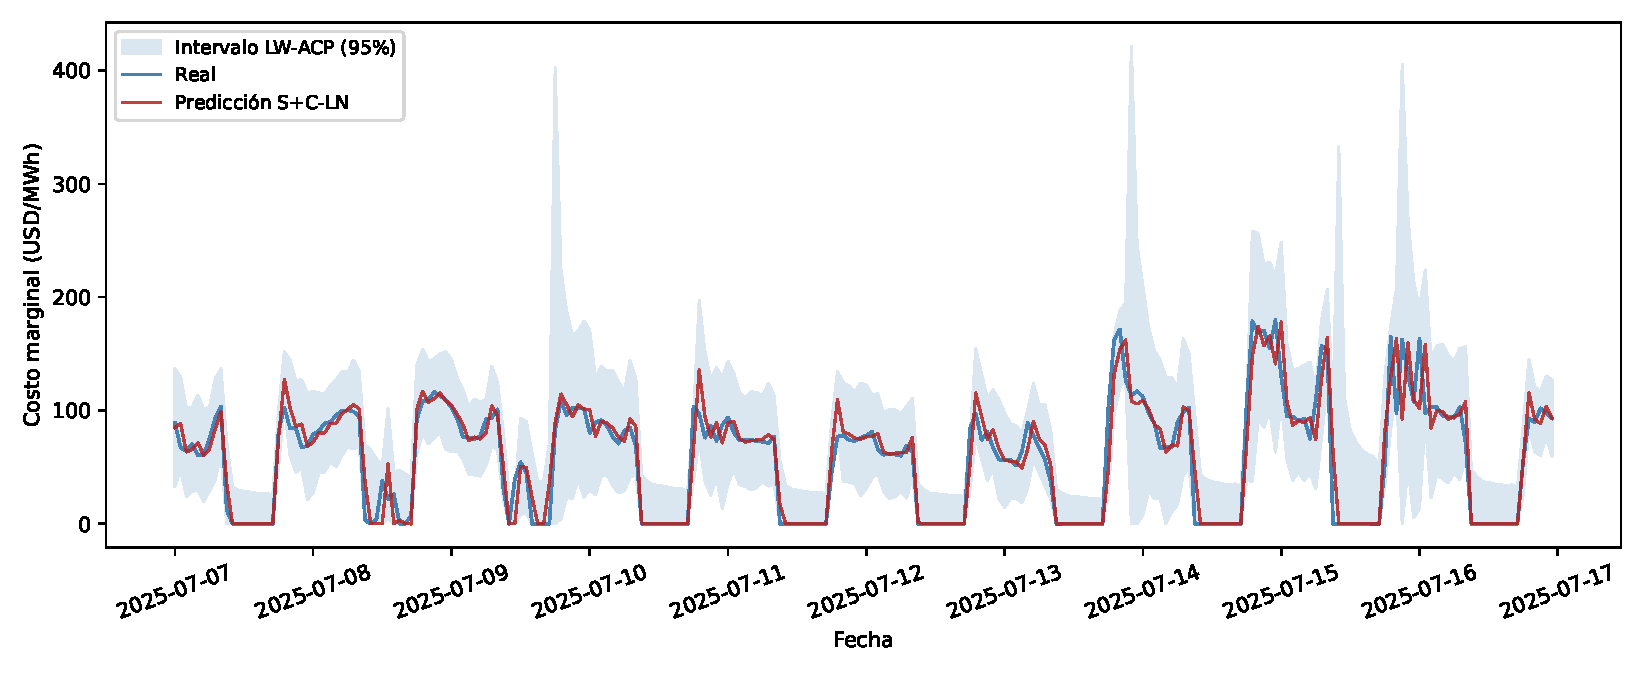
\includegraphics[width=0.75\textwidth]{imagenes/fig_cp_ejemplo_intervalo.pdf}
    \caption{Ejemplo de intervalo de predicción LW-ACP (95\% nominal) para Atacama, 12 de febrero de 2026. El intervalo se angosta en las horas de precio cero (mediodía, sobreoferta solar) y se ensancha en las horas de transición, capturando correctamente el \textit{peak} matutino sin dejar de ser informativo.}
    \label{fig:cp_ejemplo_intervalo}
\end{figure}

\subsection{Split CP clásico}
\label{sec:split_cp_clasico}

Consistente con la selección de S+C-LN como modelo de referencia para el resto de este capítulo (Sección \ref{sec:pc_vs_sc}), el Split CP clásico se construye directamente sobre la predicción cruda del $\text{TFT}_\text{LN}$ S+C, sin pasar por Stacking Optimization: no existe una combinación de múltiples predicciones con pesos aprendidos, por lo que no hay una columna de ``estrategia'' que varíe entre barras. Los resultados se presentan en la Tabla \ref{tab:scp_resultados}.

\begin{table}[htbp]
    \centering
    \small
    \begin{tabular}{lrrrr}
        \toprule
        Barra & Coverage & Width & MAE & $q$ \\
        \midrule
        Atacama       & 0.9648 & 54.68  & 6.70  & 34.07 \\
        Cardones      & 0.9595 & 53.58  & 6.63  & 33.25 \\
        Charrúa       & 0.9512 & 61.23  & 7.98  & 35.51 \\
        Crucero       & 0.9614 & 52.82  & 6.74  & 32.90 \\
        Pan de Azúcar & 0.9588 & 57.16  & 6.93  & 35.38 \\
        Puerto Montt  & 0.9600 & 110.41 & 13.68 & 64.05 \\
        Quillota      & 0.9530 & 64.25  & 8.26  & 37.43 \\
        Tarapacá      & 0.9623 & 56.23  & 7.11  & 35.24 \\
        \bottomrule
    \end{tabular}
    \caption{Resultados del Split CP clásico sobre S+C-LN, las ocho barras del SEN. Coverage nominal: 0.95. Width, MAE y $q$ en USD/MWh. El límite inferior de todos los intervalos se trunca en 0 USD/MWh, respetando el dominio físico del costo marginal; $q$ es el semiancho antes de truncar.}
    \label{tab:scp_resultados}
\end{table}

Los resultados muestran cobertura empírica por encima del nominal en las ocho barras. La cobertura oscila entre 0.9512 (Charrúa) y 0.9648 (Atacama), con anchos medios entre 52.8 (Crucero) y 64.3 USD/MWh (Quillota) en las siete barras del norte y centro, y un ancho considerablemente mayor en Puerto Montt (110.4 USD/MWh), consistente con su mayor dispersión de precio ya documentada en la Sección \ref{sec:pmontt_desempeno}. El caso de Charrúa es especialmente relevante: es la barra que más se acerca al nominal exacto, con una diferencia de cobertura de apenas 0.12 puntos porcentuales, consistente con que Charrúa es también la barra donde el TFT S+C tiene mayor MAE relativo entre las siete barras del norte y centro, lo que produce errores de calibración más representativos del comportamiento en prueba.

El ancho reportado en esta y las siguientes tablas de esta sección ya incorpora el truncamiento en 0 del límite inferior del intervalo, aplicado de manera uniforme a los cinco métodos (Split CP, ACI, LW Split CP, LW-ACP y CQR): dado que el costo marginal no toma valores negativos, un límite inferior negativo no aporta información y solo infla artificialmente el ancho reportado, sobre todo en horas de precio cercano a cero. El truncamiento no afecta la cobertura empírica --un intervalo $[\hat{y}-q, \hat{y}+q]$ con $\hat y - q<0$ cubre $y\geq 0$ exactamente cuando $[\max(\hat y-q,0), \hat y+q]$ también lo cubre--, por lo que las cifras de cobertura de esta sección son idénticas con o sin truncar; el efecto es puramente una reducción del ancho medio, más marcada cuanto más frecuentes son las horas de precio bajo en la barra.

La sobrecobertura observada en Atacama, de hasta 1.5 puntos porcentuales sobre el nominal, es el efecto esperado de un cuantil fijo calculado sobre el período de validación: si la distribución de errores en prueba es más concentrada que en calibración, el intervalo resulta conservadoramente ancho. Esta limitación motiva las variantes adaptativas.

Como se detalla en la Sección \ref{sec:cp_configuracion_general} del Marco Metodológico, la calibración de los cinco métodos de esta sección excluye una ventana de 11 horas de precio de falla administrativo (25--26 de febrero de 2025), verificada por el mismo valor exacto simultáneo en las ocho barras. Esta ventana cae en el conjunto de validación (calibración), no en prueba, por lo que no afecta directamente el MAE de prueba reportado en el resto de este capítulo, pero sí inflaba el cuantil de no conformidad antes de excluirla.

\subsection{ACI}
\label{sec:aci}

A diferencia de una formulación anterior de este trabajo, que construía un meta-modelo Ridge auxiliar (predicción de S+C-LN más las variables solares \texttt{elevacion\_solar} y \texttt{cos\_elevacion}) como predictor puntual para ACI, aquí ACI se evalúa sobre la misma predicción cruda de S+C-LN que Split CP, LW Split CP y LW-ACP: usar un predictor distinto por método impediría comparar el ancho de intervalo entre ellos de forma válida (Sección \ref{sec:lwacp_comparativa}), ya que el efecto del mecanismo de calibración quedaría mezclado con el efecto de cambiar el modelo base. Al no requerir ningún meta-modelo, ACI tampoco distingue entre una variante \textit{offline} y una \textit{online} --la distinción original aludía a si el meta-modelo se reajustaba en cada paso de prueba, algo que ya no aplica-- por lo que se reporta un único método. Se fija $\gamma = 0.05$ de antemano, el mismo valor usado en LW-ACP (Sección \ref{sec:lwacp_resultados}), en lugar de comparar varios valores de $\gamma$ y reportar el de mejor desempeño en prueba. Los resultados se presentan en la Tabla \ref{tab:aci_ln_resultados}.

\begin{table}[htbp]
    \centering
    \small
    \begin{tabular}{lrrrr}
        \toprule
        Barra & Coverage & Width & MAE & $\bar{\alpha}_t$ \\
        \midrule
        Atacama       & 0.9467 & 49.72  & 6.70  & 0.0878 \\
        Cardones      & 0.9465 & 47.14  & 6.63  & 0.0903 \\
        Charrúa       & 0.9443 & 57.14  & 7.98  & 0.0825 \\
        Crucero       & 0.9469 & 49.58  & 6.74  & 0.0890 \\
        Pan de Azúcar & 0.9461 & 49.32  & 6.93  & 0.0905 \\
        Puerto Montt  & 0.9471 & 105.71 & 13.68 & 0.0841 \\
        Quillota      & 0.9446 & 58.09  & 8.26  & 0.0818 \\
        Tarapacá      & 0.9472 & 52.88  & 7.11  & 0.0876 \\
        \bottomrule
    \end{tabular}
    \caption{Resultados de ACI sobre S+C-LN (predictor puntual crudo, sin meta-modelo) con $\gamma = 0.05$ fijo, las ocho barras del SEN. Coverage nominal: 0.95. Width y MAE en USD/MWh. $\bar{\alpha}_t$: media temporal del nivel adaptado.}
    \label{tab:aci_ln_resultados}
\end{table}

Dos patrones emergen de los resultados. Primero, la cobertura empírica se mantiene cercana al nominal en las ocho barras, con errores de cobertura entre 0.28 (Tarapacá) y 0.57 puntos porcentuales (Charrúa) --sensiblemente mejor que la sobrecobertura de 0.9--1.5 puntos de Split CP (Sección \ref{sec:split_cp_clasico})--, confirmando que la adaptación \textit{online} de $\alpha_t$ corrige el sesgo de sobrecobertura estructural del cuantil fijo. Segundo, y a diferencia de una lectura anterior de este mismo análisis --hecha antes de excluir de la calibración la ventana de precio de falla administrativo (Sección \ref{sec:split_cp_clasico})--, el ancho de intervalo de ACI \textbf{sí es sistemáticamente menor} que el de Split CP una vez que ambos comparten el mismo predictor puntual: el ancho promedio de ACI (58.7\,USD/MWh) es 8.0\% menor que el de Split CP (63.8), con una reducción que va de 4.3\% (Puerto Montt) a 13.7\% (Pan de Azúcar). El cuantil de no conformidad de un método de cuantil fijo como Split CP es especialmente sensible a un puñado de \textit{scores} de calibración inflados por un evento no representativo del mercado; la adaptación \textit{online} de $\alpha_t$, al recalcularse en cada paso de prueba en vez de fijarse una sola vez, resulta menos expuesta a ese mismo sesgo. El aporte de ACI, medido correctamente, es entonces doble: mejor calibración y un intervalo más angosto, no solo lo primero.

\subsection{LW Split CP}
\label{sec:lw_split_cp}

Al igual que Split CP clásico y ACI (Secciones \ref{sec:split_cp_clasico}--\ref{sec:aci}), LW Split CP y LW-ACP (Sección \ref{sec:lwacp_resultados}) se evalúan sobre S+C-LN, manteniendo la misma arquitectura, rama y predictor puntual en las ocho barras. La Tabla \ref{tab:lwscp_resultados} presenta los resultados de LW Split CP.

\begin{table}[htbp]
    \centering
    \small
    \begin{tabular}{lrrr}
        \toprule
        Barra & Coverage & Width & MAE \\
        \midrule
        Atacama       & 0.9651 & 55.80  & 6.70  \\
        Cardones      & 0.9588 & 54.19  & 6.63  \\
        Charrúa       & 0.9537 & 61.79  & 7.98  \\
        Crucero       & 0.9623 & 53.76  & 6.74  \\
        Pan de Azúcar & 0.9601 & 56.75  & 6.93  \\
        Puerto Montt  & 0.9597 & 109.53 & 13.68 \\
        Quillota      & 0.9535 & 62.98  & 8.26  \\
        Tarapacá      & 0.9612 & 56.67  & 7.11  \\
        \bottomrule
    \end{tabular}
    \caption{Resultados de LW Split CP sobre S+C-LN, las ocho barras del SEN. Coverage nominal: 0.95. Width y MAE en USD/MWh.}
    \label{tab:lwscp_resultados}
\end{table}

La cobertura empírica se mantiene por encima del nominal en las ocho barras, entre 0.9535 (Quillota) y 0.9651 (Atacama), un patrón de sobrecobertura similar al de Split CP clásico (Sección \ref{sec:split_cp_clasico}) y esperable dado que LW Split CP hereda el mismo mecanismo de cuantil fijo, solo que aplicado sobre \textit{scores} normalizados por hora. El ancho medio, sin embargo, \textbf{no se reduce de forma consistente} respecto a Split CP clásico: sube en Atacama (+2.1\%), Cardones (+1.1\%), Charrúa (+0.9\%), Crucero (+1.8\%) y Tarapacá (+0.8\%), y baja levemente en Pan de Azúcar (-0.7\%), Puerto Montt (-0.8\%) y Quillota (-2.0\%), sin una dirección predominante (63.9 vs.\ 63.8\,USD/MWh en promedio sobre las ocho barras, +0.2\%). Esto contrasta con ACI (Sección \ref{sec:aci}), que sí reduce el ancho de forma sistemática y por un margen considerable (8.0\%): la ponderación local por hora, aplicada sola y sin la adaptación \textit{online} de $\alpha_t$, no es suficiente para capturar una ganancia de eficiencia -- la Sección \ref{sec:lwacp_comparativa} retoma esta comparación con los cinco métodos en conjunto.

\subsection{LW-ACP Online}
\label{sec:lwacp_resultados}

La Tabla \ref{tab:lwacp_resultados} presenta los resultados de LW-ACP sobre S+C-LN, la variante que combina la ponderación local por hora con la actualización online del nivel de cobertura de ACI (Sección \ref{sec:lwacp}), con $\gamma = 0.05$ fijo, el mismo valor usado en ACI (Sección \ref{sec:aci}) y no seleccionado comparando contra el resultado en prueba.

\begin{table}[htbp]
    \centering
    \small
    \begin{tabular}{lrrr}
        \toprule
        Barra & Coverage & Width & MAE \\
        \midrule
        Atacama       & 0.9471 & 49.62  & 6.70  \\
        Cardones      & 0.9461 & 48.47  & 6.63  \\
        Charrúa       & 0.9440 & 56.29  & 7.98  \\
        Crucero       & 0.9471 & 49.99  & 6.74  \\
        Pan de Azúcar & 0.9461 & 48.96  & 6.93  \\
        Puerto Montt  & 0.9475 & 101.34 & 13.68 \\
        Quillota      & 0.9440 & 58.04  & 8.26  \\
        Tarapacá      & 0.9476 & 53.33  & 7.11  \\
        \bottomrule
    \end{tabular}
    \caption{Resultados de LW-ACP ($\gamma = 0.05$) sobre S+C-LN, las ocho barras del SEN. Coverage nominal: 0.95. Width y MAE en USD/MWh.}
    \label{tab:lwacp_resultados}
\end{table}

La cobertura empírica de LW-ACP se mantiene cerca del nominal: las ocho barras caen en el rango $[0.9440,\, 0.9476]$, es decir, entre 0.24 y 0.60 puntos porcentuales del nominal 0.95, más ajustado que la sobrecobertura de 0.1--1.5 puntos porcentuales observada en Split CP clásico y LW Split CP, aunque sin la precisión casi exacta que se obtenía con $\gamma = 0.01$ --el valor con el que se había barrido inicialmente, y que producía una desviación media de solo 0.02 puntos porcentuales, pero que no puede adoptarse sin verse influido por su desempeño en prueba (Sección \ref{sec:lwacp_comparativa})--. Esto confirma que el mecanismo de adaptación online de $\alpha_t$, heredado de ACI, corrige de manera efectiva el sesgo de sobrecobertura estructural de los métodos de cuantil fijo, sin necesidad de reentrenar ningún modelo, aunque la magnitud exacta de esa corrección depende de $\gamma$.

Al mismo tiempo, LW-ACP produce los intervalos más angostos de los cinco métodos evaluados, incluyendo CQR como comparación externa (Sección \ref{sec:lwacp_comparativa}): una reducción promedio de 8.7\% respecto a Split CP clásico, con el mayor beneficio en Pan de Azúcar (14.4\%) y Cardones (9.5\%), y el menor en Tarapacá (5.2\%) y Crucero (5.4\%). La mayor parte de esta reducción ya está presente en ACI solo (8.0\% respecto a Split CP, Sección \ref{sec:aci}); la ponderación local por hora, agregada sobre la adaptación \textit{online}, aporta una reducción adicional modesta (LW-ACP es 0.8\% más angosto que ACI en promedio) pero no uniforme, angosto en cinco de las ocho barras y levemente más ancho en las otras tres (Cardones, Crucero, Tarapacá). La combinación de una cobertura cercana al nominal y el ancho más angosto de los cinco métodos muestra que, con un $\gamma$ fijado de antemano y no elegido por su resultado en prueba, LW-ACP explota dos fuentes de información distintas --la heterocedasticidad horaria conocida de antemano, vía $\hat{\sigma}_h$, y el error de cobertura reciente, vía $\alpha_t$--, aunque la segunda explica la mayor parte de la ganancia y la primera aporta un refinamiento adicional, no una fuente de eficiencia comparable por sí sola (Sección \ref{sec:lw_split_cp}).

\subsection{Comparativa de métodos: SCP, ACP, LW-ACP y CQR}
\label{sec:lwacp_comparativa}

Con todos los métodos evaluados sobre S+C-LN y sobre el mismo predictor puntual crudo, las tres variantes principales de Split CP forman un linaje conceptual de dos pasos, más una comparación externa: Split CP (SCP) es el método base de calibración por cuantil fijo (Sección \ref{sec:split_cp_clasico}); ACP añade adaptación \textit{online} del nivel de cobertura, el mecanismo de Gibbs y Candès (2021, Sección 2.6.4), correspondiente a ACI con $\gamma = 0.05$ (Sección \ref{sec:aci}); y LW-ACP, la contribución de este trabajo, añade además ponderación local por hora (Sección \ref{sec:lwacp_resultados}, Sección \ref{sec:lwacp} del Marco Teórico). CQR se incluye como comparación externa a la familia de Conformal Prediction (Sección 2.6.2), al estimar cuantiles condicionales directamente mediante regresión cuantílica en vez de calibrar un cuantil de no conformidad. La Tabla \ref{tab:lw_comparativa} resume el ancho medio, la desviación de cobertura y el \textit{interval score} de Winkler --que penaliza conjuntamente el ancho del intervalo y la magnitud de la no-cobertura, a diferencia del ancho y la cobertura marginal por separado (Sección \ref{sec:metricas_cp})-- de los cuatro métodos, promediados sobre las ocho barras.

\begin{table}[htbp]
    \centering
    \begin{tabular}{lrrr}
        \toprule
        Método & Width medio (USD/MWh) & $|$Coverage $-$ 0.95$|$ medio & Winkler medio \\
        \midrule
        Split CP (SCP)              & 63.80 & 0.0089 & 100.78 \\
        ACP (ACI, $\gamma=0.05$)    & 58.70 & 0.0038 & 90.64 \\
        LW-ACP ($\gamma=0.05$)      & \textbf{58.25} & \textbf{0.0038} & \textbf{89.89} \\
        CQR                         & 67.99 & 0.0081 & 96.50 \\
        \bottomrule
    \end{tabular}
    \caption{Comparación del linaje SCP $\to$ ACP $\to$ LW-ACP, más CQR como comparación externa, evaluados sobre S+C-LN con el mismo predictor puntual crudo (ocho barras). Width y Winkler promedio en USD/MWh; desviación absoluta media respecto a la cobertura nominal 0.95.}
    \label{tab:lw_comparativa}
\end{table}

El linaje SCP $\to$ ACP $\to$ LW-ACP, con $\gamma = 0.05$ fijado de antemano y el mismo predictor puntual crudo en los tres métodos, muestra que casi toda la ganancia del linaje proviene de un solo mecanismo. ACP, que solo añade adaptación \textit{online} del nivel de cobertura, sin ponderación horaria ni cambio de predictor, reduce la desviación de cobertura en 57\% (de 0.0089 a 0.0038 puntos) respecto a SCP, y \textbf{también reduce el ancho medio} de forma sustancial: con 58.70\,USD/MWh resulta 8.0\% más angosto que SCP (Sección \ref{sec:aci}). LW-ACP, que agrega la ponderación por hora sobre ese mismo mecanismo \textit{online}, reduce el ancho un poco más, hasta 58.25\,USD/MWh (8.7\% respecto a SCP), con una calibración prácticamente idéntica a la de ACP solo (0.0038 en ambos). En conjunto, esto acota con precisión qué aporta cada mecanismo, y corrige una lectura anterior de este mismo análisis: la adaptación \textit{online} de $\alpha_t$ por sí sola ya explica la gran mayoría de la mejora, tanto en calibración como en ancho; la ponderación horaria por sí sola, sin adaptación \textit{online}, no aporta una reducción de ancho consistente (Sección \ref{sec:lw_split_cp}), y solo aporta un refinamiento adicional modesto cuando se combina con la adaptación \textit{online} en LW-ACP. CQR, evaluado de forma independiente de la familia CP, resulta en este caso el \textbf{más ancho} de los cuatro métodos (67.99\,USD/MWh) y con peor calibración que ACP y LW-ACP (0.0081 de desviación, más del doble): a diferencia de los tres métodos conformes, cuyo intervalo se trunca en 0 de forma directa sobre un semiancho ya angosto, los cuantiles de CQR se estiman por regresión cuantílica condicional y ya incorporan una asimetría propia que deja menos margen para que el truncamiento en 0 reduzca su ancho reportado. El \textit{interval score} de Winkler, que combina ambas dimensiones en una sola métrica, confirma este orden (LW-ACP $<$ ACP $<$ CQR $<$ SCP): LW-ACP obtiene el mejor puntaje (89.89), seguido de cerca por ACP (90.64), con CQR intermedio (96.50) y SCP claramente peor (100.78, 12\% más alto que LW-ACP). LW-ACP es entonces el único de los cuatro métodos que combina el mejor resultado en las tres métricas --ancho, calibración y Winkler-- de forma simultánea.

Queda fuera de esta comparación agregada, aunque se presenta en su propia sección, LW Split CP (Sección \ref{sec:lw_split_cp}), que pondera por hora sin adaptación \textit{online}: confirma, desde la dirección opuesta a ACP, que la ponderación horaria por sí sola no es la fuente principal de la eficiencia observada en LW-ACP.

\subsection{Cobertura condicional por hora y por mes}
\label{sec:cobertura_condicional}

La cobertura marginal cercana al nominal reportada hasta aquí es un promedio sobre todo el conjunto de prueba, y puede ocultar heterogeneidad sistemática si el método sub-cubre en algunas horas o meses y sobre-cubre en otras, compensándose en el promedio. Esta sección desagrega la cobertura de Split CP, ACP y LW-ACP --el linaje completo (Sección \ref{sec:lwacp_comparativa})-- por hora del día y por mes, promediando sobre las ocho barras.

La Figura \ref{fig:cp_cobertura_ancho_hora} presenta la cobertura y el ancho medio por hora del día para los tres métodos. Incluir a ACP, no solo los dos extremos del linaje, permite distinguir si la caída de cobertura en horas de transición es un efecto de la adaptación \textit{online} en sí, o específico de agregarle la ponderación horaria: la Figura \ref{fig:cp_cobertura_ancho_hora} muestra que ACP y LW-ACP caen de forma casi idéntica en esas horas (0.902 vs.\ 0.898), mientras que Split CP, sin adaptación \textit{online}, cae menos (0.943). La caída es entonces atribuible al mecanismo de adaptación \textit{online} de $\alpha_t$, compartido por ambos métodos, no a la ponderación horaria que solo LW-ACP incorpora.

\begin{figure}[htbp]
    \centering
    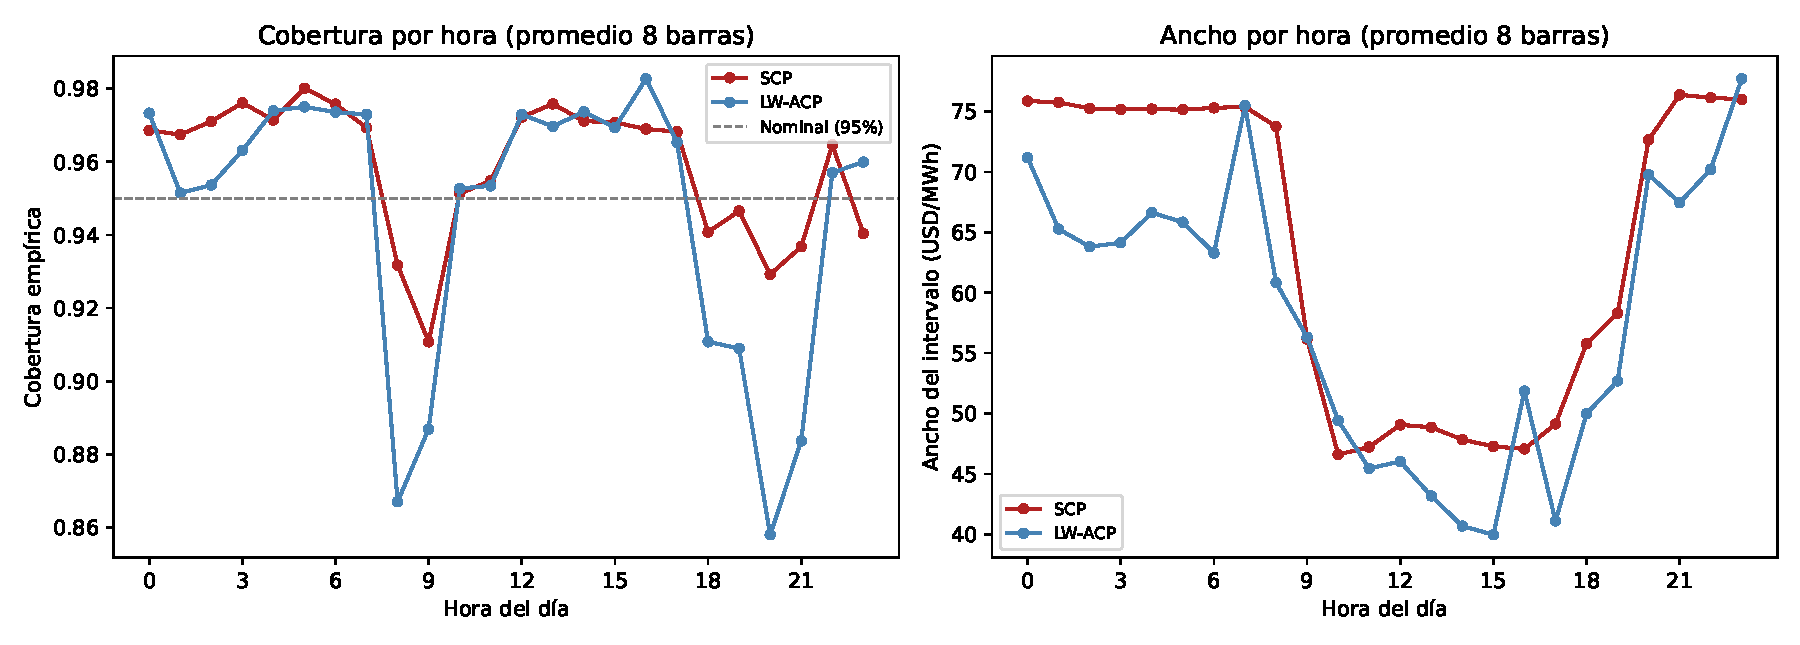
\includegraphics[width=\textwidth]{imagenes/fig_cp_cobertura_ancho_hora.pdf}
    \caption{Cobertura empírica (izquierda) y ancho medio del intervalo (derecha) por hora del día, Split CP vs.\ ACP vs.\ LW-ACP, promediado sobre las ocho barras. ACP y LW-ACP son más angostos que Split CP casi todo el día, pero ambos --no solo LW-ACP-- caen marcadamente por debajo del nominal en las horas de transición solar (7--9h, 19--21h).}
    \label{fig:cp_cobertura_ancho_hora}
\end{figure}

Por mes, LW-ACP es marcadamente más estable que Split CP: la desviación estándar de la cobertura mensual es 0.0048 para LW-ACP frente a 0.0280 para Split CP, casi seis veces menor. Split CP oscila entre 0.899 (junio) y 0.991 (marzo), mientras que las doce cifras mensuales de LW-ACP caen todas en el rango estrecho $[0.933,\, 0.950]$. Esta es precisamente la ventaja esperada de la adaptación \textit{online} de $\alpha_t$: al reaccionar al historial reciente de cobertura, LW-ACP corrige la deriva estacional que un cuantil fijo como el de Split CP no puede seguir.

Por hora del día, sin embargo, el resultado es el opuesto: la desviación estándar de la cobertura horaria es 0.0181 para Split CP frente a 0.0370 para LW-ACP, más del doble. La brecha se concentra exactamente en las horas de transición solar (7, 8, 19, 20 y 21h) que el análisis de errores extremos (Sección \ref{sec:errores_extremos}) ya identifica como el origen del desfase de fase: ahí la cobertura promedio de LW-ACP cae a 0.898, 5.2 puntos porcentuales bajo el nominal y 4.5 puntos por debajo de Split CP (0.943) en esas mismas horas, mientras que en el resto de las horas ambos métodos son similares (0.959 LW-ACP vs.\ 0.963 Split CP). Es decir, la ponderación horaria por sí sola no logra homogeneizar la cobertura entre horas --la motivación original de $\hat\sigma_h$--, y en las horas más difíciles del día, las mismas donde se concentra el desfase de fase, LW-ACP cubre peor que el cuantil fijo sin ponderar, no mejor.

Esto es coherente con el hallazgo de la Sección \ref{sec:lwacp_comparativa}: la eficiencia de LW-ACP proviene mayoritariamente de la adaptación \textit{online} de $\alpha_t$, un mecanismo que opera sobre la dimensión temporal mes a mes, no sobre la dimensión horaria intradía. $\hat\sigma_h$ ajusta el \textit{ancho} del intervalo según la variabilidad histórica de cada hora, pero no ajusta el \textit{nivel de cobertura} por hora --ese es un único $\alpha_t$ compartido por las 24 horas del día--, por lo que un error sistemático concentrado en horas específicas, como el desfase de fase, no se corrige de la misma forma en que la adaptación \textit{online} sí corrige la deriva estacional. Esta limitación motiva directamente la variante de $\alpha_t$ indexado por hora propuesta como trabajo futuro (Conclusiones).

\subsection{Selección del mejor método de CP}

LW-ACP es el método de Conformal Prediction seleccionado para el pipeline final. Es el único de los cuatro métodos que combina el mejor resultado en las tres métricas evaluadas: el ancho medio más angosto (58.25\,USD/MWh, 8.7\% menor que Split CP), la mejor calibración (0.0038 de desviación media, empatado con ACP y menos de la mitad de la desviación de CQR) y el mejor \textit{interval score} de Winkler (89.89, Sección \ref{sec:lwacp_comparativa}), dentro de 0.24--0.60 puntos porcentuales del nominal en las ocho barras (Sección \ref{sec:lwacp_resultados}). A diferencia de CQR, que no ofrece garantías de cobertura marginal finita sin supuestos distribucionales y que en esta comparación resulta ser el método más ancho de los cuatro, LW-ACP hereda la garantía de cobertura marginal asintótica de la familia conforme, y logra además reducir el ancho respecto a Split CP en las ocho barras sin excepción (Sección \ref{sec:lwacp_resultados}). Esta ventaja en ancho proviene principalmente de la adaptación \textit{online} del nivel de cobertura, heredada de ACP, con un aporte adicional --menor, y consistente en cinco de las ocho barras-- de la ponderación horaria vía $\hat{\sigma}_h$ (Sección \ref{sec:lwacp_comparativa}).

La cobertura condicional (Sección \ref{sec:cobertura_condicional}) matiza esta elección sin invalidarla: LW-ACP es notablemente más estable que Split CP mes a mes, pero menos uniforme hora a hora, con una brecha de cobertura concreta en las horas de transición solar donde se concentra el desfase de fase. La elección de LW-ACP se sostiene en su desempeño marginal --ancho, calibración y Winkler score-- y en su estabilidad temporal frente a la deriva estacional, no en haber resuelto la heterogeneidad horaria del error, que sigue siendo una limitación abierta.

Cabe señalar una limitación metodológica del diseño experimental: el conjunto de validación cumple simultáneamente el rol de selección del mejor ensamble y de calibración del CP, lo que introduce un sesgo optimista en el cuantil de no conformidad. Este sesgo es esperablemente pequeño dado el tamaño del conjunto de calibración ($n_{\text{cal}} = 8\,298$) y la estabilidad de los residuos del ensamble, pero se reporta para transparencia metodológica.

\subsection{Análisis de errores extremos}
\label{sec:errores_extremos}

La brecha entre el MAE promedio del modelo (6.89\,USD/MWh en validación para Atacama) y el semiancho de los intervalos de Split CP clásico ($q = 32.72$\,USD/MWh, Sección \ref{sec:split_cp_clasico}) sugiere que la distribución de errores del modelo no es simétrica ni de cola ligera. Para comprender el origen de esta brecha, se examina la distribución de errores absolutos en validación para las ocho barras, con Atacama como caso ilustrativo y el detalle completo del resto en el Anexo \ref{anexo:errores_extremos}.

La Figura \ref{fig:error_dist_atacama} muestra la distribución de
errores absolutos del $\text{TFT}_\text{LN}$ (S+C) en validación para Atacama. La distribución presenta una forma exponencial decreciente fuertemente concentrada: más del 90\% de las predicciones tienen un error menor a 19.8\,USD/MWh, y el percentil 95 es de 32.5\,USD/MWh. Sin embargo, la distribución exhibe una cola derecha extendida que alcanza los 162.9\,USD/MWh, marcada explícitamente en la figura. Es precisamente esta cola la que determina el cuantil de calibración del Split CP: $q = 32.72$\,USD/MWh corresponde aproximadamente al percentil 95 de la distribución de errores de validación, de modo que el ancho del intervalo queda dominado por el 5\% de los errores más grandes. Las ocho barras exhiben la misma forma general, con el máximo desplazándose entre 132.4 (Charrúa) y 241.7\,USD/MWh (Puerto Montt); ver Anexo \ref{anexo:errores_extremos} para el detalle de errores por barra.

\begin{figure}[htbp]
    \centering
    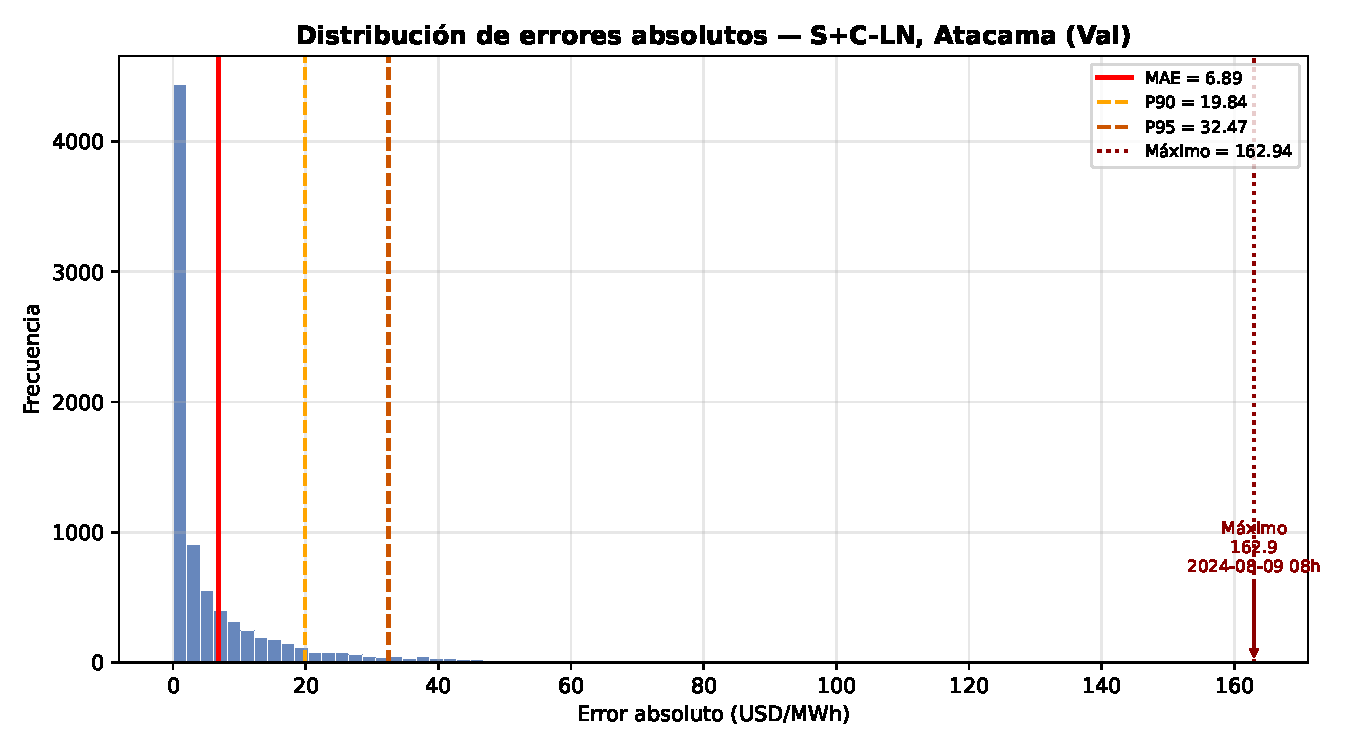
\includegraphics[width=0.95\textwidth]{imagenes/fig_error_dist_atacama.pdf}
    \caption{Distribución de errores absolutos del $\text{TFT}_\text{LN}$ (S+C)
    en el conjunto de validación para la barra Atacama ($n = 8\,298$ observaciones).  Las líneas verticales indican el MAE (rojo), el percentil 90 (naranja claro), el percentil 95 (naranja oscuro) y el error máximo (granate, punteado), este último señalado además con una flecha dado lo alejado que queda del grueso de la distribución.}
    \label{fig:error_dist_atacama}
\end{figure}

Una primera hipótesis ante una cola de este tipo es que los errores
extremos correspondan a eventos inusuales de la propia serie temporal: spikes de costo marginal asociados a indisponibilidades, eventos climáticos o cambios regulatorios que el modelo no puede anticipar por construcción, dado que no dispone de información futura sobre dichos eventos. Bajo esa hipótesis, los errores grandes serían inherentes a la naturaleza del problema y no reflejarían una deficiencia del modelo. Para evaluar esta hipótesis, se examinan en detalle los 20 errores absolutos más grandes del conjunto de validación de cada barra: se recalcula el error tras desplazar la predicción entre $-3$ y $+3$ horas respecto de su posición original, y se retiene el desplazamiento que minimiza el error resultante; si la reducción de error alcanzada supera el 60\%, el caso se clasifica como \textit{desfase de fase}, y como \textit{evento estructural} en caso contrario. El Anexo \ref{anexo:errores_extremos} presenta la tabla completa de los 20 mayores errores para cada barra; la Tabla \ref{tab:sintesis_errores} resume los resultados a nivel de todo el SEN.

\begin{table}[htbp]
    \centering
    \small
    \begin{tabular}{lrrrrr}
        \toprule
        Barra & MAE & P95 & Máximo & Desfase de fase & Transición solar \\
        \midrule
        Atacama       & 6.89  & 32.47 & 162.94 & 17/20 & 12/20 \\
        Cardones      & 6.91  & 32.15 & 164.48 & 17/20 & 11/20 \\
        Charrúa       & 7.78  & 35.18 & 132.36 & 17/20 &  9/20 \\
        Crucero       & 6.95  & 31.46 & 174.38 & 18/20 & 13/20 \\
        Pan de Azúcar & 7.41  & 35.07 & 143.70 & 17/20 & 10/20 \\
        Puerto Montt  & 14.97 & 63.83 & 241.73 & 20/20 &  1/20 \\
        Quillota      & 7.98  & 37.05 & 144.20 & 16/20 &  8/20 \\
        Tarapacá      & 7.36  & 33.21 & 169.64 & 17/20 & 15/20 \\
        \bottomrule
    \end{tabular}
    \vspace{0.2cm}
    \caption{Síntesis del análisis de errores extremos en validación, las ocho barras del SEN. MAE, P95 y Máximo en USD/MWh. \textit{Desfase de fase}: cuántos de los 20 mayores errores se clasifican como tal (vs.\ \textit{evento estructural}). \textit{Transición solar}: cuántos de los 20 ocurren en las horas 07:00--08:00 o 19:00--21:00. Detalle completo por barra en el Anexo \ref{anexo:errores_extremos}.}
    \label{tab:sintesis_errores}
\end{table}

El análisis cuantitativo descarta en gran medida la hipótesis de
eventos inusuales en la serie: en las ocho barras, entre el 80\% y el 100\% de los 20 mayores errores corresponden a un \textit{desfase de fase} y no a spikes anómalos del costo marginal, con una reducción de error mediana entre el 84\% y el 98\% al desplazar la predicción (típicamente 1 hora, ocasionalmente 2). El sentido del desplazamiento es sistemáticamente el mismo en las ocho barras: entre el 76\% y el 94\% de los casos de desfase requieren un desplazamiento positivo, es decir, \textbf{el modelo predice la transición del costo marginal con un retraso aproximado de una hora respecto a la transición real}, un patrón consistente en todo el SEN y no un artefacto de una barra particular.

Puerto Montt es la excepción que confirma la regla: sus 20 mayores errores se clasifican \emph{todos} como desfase de fase (reducción mediana del 98\%, la más alta del grupo), pero solo 1 de 20 ocurre en las horas de transición solar 07:00--08:00 o 19:00--21:00, frente a 8--15 de 20 en las siete barras restantes. Esto es consistente con el resto de la caracterización de Puerto Montt en este capítulo (Sección \ref{sec:pmontt_desempeno}): el desfase de fase es un patrón general del modelo, no específico del ciclo solar, y en Puerto Montt se manifiesta alrededor de la dinámica hidrológica de la zona en vez de las transiciones de amanecer/atardecer.

La Figura \ref{fig:phase_shift_panel} ilustra cuatro casos
representativos de Atacama: tres desfases de fase en transiciones de amanecer o atardecer, y un evento estructural, un spike abrupto en la serie real que el modelo suaviza, consistente con un evento de indisponibilidad o redespacho no capturado por las covariables disponibles. Los paneles equivalentes para las siete barras restantes se presentan en el Anexo \ref{anexo:errores_extremos}.

\begin{figure}[htbp]
    \centering
    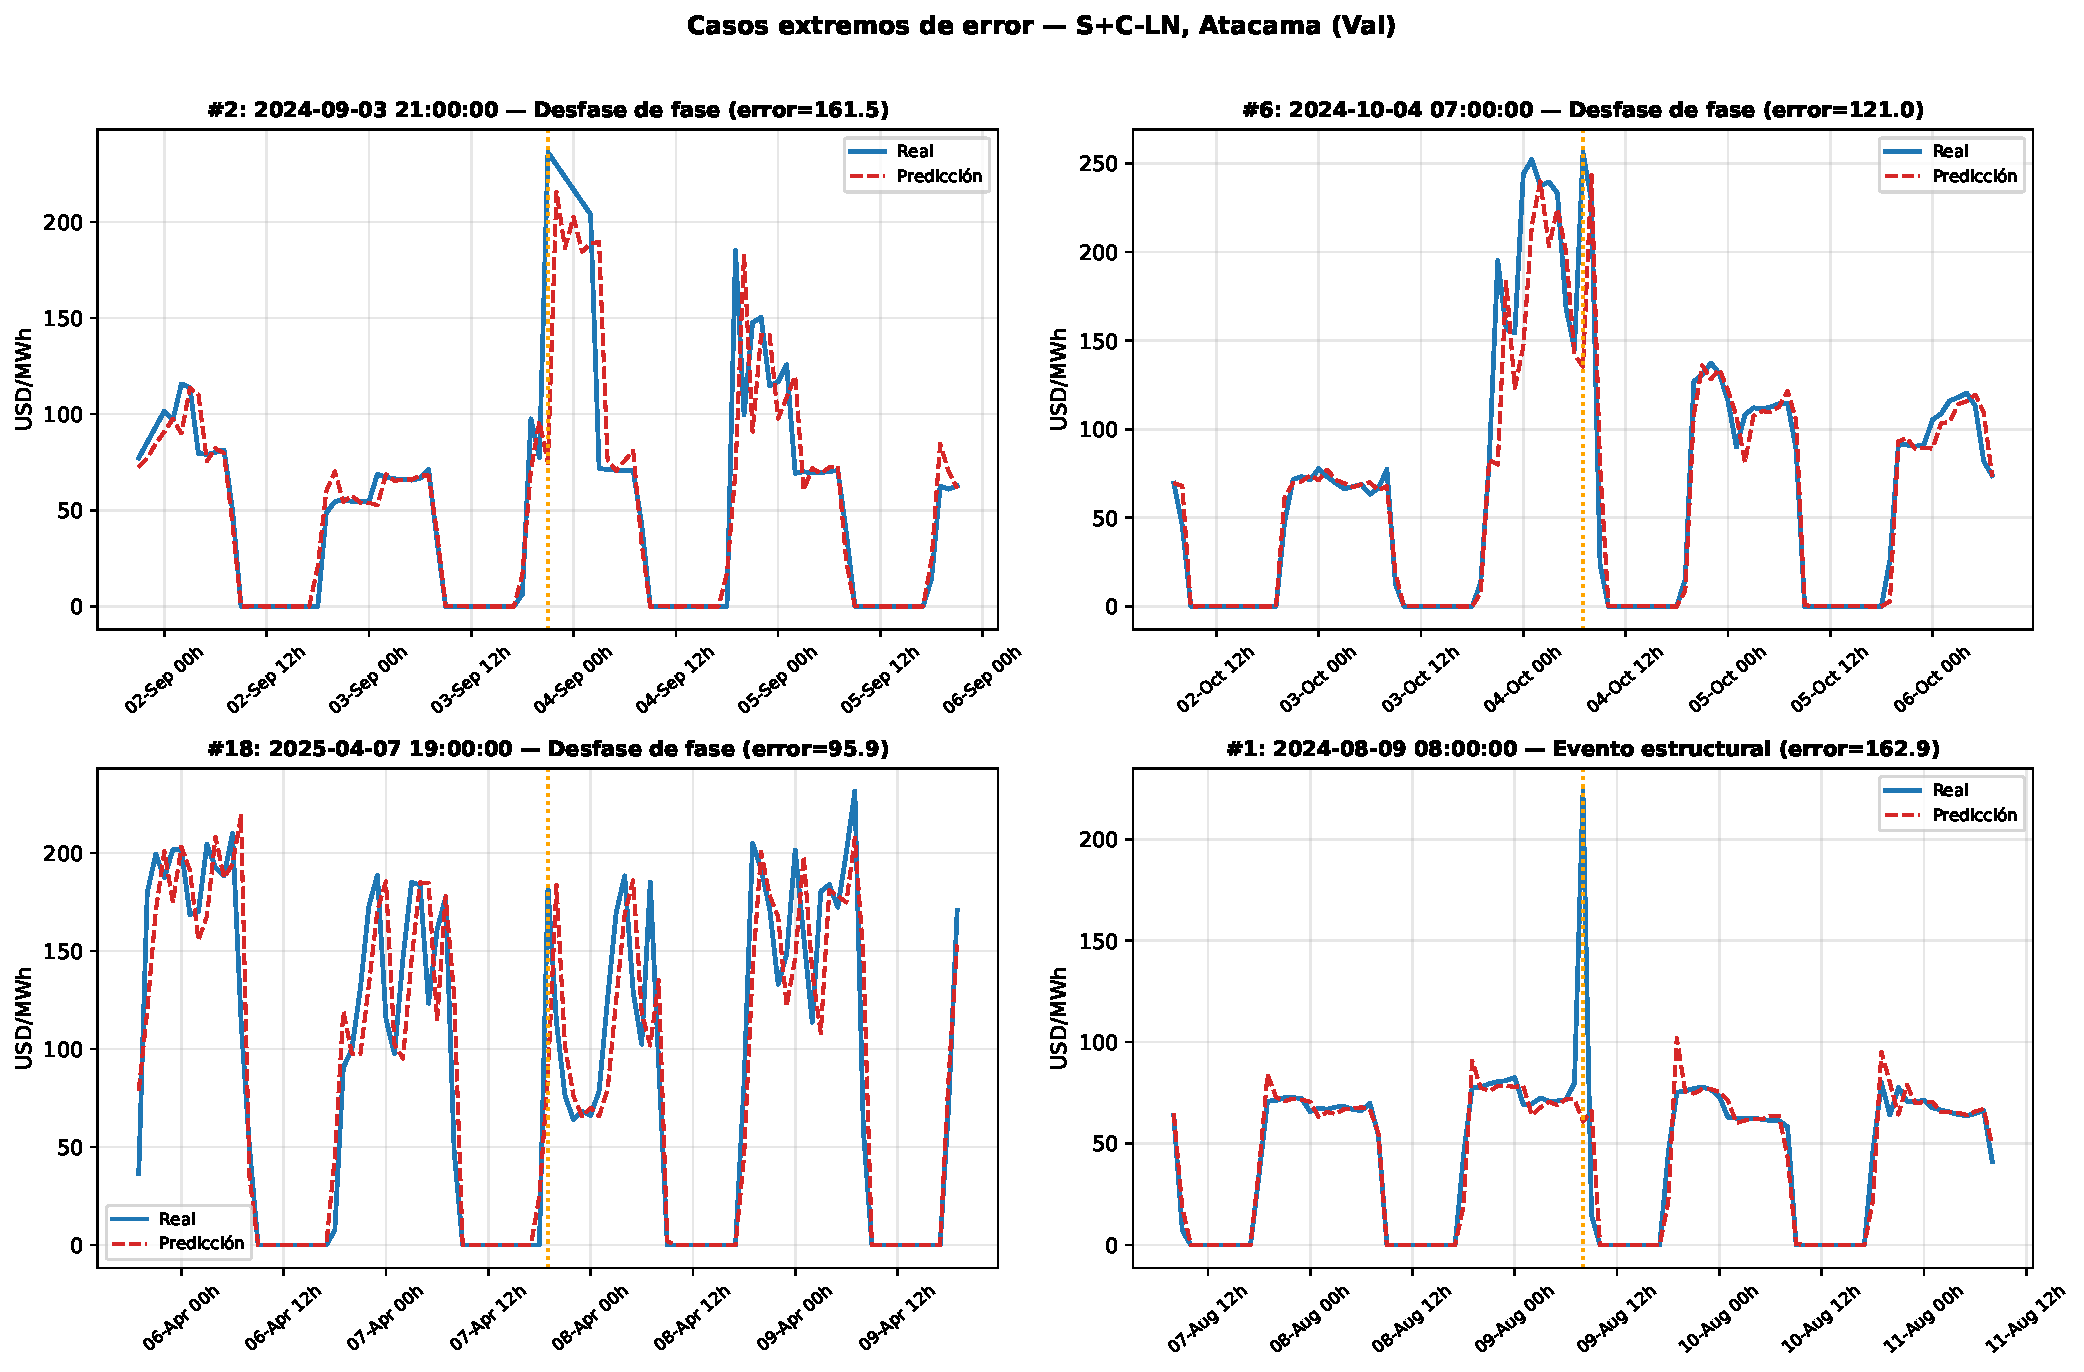
\includegraphics[width=\textwidth]{imagenes/fig_phase_shift_panel_2x2.pdf}
    \caption{Casos extremos de error del $\text{TFT}_\text{LN}$ (S+C) para
    la barra Atacama en validación.  Cada panel muestra una ventana de
    $\pm$48\,h alrededor del instante de error máximo (línea vertical
    punteada naranja).  La curva azul corresponde al CMg real y la
    curva roja punteada a la predicción.}
    \label{fig:phase_shift_panel}
\end{figure}

Esta caracterización tiene una implicancia directa para la
Conformal Prediction: los errores de desfase de fase son, por
construcción, de gran amplitud instantánea pero muy localizados en el
tiempo.  Un cuantil de calibración calculado sobre el percentil 95 de
todos los errores de validación necesariamente incorpora estos eventos
extremos, resultando en anchos de intervalo que sobreestiman
la incertidumbre en el $\sim$95\% restante de las horas donde el modelo
opera sin desfase.  Esta es la causa fundamental de la brecha entre el
MAE y el semiancho del intervalo observada en las ocho barras
(Tabla \ref{tab:scp_resultados}): ambas métricas son estadísticamente correctas, pero
describen regímenes distintos de la misma distribución de errores. Esta
brecha estructural, presente de forma consistente en todo el SEN, es a su vez la motivación central de las variantes
adaptativas de CP presentadas en las secciones anteriores.

\section{Análisis de interpretabilidad del TFT}
 
Una ventaja distintiva del TFT respecto a otros modelos de aprendizaje profundo es que su arquitectura produce medidas de importancia de variables de manera nativa a través de la Variable Selection Network (VSN) descrita en la Sección 2.3.4. Esta sección analiza la importancia relativa de cada \textit{feature} en el encoder y el decoder de S+C-LN, la estrategia adoptada como referencia (Sección \ref{sec:pc_vs_sc}), para las ocho barras del SEN, con el objetivo de verificar si el TFT efectivamente aprende a apoyarse en la posición solar. La importancia se reporta como el porcentaje del peso total asignado por la VSN a cada variable, promediado sobre todas las muestras del conjunto de prueba.
 
\subsection{Importancia de variables}
\label{sec:interpretabilidad_sc}

Esta subsección examina si el TFT efectivamente aprende a apoyarse en la posición solar, mediante el análisis de importancia de variables de S+C-LN. El encoder recibe la serie de precios, las cinco variables climáticas y las tres variables de posición solar (\texttt{elevacion\_solar}, \texttt{cos\_elevacion}, \texttt{es\_horario\_verano}); el decoder recibe únicamente estas tres variables solares más el índice temporal relativo, al no incluir S+C componentes de Prophet ni de residuo.

La Tabla \ref{tab:importancia_sc_encoder} presenta la importancia en el encoder, agregada en cuatro categorías para facilitar la comparación entre barras.

\begin{table}[htbp]
    \centering
    \small
    \begin{tabular}{lrrrr}
        \toprule
        Barra & \texttt{y\_real} & Posición solar & Clima & \texttt{relative\_time\_idx} \\
        \midrule
        Atacama       & 66.50 & 17.16 & 13.48 & 2.87 \\
        Cardones      & 70.88 & 16.08 & 10.47 & 2.58 \\
        Charrúa       & 54.52 & 21.98 & 14.21 & 9.29 \\
        Crucero       & 62.18 & 20.81 & 12.77 & 4.25 \\
        Pan de Azúcar & 58.17 & 17.86 & 19.77 & 4.20 \\
        Puerto Montt  & 84.09 &  9.00 &  5.16 & 1.76 \\
        Quillota      & 59.64 & 25.14 & 14.15 & 1.06 \\
        Tarapacá      & 72.07 & 14.42 & 10.89 & 2.63 \\
        \bottomrule
    \end{tabular}
    \vspace{0.2cm}
    \caption{Importancia agregada en el encoder de S+C ($\text{TFT}_\text{LN}$), por barra. ``Posición solar'' agrupa \texttt{elevacion\_solar}, \texttt{cos\_elevacion} y \texttt{es\_horario\_verano}; ``Clima'' agrupa las cinco variables climáticas. Porcentajes sobre el total del encoder.}
    \label{tab:importancia_sc_encoder}
\end{table}

\texttt{y\_real} domina el encoder de forma universal (54.5\%--84.1\%), y Puerto Montt es el caso extremo, con la mayor concentración en la serie propia (84.1\%) y, en este caso, también el menor peso conjunto de posición solar (9.0\%) y clima (5.2\%) de las ocho barras, consistente con que Puerto Montt es también la barra con menor mejora al agregar features exógenas en el estudio de ablación (Sección 4.7.3, mejora de apenas 2.9\%) y con menor ventaja estadística de LN sobre DyT (Sección \ref{sec:ln_vs_dyt}). En las siete barras restantes, la posición solar recibe consistentemente más peso que el clima (14.4\%--25.1\% frente a 10.5\%--19.8\%), con Quillota como caso más marcado (25.1\% posición solar).

La Tabla \ref{tab:importancia_sc_decoder} presenta la importancia completa en el decoder, donde solo existen las tres variables solares y el índice temporal.

\begin{table}[htbp]
    \centering
    \small
    \begin{tabular}{lrrrr}
        \toprule
        Barra & \texttt{elevacion\_solar} & \texttt{relative\_time\_idx} & \texttt{cos\_elevacion} & \texttt{es\_horario\_verano} \\
        \midrule
        Atacama       & 26.33 & 31.59 & 23.82 & 18.27 \\
        Cardones      & 27.72 & 41.78 & 21.02 &  9.47 \\
        Charrúa       & 33.04 & 40.35 &  9.29 & 17.32 \\
        Crucero       & 63.46 &  7.94 & 13.80 & 14.80 \\
        Pan de Azúcar & 44.28 & 20.43 & 15.30 & 19.99 \\
        Puerto Montt  & 16.86 & 44.77 & 30.04 &  8.33 \\
        Quillota      & 46.88 & 12.25 & 24.68 & 16.19 \\
        Tarapacá      & 39.25 & 29.94 &  9.84 & 20.97 \\
        \bottomrule
    \end{tabular}
    \vspace{0.2cm}
    \caption{Importancia en el decoder de S+C ($\text{TFT}_\text{LN}$), por barra. Porcentajes sobre el total del decoder (solo cuatro variables).}
    \label{tab:importancia_sc_decoder}
\end{table}

El resultado central es que la posición solar sí domina el decoder: sumando \texttt{elevacion\_solar} y \texttt{cos\_elevacion}, la posición solar concentra entre el 42.3\% (Charrúa) y el 77.3\% (Crucero) del peso del decoder en seis de las ocho barras, superando a \texttt{relative\_time\_idx} como variable individual más importante en seis de ocho barras (todas salvo Cardones y Puerto Montt). Esto confirma directamente, a nivel del mecanismo interno del modelo, la hipótesis que motiva a S+C (Sección 3.4.1): el TFT efectivamente aprende a usar la posición solar como señal futura dominante, en lugar de apoyarse principalmente en el índice temporal genérico. Puerto Montt es nuevamente la excepción más clara: \texttt{relative\_time\_idx} lidera su decoder (44.8\%) por sobre \texttt{elevacion\_solar} (16.9\%, el valor más bajo de las ocho barras), consistente con una dinámica menos regida por el ciclo solar diario. Respecto a si el modelo prefiere el ángulo de elevación crudo o su coseno (la variable diseñada como proxy de irradiancia), \texttt{elevacion\_solar} recibe más peso que \texttt{cos\_elevacion} en siete de las ocho barras, con Puerto Montt como única excepción; esto sugiere que la relación no lineal completa entre el ángulo y el costo marginal aporta información que el coseno, al comprimir esa relación a una única forma funcional, no captura del todo.

En síntesis: la dominancia de la posición solar en el decoder confirma, a nivel de interpretabilidad, que la ventaja predictiva de S+C sobre P+C (Sección \ref{sec:pc_vs_sc}) no es incidental, sino que el TFT efectivamente aprende a apoyarse en la señal solar disponible.

\section{Extensiones y análisis complementarios}

Además de la comparación central entre P+C y S+C presentada en las secciones anteriores, esta sección reúne cuatro análisis complementarios descritos en la Sección 3.8: un tratamiento diferenciado de Puerto Montt con features hídricas propias, un estudio preliminar de granularidad temporal, un estudio de ablación de features, y una comparación con resultados reportados en la literatura reciente para las barras Crucero y Puerto Montt.

\subsection{Puerto Montt: features hídricas (H+C y S+H+C)}
\label{sec:pmontt_desempeno}

Puerto Montt aparece sistemáticamente como la barra de peor desempeño del sistema, tanto en P+C como en S+C. La Tabla \ref{tab:pmontt_stats} compara sus estadísticas descriptivas, calculadas sobre los datos ya tratados por el pipeline (Sección 3.2), contra el resto de las barras.

\begin{table}[htbp]
    \centering
    \begin{tabular}{lrrrrr}
        \toprule
        Barra & Media & Desv. Est. & Mínimo & Mediana & Máximo \\
        \midrule
        Puerto Montt  & 100.13 & 93.84 & 0.0 & 67.22 & 464.13 \\
        Tarapacá      & 64.33  & 60.16 & 0.0 & 56.13 & 341.11 \\
        Crucero       & 62.36  & 58.05 & 0.0 & 54.44 & 330.37 \\
        Pan de Azúcar & 62.58  & 56.79 & 0.0 & 56.46 & 327.24 \\
        Cardones      & 61.60  & 56.49 & 0.0 & 55.08 & 322.81 \\
        Charrúa       & 65.66  & 56.34 & 0.0 & 57.40 & 322.91 \\
        Atacama       & 61.40  & 56.32 & 0.0 & 55.22 & 321.55 \\
        Quillota      & 66.14  & 56.08 & 0.0 & 59.14 & 322.83 \\
        \bottomrule
    \end{tabular}
    \caption{Estadísticas descriptivas del costo marginal por barra, calculadas sobre el conjunto completo (train+val+test) ya tratado por el pipeline. A diferencia de la Tabla \ref{tab:estadisticas} (datos crudos), aquí los outliers ya fueron interpolados, lo que reduce el máximo de Puerto Montt de 1588.95 a 464.13 USD/MWh.}
    \label{tab:pmontt_stats}
\end{table}

Puerto Montt no es una barra ``más difícil'' al azar: tiene una media de costo marginal de \textasciitilde100 USD/MWh frente a \textasciitilde61--66 USD/MWh del resto, y una desviación estándar de \textasciitilde94 USD/MWh, cerca de 1.6 veces la del resto (\textasciitilde56--60 USD/MWh). No es, sin embargo, un problema de spikes puntuales extremos: su máximo tras la limpieza de outliers (464.13 USD/MWh) es del mismo orden que el de las demás barras, que rondan los 320--340 USD/MWh. Se trata más bien de un nivel de precio sistemáticamente más alto y más disperso, consistente con la dependencia hidrológica de la zona (ciclos de deshielo y precipitaciones que operan en escalas de meses, más lentas que la ventana de contexto de 168 horas del TFT).

La Tabla \ref{tab:pmontt_comparacion} presenta la comparación de las cuatro estrategias descritas en la Sección 3.8.1: H+C, P+C, S+C y S+H+C, para ambas arquitecturas.

\begin{table}[htbp]
    \centering
    \begin{tabular}{llrrrrrr}
        \toprule
        Estrategia & Arq. & MAE & RMSE & R² & P90 & P95 & Máximo \\
        \midrule
        S+C   & LN  & 13.68 & 25.80 & 0.823 & 38.68 & 57.73 & 238.67 \\
        P+C   & DyT & 13.71 & 25.00 & 0.834 & 36.70 & 54.66 & 225.95 \\
        H+C   & LN  & 13.93 & 26.26 & 0.818 & 40.57 & 58.58 & 234.51 \\
        P+C   & LN  & 13.94 & 25.98 & 0.821 & 40.50 & 57.71 & 231.90 \\
        S+C   & DyT & 14.01 & 26.04 & 0.820 & 38.53 & 57.95 & 218.46 \\
        S+H+C & LN  & 14.04 & 26.55 & 0.813 & 38.92 & 59.23 & 236.25 \\
        H+C   & DyT & 14.38 & 26.76 & 0.811 & 40.43 & 60.29 & 244.34 \\
        S+H+C & DyT & 14.42 & 26.41 & 0.815 & 39.04 & 58.09 & 222.75 \\
        \bottomrule
    \end{tabular}
    \caption{Comparación de las cuatro estrategias para Puerto Montt en el conjunto de prueba, ordenadas por MAE. P+C corresponde a la mejor estrategia de Stacking Optimization (Sección 3.5); H+C, S+C y S+H+C son predicciones directas del TFT sin ensamblaje. P90/P95/Máximo son percentiles de la distribución de errores absolutos.}
    \label{tab:pmontt_comparacion}
\end{table}

\textbf{Ni H+C ni su variante extendida S+H+C resuelven el problema.} S+H+C, que agrega la posición solar (\texttt{known\_reals}) a las variables hídricas y climáticas de H+C, bajo la hipótesis de que la falta de señal cíclica explicaba el desempeño de H+C, queda en el tramo bajo de la tabla en ambas arquitecturas, sin mejorar sobre H+C.

La Tabla \ref{tab:pmontt_dm} presenta el test de Diebold-Mariano (Sección \ref{sec:dm_ln_dyt}) para las 6 comparaciones de a pares entre las 4 estrategias, en ambas arquitecturas, sobre los errores absolutos horarios alineados por fecha, evaluados contra la serie cruda.

\begin{table}[htbp]
    \centering
    \small
    \begin{tabular}{llrrrrl}
        \toprule
        Arq. & Comparación & $N$ horas & MAE$_1$ & MAE$_2$ & DM & Signif. (5\%) \\
        \midrule
        LN  & H+C vs P+C   & 8274 & 13.934 & 13.942 & -0.18 & No \\
        LN  & H+C vs S+C   & 8274 & 13.934 & 13.689 & 3.49  & Sí \\
        LN  & H+C vs S+H+C & 8274 & 13.934 & 14.038 & -0.85 & No \\
        LN  & P+C vs S+C   & 8298 & 13.939 & 13.684 & 3.43  & Sí \\
        LN  & P+C vs S+H+C & 8274 & 13.942 & 14.038 & -0.77 & No \\
        LN  & S+C vs S+H+C & 8274 & 13.689 & 14.038 & -3.67 & Sí \\
        DyT & H+C vs P+C   & 8274 & 14.382 & 13.718 & 6.10  & Sí \\
        DyT & H+C vs S+C   & 8274 & 14.382 & 14.018 & 2.91  & Sí \\
        DyT & H+C vs S+H+C & 8274 & 14.382 & 14.421 & -0.28 & No \\
        DyT & P+C vs S+C   & 8298 & 13.711 & 14.011 & -2.59 & Sí \\
        DyT & P+C vs S+H+C & 8274 & 13.718 & 14.421 & -5.27 & Sí \\
        DyT & S+C vs S+H+C & 8274 & 14.018 & 14.421 & -3.68 & Sí \\
        \bottomrule
    \end{tabular}
    \caption{Test de Diebold-Mariano (varianza Newey-West) entre pares de estrategias para Puerto Montt, sobre errores absolutos horarios alineados por fecha y evaluados contra la serie cruda ($\alpha = 0.05$). El signo de DM favorece a la estrategia listada primero cuando es negativo.}
    \label{tab:pmontt_dm}
\end{table}

El test confirma que la ausencia de mejora de S+H+C no es casualidad de una sola corrida: \textbf{S+H+C nunca es significativamente mejor que ninguna otra estrategia}, en ninguna arquitectura. S+H+C es \textbf{estadísticamente indistinguible de H+C} tanto en LN como en DyT (agregar la posición solar no produjo una mejora medible sobre H+C solo) y significativamente peor que P+C en ambas arquitecturas. Frente a S+C, S+H+C también resulta significativamente peor en ambas arquitecturas: a diferencia del resultado anterior con Wilcoxon, que no distinguía LN S+C de S+H+C pese a una diferencia de \textasciitilde0.35\,USD/MWh en el MAE, Diebold-Mariano sí detecta esa diferencia como sistemática una vez que se corrige por la autocorrelación serial del error horario (DM$=-3.67$), reforzando que S+H+C no aporta sobre S+C en ninguna de las dos arquitecturas. H+C tampoco es distinguible de P+C en LN, y es claramente peor que P+C y S+C en DyT; en DyT, a diferencia de LN, P+C también resulta significativamente mejor que S+C (DM$=-2.59$), aunque la diferencia de MAE es pequeña (13.71 vs.\ 14.01).

\textbf{Esto descarta la hipótesis inicial.} La sospecha de que a H+C le faltaba una señal cíclica explícita para competir con P+C y S+C no se sostiene: al agregarla en S+H+C, el resultado no mejora, si acaso, es marginalmente peor. Esto sugiere que el problema no es la ausencia de una covariable específica, sino algo más estructural: la combinación de variables hídricas (\texttt{cota\_chapo}, \texttt{agua\_caida\_hora}) con el resto de las features no logra capturar mejor la dinámica de Puerto Montt que las estrategias de propósito general ya usadas en el resto del sistema.

\textbf{En síntesis:} Puerto Montt sigue siendo la barra de peor desempeño del sistema bajo cualquiera de las cuatro estrategias evaluadas, y esto parece ser una propiedad estructural de sus datos (mayor nivel y dispersión del precio, dinámica hidrológica de baja frecuencia) más que un problema de features solucionable con las variables hídricas probadas aquí, con o sin señal solar. S+C (o, en DyT, P+C) siguen siendo la mejor opción disponible para esta barra; tanto H+C como S+H+C quedan documentadas como hipótesis razonables que, con la información disponible, no se confirman.

\subsection{Comparación contra el costo marginal programado del CEN}
\label{sec:cen_programado}

Todas las comparaciones anteriores son internas al propio trabajo: el TFT contra Prophet, contra sí mismo con otras \textit{features}, contra líneas base ingenuas (Sección \ref{sec:baselines}). Ninguna responde la pregunta que más le importa a un lector del sector eléctrico: ¿le gana el modelo a lo que el Coordinador Eléctrico Nacional (CEN) ya publica operacionalmente? El CEN publica el \textit{costo marginal programado}, el valor esperado del costo marginal resultante de la Programación de la Operación, obtenido a través de su API pública (Sistema de Información Pública, \texttt{sipub.coordinador.cl}). Se compara aquí el costo marginal programado del CEN contra la predicción de S+C-LN, ambos evaluados contra el costo marginal real de la misma barra, sobre las 8\,298 horas del conjunto de prueba (13 de mayo de 2025 -- 24 de abril de 2026), para las seis barras cuyo mnemotécnico se logró identificar en el catálogo de la API (Atacama y Tarapacá no están disponibles bajo ningún mnemotécnico de barra 220kV probado, ni en este ni en ningún otro período consultado).

\begin{table}[htbp]
    \centering
    \begin{tabular}{lrrrrr}
        \toprule
        Barra & MAE TFT & MAE CEN & RMSE TFT & RMSE CEN & Mejora MAE \\
        \midrule
        Puerto Montt  & \textbf{13.68} & 32.98 & \textbf{25.80} & 54.89 & 58.5\% \\
        Crucero       & \textbf{6.74}  & 17.10 & \textbf{16.64} & 34.75 & 60.6\% \\
        Cardones      & \textbf{6.63}  & 14.52 & \textbf{15.61} & 24.77 & 54.4\% \\
        Pan de Azúcar & \textbf{6.93}  & 15.09 & \textbf{15.09} & 25.49 & 54.1\% \\
        Charrúa       & \textbf{7.98}  & 17.01 & \textbf{15.32} & 26.74 & 53.1\% \\
        Quillota      & \textbf{8.26}  & 17.26 & \textbf{15.90} & 27.50 & 52.1\% \\
        \bottomrule
    \end{tabular}
    \caption{S+C-LN vs.\ el costo marginal programado publicado operacionalmente por el CEN, ambos evaluados contra el costo marginal real, conjunto de prueba completo (8\,298 horas por barra). MAE y RMSE en USD/MWh. Mejora MAE: reducción relativa de S+C-LN respecto al CEN.}
    \label{tab:cen_programado}
\end{table}

El resultado es contundente y, sobre todo, consistente: S+C-LN reduce el MAE entre 52.1\% y 60.6\% respecto al costo marginal programado del CEN en las seis barras disponibles, con una mejora promedio de 55.5\%, incluyendo Puerto Montt, la barra de peor desempeño del sistema en el resto de este capítulo y por tanto el caso menos favorable para este trabajo. Que la ventaja sea de magnitud similar en las seis barras --no un resultado aislado de una barra particular-- descarta que se trate de una coincidencia del período o del nodo evaluado. Esto no es evidencia de que el CEN pronostique mal --su costo marginal programado responde a un proceso de optimización de la operación con restricciones técnicas, de seguridad y de despacho que este trabajo no modela, no a un pronóstico estadístico optimizado para minimizar el error puntual-- sino de que ambos problemas, aunque relacionados, no son el mismo: la Programación de la Operación optimiza el despacho del sistema completo sujeto a restricciones físicas, mientras que S+C-LN solo pronostica el valor numérico del costo marginal de cada barra. Aun con esa salvedad, el resultado es relevante para la pregunta aplicada que plantea esta comparación: un pronóstico dedicado y sin restricciones operativas, como el de este trabajo, puede superar por un margen amplio y sistemático a la cifra que efectivamente circula en el mercado antes del despacho real. Completar Atacama y Tarapacá, cuyo mnemotécnico de barra no se logró ubicar en el catálogo de la API pese a intentarlo con las variantes de voltaje y sección de barra disponibles, es la continuación natural de este resultado.

\subsection{Sensibilidad a una función de pérdida asimétrica}
\label{sec:perdida_asimetrica}

Todas las métricas usadas hasta aquí (MAE, RMSE) son simétricas: penalizan por igual sobreestimar y subestimar el costo marginal. En el mercado spot, sin embargo, el costo de un error de pronóstico es asimétrico y depende de la posición del agente: un generador que subestima el precio real deja de capturar el ingreso adicional que habría obtenido vendiendo a un precio mayor; un comercializador o consumidor que subestima el precio queda expuesto a un costo de abastecimiento mayor al presupuestado cuando el precio real resulta más alto de lo previsto. En ambos casos, el error más costoso es la subestimación del precio, no la sobreestimación, aunque la magnitud relativa de esa asimetría depende del agente y del contrato específico.

Se evalúa la sensibilidad de la ventaja de S+C-LN sobre la línea base de persistencia (Sección \ref{sec:baselines}) frente a esta asimetría, mediante la pérdida lineal-lineal (\textit{linlin} o \textit{pinball}) con parámetro $\tau \in (0,1)$:

\begin{equation}
    L_\tau(e) = \tau \max(e, 0) + (1-\tau)\max(-e, 0), \qquad e = y_t - \hat{y}_t
    \label{eq:linlin}
\end{equation}

que penaliza la subestimación ($e>0$) con peso $\tau$ y la sobreestimación ($e<0$) con peso $1-\tau$; $\tau=0.5$ recupera el caso simétrico (equivalente a la mitad del MAE). La Tabla \ref{tab:perdida_asimetrica} presenta el \textit{skill score} de S+C-LN respecto a persistencia, $1 - L_\tau(\text{S+C-LN})/L_\tau(\text{persistencia})$, para tres valores de $\tau$: 0.2 (sobreestimar es cuatro veces más costoso que subestimar), 0.5 (simétrico) y 0.8 (subestimar es cuatro veces más costoso que sobreestimar).

\begin{table}[htbp]
    \centering
    \begin{tabular}{lrrr}
        \toprule
        Barra & Skill ($\tau=0.2$) & Skill ($\tau=0.5$) & Skill ($\tau=0.8$) \\
        \midrule
        Atacama        & +0.367 & +0.352 & +0.337 \\
        Cardones       & +0.378 & +0.359 & +0.340 \\
        Charrúa        & +0.243 & +0.224 & +0.204 \\
        Crucero        & +0.361 & +0.353 & +0.346 \\
        Pan de Azúcar  & +0.331 & +0.333 & +0.335 \\
        Puerto Montt   & $-$0.019 & +0.036 & +0.091 \\
        Quillota       & +0.208 & +0.206 & +0.204 \\
        Tarapacá       & +0.358 & +0.357 & +0.355 \\
        \bottomrule
    \end{tabular}
    \caption{\textit{Skill score} de S+C-LN respecto a persistencia bajo la pérdida asimétrica \eqref{eq:linlin}, para tres valores de $\tau$, conjunto de prueba completo. $\tau=0.5$ es el caso simétrico; valores positivos indican que S+C-LN supera a la persistencia bajo esa asimetría de costos.}
    \label{tab:perdida_asimetrica}
\end{table}

En siete de las ocho barras, la ventaja de S+C-LN sobre la persistencia es robusta a la asimetría de costos: el \textit{skill score} se mantiene positivo y de magnitud similar (0.20--0.38) en todo el rango de $\tau$ evaluado, con variaciones de a lo más 0.02--0.03 entre los extremos. Puerto Montt es la excepción, y de forma reveladora: con $\tau=0.2$ (sobreestimar es lo costoso), S+C-LN resulta ligeramente \textbf{peor} que la persistencia ($-$0.019); recién entre $\tau=0.2$ y $\tau=0.35$ el \textit{skill score} cruza a positivo, y solo alcanza +0.091 en el extremo opuesto ($\tau=0.8$). Es decir, en la barra de peor desempeño del sistema, la conclusión de que S+C-LN supera a un pronóstico ingenuo \textbf{depende de qué tipo de error le resulta más costoso al agente} --algo que el MAE simétrico, usado en el resto de este capítulo, no puede revelar por construcción--. Para las siete barras restantes, en cambio, la ventaja del modelo es una conclusión sólida independientemente de esa asimetría.

\subsection{Estudio de granularidad temporal}
\label{sec:granularidad}

Se compara la estrategia ganadora S+C a tres resoluciones temporales (Día, Horario y 15 minutos) para las barras piloto ATACAMA, CARDONES y P.MONTT, en ambas arquitecturas (Sección 3.8.2). La Tabla \ref{tab:granularidad_periodos} muestra que los tres experimentos no cubren el mismo período histórico, dada la disponibilidad distinta de datos crudos por granularidad.

\begin{table}[htbp]
    \centering
    \begin{tabular}{lll}
        \toprule
        Granularidad & Entrenamiento & Prueba \\
        \midrule
        Día        & 2020-02-15 -- 2023-12-19 & 2024-10-25 -- 2025-08-31 \\
        Horario    & 2020-01-04 -- 2024-06-01 & 2025-05-13 -- 2026-04-24 \\
        15 minutos & 2024-07-16 -- 2025-11-28 & 2026-03-16 -- 2026-07-01 \\
        \bottomrule
    \end{tabular}
    \caption{Período histórico cubierto por cada granularidad (barra ATACAMA; idéntico para CARDONES y P.MONTT). Los tres conjuntos de prueba no se solapan entre sí.}
    \label{tab:granularidad_periodos}
\end{table}

La Tabla \ref{tab:granularidad_metricas} presenta el desempeño en el conjunto de prueba para las tres granularidades.

\begin{table}[htbp]
    \centering
    \small
    \begin{tabular}{lllrrrr}
        \toprule
        Barra & Arq. & Granularidad & $N$ & MAE & RMSE & R² \\
        \midrule
        ATACAMA  & DyT & Día        & 311   & 15.91 & 24.11 & 0.272 \\
        ATACAMA  & DyT & Horario    & 8298  & 6.68  & 16.48 & 0.844 \\
        ATACAMA  & DyT & 15 min     & 10326 & 6.67  & 18.10 & 0.878 \\
        ATACAMA  & LN  & Día        & 311   & 15.71 & 22.66 & 0.356 \\
        ATACAMA  & LN  & Horario    & 8298  & 6.70  & 16.52 & 0.843 \\
        ATACAMA  & LN  & 15 min     & 10326 & 6.55  & 18.04 & 0.879 \\
        CARDONES & DyT & Día        & 311   & 15.66 & 21.31 & 0.404 \\
        CARDONES & DyT & Horario    & 8298  & 6.78  & 17.16 & 0.833 \\
        CARDONES & DyT & 15 min     & 10326 & 7.31  & 20.32 & 0.854 \\
        CARDONES & LN  & Día        & 311   & 14.96 & 20.53 & 0.447 \\
        CARDONES & LN  & Horario    & 8298  & 6.63  & 15.61 & 0.858 \\
        CARDONES & LN  & 15 min     & 10326 & 7.21  & 20.57 & 0.851 \\
        P.MONTT  & DyT & Día        & 311   & 25.20 & 35.08 & 0.364 \\
        P.MONTT  & DyT & Horario    & 8298  & 14.01 & 26.04 & 0.820 \\
        P.MONTT  & DyT & 15 min     & 10326 & 8.36  & 23.75 & 0.867 \\
        P.MONTT  & LN  & Día        & 311   & 25.20 & 33.62 & 0.416 \\
        P.MONTT  & LN  & Horario    & 8298  & 13.68 & 25.80 & 0.823 \\
        P.MONTT  & LN  & 15 min     & 10326 & 8.42  & 23.93 & 0.865 \\
        \bottomrule
    \end{tabular}
    \caption{Desempeño de S+C en el conjunto de prueba por granularidad, barra y arquitectura, evaluado contra la serie cruda sin recorte de outliers (Sección \ref{sec:baselines}).}
    \label{tab:granularidad_metricas}
\end{table}

El R² mejora sustancialmente al pasar de Día a Horario en las tres barras y ambas arquitecturas, pero la mejora adicional de Horario a 15 minutos es mucho más modesta que lo que sugería la serie recortada, y deja de ser monótona en un caso: CARDONES LN pasa de 0.858 en Horario a 0.851 en 15 minutos, una caída marginal de 0.7 puntos porcentuales, dentro del margen de ruido esperable. En las cinco combinaciones restantes la mejora de Horario a 15 minutos es de entre 2.1 y 4.7 puntos porcentuales --lejos de los \textasciitilde10 puntos que se observaban antes de corregir el recorte de outliers, que afectaba proporcionalmente más a la resolución de 15 minutos por concentrar una fracción mayor de valores extremos dentro de cada ventana de calibración--. El caso más contundente sigue siendo P.MONTT, la barra más difícil del sistema: R² pasa de \textasciitilde0.36--0.42 en Día a \textasciitilde0.82 en Horario a \textasciitilde0.87 en 15 minutos. El MAE, en cambio, no es directamente comparable entre granularidades, cada una tiene su propia escala de variabilidad, por lo que el R², al ser adimensional, es la métrica más honesta para esta comparación.

La Tabla \ref{tab:granularidad_extremos} extiende la comparación con percentiles de error.

\begin{table}[htbp]
    \centering
    \small
    \begin{tabular}{lllrrrr}
        \toprule
        Barra & Arq. & Granularidad & MAE & P90 & P95 & Máximo \\
        \midrule
        ATACAMA  & DyT & Día        & 15.91 & 35.78 & 49.50 & 148.63 \\
        ATACAMA  & DyT & Horario    & 6.68  & 17.92 & 28.05 & 449.00 \\
        ATACAMA  & DyT & 15 min     & 6.67  & 16.17 & 34.00 & 184.59 \\
        ATACAMA  & LN  & Día        & 15.71 & 34.23 & 42.52 & 140.12 \\
        ATACAMA  & LN  & Horario    & 6.70  & 18.32 & 28.37 & 447.71 \\
        ATACAMA  & LN  & 15 min     & 6.55  & 15.75 & 35.22 & 182.13 \\
        CARDONES & DyT & Día        & 15.66 & 32.60 & 40.32 & 118.94 \\
        CARDONES & DyT & Horario    & 6.78  & 18.49 & 29.15 & 417.64 \\
        CARDONES & DyT & 15 min     & 7.31  & 17.49 & 38.77 & 173.15 \\
        CARDONES & LN  & Día        & 14.96 & 29.92 & 39.77 & 114.25 \\
        CARDONES & LN  & Horario    & 6.63  & 18.30 & 28.98 & 415.65 \\
        CARDONES & LN  & 15 min     & 7.21  & 17.45 & 40.52 & 173.97 \\
        P.MONTT  & DyT & Día        & 25.20 & 56.51 & 73.23 & 159.39 \\
        P.MONTT  & DyT & Horario    & 14.01 & 38.53 & 57.95 & 218.46 \\
        P.MONTT  & DyT & 15 min     & 8.36  & 18.64 & 40.55 & 244.84 \\
        P.MONTT  & LN  & Día        & 25.20 & 52.07 & 65.15 & 131.25 \\
        P.MONTT  & LN  & Horario    & 13.68 & 38.68 & 57.73 & 238.67 \\
        P.MONTT  & LN  & 15 min     & 8.42  & 19.14 & 41.55 & 247.47 \\
        \bottomrule
    \end{tabular}
    \caption{Percentiles de error absoluto por granularidad, barra y arquitectura, conjunto de prueba, evaluado contra la serie cruda sin recorte de outliers.}
    \label{tab:granularidad_extremos}
\end{table}

Nótese que el error máximo absoluto en USD/MWh en realidad \emph{aumenta} al pasar de Día a Horario, de forma mucho más marcada que en la serie recortada (por ejemplo, ATACAMA LN: 140 $\to$ 448 $\to$ 182 USD/MWh), pese a que el MAE y el R² mejoran sustancialmente. El salto de Día a Horario es ahora el más grande de los dos, no el de Horario a 15 minutos: al recuperar la serie cruda, Horario queda expuesto a los mismos \textit{spikes} de gran magnitud que 15 minutos, mientras que Día, al promediar dentro del día, los diluye. Esto es consistente con que los spikes de costo marginal son eventos puntuales de gran magnitud que ninguna resolución logra anticipar por completo, mientras que la mejora de MAE/R² refleja la reducción del error típico, no del error extremo.

La Tabla \ref{tab:granularidad_cp} presenta los resultados de Conformal Prediction para las tres granularidades, evaluados contra la serie cruda. A diferencia de la versión anterior de esta tabla, no se selecciona un ``método ganador'' por combinación mirando su desempeño en prueba (Sección \ref{sec:baselines}); en su lugar se reportan directamente Split CP clásico y LW-ACP ($\gamma=0.05$, Sección \ref{sec:lwacp_resultados}), los dos métodos ya caracterizados en el resto del capítulo. Para la granularidad Día se omite LW-ACP: con una observación por día no existe heterocedasticidad horaria intradiaria que ponderar, por lo que el mecanismo de $\hat\sigma_h$ no es aplicable.

\begin{table}[htbp]
    \centering
    \small
    \begin{tabular}{lllrrrr}
        \toprule
        & & & \multicolumn{2}{c}{Split CP} & \multicolumn{2}{c}{LW-ACP} \\
        Barra & Arq. & Granularidad & Coverage & Width & Coverage & Width \\
        \midrule
        ATACAMA  & DyT & Día     & 0.9256 & 81.21  & --     & --     \\
        ATACAMA  & DyT & Horario & 0.9640 & 53.40  & 0.9472 & 48.68  \\
        ATACAMA  & DyT & 15 min  & 0.8942 & 25.95  & 0.9177 & 34.25  \\
        ATACAMA  & LN  & Día     & 0.9223 & 72.93  & --     & --     \\
        ATACAMA  & LN  & Horario & 0.9648 & 54.68  & 0.9471 & 49.62  \\
        ATACAMA  & LN  & 15 min  & 0.9001 & 27.02  & 0.9187 & 34.21  \\
        CARDONES & DyT & Día     & 0.8997 & 64.32  & --     & --     \\
        CARDONES & DyT & Horario & 0.9601 & 53.76  & 0.9461 & 48.72  \\
        CARDONES & DyT & 15 min  & 0.8926 & 27.31  & 0.9161 & 36.22  \\
        CARDONES & LN  & Día     & 0.9288 & 69.26  & --     & --     \\
        CARDONES & LN  & Horario & 0.9595 & 53.58  & 0.9461 & 48.47  \\
        CARDONES & LN  & 15 min  & 0.8975 & 29.11  & 0.9162 & 36.30  \\
        P.MONTT  & DyT & Día     & 0.9547 & 136.38 & --     & --     \\
        P.MONTT  & DyT & Horario & 0.9566 & 108.95 & 0.9466 & 97.89  \\
        P.MONTT  & DyT & 15 min  & 0.9377 & 61.19  & 0.9380 & 57.50  \\
        P.MONTT  & LN  & Día     & 0.9676 & 133.57 & --     & --     \\
        P.MONTT  & LN  & Horario & 0.9600 & 110.41 & 0.9475 & 101.34 \\
        P.MONTT  & LN  & 15 min  & 0.9389 & 63.57  & 0.9384 & 58.56  \\
        \bottomrule
    \end{tabular}
    \caption{Conformal Prediction por granularidad, evaluado contra la serie cruda sin recorte de outliers, con el piso $\hat\sigma_h \geq \hat\sigma_{\text{global}}$ de la Sección \ref{sec:lw_split_cp} ya aplicado. Coverage nominal: 0.95. Width en USD/MWh. LW-ACP no aplica a Día (sin heterocedasticidad horaria intradiaria que explotar).}
    \label{tab:granularidad_cp}
\end{table}

En general el ancho del intervalo se reduce al aumentar la resolución. Una versión anterior de esta tabla, calculada antes de introducir el piso $\hat\sigma_h \geq \hat\sigma_{\text{global}}$ (Sección \ref{sec:lw_split_cp}), mostraba un caso anómalo en ATACAMA a 15 minutos, con un ancho de LW-ACP de hasta 104\,USD/MWh, casi el triple que a resolución Horaria. Ese caso se examina en detalle a continuación, junto con el efecto del piso sobre él.

\subsubsection{Inestabilidad de $\hat\sigma_h$ en 15 minutos, y su corrección}

Los métodos LW Split CP y LW-ACP normalizan cada \textit{score} de calibración por una estimación local de la escala del error específica de la hora del día, $\hat\sigma_h$ (Sección 2.6.4). En ATACAMA a 15 minutos, durante las horas 11, 14, 15 y 16, el precio real es exactamente 0 USD/MWh en el 100\% de las observaciones de calibración, producto de sobreoferta solar sostenida. Con el valor real constante, $\hat\sigma_h$ colapsaba, antes de aplicar el piso, a valores casi nulos (0.0012--0.0049) en esas horas, frente a $\hat\sigma_h \approx 13$--$15$ en horas de transición solar (7h, 19h). Como LW-ACP normaliza cada \textit{score} de calibración por el $\hat\sigma_h$ de su propia hora antes de calcular el cuantil adaptado, una hora con $\hat\sigma_h$ casi nulo generaba \textit{scores} normalizados gigantes, que inflaban el ancho del intervalo para todas las horas de prueba, no solo la afectada: el origen del ancho promedio de hasta 104\,USD/MWh que mostraba ATACAMA a 15 minutos en una versión anterior de este análisis, muy por encima de Split CP (31.6 en esa misma versión, antes de truncar el límite inferior en 0 --Sección \ref{sec:split_cp_clasico}--).

No era solo la resolución: también contribuía el confound estacional del período histórico. El conjunto de calibración de 15 minutos cubre apenas 107 días (28 de noviembre de 2025 a 16 de marzo de 2026), un período que cae íntegramente en temporada de alta generación solar (verano y comienzos de otoño en Chile), lo que favorece que varias horas del bloque solar registren precio cero en el 100\% de las observaciones de calibración. El conjunto de calibración de Horario, en cambio, cubre 345 días e incluye meses de invierno, donde el precio en esas mismas horas sí toma valores positivos con cierta frecuencia, lo que evita que $\hat\sigma_h$ colapse de la misma forma.

El piso $\hat\sigma_h \geq \hat\sigma_{\text{global}}$, introducido en la Sección \ref{sec:lw_split_cp} para un problema análogo detectado en la resolución Horaria, \textbf{resuelve también este caso}: con el piso aplicado, más el truncamiento en 0 del límite inferior ya incorporado en la Tabla \ref{tab:granularidad_cp}, el ancho de LW-ACP en ATACAMA a 15 minutos baja de $\sim$104 a 34.2\,USD/MWh (LN) y 34.3\,USD/MWh (DyT), en línea con el resto de las combinaciones de esa granularidad y sin el comportamiento degenerado observado antes. Esto es evidencia de que el piso no es un parche específico para las dos barras horarias donde se detectó originalmente, sino una corrección general y necesaria del mecanismo de normalización de $\hat\sigma_h$ (Ecuación \eqref{eq:sigma_h}), aplicable en cualquier escenario donde una hora del día pueda quedar con varianza de calibración casi nula --ya sea por curtailment sostenido, como en 15 minutos, o por contaminación puntual de la calibración, como en el caso horario original--.

\subsubsection{Comparación justa Horario vs. 15 minutos (misma ventana calendario)}

La comparación anterior arrastra un confound: no es el mismo período histórico entre granularidades (Tabla \ref{tab:granularidad_periodos}), por lo que parte de la ventaja de 15 minutos podría deberse al período más reciente y no a la resolución en sí. Para aislar el efecto, se entrena un modelo S+C adicional a resolución Horaria pero restringido a la misma ventana histórica que el piloto de 15 minutos (Sección 3.8.2); su test queda truncado al 24 de abril de 2026 por la disponibilidad de datos crudos de precio. El test del piloto de 15 minutos original se recorta a esa misma ventana calendario (16 de marzo -- 24 de abril de 2026) para una comparación estrictamente pareada. La Tabla \ref{tab:h_vs_15min} presenta los resultados.

\begin{table}[htbp]
    \centering
    \begin{tabular}{llrrrr}
        \toprule
        Barra & Versión & $N$ & MAE & RMSE & R² \\
        \midrule
        ATACAMA  & Horario (ventana acotada)        & 926  & 4.50 & 8.41  & 0.918 \\
        ATACAMA  & 15 min (recortado a ventana h)    & 3701 & 2.51 & 6.16  & 0.958 \\
        CARDONES & Horario (ventana acotada)        & 926  & 4.29 & 8.20  & 0.920 \\
        CARDONES & 15 min (recortado a ventana h)    & 3701 & 2.30 & 6.00  & 0.960 \\
        P.MONTT  & Horario (ventana acotada)        & 926  & 7.87 & 14.01 & 0.687 \\
        P.MONTT  & 15 min (recortado a ventana h)    & 3701 & 3.58 & 8.78  & 0.891 \\
        \bottomrule
    \end{tabular}
    \caption{Comparación Horario vs. 15 minutos sobre la misma ventana calendario (16 de marzo -- 24 de abril de 2026, 39 días), estrategia S+C LN.}
    \label{tab:h_vs_15min}
\end{table}

Con el confound de período controlado, \textbf{la ventaja de 15 minutos se mantiene}, de hecho se amplifica: el MAE de 15 minutos es 44--55\% menor que el de Horario en las tres barras (ATACAMA: 2.51 vs. 4.50; CARDONES: 2.30 vs. 4.29; P.MONTT: 3.58 vs. 7.87 USD/MWh), con R² más alto en los tres casos (hasta 0.96 en ATACAMA/CARDONES). Esto descarta que la mejora observada en la Tabla \ref{tab:granularidad_metricas} fuera enteramente un artefacto del período histórico distinto: incluso comparando exactamente la misma ventana calendario, predecir con datos de 15 minutos produce errores puntuales menores que predecir con datos horarios. Una hipótesis razonable es que, al reducir el paso temporal, el modelo dispone de una señal más granular de la dinámica de corto plazo (por ejemplo, las rampas de entrada/salida del bloque solar) que se pierde al promediar a resolución horaria. La comparación con Día sigue sin poder controlarse de la misma forma, dado que no se dispone de un pipeline Día restringido a esta ventana, por lo que esa parte de la conclusión se mantiene como confound abierto.

En síntesis, la evidencia es más sólida para la hipótesis de que una mayor resolución temporal mejora la capacidad predictiva del modelo, verificada mediante el control del confound de período entre Horario y 15 minutos; para Día el resultado sigue siendo preliminar. La inestabilidad del mecanismo $\hat\sigma_h$ detectada en 15 minutos, documentada en la sección anterior, quedó resuelta con el mismo piso de varianza introducido para la resolución Horaria, sin necesidad de un ajuste adicional específico para ventanas de calibración cortas y estacionalmente sesgadas.

\subsection{Ablación de features}
\label{sec:ablacion}

El pipeline principal S+C usa como \texttt{known\_reals} la posición solar y como \texttt{unknown\_reals} el precio más cinco variables climáticas horarias. Para aislar cuánto aporta esa información exógena por sobre la autocorrelación de la propia serie, se entrena un TFT ``solo precios'' (sin ningún \texttt{known\_real}, sin variables climáticas) para cuatro barras, usando el mismo período histórico y las mismas fechas de corte que el pipeline principal (Sección 3.8.3). La Tabla \ref{tab:ablacion} presenta la comparación.

\begin{table}[htbp]
    \centering
    \begin{tabular}{lrrrrrrr}
        \toprule
        & \multicolumn{3}{c}{Sin features} & \multicolumn{3}{c}{S+C} & \\
        Barra & MAE & RMSE & R² & MAE & RMSE & R² & Mejora MAE \\
        \midrule
        ATACAMA  & 7.69  & 17.39 & 0.826 & 6.70  & 16.52 & 0.843 & 12.9\% \\
        CRUCERO  & 7.58  & 17.11 & 0.835 & 6.74  & 16.64 & 0.844 & 11.1\% \\
        P.MONTT  & 14.09 & 26.50 & 0.814 & 13.68 & 25.80 & 0.823 & 2.9\%  \\
        TARAPACA & 7.58  & 17.45 & 0.850 & 7.11  & 17.77 & 0.845 & 6.2\%  \\
        \bottomrule
    \end{tabular}
    \caption{Comparación entre el TFT ``solo precios'' (sin features exógenas) y S+C, conjunto de prueba, arquitectura LN, evaluado contra la serie cruda sin recorte de outliers. Mejora MAE = reducción porcentual del MAE al agregar las features de S+C.}
    \label{tab:ablacion}
\end{table}

Las features exógenas reducen el MAE de test en las cuatro barras, pero con una magnitud muy distinta: la mejora es sustancial en ATACAMA (12.9\%) y CRUCERO (11.1\%), moderada en TARAPACA (6.2\%), y marginal en P.MONTT (2.9\%). El patrón es consistente con lo observado en la Sección 4.7.1: el costo marginal de Puerto Montt está dominado por la dinámica hidrológica de la zona centro-sur, no por el ciclo solar diario que domina en las barras del norte, por lo que la posición solar y el clima horario aportan relativamente poca información nueva por sobre la autocorrelación de la propia serie. En las barras del norte, en cambio, donde la generación fotovoltaica explica gran parte de la variabilidad diaria del precio, conocer la posición solar futura (\texttt{known\_real}) le da al modelo una ventaja real por sobre simplemente extrapolar el pasado reciente de la serie.

\subsection{Piloto: entrenamiento sin recorte de outliers}
\label{sec:piloto_outliers}

La Tabla \ref{tab:piloto_outliers_h1} presenta, a horizonte $h=1$, el MAE general y el MAE condicional al régimen de precio alto (percentil 95 o superior de la serie cruda de prueba) del modelo entrenado sin recorte de outliers (Sección \ref{sec:piloto_outliers_meta} de la Metodología), comparado contra el modelo principal, para las cuatro barras piloto.

\begin{table}[htbp]
    \centering
    \begin{tabular}{lrrrr}
        \toprule
        Barra & MAE actual & MAE piloto & $\Delta$ MAE & $\Delta$ MAE p95 \\
        \midrule
        Atacama       & 6.70 & 6.59 & $-1.7\%$ & $-11.1\%$ \\
        Charrúa       & 7.98 & 7.99 & $+0.1\%$ & $-11.6\%$ \\
        Pan de Azúcar & 6.93 & 6.59 & $-4.9\%$ & $-8.0\%$  \\
        Tarapacá      & 7.11 & 7.12 & $+0.1\%$ & $-10.8\%$ \\
        \bottomrule
    \end{tabular}
    \vspace{0.2cm}
    \caption{MAE de prueba general y condicional al régimen de precio alto (percentil 95 o superior), $h=1$, USD/MWh. $\Delta$ = variación porcentual del piloto respecto al modelo actual (negativo = mejora).}
    \label{tab:piloto_outliers_h1}
\end{table}

El MAE general queda prácticamente empatado --mejora en dos de las cuatro barras, empeora en las otras dos por menos de un 0.2\%--, pero el MAE en régimen de precio alto mejora consistentemente en las cuatro barras, entre 8.0\% y 11.6\%. Es decir, entrenar sin el recorte automático de outliers no perjudica el desempeño general y sí ayuda específicamente donde la hipótesis de la Sección \ref{sec:piloto_outliers_meta} predecía que ayudaría: en los precios más extremos, precisamente los eventos que motivan este trabajo.

La Tabla \ref{tab:piloto_outliers_h24} repite la misma comparación a horizonte $h=24$ (Sección \ref{sec:h24_dayahead}), usando el MAE promedio sobre los 24 pasos del horizonte.

\begin{table}[htbp]
    \centering
    \begin{tabular}{lrrr}
        \toprule
        Barra & MAE actual ($h=24$) & MAE piloto ($h=24$) & $\Delta$ MAE \\
        \midrule
        Atacama       & 13.54 & 11.58 & $-14.5\%$ \\
        Charrúa       & 18.41 & 19.69 & $+7.0\%$  \\
        Pan de Azúcar & 13.64 & 14.15 & $+3.7\%$  \\
        Tarapacá      & 12.86 & 13.90 & $+8.0\%$  \\
        \bottomrule
    \end{tabular}
    \vspace{0.2cm}
    \caption{MAE de prueba promediado sobre los 24 pasos del horizonte \textit{day-ahead}, USD/MWh. $\Delta$ = variación porcentual del piloto respecto al modelo actual.}
    \label{tab:piloto_outliers_h24}
\end{table}

A $h=24$ el resultado se invierte en tres de las cuatro barras: solo Atacama mejora (14.5\%), mientras que Charrúa, Pan de Azúcar y Tarapacá empeoran entre 3.7\% y 8.0\%. El efecto del recorte de outliers depende, entonces, del horizonte de predicción: la variabilidad adicional que el conjunto de entrenamiento sin recortar introduce ayuda al modelo a capturar el régimen de precios altos cuando predice un solo paso hacia adelante, pero esa misma variabilidad dificulta la generalización cuando el modelo debe predecir 24 pasos simultáneos, un régimen ya de por sí más exigente (Sección \ref{sec:h24_dayahead}). Este resultado mixto, no una mejora limpia, es la razón por la que este trabajo no extiende el piloto a las ocho barras del SEN sin antes evaluar si el efecto se sostiene a $h=1$ para el resto del sistema.

\subsection{Evaluación a horizonte \textit{day-ahead} ($h=24$)}
\label{sec:h24_dayahead}

La Tabla \ref{tab:h24_resumen} presenta el MAE promedio sobre los 24 pasos del horizonte, el MAE del primer y del último paso, y el \textit{skill score} promedio respecto a la persistencia estacional de 24 horas (Sección \ref{sec:baselines}), para las cinco barras y ambas arquitecturas evaluadas a $h=24$ (Sección \ref{sec:h24_dayahead_meta} de la Metodología).

\begin{table}[htbp]
    \centering
    \small
    \begin{tabular}{llrrrr}
        \toprule
        Barra & Arq. & MAE prom.\ (24h) & MAE paso 1 & MAE paso 24 & Skill prom. \\
        \midrule
        Atacama       & LN  & 13.54 & 9.92  & 14.64 & $-0.096$ \\
        Atacama       & DyT & 12.69 & 10.18 & 13.23 & $-0.028$ \\
        Charrúa       & LN  & 18.41 & 13.71 & 20.26 & $+0.038$ \\
        Charrúa       & DyT & 18.73 & 13.15 & 19.25 & $+0.021$ \\
        Puerto Montt  & LN  & 38.89 & 22.47 & 41.73 & $-0.042$ \\
        Puerto Montt  & DyT & 40.08 & 23.08 & 42.22 & $-0.074$ \\
        Pan de Azúcar & LN  & 13.64 & 9.82  & 14.87 & $-0.036$ \\
        Pan de Azúcar & DyT & 13.67 & 10.16 & 14.60 & $-0.039$ \\
        Tarapacá      & LN  & 12.86 & 10.83 & 13.02 & $+0.017$ \\
        Tarapacá      & DyT & 13.79 & 11.38 & 14.18 & $-0.054$ \\
        \bottomrule
    \end{tabular}
    \vspace{0.2cm}
    \caption{MAE (USD/MWh) y \textit{skill score} promedio sobre los 24 pasos del horizonte \textit{day-ahead}, respecto a la persistencia estacional de 24 horas.}
    \label{tab:h24_resumen}
\end{table}

En el primer paso del horizonte ($h=1$ dentro del modelo MIMO de 24 pasos) el modelo supera cómodamente a la persistencia de 24 horas en las 10 combinaciones de barra y arquitectura, con un MAE comparable al del pipeline principal de $h=1$ (Tabla \ref{tab:tft_sc_ln_resultados}). El MAE crece de forma monótona a medida que el horizonte avanza --entre 30\% y 90\% peor en el paso 24 que en el paso 1, según la barra--, un patrón esperable dado que la incertidumbre acumulada de un pronóstico a 24 horas es sustancialmente mayor que la de un pronóstico a una hora. En promedio sobre los 24 pasos, el \textit{skill score} se vuelve negativo en 7 de las 10 combinaciones: el modelo, evaluado como predictor \textit{day-ahead} completo, queda en promedio empatado o levemente peor que la persistencia estacional de 24 horas, un baseline particularmente exigente para el costo marginal eléctrico dado su marcado ciclo diario. Charrúa (LN y DyT) y Tarapacá (LN) son la excepción, con \textit{skill score} promedio levemente positivo.

Este resultado no contradice el hallazgo central de este trabajo (Sección \ref{sec:pc_vs_sc}), pero delimita su alcance: la arquitectura y los hiperparámetros de S+C-LN, ajustados y validados para $h=1$ (Sección \ref{sec:ln_vs_dyt}), no generalizan automáticamente a un horizonte \textit{day-ahead} completo sin ajustes adicionales --la misma limitación de esfuerzo de ajuste asimétrico señalada en la Sección \ref{sec:ln_vs_dyt}, aquí aplicada al horizonte en vez de a la arquitectura--.

\subsubsection{Efecto de la capacidad del modelo}

Como seguimiento acotado a este resultado, la Tabla \ref{tab:h24_bigcap} compara el modelo original contra una variante de mayor capacidad --\texttt{hidden\_size} de 32 a 64, \texttt{hidden\_continuous\_size} de 8 a 16-- para Atacama y Puerto Montt.

\begin{table}[htbp]
    \centering
    \begin{tabular}{lrrrrr}
        \toprule
        Barra & MAE prom.\ (32) & MAE prom.\ (64) & Mejora & Skill (32) & Skill (64) \\
        \midrule
        Atacama      & 13.54 & 12.85 & $+5.1\%$ & $-0.096$ & $-0.040$ \\
        Puerto Montt & 38.89 & 37.90 & $+2.5\%$ & $-0.042$ & $-0.015$ \\
        \bottomrule
    \end{tabular}
    \vspace{0.2cm}
    \caption{MAE promedio (USD/MWh) sobre los 24 pasos del horizonte, LN, comparando \texttt{hidden\_size}=32 (original) contra 64 (mayor capacidad). Mejora = reducción porcentual del MAE promedio.}
    \label{tab:h24_bigcap}
\end{table}

Duplicar la capacidad del modelo mejora el MAE promedio en ambas barras (2.5\%--5.1\%) y acerca el \textit{skill score} promedio a cero sin llegar a hacerlo positivo. El patrón por paso es revelador: el modelo de mayor capacidad predice peor el primer paso del horizonte (Atacama: 9.92 $\to$ 11.28\,USD/MWh; Puerto Montt: 22.47 $\to$ 27.55\,USD/MWh) pero mejor el último (Atacama: 14.64 $\to$ 13.61\,USD/MWh; Puerto Montt: 41.73 $\to$ 40.92\,USD/MWh), es decir, deja de sobre-especializarse en el paso más cercano al presente y generaliza de forma más pareja a lo largo de las 24 horas, a costa de algo de precisión en el corto plazo. La capacidad del modelo es, entonces, un factor relevante para la degradación observada en $h=24$, aunque no suficiente por sí solo para revertirla --ningún \textit{skill score} promedio cruza a valores positivos--, y una exploración más sistemática de capacidad (o de otros hiperparámetros no ajustados para este horizonte, Sección \ref{sec:h24_dayahead_meta}) queda como línea de trabajo futuro razonable dado el costo computacional medido de este experimento (aproximadamente 4 horas por barra en GPU).

\subsection{Comparación con la literatura: CRUCERO y P.MONTT 2024}
\label{sec:crucero_leon}

León et al. (2026) \cite{LeonSMPChile} comparan modelos de \textit{machine learning} clásico (Bayesian Ridge, Random Forest Regressor, SVR, Decision Tree Regressor, ARD, Regresión Lineal) para predecir el costo marginal horario en tres barras representativas del SEN, Crucero, Alto Jahuel y Puerto Montt, usando datos de 2024 y evaluación \textit{holdout} sobre enero y julio, bajo dos metodologías: M1 (entrena con todas las barras del SEN) y M2 (entrena solo con barras del \textit{cluster} geográfico correlacionado). Su mejor modelo para Crucero es Random Forest Regressor (RFR): MAE=7.71, RMSE=14.56, R²=0.87 bajo M1 y MAE=7.79, RMSE=14.80, R²=0.86 bajo M2. Para Puerto Montt, su mejor modelo es Support Vector Regressor (SVR): MAE=17.39, RMSE=34.81, R²=0.76 bajo M1 y MAE=17.11, RMSE=34.46, R²=0.76 bajo M2.

Para una comparación aproximada, se entrenan dos TFT S+C adicionales restringidos a datos de 2024, uno para CRUCERO y otro para P.MONTT, cada uno con un split cronológico propio 70/15/15 (Sección 3.8.4); ambos resultan en un test prácticamente idéntico (7 de noviembre -- 31 de diciembre de 2024, 1319 horas), por la similar disponibilidad de datos crudos en 2024 para ambas barras. La Tabla \ref{tab:crucero_leon} presenta la comparación.

\begin{table}[htbp]
    \centering
    \begin{tabular}{llrrr}
        \toprule
        Barra & Modelo & MAE & RMSE & R² \\
        \midrule
        \multirow{3}{*}{Crucero}
            & TFT S+C (este trabajo, 2024) & 5.11  & 12.84 & 0.903 \\
            & RFR M1 (León et al. 2026)    & 7.71  & 14.56 & 0.870 \\
            & RFR M2 (León et al. 2026)    & 7.79  & 14.80 & 0.860 \\
        \midrule
        \multirow{3}{*}{Puerto Montt}
            & TFT S+C (este trabajo, 2024) & 13.64 & 27.72 & 0.558 \\
            & SVR M1 (León et al. 2026)    & 17.39 & 34.81 & 0.760 \\
            & SVR M2 (León et al. 2026)    & 17.11 & 34.46 & 0.760 \\
        \bottomrule
    \end{tabular}
    \caption{Comparación entre el TFT S+C de este trabajo y el mejor modelo de León et al. (2026) para las barras Crucero y Puerto Montt, año 2024.}
    \label{tab:crucero_leon}
\end{table}

En Crucero, el TFT S+C obtiene un MAE 34\% menor que el mejor modelo de León et al. (5.11 vs. 7.71 USD/MWh) y un R² más alto (0.90 vs. 0.87). En Puerto Montt, el TFT S+C también reduce el MAE y el RMSE en torno a un 20\% respecto al mejor modelo de León et al. (MAE: 13.64 vs. 17.11 USD/MWh; RMSE: 27.72 vs. 34.46 USD/MWh), pero con un R² notoriamente más bajo (0.56 vs. 0.76). Esta aparente contradicción, mejor error absoluto pero peor varianza explicada, se origina en la ventana de test: el precio real de Puerto Montt en el test de este trabajo (7 de noviembre--31 de diciembre de 2024) tiene una desviación estándar de 41.7\,USD/MWh, frente a 67.0\,USD/MWh en la ventana de enero y julio usada por León et al., que mezcla verano e invierno y por tanto exhibe mayor variabilidad estacional. Dado que $R^2 = 1 - \text{MSE}/\text{Var}(y)$, un mismo error absoluto produce un R² menor cuando la varianza del período evaluado es menor; de hecho, relativizando el MSE de este trabajo contra la varianza de la ventana de León et al. se obtiene un R² implícito de $\approx 0.83$, consistente con el $0.823$ que Puerto Montt alcanza en el pipeline principal sobre el rango completo 2020--2026 (Tabla \ref{tab:tft_sc_ln_resultados}). El MAE y el RMSE, al no depender de la varianza del conjunto evaluado, son en este caso las métricas más directamente comparables entre ambos trabajos.

En ambas barras, y pese a las salvedades de protocolo ya señaladas para Crucero, distinto período de \textit{holdout}, no directamente comparable mes a mes, la magnitud de la mejora en error absoluto sugiere que la arquitectura TFT, al modelar directamente la secuencia horaria completa mediante atención y LSTM en vez de tratar cada observación de forma independiente, captura mejor la dinámica de corto plazo del costo marginal que los modelos de regresión clásicos evaluados en el paper, incluso entrenando con menos de un año de datos y, en el caso de Puerto Montt, en la barra que el propio León et al. identifican como la más difícil del sistema por su congestión estructural.

\chapter{Conclusiones}

Este trabajo propuso y evaluó un modelo híbrido de aprendizaje profundo para el pronóstico horario del costo marginal en el Sistema Eléctrico Nacional (SEN), combinando un Temporal Fusion Transformer (TFT) con dos estrategias alternativas de \textit{features} exógenas, Prophet más clima (P+C) y posición solar más clima (S+C), y complementando la predicción puntual con intervalos de Conformal Prediction (CP) calibrados para cuantificar la incertidumbre. Este capítulo resume los hallazgos principales del trabajo, explicita sus contribuciones, reconoce sus limitaciones y propone líneas de continuación.

\section{Síntesis de resultados}

El primer resultado central del trabajo es que \textbf{la estrategia más simple es también la más precisa}: S+C, que reemplaza la descomposición estadística de Prophet y el ensamblaje de Stacking Optimization por la posición solar calculada de forma determinista mediante \texttt{pvlib}, supera a P+C en 14 de las 16 combinaciones de barra y arquitectura evaluadas, diferencia estadísticamente significativa (Diebold-Mariano, Newey-West) en 12 de esas 14, y en 13 de las 16 combinaciones en total (Sección \ref{sec:pc_vs_sc}). El análisis de interpretabilidad de la Variable Selection Network confirma que esta ventaja no es casual: la posición solar domina el decoder del TFT en seis de las ocho barras del SEN, evidencia directa de que el modelo efectivamente aprende a apoyarse en la señal solar disponible en lugar del índice temporal genérico. Combinado con la ventaja sistemática, aunque de magnitud pequeña, de LayerNorm sobre Dynamic Tanh confirmada mediante un test de Diebold-Mariano con varianza Newey-West (11 de 12 combinaciones significativas a favor de LN), este hallazgo motiva la adopción de \textbf{S+C-LN} como modelo de referencia único para el resto del trabajo, prescindiendo de Prophet, del modelo de residuos y del ensamblaje por Stacking Optimization.

El segundo resultado central corresponde a Conformal Prediction. Sobre S+C-LN, se implementaron cuatro variantes que comparten el mismo predictor puntual crudo (Split CP clásico, ACI, LW Split CP y LW-ACP), más regresión cuantílica conformada (CQR) como comparación externa a la familia de CP, con $\gamma = 0.05$ fijado de antemano en los métodos adaptativos, en vez de seleccionado según su desempeño en el conjunto de prueba, calibrados excluyendo una ventana verificada de precio de falla administrativo (Sección \ref{sec:cp_configuracion_general}), y con el límite inferior de todos los intervalos truncado en 0 USD/MWh para respetar el dominio físico del costo marginal. El linaje conceptual Split CP $\to$ ACP $\to$ LW-ACP mostró que los dos mecanismos que lo componen son complementarios pero de contribución muy desigual: la adaptación \textit{online} del nivel de cobertura (ACI) por sí sola ya reduce la desviación de cobertura en un 57\% respecto al cuantil fijo \emph{y} el ancho del intervalo en un 8.0\%, mientras que la ponderación local por hora sola (LW Split CP) no reduce el ancho de forma consistente. La combinación de ambos mecanismos en LW-ACP añade una reducción adicional modesta pero no uniforme (angosta en cinco de las ocho barras), hasta un 8.7\% respecto al cuantil fijo --el más angosto de los cinco métodos, incluyendo CQR, que en esta comparación resulta ser el más ancho (67.99\,USD/MWh) y con una calibración notoriamente peor: 0.0081 de desviación de cobertura media, más del doble que ACI y LW-ACP--, con una cobertura empírica dentro de 0.24--0.60 puntos porcentuales del nominal en las ocho barras. LW-ACP es el único de los cuatro métodos de la familia conforme que combina el mejor resultado en ancho, calibración e \textit{interval score} de Winkler de forma simultánea. Esta separación limpia de efectos --posible únicamente al fijar un predictor puntual común entre métodos y al excluir la contaminación de calibración detectada-- muestra que la eficiencia de LW-ACP proviene mayoritariamente de la adaptación \textit{online}, con la heterocedasticidad horaria aportando un refinamiento adicional, no la fuente principal de la ganancia como se había estimado en un análisis preliminar de este mismo trabajo.

El análisis de errores extremos explica, a nivel mecanístico, por qué esta combinación es necesaria. En las ocho barras, entre el 80\% y el 100\% de los veinte mayores errores de validación corresponden a un \textit{desfase de fase}: el modelo predice correctamente la magnitud de la transición diaria del costo marginal, pero con un retraso sistemático de aproximadamente una hora respecto a la transición real, un patrón consistente en todo el SEN y no un artefacto de una barra particular. Estos errores son de gran amplitud pero muy localizados en el tiempo, lo que explica la brecha entre el MAE del modelo y el ancho de los intervalos de Split CP clásico, y motiva directamente el valor de las variantes adaptativas y ponderadas por hora.

Puerto Montt emergió de forma consistente, a lo largo de todo el trabajo, como la barra de peor desempeño del sistema, con un MAE de test de 13.68\,USD/MWh frente a 6.4--8.0\,USD/MWh del resto y un R² de 0.823, el más bajo del SEN. Las estadísticas descriptivas descartan que se trate de una barra ``difícil'' al azar: su media y desviación estándar de precio son sustancialmente mayores que las del resto, consistente con una dependencia hidrológica de baja frecuencia que opera en escalas de meses, más lentas que la ventana de contexto de 168 horas del TFT. Los experimentos con \textit{features} hídricas propias (H+C y S+H+C) no lograron mejorar sobre S+C para esta barra, y el análisis de errores extremos mostró que, aunque Puerto Montt también exhibe el patrón de desfase de fase, este no está ligado al ciclo solar como en el resto del SEN, sino a una dinámica de temporización propia. Puerto Montt queda documentado como un caso estructuralmente distinto, no resuelto por las extensiones exploradas en este trabajo.

El estudio de granularidad temporal, explorado sobre tres barras piloto (Atacama, Cardones y Puerto Montt) y evaluado contra la serie cruda sin recorte de outliers, sugiere que una mayor resolución temporal mejora la capacidad predictiva del modelo, aunque de forma más moderada de lo que sugería la serie recortada: el R² pasa de $\sim$0.27--0.45 a resolución diaria, a $\sim$0.82--0.86 a resolución horaria, hasta $\sim$0.85--0.88 a 15 minutos, con la mejora más marcada precisamente en Puerto Montt ($\sim$0.36--0.42 $\to$ $\sim$0.82 $\to$ $\sim$0.87). El salto de Día a Horario domina la mejora total; el paso adicional de Horario a 15 minutos aporta entre 2 y 5 puntos porcentuales de R² en cinco de las seis combinaciones de barra y arquitectura, y no mejora en la restante (Cardones LN), dentro del margen de ruido esperable --el recorte de outliers original exageraba esta última mejora al afectar proporcionalmente más a la resolución de 15 minutos--. La hipótesis se sostiene con más fuerza al controlar por el \textit{confound} de período histórico: comparando Horario y 15 minutos sobre exactamente la misma ventana calendario, un resultado que no se vio afectado por la corrección de outliers, el MAE puntual se reduce entre un 44\% y un 55\% al aumentar la resolución (por ejemplo, Puerto Montt: 3.58 vs.\ 7.87\,USD/MWh), lo que descarta que la ventaja observada sea enteramente un artefacto del período más reciente cubierto por los datos de mayor resolución. La comparación con la granularidad Día, en cambio, no pudo controlarse de la misma forma y queda como \textit{confound} abierto; extender este control y el estudio a las ocho barras es la continuación natural de este resultado.

Finalmente, la comparación con literatura reciente (León et al., 2026), que evalúa modelos de \textit{machine learning} clásico sobre barras compartidas del SEN, mostró que el TFT S+C obtiene un MAE 34\% menor en Crucero (5.11 vs.\ 7.71\,USD/MWh) y un 20\% menor en Puerto Montt (13.64 vs.\ 17.11\,USD/MWh) respecto a los mejores modelos reportados, pese a entrenar con menos de un año de datos en ambos casos y sin el ajuste específico por barra que caracteriza al pipeline principal de este trabajo. En Puerto Montt, el R² resultó notoriamente más bajo que el de León et al. (0.56 vs.\ 0.76), una aparente contradicción que se explica por la menor varianza del precio en la ventana de evaluación de este trabajo: relativizando el error cuadrático medio contra la varianza de la ventana de León et al.\ se obtiene un R² implícito de $\approx 0.83$, consistente con el $0.823$ que Puerto Montt alcanza en el pipeline principal, lo que confirma que el MAE y el RMSE, métricas que no dependen de la varianza del conjunto evaluado, son las más directamente comparables entre ambos trabajos.

\section{Contribuciones}

Las contribuciones principales de este trabajo son:

\begin{itemize}
    \item \textbf{LW-ACP (\textit{Locally-Weighted Adaptive Conformal Prediction})}: la contribución metodológica central del trabajo, que combina la ponderación local por hora de LW Split CP con la adaptación \textit{online} del nivel de cobertura de ACI (Gibbs y Candès, 2021), demostrando empíricamente que ambos mecanismos son complementarios --aunque de magnitud desigual, con la adaptación \textit{online} explicando la mayor parte de la ganancia-- y no redundantes para series de costo marginal eléctrico con heterocedasticidad horaria pronunciada.
    \item Evidencia sistemática, respaldada por un test de significancia estadística y no solo por métricas agregadas, de que reemplazar la descomposición de Prophet por la posición solar como \textit{feature} exógena simplifica el modelo sin sacrificar precisión, y en la mayoría de los casos la mejora.
    \item Una caracterización cuantitativa y reproducible del mecanismo detrás de los errores extremos del modelo, mediante un criterio de desplazamiento temporal que distingue errores de \textit{desfase de fase} de \textit{eventos estructurales}, aplicable en principio a otros modelos de pronóstico de series horarias con ciclos diarios marcados.
    \item Un tratamiento diferenciado y documentado de Puerto Montt, que identifica sus features hídricas como una hipótesis razonable pero no confirmada, evitando la conclusión apresurada de que un ajuste de \textit{features} resuelve su desempeño estructuralmente inferior.
    \item Evidencia, verificada controlando el \textit{confound} de período histórico entre granularidades, de que una mayor resolución temporal (15 minutos vs.\ horario) mejora sistemáticamente la capacidad predictiva del modelo, una hipótesis con implicancias directas para la operación de mercados eléctricos que despachan a intervalos sub-horarios y que motiva extender el pipeline principal de este trabajo más allá de la resolución horaria.
    \item Una comparación aplicada, ausente del diseño original de este trabajo, contra el costo marginal programado que el CEN publica operacionalmente: en las seis barras donde se logró identificar el mnemotécnico correspondiente, S+C-LN reduce el MAE entre 52.1\% y 60.6\% respecto a esa cifra institucional (promedio 55.5\%, incluyendo Puerto Montt, la barra de peor desempeño del sistema en el resto de este trabajo; Sección \ref{sec:cen_programado}), evidencia de que un modelo dedicado y sin las restricciones operativas de la Programación de la Operación puede superar de forma sistemática, no solo puntual, al valor que efectivamente circula en el mercado antes del despacho real.
    \item Una evaluación de sensibilidad frente a una función de pérdida asimétrica (Sección \ref{sec:perdida_asimetrica}), ausente de las métricas simétricas usadas en el resto de este trabajo: la ventaja de S+C-LN sobre la persistencia se sostiene en siete de las ocho barras independientemente de qué tipo de error --sobreestimar o subestimar el precio-- resulte más costoso para el agente, pero en Puerto Montt esa conclusión sí depende de la asimetría asumida, un matiz que el MAE no puede revelar por construcción y que resulta relevante para cualquier lectura aplicada de estos resultados.
\end{itemize}

\section{Limitaciones}

El esquema de calibración de Conformal Prediction presenta una limitación metodológica inherente al diseño experimental: el conjunto de validación cumple simultáneamente el rol de selección del punto de \textit{early-stopping} del TFT y de calibración del cuantil de no conformidad, lo que introduce un sesgo optimista esperablemente pequeño dado el tamaño del conjunto de calibración ($n_\text{cal} = 8\,298$), pero presente.

EnbPI no fue implementado sobre S+C: su mecanismo de \textit{bootstrap} está diseñado para un modelo base entrenable con múltiples réplicas, mientras que S+C es una única predicción del TFT sin ensamble subyacente que bootstrapear. ACI, en cambio, sí se adaptó a S+C directamente, al operar sobre el mismo \textit{score} de no conformidad que Split CP en lugar de requerir un ensamble; EnbPI habría necesitado una reformulación más profunda de su procedimiento para prescindir del \textit{bootstrap}.

El estudio de granularidad temporal es exploratorio: se restringió a tres barras piloto. En el proceso reveló una inestabilidad del estimador $\hat\sigma_h$ de LW Split CP y LW-ACP cuando el conjunto de calibración a 15 minutos queda estacionalmente sesgado y algunas horas presentan varianza casi nula --el mismo mecanismo, agravado por una ventana de calibración corta, que motivó el piso de varianza $\hat\sigma_h \geq \hat\sigma_{\text{global}}$ adoptado en el pipeline principal (Sección \ref{sec:lw_split_cp})--, quedando resuelta con esa misma corrección. La comparación entre granularidades Día y Horario tampoco pudo controlarse completamente por el confound de período histórico, a diferencia de la comparación Horario vs. 15 minutos.

Todo el pipeline, no solo el Stacking Optimization (Sección 2.5.2), se evalúa sobre un único split cronológico train/validación/prueba, en vez de \textit{walk-forward validation} sobre múltiples ventanas rodantes. Esto implica que las cifras del Capítulo 4 provienen de un solo período de prueba (mayo 2025--abril 2026), sin una estimación de cuánto varía el desempeño del modelo si ese período se desplaza --una práctica recomendada específicamente para forecasting de precios eléctricos dado que el SEN es un mercado en transición estructural continua (Lago et al., 2021)--. La razón es de costo computacional: entrenar un único $\text{TFT}_\text{LN}$ toma 3--3.5 horas en GPU, y una época completa en CPU toma 5.96 minutos, lo que extrapolado a las 100 épocas que entrena un modelo como el de Atacama implicaría cerca de 10 horas por modelo en CPU; repetir esto sobre varias ventanas rodantes, ocho barras y dos arquitecturas sin acceso a cluster no era viable dentro del plazo de este trabajo.

El esfuerzo de ajuste de hiperparámetros tampoco es simétrico entre modelos: Prophet se optimiza mediante una grilla de \texttt{changepoint\_prior\_scale} y \texttt{seasonality\_prior\_scale} específica para cada barra, mientras que los hiperparámetros del TFT se fijan de antemano para las ocho barras y ambas arquitecturas, dado el costo de entrenar cada TFT (horas, frente a segundos por combinación de Prophet). Esto introduce una limitación explícita sobre dos comparaciones de este trabajo: la ventaja de S+C sobre Prophet solo podría, en principio, ampliarse o reducirse con hiperparámetros del TFT optimizados por barra; y la ventaja de LayerNorm sobre DyT se mide bajo una configuración no optimizada específicamente para ninguna de las dos arquitecturas, por lo que no puede descartarse que una búsqueda independiente para cada una altere esa conclusión.

El pipeline tampoco es directamente desplegable en operación real tal como está evaluado: las variables climáticas provienen de ERA5, un producto de reanálisis que se publica con días de rezago, por lo que ni siquiera las horas más recientes de la ventana de encoder estarían disponibles al momento de generar una predicción en tiempo real; lo mismo aplica, en menor escala, a las variables hídricas de Puerto Montt (H+C, S+H+C), cuyo valor diario se expande a las 24 horas del día sin que ese valor esté necesariamente cerrado desde las 00:00. El esquema es causalmente correcto para el entrenamiento y la evaluación de este trabajo, pero una implementación operacional requeriría sustituir ambas fuentes por productos de pronóstico o por el último valor cerrado disponible con rezago.

Finalmente, Puerto Montt permanece como un caso no resuelto: ninguna de las estrategias evaluadas en este trabajo, incluyendo las \textit{features} hídricas diseñadas específicamente para esta barra, logra llevar su desempeño a la par del resto del SEN.

\section{Trabajo futuro}

A partir de las limitaciones anteriores y de los hallazgos del trabajo, se identifican las siguientes líneas de continuación:

\begin{itemize}
    \item Extender EnbPI a S+C mediante un esquema de \textit{bootstrap} directo sobre el TFT, para completar la comparación entre las tres familias de Conformal Prediction adaptativo bajo un mismo pipeline y el mismo predictor puntual.
    \item Extender la comparación contra el costo marginal programado del CEN (Sección \ref{sec:cen_programado}) a Atacama y Tarapacá, las dos barras restantes del SEN, cuyo mnemotécnico no se logró ubicar en el catálogo de la API pública del CEN pese a intentarlo con las variantes de voltaje y sección de barra disponibles --la consulta a la API y el cálculo de la comparación ya están automatizados para el resto--.
    \item Evaluar el pipeline mediante \textit{walk-forward validation} sobre al menos dos o tres ventanas rodantes adicionales, para cuantificar cuánto varían las cifras del Capítulo 4 según el período de prueba, en vez de reportar un único split. El costo estimado (Sección Limitaciones) es de aproximadamente 3--3.5 horas por modelo en GPU, lo que hace viable repetirlo para un subconjunto de barras si se dispone de acceso a cluster.
    \item Investigar directamente el mecanismo del desfase de fase identificado en el análisis de errores extremos, por ejemplo mediante una función de pérdida que penalice explícitamente el error de temporización, o una corrección \textit{post-hoc} del desplazamiento sistemático de aproximadamente una hora observado en las ocho barras.
    \item Extender el estudio de granularidad temporal a las ocho barras del SEN y a un período de calibración de 15 minutos que cubra un año completo, para resolver el confound estacional identificado --la inestabilidad de $\hat\sigma_h$ en sí ya quedó resuelta con el piso de varianza adoptado (Sección \ref{sec:lw_split_cp}), independiente de si la ventana de calibración es estacionalmente balanceada--.
    \item Explorar un ensamble entre $\text{TFT}_\text{LN}$ y $\text{TFT}_\text{DyT}$ mediante Stacking Optimization, dado que ambas arquitecturas exhiben patrones de error suficientemente distintos como para aportar diversidad complementaria, pese a que LN domina de forma sistemática cuando se evalúa individualmente.
    \item Evaluar la aplicabilidad de LW-ACP a otros sistemas eléctricos con alta penetración de generación solar, donde la heterocedasticidad horaria asociada al ciclo diario de irradiancia sería, a priori, un patrón igualmente explotable.
    \item Explorar una variante de LW-ACP con adaptación \textit{online} indexada por hora del día (24 trayectorias de $\alpha_t$ independientes en lugar de una única trayectoria global), de modo que la velocidad de reacción ante aciertos y fallos ($\gamma$) se ajuste específicamente en torno a las horas de transición solar sin arrastrar el ensanchamiento a las horas adyacentes, mitigando el mismo efecto de desfase temporal identificado en las predicciones puntuales. Esta variante ya no es solo una hipótesis: la cobertura condicional por hora (Sección \ref{sec:cobertura_condicional}) confirma que el $\alpha_t$ único y compartido de LW-ACP sub-cubre específicamente en las horas de transición solar (0.898 frente al 0.95 nominal), mientras que su cobertura mes a mes es notablemente estable, evidencia directa de que el problema es la falta de granularidad horaria del mecanismo \textit{online}, no de la adaptación \textit{online} en sí misma.
\end{itemize}


% ver https://www.overleaf.com/learn/latex/Glossaries
% \input{glosario.tex} % opcional

\nocite{*}
\bibliographystyle{plain}
\bibliography{bibliografia}

% opcional ...
\begin{appendices}
\chapter{Anexo}

\section{Análisis de errores extremos: detalle por barra}
\label{anexo:errores_extremos}

Esta sección presenta el detalle completo del análisis de errores extremos introducido en la Sección \ref{sec:errores_extremos}, para las siete barras del SEN no mostradas allí (Atacama se presenta en el cuerpo principal como caso ilustrativo, incluyendo su distribución de errores; las ocho barras exhiben la misma forma general, por lo que aquí no se repite la figura de distribución). Para cada barra se incluye la tabla de los 20 mayores errores con su clasificación (\textit{desfase de fase} vs.\ \textit{evento estructural}, según el criterio de desplazamiento descrito en la Sección \ref{sec:errores_extremos}) y un panel con cuatro casos representativos. La Tabla \ref{tab:sintesis_errores} resume los resultados agregados de las ocho barras, incluyendo el MAE, el percentil 95 y el máximo de cada una.

\subsection{Cardones}

\begin{table}[htbp]
    \centering
    \small
    \begin{tabular}{rllrr}
        \toprule
        Rank & Fecha       & Hora  & Error abs.\ (USD/MWh) & Tipo \\
        \midrule
 1 & 2024-08-31 & 23:00 & 164.48 & Desfase de fase \\
 2 & 2024-08-09 & 08:00 & 147.34 & Evento estructural \\
 3 & 2024-11-25 & 07:00 & 126.22 & Evento estructural \\
 4 & 2025-02-11 & 05:00 & 117.56 & Desfase de fase \\
 5 & 2025-02-11 & 02:00 & 117.19 & Desfase de fase \\
 6 & 2025-03-25 & 07:00 & 113.85 & Desfase de fase \\
 7 & 2024-09-04 & 19:00 & 111.95 & Desfase de fase \\
 8 & 2024-10-03 & 21:00 & 111.70 & Desfase de fase \\
 9 & 2025-04-10 & 07:00 & 111.15 & Desfase de fase \\
10 & 2025-03-25 & 20:00 & 104.93 & Desfase de fase \\
11 & 2025-04-06 & 07:00 & 102.11 & Evento estructural \\
12 & 2024-09-04 & 20:00 & 101.22 & Desfase de fase \\
13 & 2025-02-26 & 05:00 & 100.97 & Desfase de fase \\
14 & 2024-10-04 & 07:00 & 100.63 & Desfase de fase \\
15 & 2025-04-19 & 21:00 &  98.16 & Desfase de fase \\
16 & 2025-02-26 & 23:00 &  97.61 & Desfase de fase \\
17 & 2024-09-27 & 00:00 &  95.43 & Desfase de fase \\
18 & 2025-01-27 & 04:00 &  91.98 & Desfase de fase \\
19 & 2025-04-21 & 01:00 &  90.53 & Desfase de fase \\
20 & 2024-11-08 & 23:00 &  90.21 & Desfase de fase \\
        \bottomrule
    \end{tabular}
    \vspace{0.2cm}
    \caption{Los 20 mayores errores absolutos del $\text{TFT}_\text{LN}$ (S+C) en validación, Cardones.}
    \label{tab:top20_cardones}
\end{table}

\begin{figure}[htbp]
    \centering
    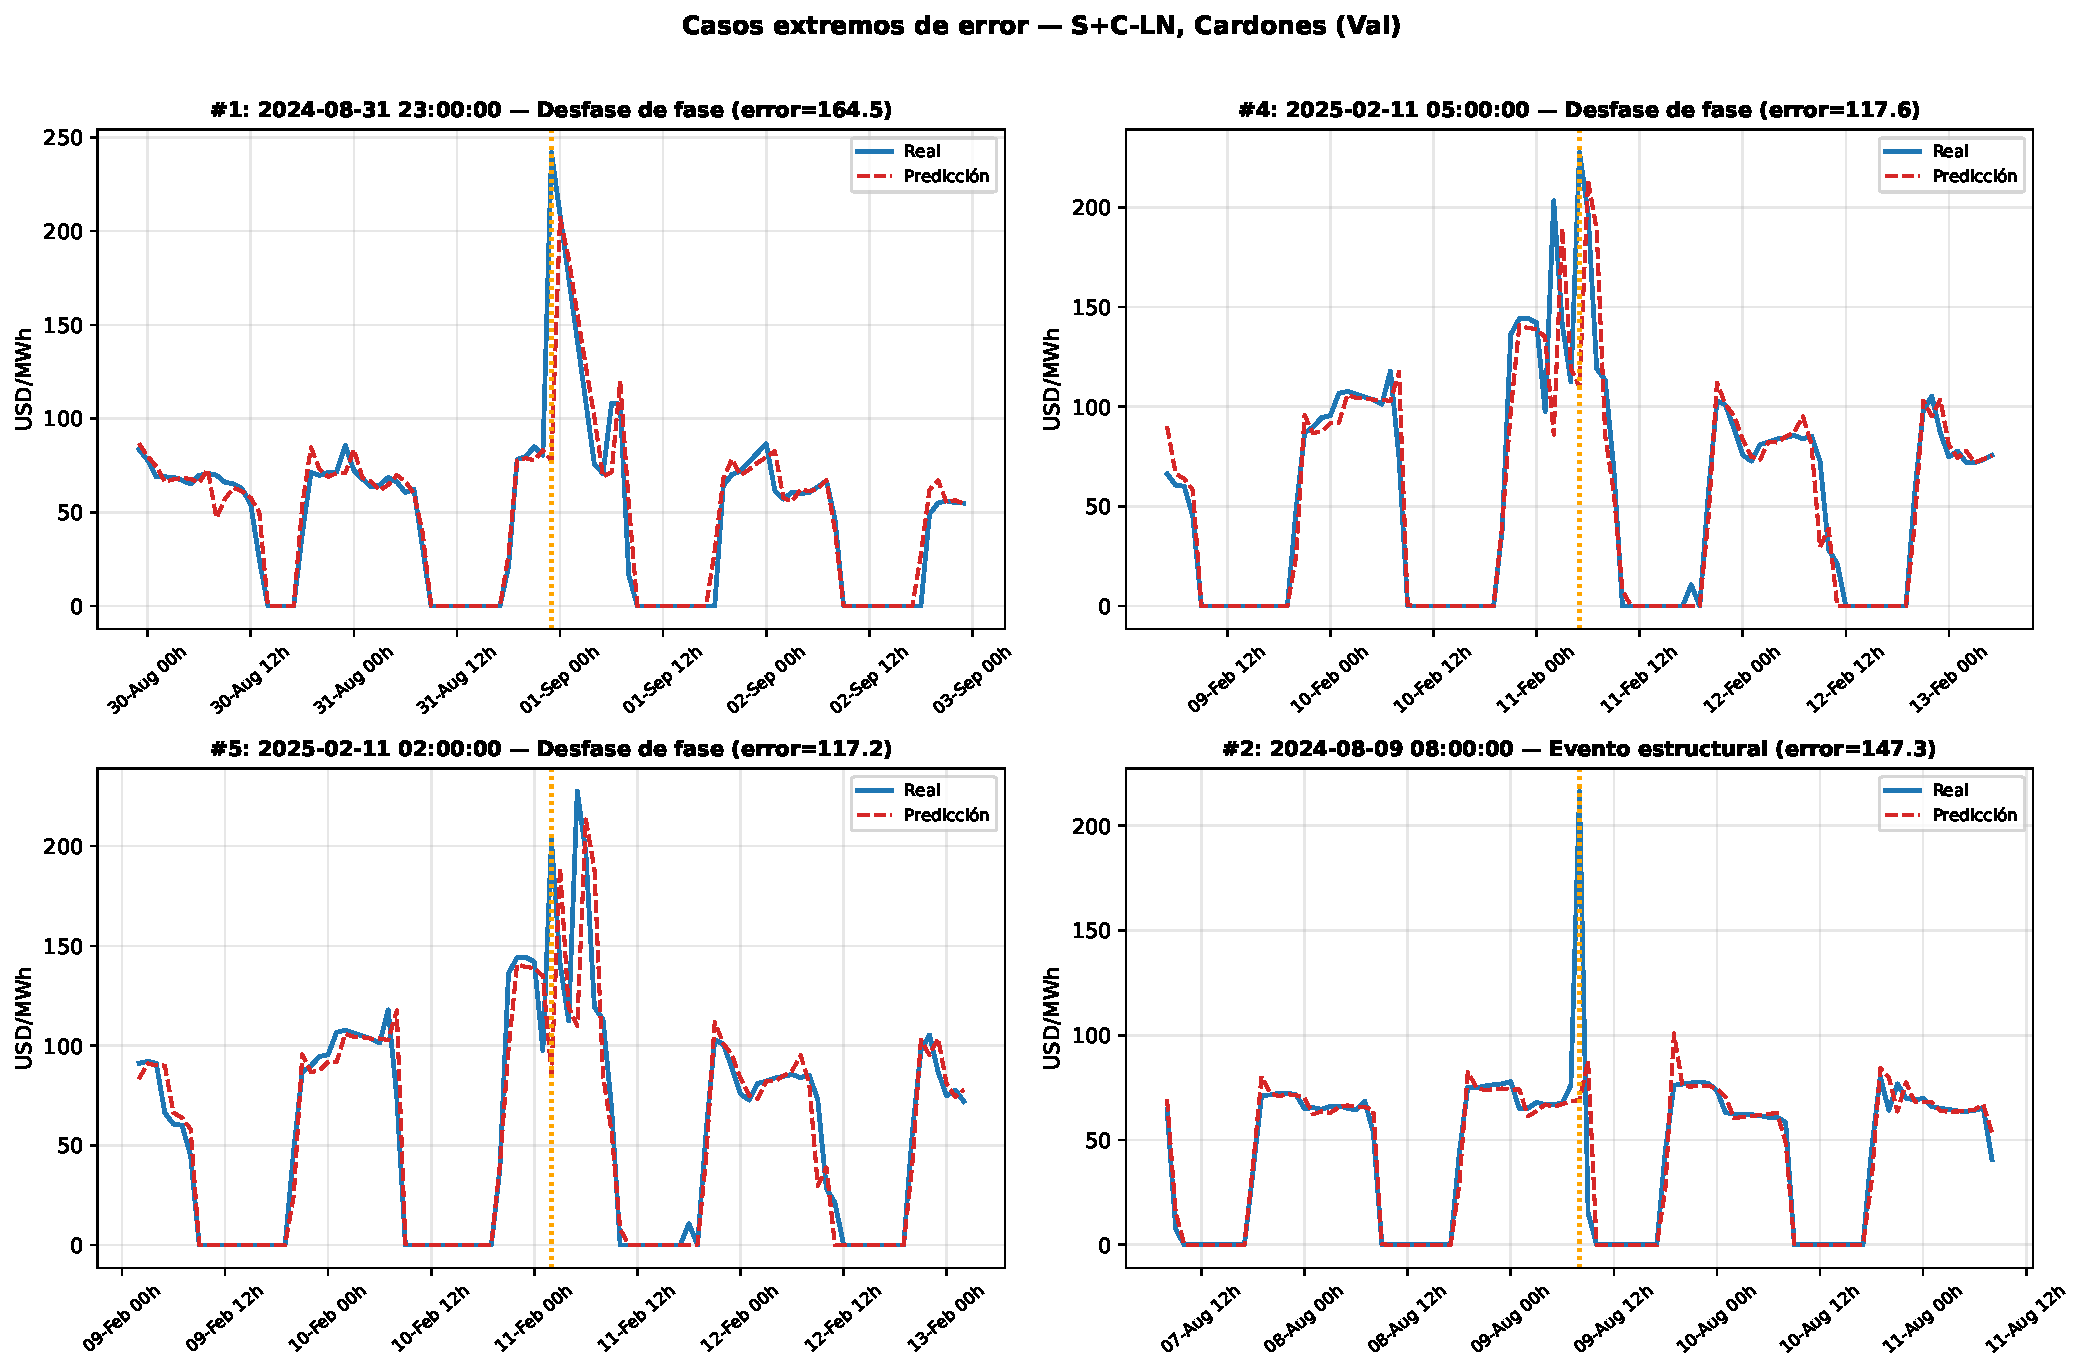
\includegraphics[width=\textwidth]{imagenes/fig_phase_shift_panel_cardones.pdf}
    \caption{Casos extremos de error del $\text{TFT}_\text{LN}$ (S+C), Cardones.}
    \label{fig:phase_shift_panel_cardones}
\end{figure}

\clearpage
\subsection{Charrúa}

\begin{table}[htbp]
    \centering
    \small
    \begin{tabular}{rllrr}
        \toprule
        Rank & Fecha       & Hora  & Error abs.\ (USD/MWh) & Tipo \\
        \midrule
 1 & 2024-08-09 & 08:00 & 132.36 & Desfase de fase \\
 2 & 2024-08-09 & 09:00 & 128.18 & Desfase de fase \\
 3 & 2025-04-01 & 20:00 & 115.24 & Desfase de fase \\
 4 & 2025-02-28 & 10:00 & 114.44 & Desfase de fase \\
 5 & 2025-03-25 & 13:00 & 107.90 & Desfase de fase \\
 6 & 2025-02-26 & 05:00 & 106.61 & Desfase de fase \\
 7 & 2025-03-26 & 09:00 & 105.77 & Evento estructural \\
 8 & 2024-11-25 & 07:00 & 105.55 & Evento estructural \\
 9 & 2025-03-25 & 07:00 & 104.93 & Desfase de fase \\
10 & 2025-04-10 & 07:00 & 100.32 & Desfase de fase \\
11 & 2025-02-11 & 02:00 &  98.89 & Desfase de fase \\
12 & 2025-02-11 & 05:00 &  95.81 & Desfase de fase \\
13 & 2025-04-21 & 01:00 &  95.41 & Desfase de fase \\
14 & 2025-04-06 & 07:00 &  95.32 & Evento estructural \\
15 & 2025-03-27 & 10:00 &  93.44 & Desfase de fase \\
16 & 2025-04-08 & 16:00 &  92.60 & Desfase de fase \\
17 & 2024-06-22 & 18:00 &  92.51 & Desfase de fase \\
18 & 2024-10-03 & 21:00 &  92.20 & Desfase de fase \\
19 & 2025-03-24 & 20:00 &  92.10 & Desfase de fase \\
20 & 2025-04-11 & 08:00 &  91.56 & Desfase de fase \\
        \bottomrule
    \end{tabular}
    \vspace{0.2cm}
    \caption{Los 20 mayores errores absolutos del $\text{TFT}_\text{LN}$ (S+C) en validación, Charrúa.}
    \label{tab:top20_charrua}
\end{table}

\begin{figure}[htbp]
    \centering
    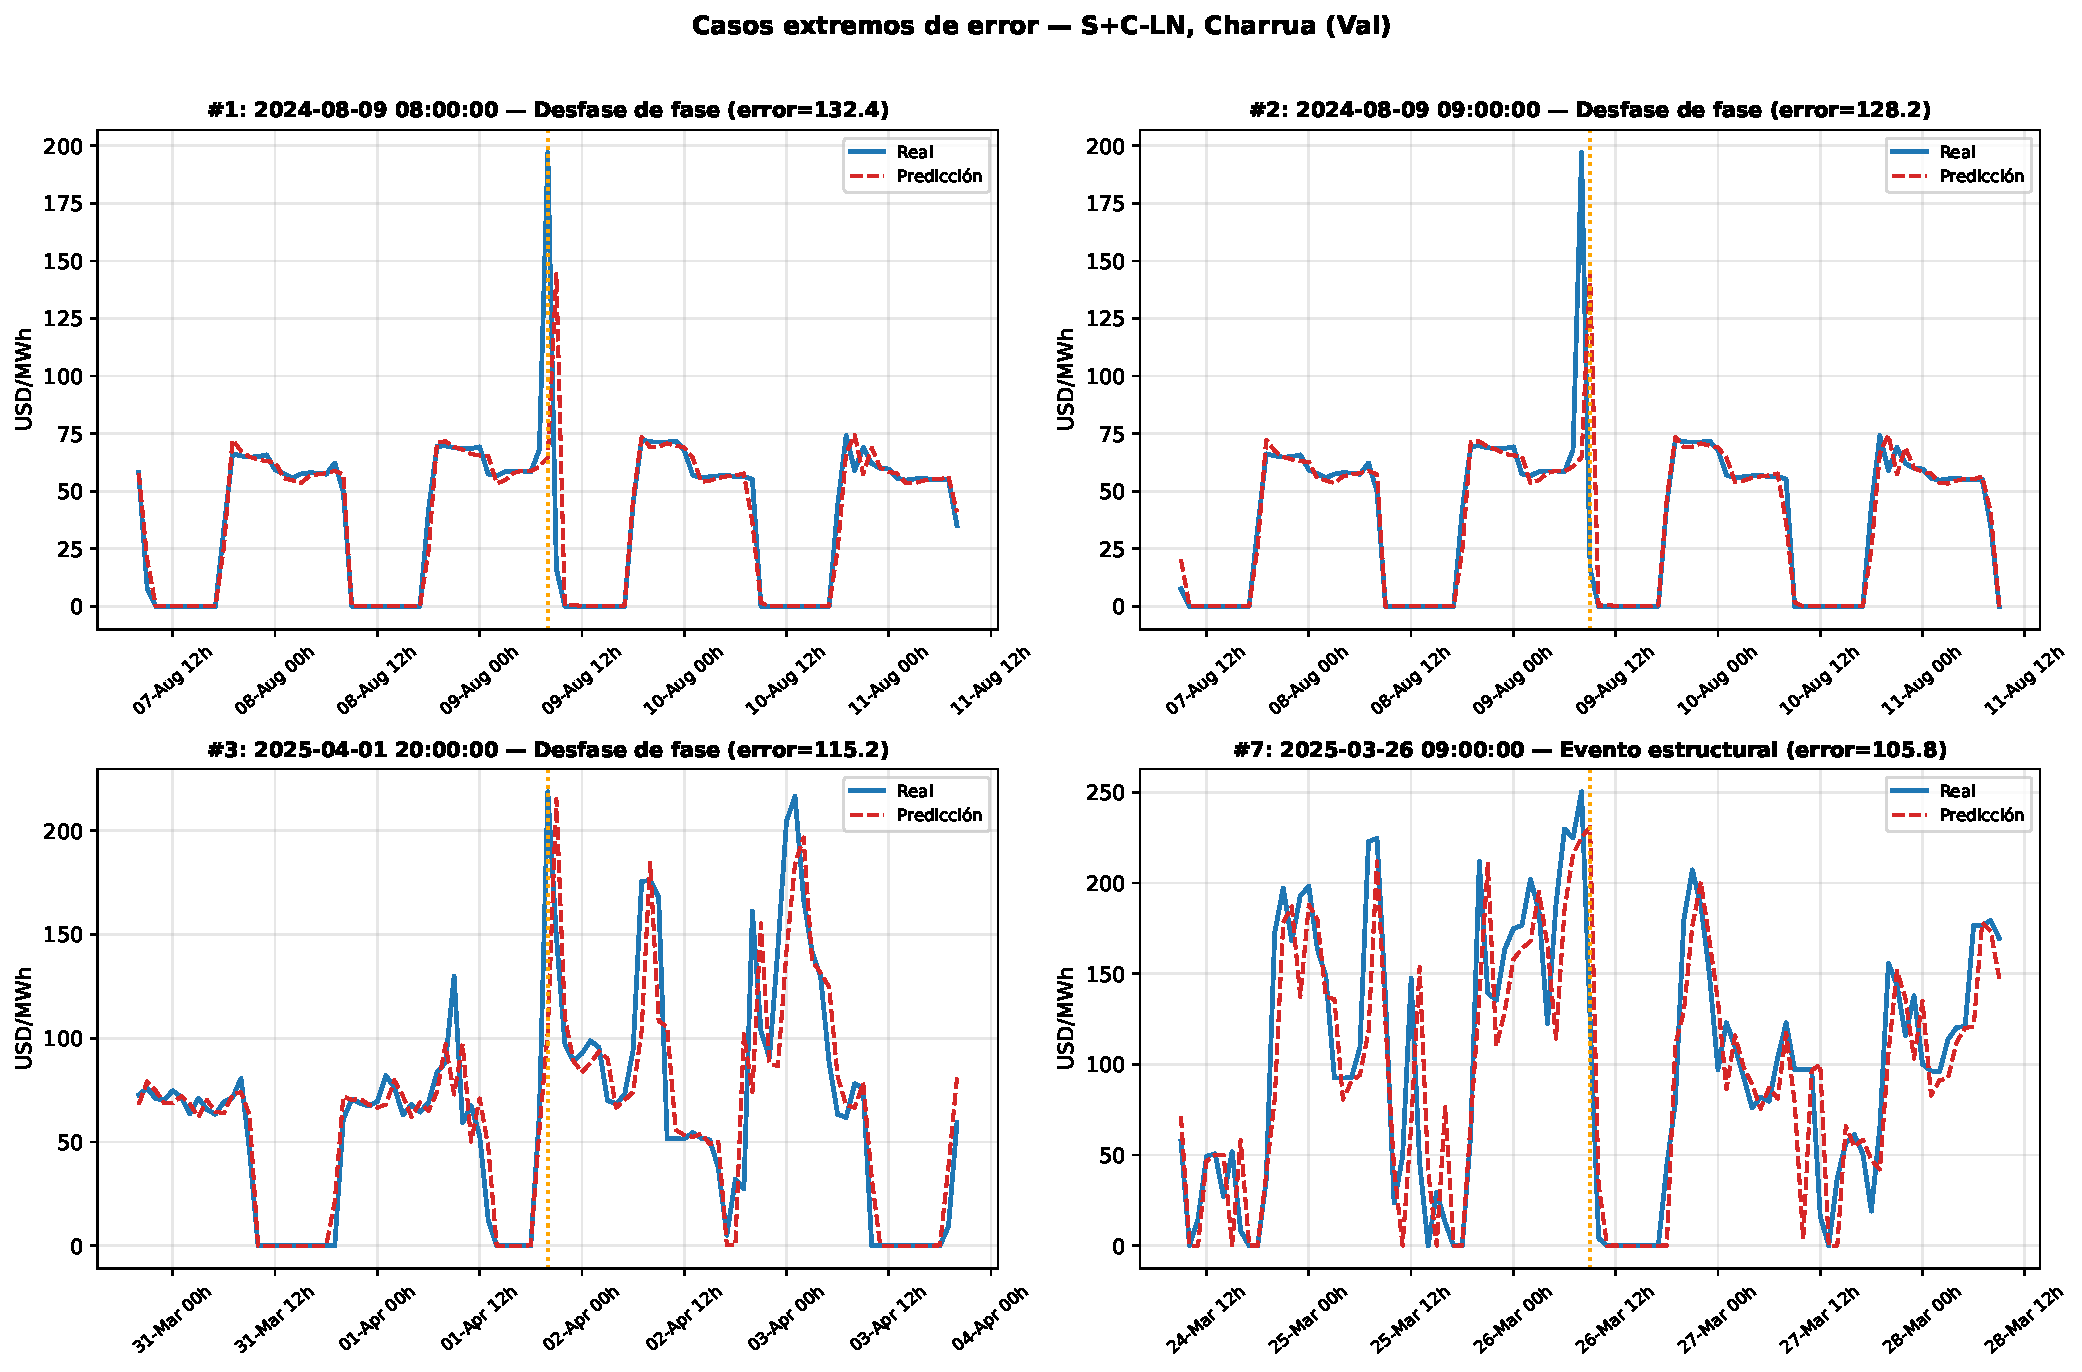
\includegraphics[width=\textwidth]{imagenes/fig_phase_shift_panel_charrua.pdf}
    \caption{Casos extremos de error del $\text{TFT}_\text{LN}$ (S+C), Charrúa.}
    \label{fig:phase_shift_panel_charrua}
\end{figure}

\clearpage
\subsection{Crucero}

\begin{table}[htbp]
    \centering
    \small
    \begin{tabular}{rllrr}
        \toprule
        Rank & Fecha       & Hora  & Error abs.\ (USD/MWh) & Tipo \\
        \midrule
 1 & 2024-08-31 & 23:00 & 174.38 & Desfase de fase \\
 2 & 2024-09-03 & 21:00 & 155.89 & Desfase de fase \\
 3 & 2024-08-09 & 08:00 & 152.69 & Evento estructural \\
 4 & 2024-11-25 & 07:00 & 136.43 & Evento estructural \\
 5 & 2025-02-11 & 02:00 & 128.65 & Desfase de fase \\
 6 & 2025-02-11 & 05:00 & 126.79 & Desfase de fase \\
 7 & 2024-09-04 & 19:00 & 122.14 & Desfase de fase \\
 8 & 2024-09-04 & 03:00 & 115.40 & Desfase de fase \\
 9 & 2025-03-25 & 07:00 & 114.71 & Desfase de fase \\
10 & 2024-10-03 & 21:00 & 113.51 & Desfase de fase \\
11 & 2024-10-04 & 07:00 & 110.96 & Desfase de fase \\
12 & 2025-04-01 & 20:00 & 107.42 & Desfase de fase \\
13 & 2025-04-10 & 07:00 & 104.85 & Desfase de fase \\
14 & 2025-04-21 & 20:00 & 104.33 & Desfase de fase \\
15 & 2024-11-08 & 23:00 & 103.60 & Desfase de fase \\
16 & 2025-04-19 & 21:00 & 101.84 & Desfase de fase \\
17 & 2025-05-05 & 19:00 &  99.22 & Desfase de fase \\
18 & 2024-09-27 & 00:00 &  98.65 & Desfase de fase \\
19 & 2024-10-04 & 00:00 &  98.04 & Desfase de fase \\
20 & 2025-03-25 & 20:00 &  97.99 & Desfase de fase \\
        \bottomrule
    \end{tabular}
    \vspace{0.2cm}
    \caption{Los 20 mayores errores absolutos del $\text{TFT}_\text{LN}$ (S+C) en validación, Crucero.}
    \label{tab:top20_crucero}
\end{table}

\begin{figure}[htbp]
    \centering
    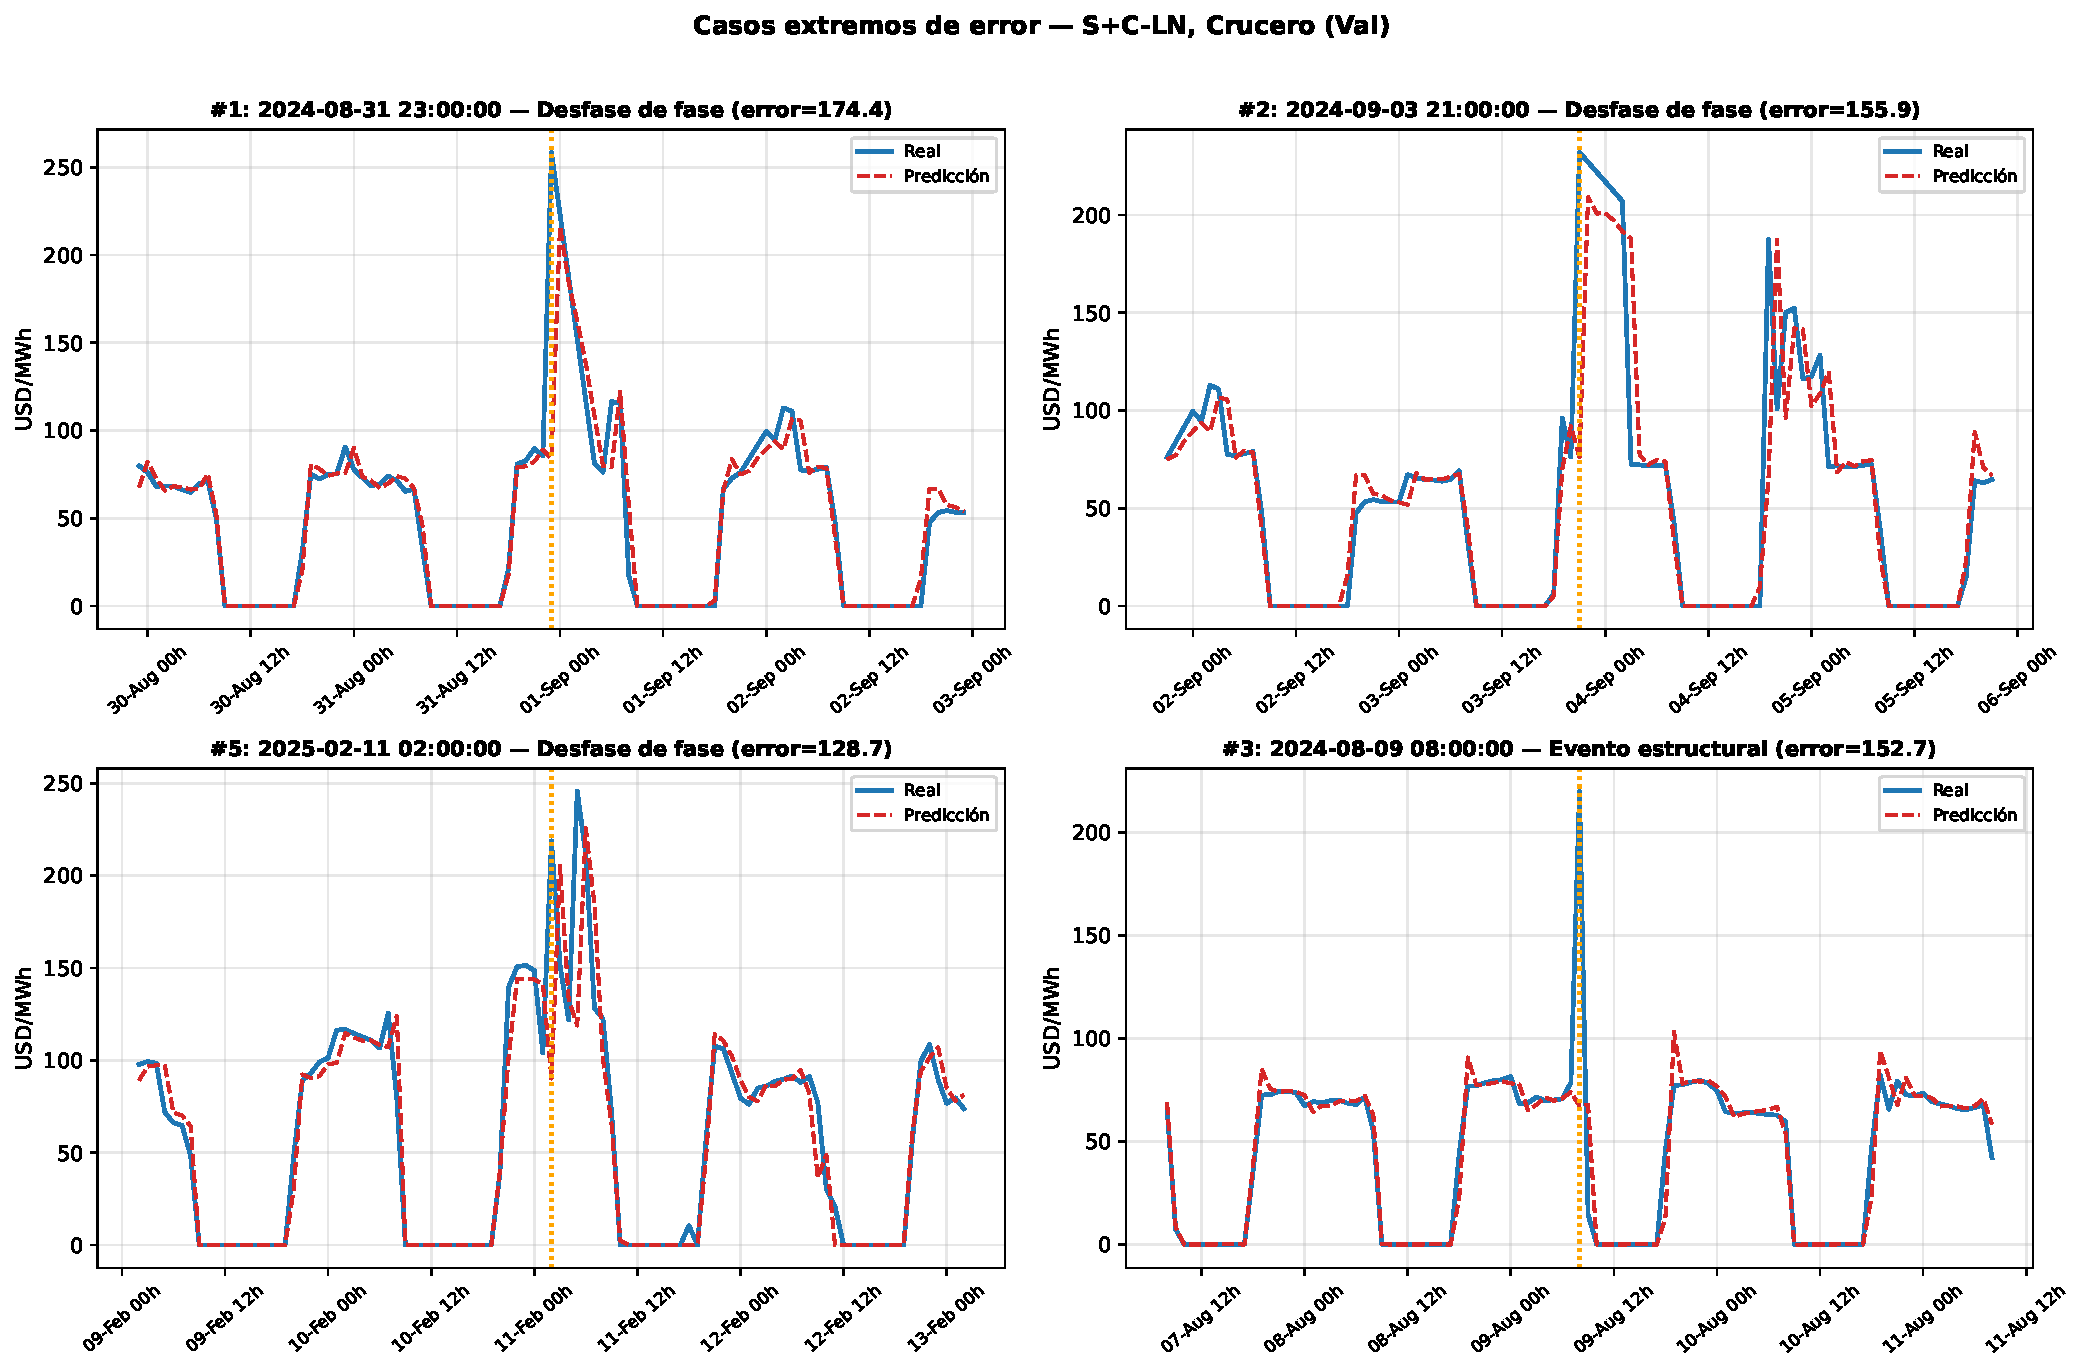
\includegraphics[width=\textwidth]{imagenes/fig_phase_shift_panel_crucero.pdf}
    \caption{Casos extremos de error del $\text{TFT}_\text{LN}$ (S+C), Crucero.}
    \label{fig:phase_shift_panel_crucero}
\end{figure}

\clearpage
\subsection{Pan de Azúcar}

\begin{table}[htbp]
    \centering
    \small
    \begin{tabular}{rllrr}
        \toprule
        Rank & Fecha       & Hora  & Error abs.\ (USD/MWh) & Tipo \\
        \midrule
 1 & 2024-08-09 & 08:00 & 143.70 & Evento estructural \\
 2 & 2025-04-09 & 10:00 & 141.93 & Desfase de fase \\
 3 & 2024-11-25 & 07:00 & 121.17 & Evento estructural \\
 4 & 2025-02-11 & 05:00 & 116.00 & Desfase de fase \\
 5 & 2025-02-28 & 10:00 & 114.26 & Desfase de fase \\
 6 & 2025-03-25 & 07:00 & 114.06 & Desfase de fase \\
 7 & 2025-04-10 & 07:00 & 113.39 & Desfase de fase \\
 8 & 2025-02-11 & 02:00 & 112.29 & Desfase de fase \\
 9 & 2024-10-03 & 21:00 & 108.08 & Desfase de fase \\
10 & 2025-04-01 & 20:00 & 102.58 & Desfase de fase \\
11 & 2025-04-19 & 21:00 & 101.46 & Desfase de fase \\
12 & 2024-10-09 & 09:00 &  99.98 & Desfase de fase \\
13 & 2025-03-25 & 20:00 &  98.47 & Desfase de fase \\
14 & 2025-04-08 & 16:00 &  97.98 & Desfase de fase \\
15 & 2025-02-26 & 05:00 &  97.62 & Desfase de fase \\
16 & 2025-04-06 & 07:00 &  95.02 & Evento estructural \\
17 & 2024-11-08 & 23:00 &  94.82 & Desfase de fase \\
18 & 2024-09-27 & 00:00 &  93.71 & Desfase de fase \\
19 & 2024-10-04 & 07:00 &  91.10 & Desfase de fase \\
20 & 2025-04-21 & 01:00 &  90.23 & Desfase de fase \\
        \bottomrule
    \end{tabular}
    \vspace{0.2cm}
    \caption{Los 20 mayores errores absolutos del $\text{TFT}_\text{LN}$ (S+C) en validación, Pan de Azúcar.}
    \label{tab:top20_pazucar}
\end{table}

\begin{figure}[htbp]
    \centering
    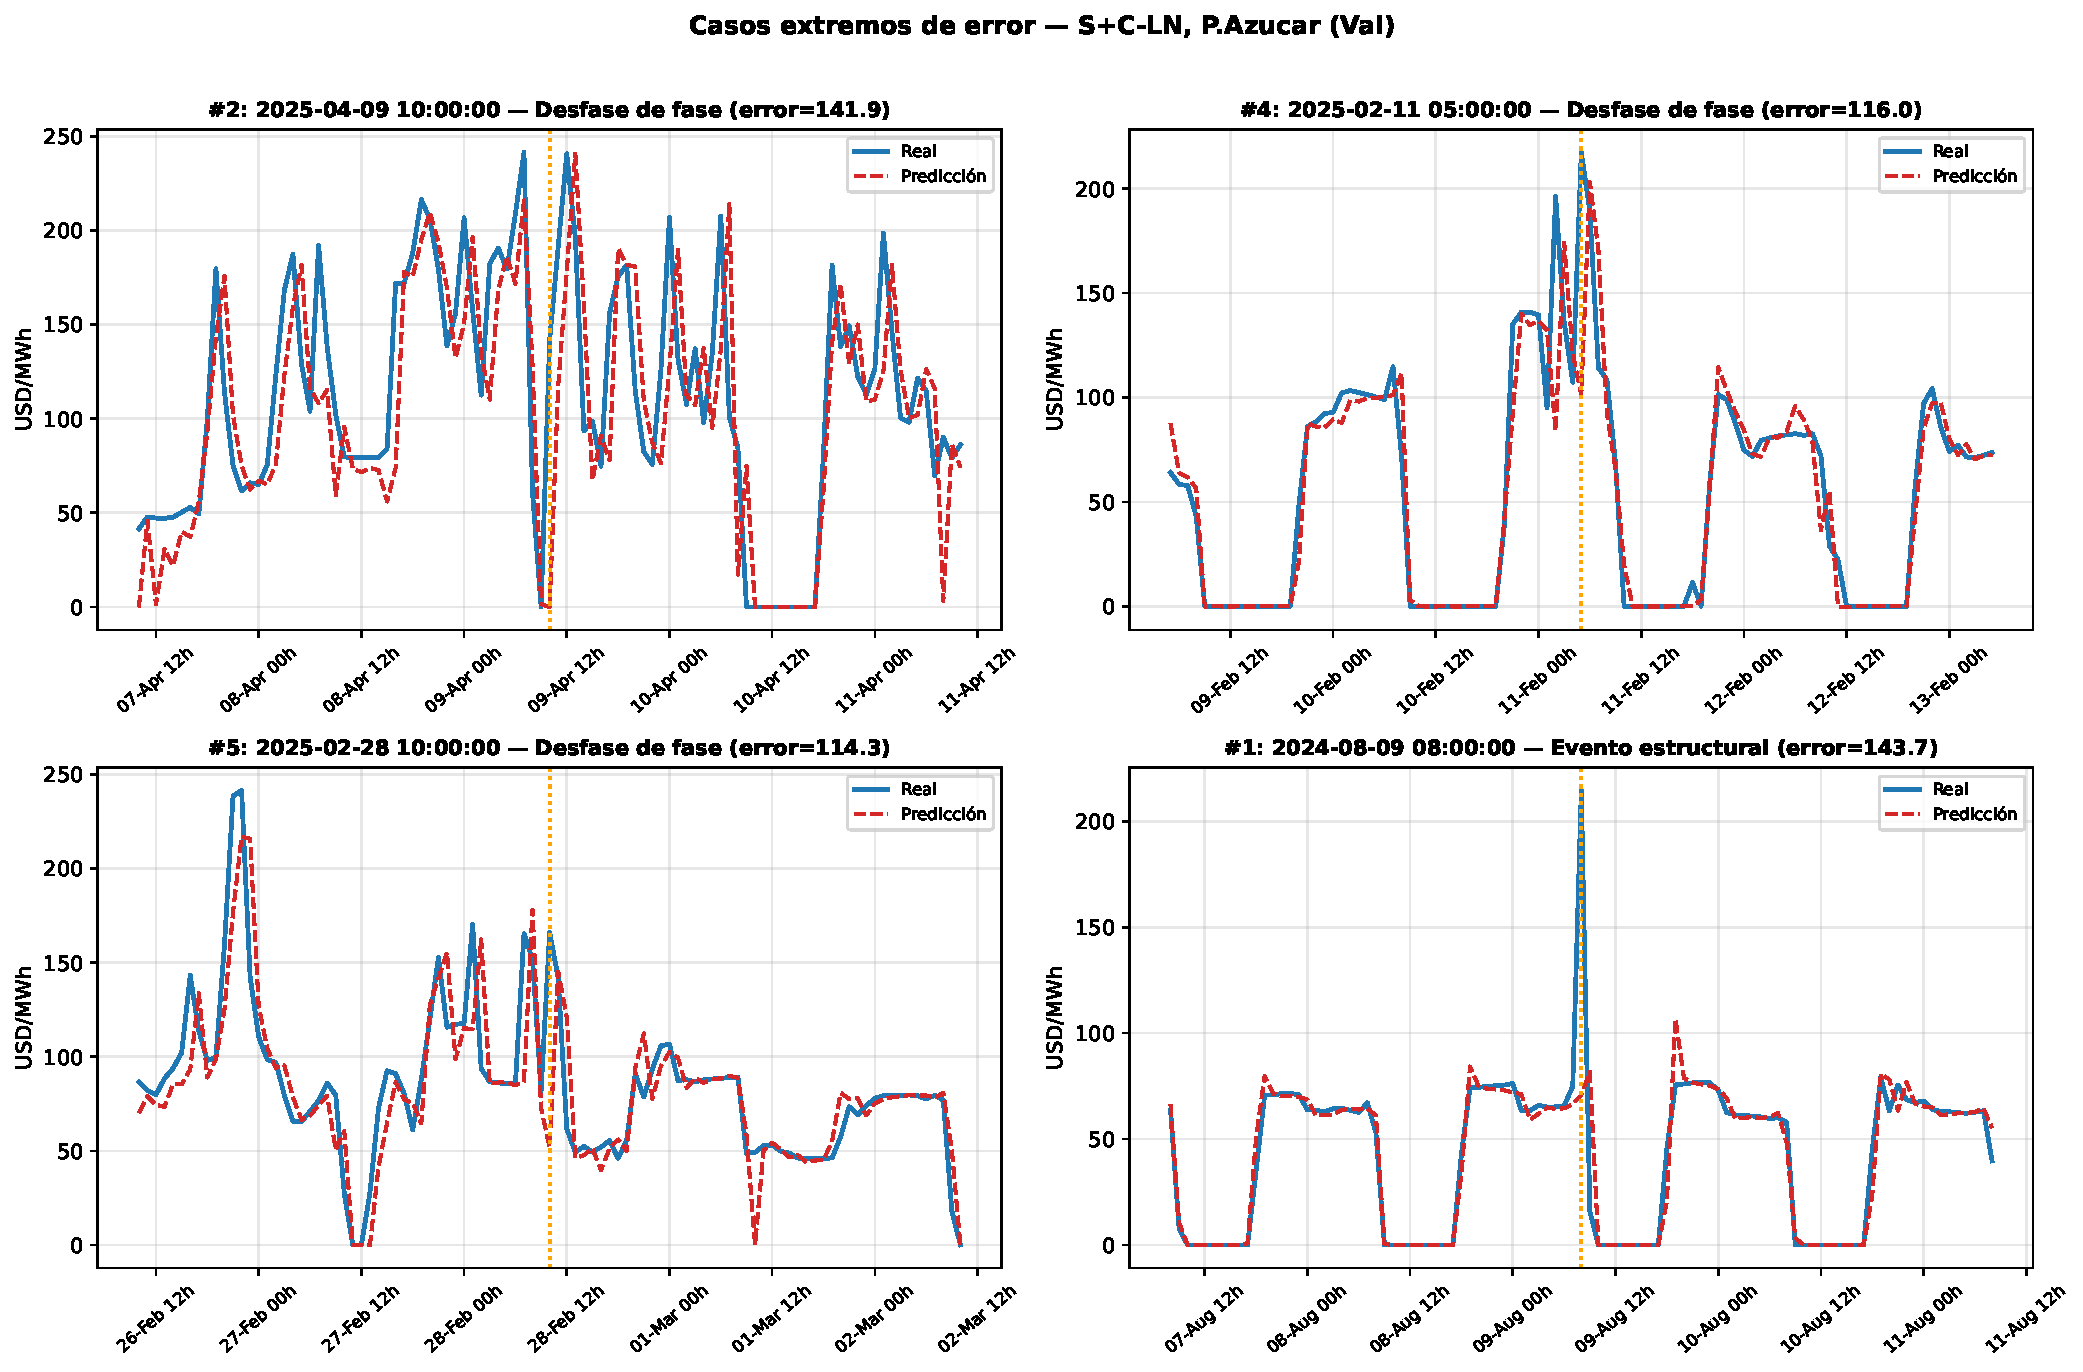
\includegraphics[width=\textwidth]{imagenes/fig_phase_shift_panel_pazucar.pdf}
    \caption{Casos extremos de error del $\text{TFT}_\text{LN}$ (S+C), Pan de Azúcar.}
    \label{fig:phase_shift_panel_pazucar}
\end{figure}

\clearpage
\subsection{Puerto Montt}

\begin{table}[htbp]
    \centering
    \small
    \begin{tabular}{rllrr}
        \toprule
        Rank & Fecha       & Hora  & Error abs.\ (USD/MWh) & Tipo \\
        \midrule
 1 & 2024-08-08 & 10:00 & 241.73 & Desfase de fase \\
 2 & 2025-01-31 & 09:00 & 230.86 & Desfase de fase \\
 3 & 2025-02-01 & 10:00 & 221.28 & Desfase de fase \\
 4 & 2025-02-17 & 10:00 & 218.87 & Desfase de fase \\
 5 & 2024-07-27 & 10:00 & 215.08 & Desfase de fase \\
 6 & 2024-07-21 & 01:00 & 211.68 & Desfase de fase \\
 7 & 2024-08-07 & 11:00 & 207.02 & Desfase de fase \\
 8 & 2025-02-09 & 12:00 & 205.38 & Desfase de fase \\
 9 & 2025-02-14 & 20:00 & 198.06 & Desfase de fase \\
10 & 2025-02-08 & 05:00 & 196.61 & Desfase de fase \\
11 & 2025-01-09 & 11:00 & 195.40 & Desfase de fase \\
12 & 2024-07-22 & 12:00 & 191.37 & Desfase de fase \\
13 & 2025-02-16 & 12:00 & 190.55 & Desfase de fase \\
14 & 2025-01-30 & 18:00 & 188.20 & Desfase de fase \\
15 & 2024-07-29 & 16:00 & 188.11 & Desfase de fase \\
16 & 2025-01-12 & 16:00 & 183.57 & Desfase de fase \\
17 & 2024-07-21 & 02:00 & 183.27 & Desfase de fase \\
18 & 2025-02-09 & 11:00 & 183.13 & Desfase de fase \\
19 & 2024-07-30 & 13:00 & 182.82 & Desfase de fase \\
20 & 2024-07-29 & 11:00 & 182.36 & Desfase de fase \\
        \bottomrule
    \end{tabular}
    \vspace{0.2cm}
    \caption{Los 20 mayores errores absolutos del $\text{TFT}_\text{LN}$ (S+C) en validación, Puerto Montt. A diferencia del resto de las barras, ninguno cae en horas de transición solar (07:00--08:00, 19:00--21:00) ni comparte fecha con los eventos de las demás barras, consistente con una dinámica gobernada por la disponibilidad hidroeléctrica.}
    \label{tab:top20_pmontt}
\end{table}

\begin{figure}[htbp]
    \centering
    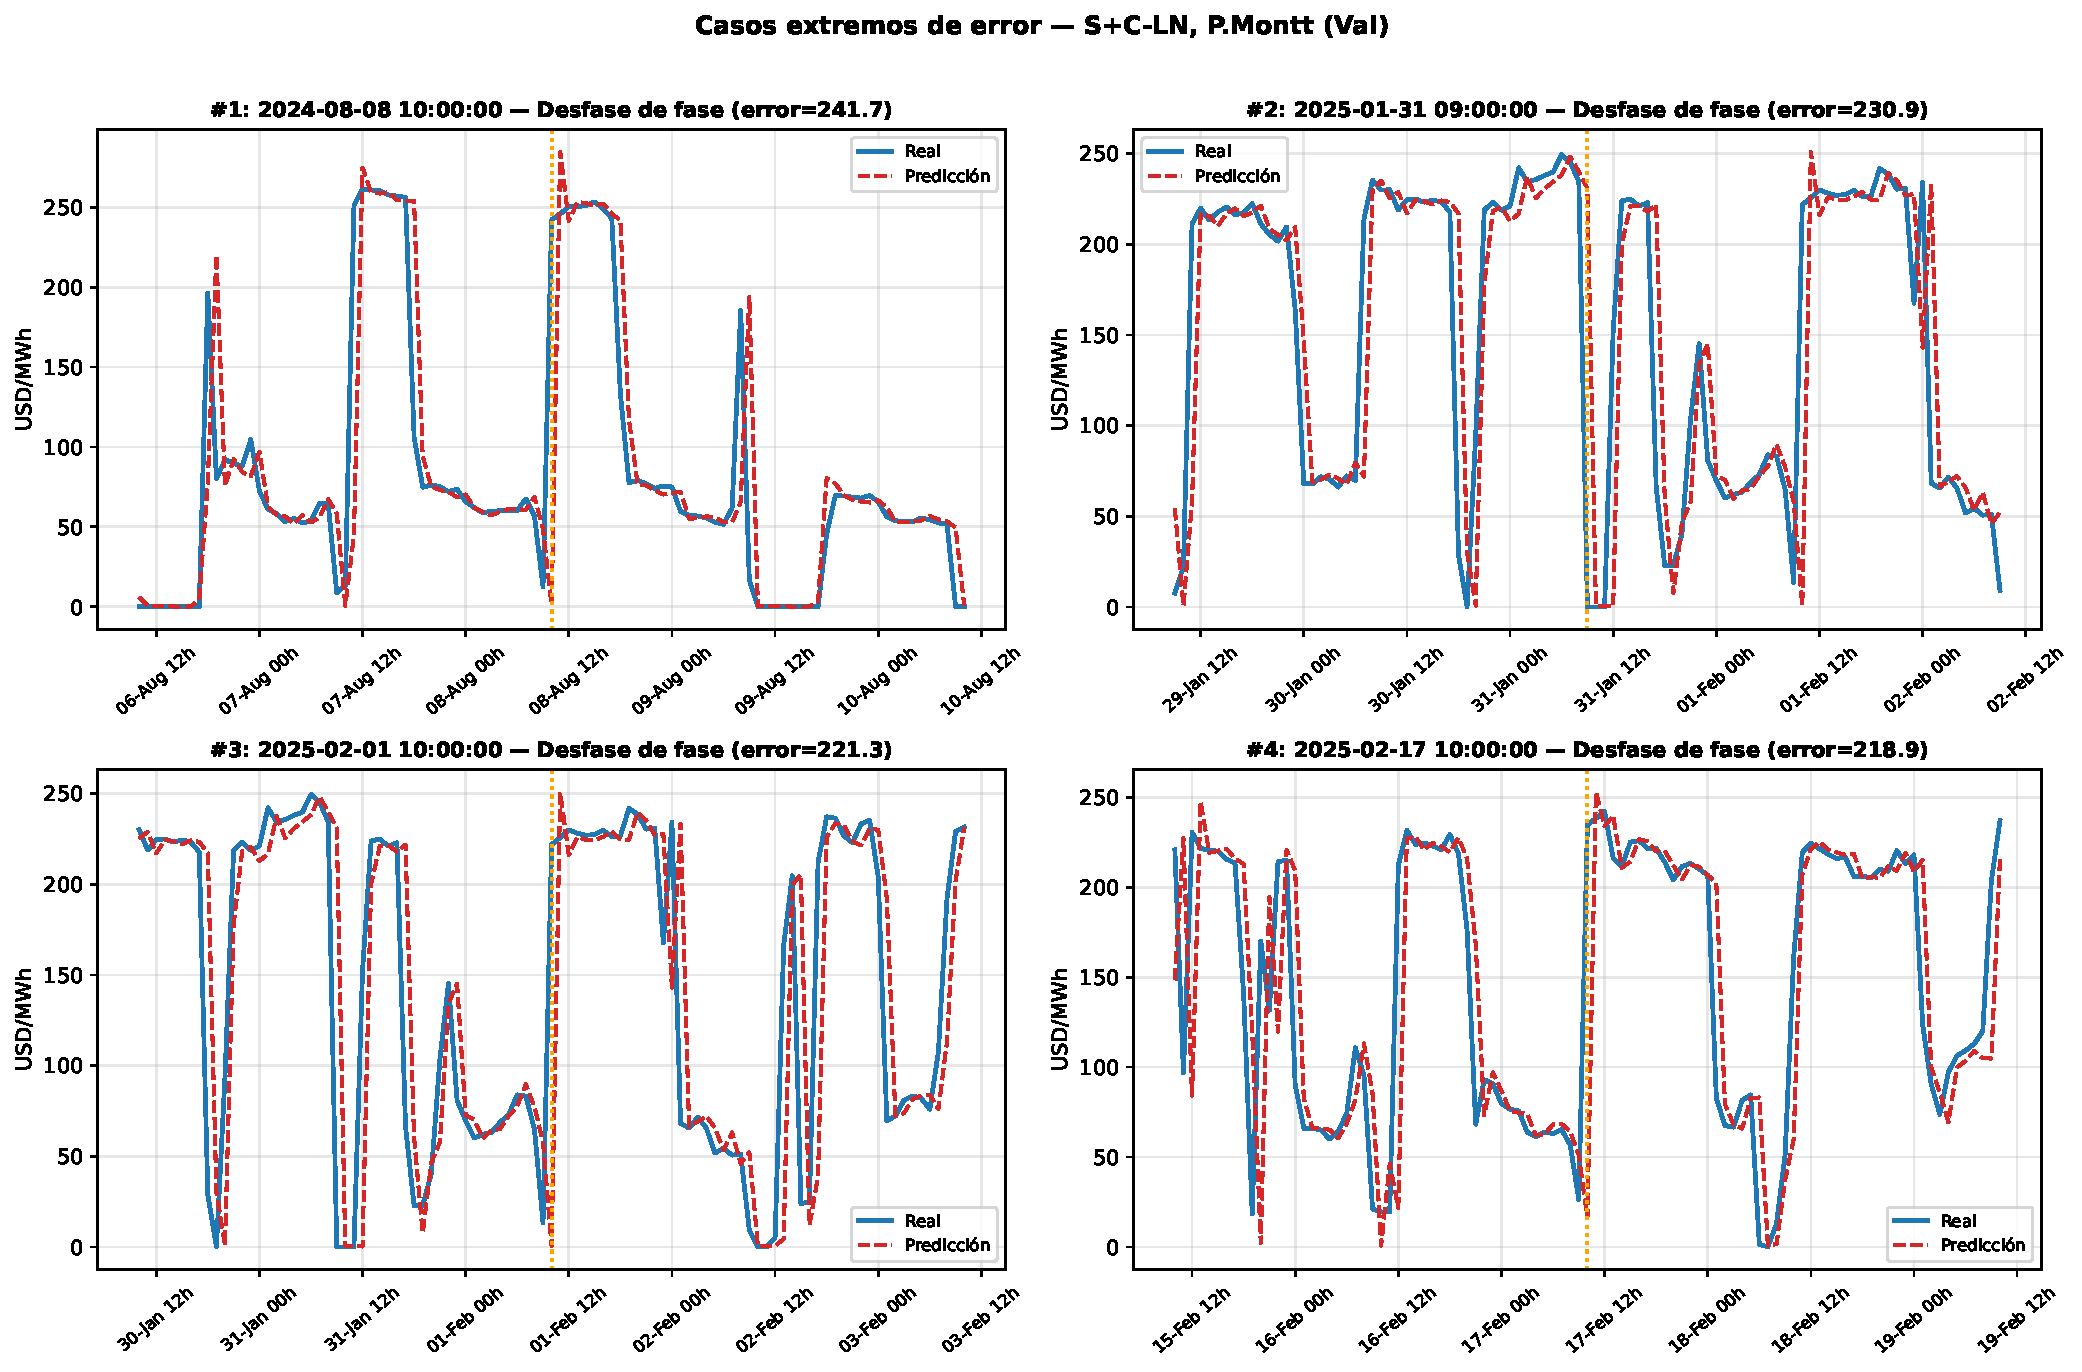
\includegraphics[width=\textwidth]{imagenes/fig_phase_shift_panel_pmontt.pdf}
    \caption{Casos extremos de error del $\text{TFT}_\text{LN}$ (S+C), Puerto Montt.}
    \label{fig:phase_shift_panel_pmontt}
\end{figure}

\clearpage
\subsection{Quillota}

\begin{table}[htbp]
    \centering
    \small
    \begin{tabular}{rllrr}
        \toprule
        Rank & Fecha       & Hora  & Error abs.\ (USD/MWh) & Tipo \\
        \midrule
 1 & 2024-08-09 & 08:00 & 144.20 & Evento estructural \\
 2 & 2025-04-01 & 20:00 & 136.59 & Desfase de fase \\
 3 & 2025-04-10 & 07:00 & 133.54 & Desfase de fase \\
 4 & 2025-04-09 & 09:00 & 122.63 & Desfase de fase \\
 5 & 2025-02-28 & 10:00 & 115.66 & Desfase de fase \\
 6 & 2024-11-25 & 07:00 & 113.03 & Evento estructural \\
 7 & 2025-03-25 & 07:00 & 110.41 & Desfase de fase \\
 8 & 2024-10-03 & 21:00 & 105.31 & Desfase de fase \\
 9 & 2025-02-11 & 05:00 & 105.15 & Desfase de fase \\
10 & 2025-04-06 & 07:00 & 104.96 & Evento estructural \\
11 & 2025-02-26 & 05:00 & 102.50 & Desfase de fase \\
12 & 2025-02-11 & 02:00 & 101.02 & Desfase de fase \\
13 & 2025-04-21 & 01:00 &  95.57 & Desfase de fase \\
14 & 2024-06-22 & 18:00 &  95.36 & Desfase de fase \\
15 & 2024-06-17 & 23:00 &  92.82 & Evento estructural \\
16 & 2025-04-11 & 08:00 &  92.05 & Desfase de fase \\
17 & 2024-11-08 & 23:00 &  91.39 & Desfase de fase \\
18 & 2025-03-25 & 13:00 &  91.01 & Desfase de fase \\
19 & 2025-03-27 & 10:00 &  90.81 & Desfase de fase \\
20 & 2025-04-08 & 16:00 &  90.71 & Desfase de fase \\
        \bottomrule
    \end{tabular}
    \vspace{0.2cm}
    \caption{Los 20 mayores errores absolutos del $\text{TFT}_\text{LN}$ (S+C) en validación, Quillota.}
    \label{tab:top20_quillota}
\end{table}

\begin{figure}[htbp]
    \centering
    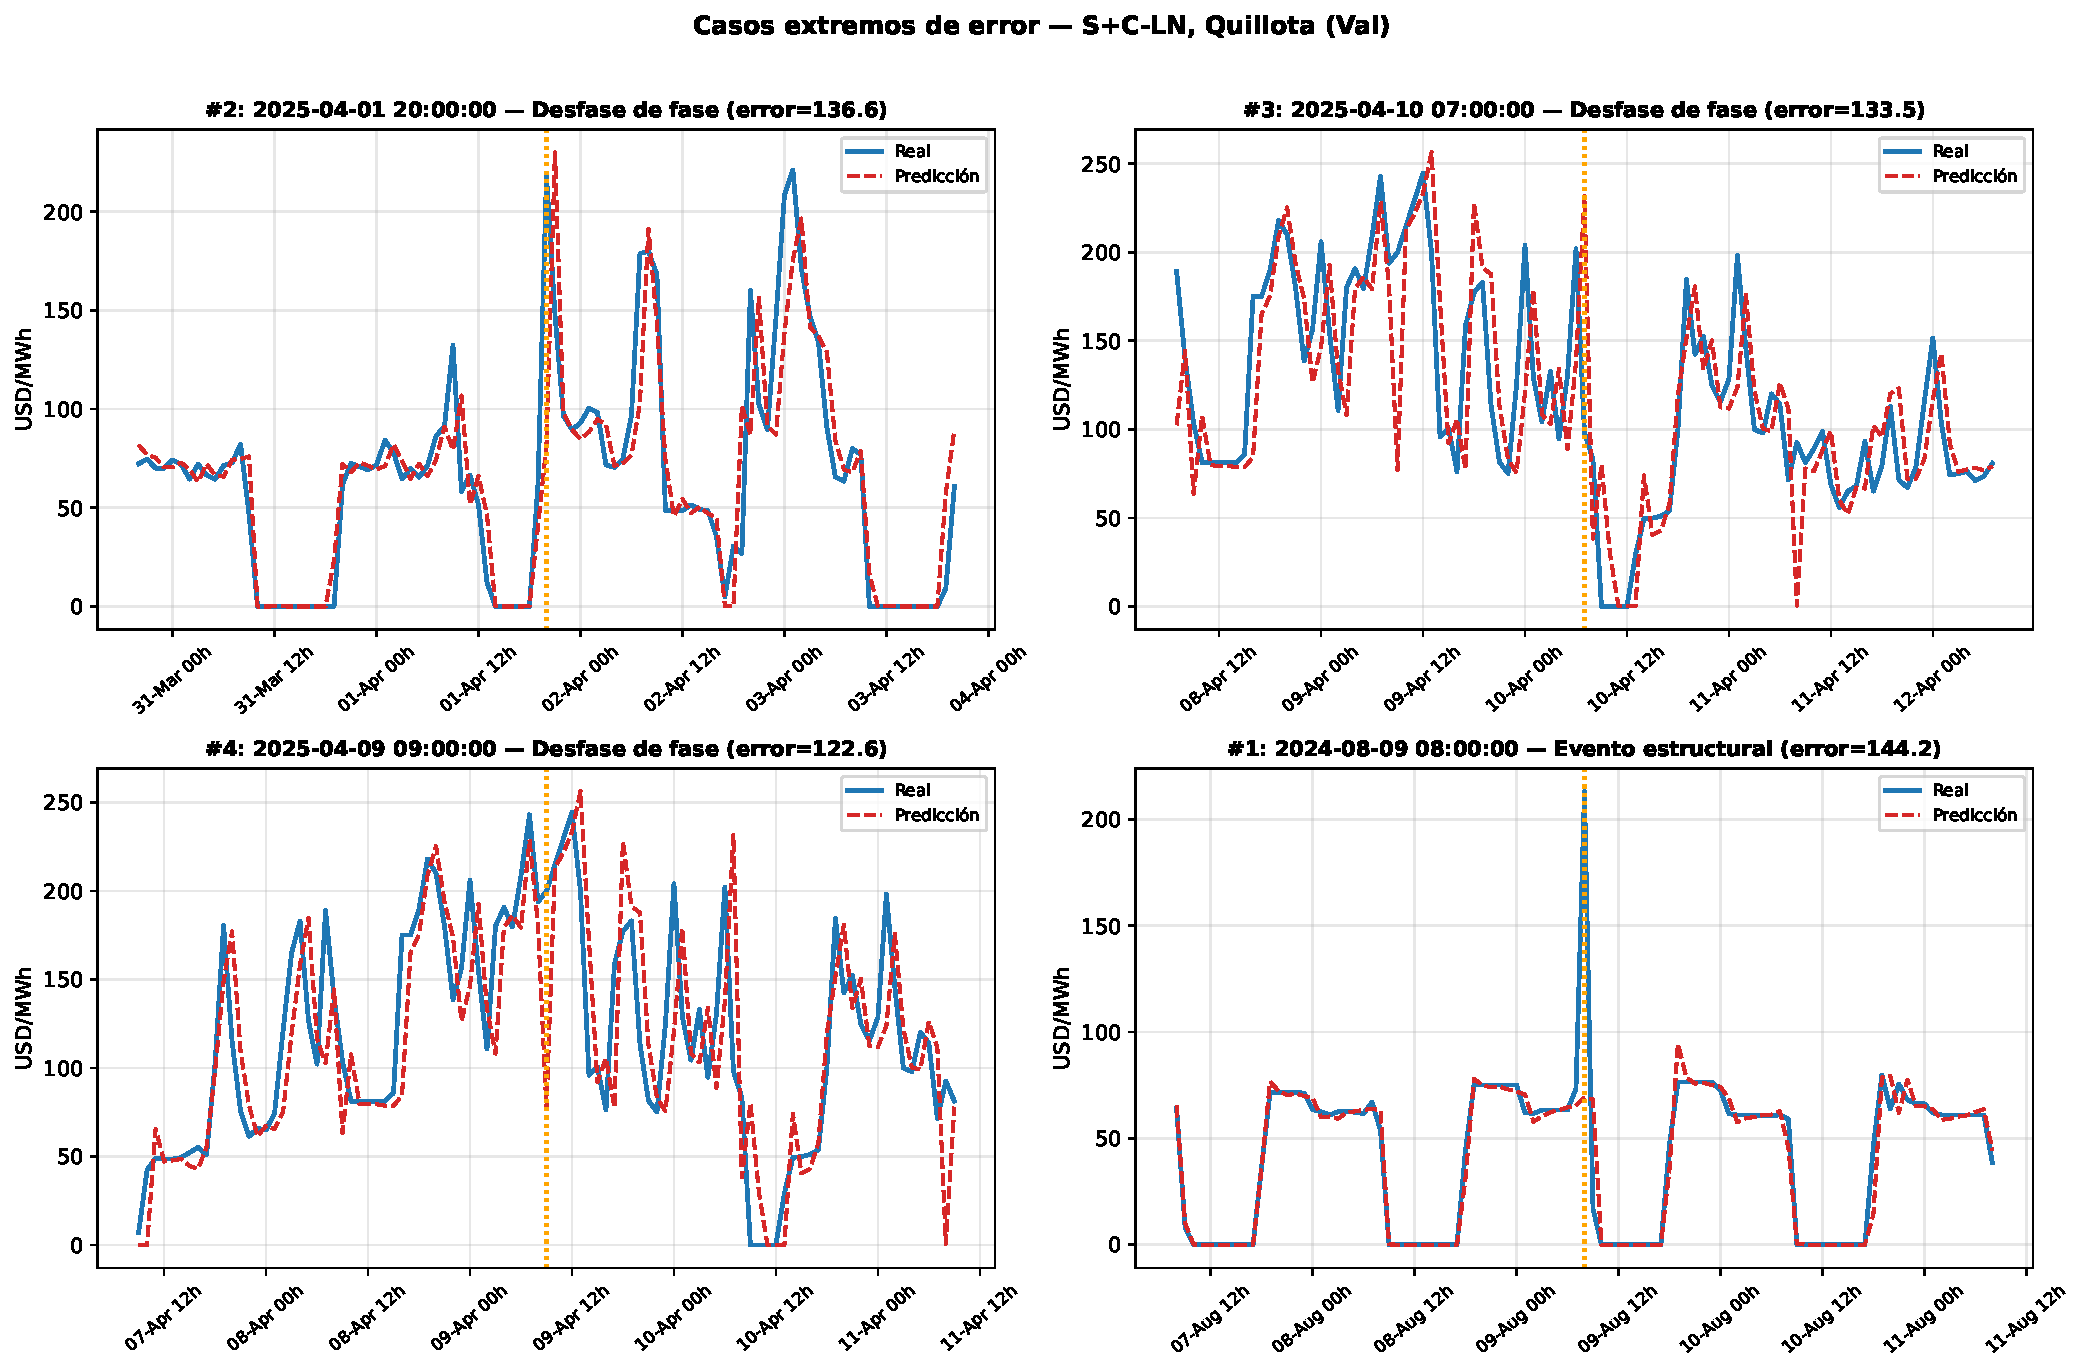
\includegraphics[width=\textwidth]{imagenes/fig_phase_shift_panel_quillota.pdf}
    \caption{Casos extremos de error del $\text{TFT}_\text{LN}$ (S+C), Quillota.}
    \label{fig:phase_shift_panel_quillota}
\end{figure}

\clearpage
\subsection{Tarapacá}

\begin{table}[htbp]
    \centering
    \small
    \begin{tabular}{rllrr}
        \toprule
        Rank & Fecha       & Hora  & Error abs.\ (USD/MWh) & Tipo \\
        \midrule
 1 & 2024-09-03 & 21:00 & 169.64 & Desfase de fase \\
 2 & 2024-08-12 & 20:00 & 167.53 & Desfase de fase \\
 3 & 2024-08-09 & 08:00 & 167.29 & Evento estructural \\
 4 & 2024-11-25 & 07:00 & 143.76 & Evento estructural \\
 5 & 2025-02-11 & 02:00 & 139.15 & Desfase de fase \\
 6 & 2025-02-11 & 05:00 & 135.81 & Desfase de fase \\
 7 & 2025-04-09 & 08:00 & 133.84 & Evento estructural \\
 8 & 2025-04-01 & 20:00 & 130.39 & Desfase de fase \\
 9 & 2025-05-05 & 19:00 & 130.25 & Desfase de fase \\
10 & 2024-09-04 & 19:00 & 128.62 & Desfase de fase \\
11 & 2024-09-04 & 03:00 & 125.70 & Desfase de fase \\
12 & 2024-10-03 & 21:00 & 122.09 & Desfase de fase \\
13 & 2024-10-04 & 07:00 & 120.97 & Desfase de fase \\
14 & 2025-03-25 & 07:00 & 118.13 & Desfase de fase \\
15 & 2024-09-04 & 20:00 & 116.90 & Desfase de fase \\
16 & 2025-03-25 & 20:00 & 116.83 & Desfase de fase \\
17 & 2024-11-08 & 23:00 & 112.64 & Desfase de fase \\
18 & 2024-09-27 & 00:00 & 106.83 & Desfase de fase \\
19 & 2025-04-10 & 07:00 & 106.41 & Desfase de fase \\
20 & 2025-04-19 & 21:00 & 106.34 & Desfase de fase \\
        \bottomrule
    \end{tabular}
    \vspace{0.2cm}
    \caption{Los 20 mayores errores absolutos del $\text{TFT}_\text{LN}$ (S+C) en validación, Tarapacá.}
    \label{tab:top20_tarapaca}
\end{table}

\begin{figure}[htbp]
    \centering
    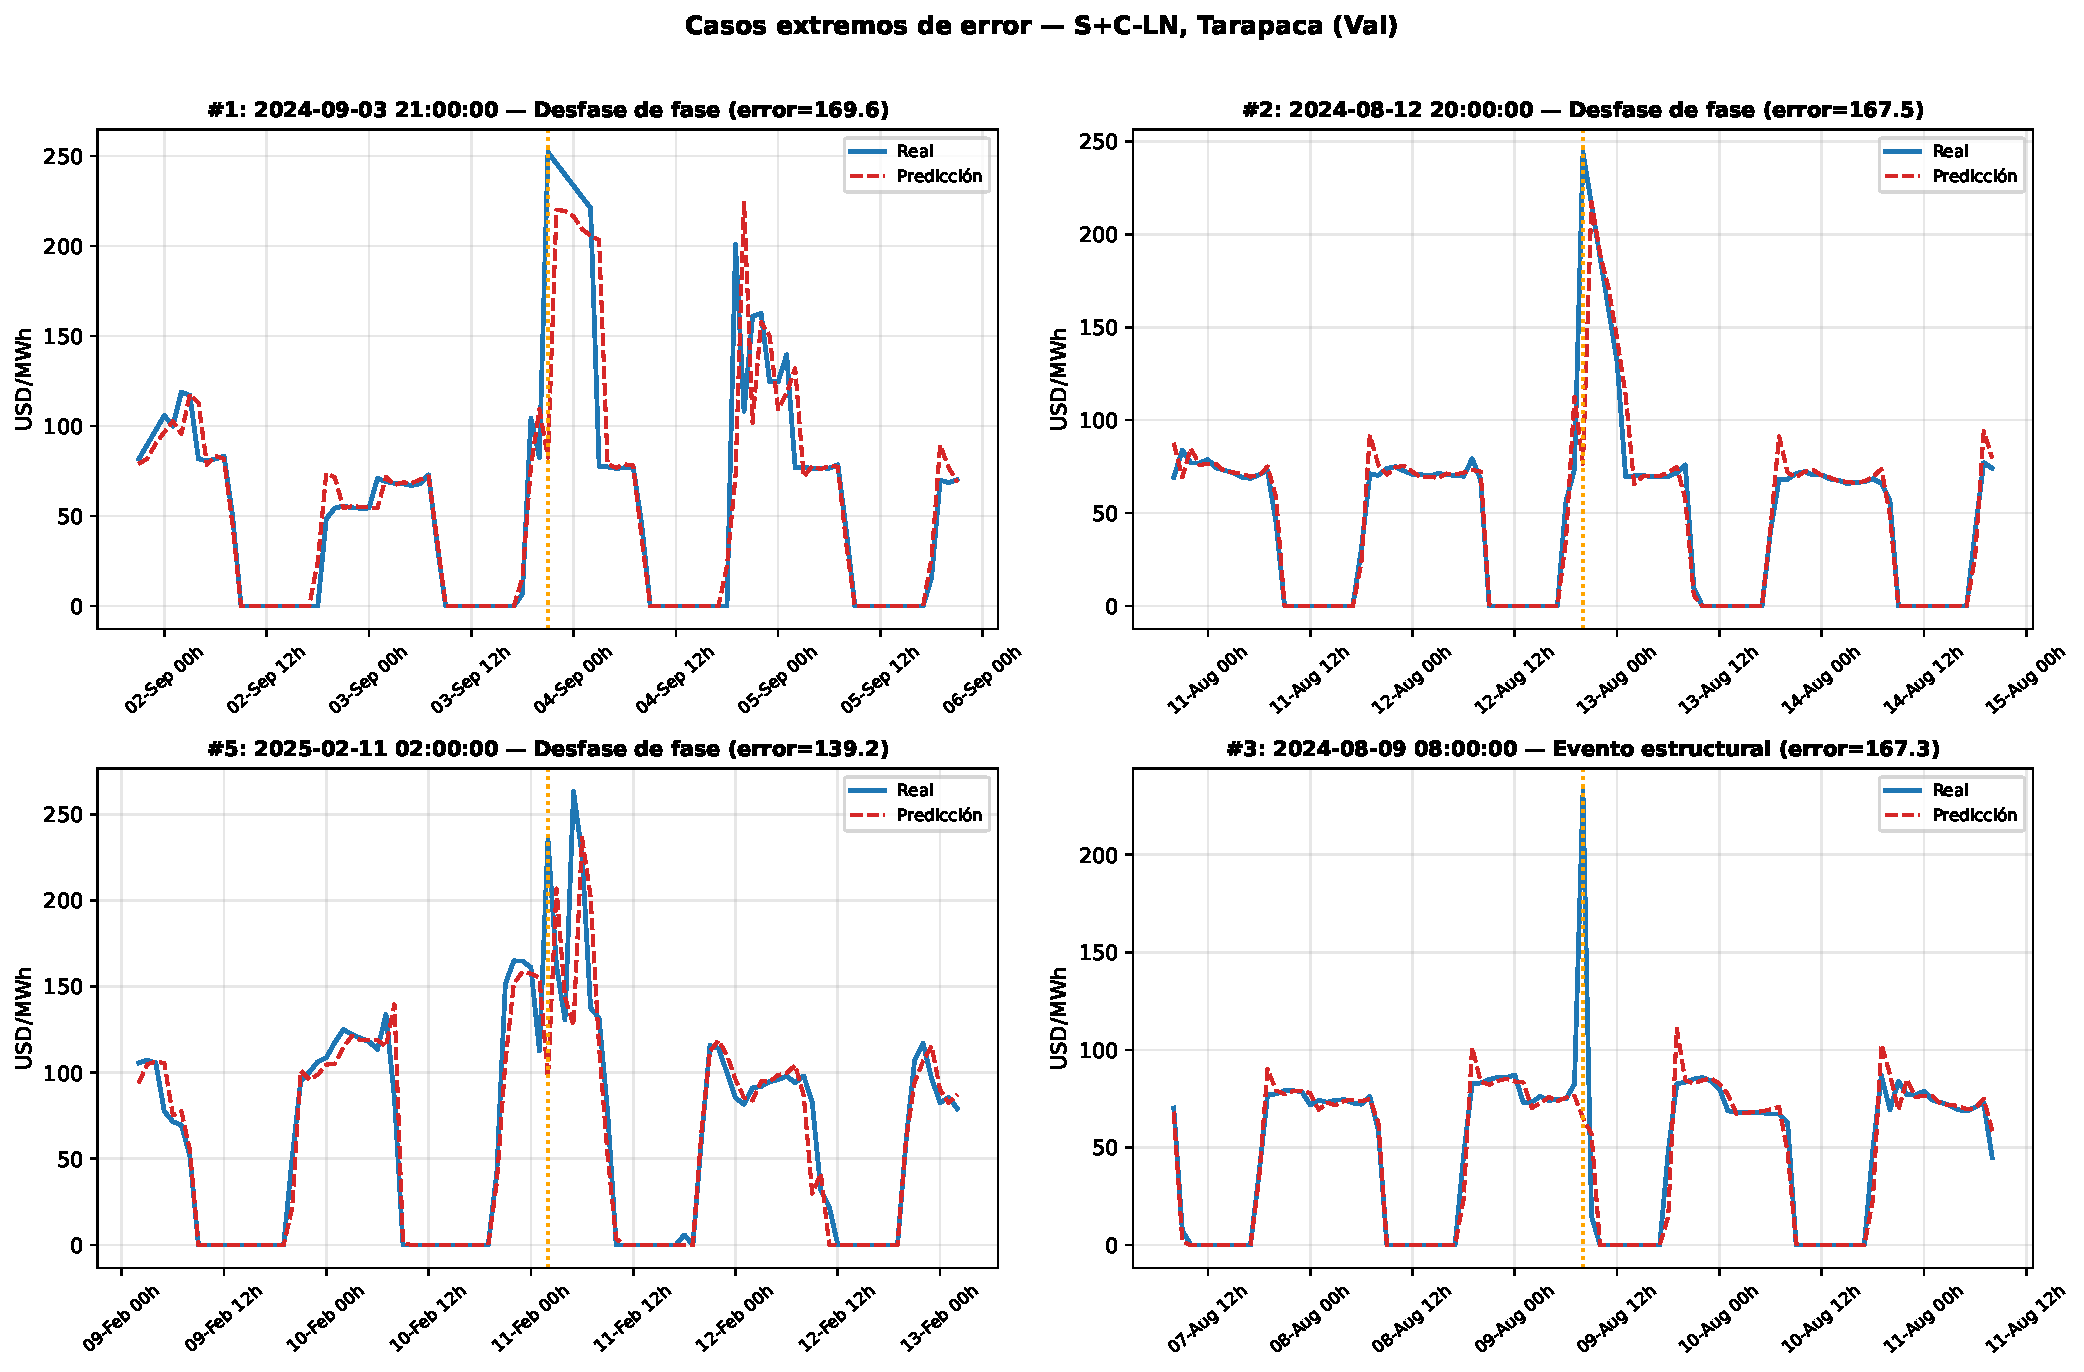
\includegraphics[width=\textwidth]{imagenes/fig_phase_shift_panel_tarapaca.pdf}
    \caption{Casos extremos de error del $\text{TFT}_\text{LN}$ (S+C), Tarapacá.}
    \label{fig:phase_shift_panel_tarapaca}
\end{figure}

\end{appendices}
\end{document}